%%%%%%%%%%%%%%%%%%%%%%%%%%%%%%%%%%%%%%%%%%%%%%%%%%%%%%%%%%%%%%%%
%                                                              %
%   Introducción informal a Matlab y Octave                    %
%   Archivo de fuente de texto LaTeX                           %
%   Guillem Borrell Nogueras et al.                            %
%   Licencia :                                                 %
%     GNU FDL                                                  %
%                                                              %
%   2005-2006-2007-2008                                        %
%                                                              %
%   Builds with both LaTeX and pdfLaTeX                        %
%   Remember to run makeindex                                  %
%%%%%%%%%%%%%%%%%%%%%%%%%%%%%%%%%%%%%%%%%%%%%%%%%%%%%%%%%%%%%%%%

\documentclass[10pt,fleqn,a4]{book}
%   Makeindex support
\usepackage{makeidx}
\makeindex
%   Usual document characteristics
\usepackage[spanish]{babel}
\usepackage[T1]{fontenc}
\usepackage[utf8]{inputenc}
\usepackage{cursomo}
\setlength{\textwidth}{175mm}
\setlength{\oddsidemargin}{-1cm}
\setlength{\evensidemargin}{-1cm}
%%%%%%%%%%%%%%%%%%%%%%%%%%%%%%%%%%%%%%%%%%%%
%                                          %
%                                          %
%      %%%Introducción informal a%%%       %
%      %%%Matlab y Octave        %%%       % 
%                                          %
%                                          %
%%%%%%%%%%%%%%%%%%%%%%%%%%%%%%%%%%%%%%%%%%%%

\begin{document}
\lstset{language=Octave}
\title{\begin{Huge}Introducción informal a Matlab y Octave\end{Huge}}


\author{Guillem Borrell i Nogueras\\
  \texttt{\url{http://iimyo.forja.rediris.es/}}\\
}

\maketitle


Este documento está publicado según la siguiente licencia:
\begin{center}
\begin{Huge}
GNU Free Documentation License
\end{Huge}

\end{center}

\bigskip
\begin{quote}
    Copyright \copyright{}  2005-2008  GUILLEM BORRELL I NOGUERAS.
    Permission is granted to copy, distribute and/or modify this document
    under the terms of the GNU Free Documentation License, Version 1.2
    or any later version published by the Free Software Foundation;
    with no Invariant Sections, no Front-Cover Texts, and no Back-Cover Texts.
    A copy of the license is included in the section entitled ``GNU
    Free Documentation License''.
\end{quote}
\bigskip
\texttt{ISBN: 978-84-691-3626-3}
\bigskip

Matlab${\textregistered}$ y MathWorks${\textregistered}$ son nombres
registrados por MathWorks\\


Revisión 48

Pendientes de ampliación las secciones marcadas con (+)

Typeset by \LaTeX{}

Escrito en Kubuntu GNU/Linux y Gentoo GNU/Linux. No ha sido necesaria
ninguna herramienta comercial para preparar este texto, sirva como
demostración que el software no por ser más caro debe ser mejor.


Este es un proyecto de documentación libre.  La fuente del documento
junto con el código necesario para generarlo se encuentra en
\url{http://iimyo.forja.rediris.es}. Este libro parte del proyecto
original de Guillem Borrell ``Introducción Informal a Matlab y
Octave'' \url{http://torroja.dmt.upm.es/guillem/blog/}.

\bigskip

A continuación se listan los nombres de los que han contribuido
directa o indirectamente en la escritura de este libro:

\begin{itemize}
\item Jorge Molano Rembiasz
\item Juanjo Martín Romero
\item Rafa Rodríguez Galván
\end{itemize}

\tableofcontents{}

\listoffigures

%%%%%%%%%%%%%%%%%%%%%%%%%%%%%%%%%%%%%%%%%%%%%%%%%%


\chapter*{Unas palabras}

Los libros envejecen como el tema del que tratan.  Si un libro habla
sobre la vida, el amor, o política probablemente mantenga su vigencia
durante siglos.  Por desgracia el software es un mundo en constante
cambio y este libro empezaba a notar el paso del tiempo de forma
peligrosa. Octave ha cambiado; también lo ha hecho Matlab, sin duda
para mejorar.

Era consciente de este peligro mientras lo escribía pero aún más
durante el año y medio en el que no he hecho ningún cambio por falta
de tiempo e interés. Las circunstancias que me llevaron a tomarme el
tiempo necesario para sentarme a escribir han pasado; vuelvo a ser el
tío siempre ocupado con mil cosas distintas en la cabeza.  No puedo
vivir sin algún desafío intelecutal, no por instinto de superación
sino por puro entretenimiento. Mi profesión es la Ingeniería
Aeronáutica y Octave me mantuvo ocupado cuando me vi obligado a
aparcarla durante un tiempo.  He vuelto a mi carrera, he encontrado
otras preocupaciones y Octave ha sido el primer damnificado.

Es por este motivo que he decidido liberarlo con la esperanza que a su
alrededor se forme una pequeña comunidad entusiasta.  No tiene
ningún sentido que siga en mis manos donde no tiene futuro
alguno. Seguro que en algún lado hay alguien que puede dedicarle el
tiempo del que ahora carezco.

No tengo la sensación de haber completado el texto.  Obviando las
erratas y los posibles errores no he ni mucho menos terminado el que
creo que es el capítulo más importante: el uso de Octave en
aplicaciones multilenguaje.  Tampoco he podido dedicarle el tiempo
necesario a describir las funciones de representación gráfica,
estadística y matrices sparse. Además creo que el libro requiere un
giro en su planteamiento. Muchas de las explicaciones matemáticas son
prescindibles porque este no es un libro de texto ni pretende enseñar
Cálculo Numérico. Lo abandono con la sensación de dejar mucho por
hacer pero también con la satisfacción del trabajo bien hecho.

No me gustaría terminar sin dar mi agradecimiento a todos los que me
han demostrado su apoyo en una etapa bastante difícil de mi vida.  A
mis compañeros de departamento Oscar, Mark, Juan Carlos, Miguel,
Sergio, Álvaro, Leo, Isabel, Samuel, Jorge, Mario y Yoshi. A Javier
Jiménez por confiar en mí sin darle motivos para ello, a Rafa por
darme trabajo y a Vassilis por aguantarme. A Juanjo por invitarme a la
Universidad de La Rioja, a la Delegación de Alumnos de Aeronáuticos
por su confianza y a Nico (en paz descanse) por ser el único profesor
de mi escuela en felicitarme por el libro. Tampoco quiero olvidarme de
Pedro, Virginia, Jose, Miguel, Juan Pedro y Alberto; compañeros a los
que aprecio tantísimo.  Por último y los más importantes: mis padres,
mi abuela, mi hermana y Jaime; ojalá mi sobrina Sara pueda leer este
libro y pueda sentirse orgullosa del trabajo que un día su tío empezó.

\vspace{2cm}
\begin{flushright}
Guillem Borrell i Nogueras\\
Madrid, 10 de Noviembre de 2007
\end{flushright}

\chapter*{Prólogo de la primera edición}

Hay muchos libros de Matlab, algunos muy buenos, pero en ninguno es
tratado como un lenguaje de programación. El enfoque habitual es
pensar en Matlab como programa, como un entorno de desarrollo
completo. No se habla nunca del intérprete Octave ni a las ventajas y
defectos respecto a otros lenguajes de programación. No son libros,
son manuales.  Creo que es muy importante aplicar el sentido crítico a
cualquier herramienta y todo lo editado hasta a hora no es de gran
ayuda. Octave es un programa magnífico, lo he usado durante años. No
llega a la magnitud de Matlab pero debe ser tenido en cuenta.

Estos apuntes empezaron como material adicional mal escrito para un
curso de seis horas; con tiempo y dedicación han crecido hasta lo que
son ahora. Escribir sobre un lenguaje de programación es largo,
difícil y laborioso; nunca sabes si el lector va entender los
conceptos que plasmas sobre el papel. Esto requiere el esfuerzo extra
de reducir las ideas a lo más básico. Es una experiencia gratificante,
sobre todo cuando uno mismo tiene que reformular conceptos que ya
creía asimilados. Uno aprende a escribir, a explicarse y a tener
paciencia.  Es un curso informal, pretende ser cercano y ameno incluso
cuando se tratan conceptos complejos o abstractos.

Este libro es libre y abierto; quería que fuera así desde un
principio.  Todo el que quiera participar en él puede hacerlo sin
ninguna restricción.  Su única finalidad es ayudar a los demás. Espero
que quien lo sostenga en sus manos aprecie esta pequeña muestra de
altruismo y decida colaborar; estaré siempre abierto a sugerencias y
correcciones. Incluso si alguien propone una reescritura o la
inclusión de un capítulo no tengo ningún reparo en otorgarle la
coautoría.

\vspace{2cm}

\begin{flushright} 
Guillem Borrell i Nogueras \\
Calella, 13 de Agosto de 2005
\end{flushright}


\part{Introducción y elementos del lenguaje Matlab}

%introducción
%%%%%%%%%%%%%%%%%%%%%%%%%%%%%%%%%%%%%%%%%%%%%%%%%%
\chapter{Introducción}

%%%%%%%%%%%%%%%%%%%%%%%%%%%%%%%%%%%%%%%%%%%%%%%%%%
\section{Lenguajes interpretados o de
  \emph{scripting}\index{scripting}}

Un script o guión es una serie de órdenes que se pasan a un
intérprete\index{intérprete} para que las ejecute. No cumplen la
definición de programa porque no son ejecutables por ellos mismos. Un
programa se comunica directamente con el sistema operativo mientras
que un script lo hace con un intérprete que a su vez envía comandos al
sistema operativo. En este proceso de comunicación \textbf{el programa
no es el script, el archivo de código, sino el intérprete} que lee
línea por línea el código y que no ejecuta la siguiente orden hasta
que no ha terminado con la anterior.

Esta es la diferencia entre los lenguajes basados en código fuente de
los lenguajes de scripting. Los primeros son C, C++, Fortran, Ada,
Cobol, Pascal... El código fuente escrito es transformado por un
compilador\index{compilador} en un archivo ejecutable binario que sólo
es capaz de entender el ordenador.

Los lenguajes de scripting más conocidos son, en el caso de los
lenguajes de uso general, Java, Python y Ruby. La popularidad de Java
se debe a su naturaleza de producto comercial muy sencillo de
administrar mientras que Python y Ruby son Software Libre; de igual o
más calidad pero sin publicidad.  Python es un lenguaje basado en la
consistencia que ofrece una gran productividad y versatilidad.  Ruby
es uno de los lenguajes más recientes, su popularidad está aumentando
gracias a la aplicación Ruby on Rails orientada al desarrollo de
páginas web.

Existe una gran variedad en los lenguajes de scripting orientado a
matemáticas. Matlab, Maple, Mathematica, Scilab, Octave, Euler,
O-Matrix, R o S son lenguajes de scripting.  Los más conocidos son
Matlab, Mathematica y Maple.

No debemos considerar Matlab como únicamente un producto. El scripting
científico es una gran herramienta que hay que dominar
independientemente del programa. Una vez hayamos aprendido a usar
Matlab es posible que se tengamos que aprender a utilizar R, orientado
a análisis de datos, o Scilab si trabajamos en Francia.


\section{Un lenguaje de scripting científico, Matlab\index{Matlab}.}

Un lenguaje interpretado se parece a una herramienta que todos
conocemos perfectamente, una calculadora. Es incomprensible como
alguien se siente completamente cómodo delante de una cajita con una
pantalla y muchas teclas y en cambio le invade el miedo delante de una
consola como la de la figura \ref{cap:Esta-es-una}:

%
\begin{figure}[h]
  \centering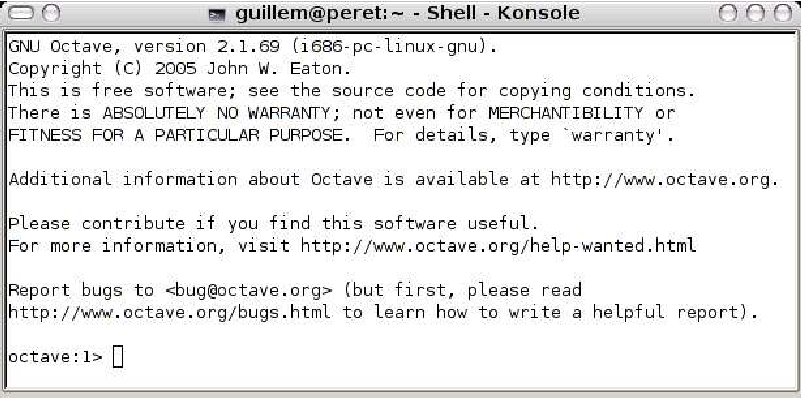
\includegraphics[%
  width=14cm,
  keepaspectratio]{figuras/octave}


  \caption{\label{cap:Esta-es-una}Esta es una consola Linux, mucho más
    útil que el Command Prompt de Windows}
\end{figure}


Si hacemos el esfuerzo de abstracción y simplificamos la ventana
anterior nos queda el símbolo de entrada:

\begin{verbatim}
>>
\end{verbatim}
¿Qué hacemos a parte de quedarnos paralizados? Pues si esto es una
calculadora vamos a usarlo como una calculadora:

\begin{verbatim}
>> 2+2
ans = 4
\end{verbatim}

Este ejemplo no sirve para nada pero resume perfectamente el uso de
Matlab. En el fondo es una calculadora programable con unas
posibilidades casi infinitas. Si a esto se suma un lenguaje intuitivo
y una gran biblioteca de funciones el resultado es una herramienta
verdaderamente útil para ingenieros y científicos.

Esta manera de trabajar no es un invento de Matlab, los lenguajes
interpretados ya existían mucho antes. Lo que sí es novedoso es basar
la arquitectura del lenguaje en conceptos matemáticos; entre ellos uno
muy importante: la función. Mientras los lenguajes clásicos se basan
en subrutinas o objetos Matlab dispone de una biblioteca formada
exclusivamente por funciones. Este diseño tan simple es lo que ha
llevado Matlab a su éxito, es un acercamiento matemático a la
programación orientada a matemáticas. Si queremos calcular el seno de
$\frac{\pi}{2}$ lo que haremos será llamar a la función como se haría
sobre el papel:

\begin{verbatim}
>> sin(pi/2)
ans = 1
\end{verbatim}
Entonces nada impide usar el mismo concepto para resolver problemas
mucho más complejos:

\begin{verbatim}
>> quad(@(x) besselj(2.5,x),0,4.5)
ans = 1.1178
\end{verbatim}
Acabamos de hacer la siguiente integral de la función real de Bessel
de primera especie:

$$\int_{0}^{4.5}J_{2.5}(x)dx$$

\texttt{quad} y \texttt{besselj} son funciones que se
han compuesto del mismo modo que se compondrían funciones matemáticas.
Esta línea de código puede ser incomprensible pero al final la
entenderemos con todos los detalles.


\section{El entorno de desarrollo Matlab.}

Matlab como programa no se limita a un intérprete en una consola, es
un entorno de desarrollo al completo. Al iniciar Matlab nos aparecerá
la ventana principal con la consola, el navegador de variables y el
historial de comandos (figura \ref{cap:Ventana-principal-Matlab})%
\footnote{En Unix Matlab puede funcionar también desde el intérprete
de comandos mediante la función \texttt{-nojvm}.  Es una opción interesante
cunando no hemos instalado ninguna máquina virtual de Java}. Evidentemente
lo más importante es la consola; todo lo demás, aunque útil, es prescindible.


\begin{figure}[h]
  \centering{}

  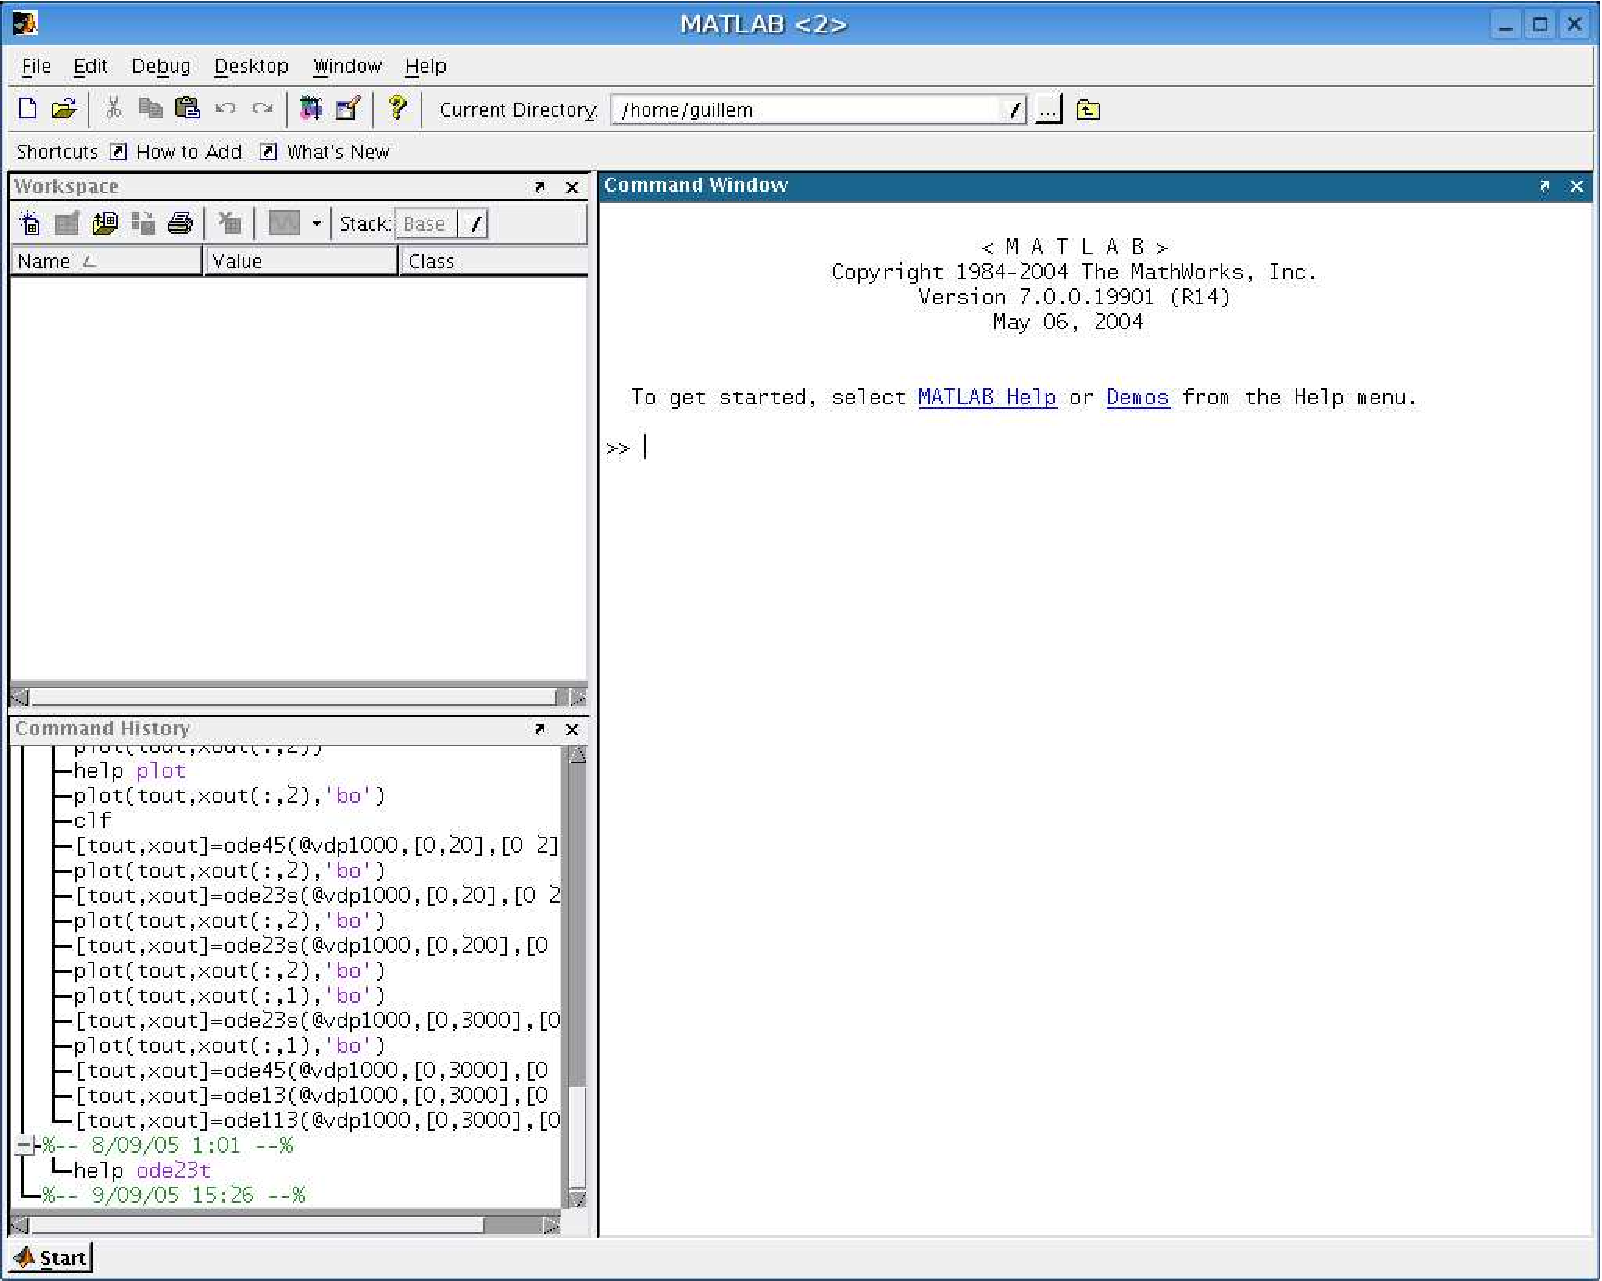
\includegraphics[ width=1\textwidth,
  keepaspectratio]{figuras/matlabenv}


  \caption{\label{cap:Ventana-principal-Matlab}Ventana principal de
    Matlab}
\end{figure}

La ventana principal no es más que la consola con algunas herramientas
adicionales. Para completar un entorno de desarrollo son necesarios
dos elementos más: un editor y un navegador de ayuda. El primero
aparece cuando editamos un archivo \texttt{.m} desde el gestor de
archivos o cuando creamos uno nuevo desde la ventana principal. Su
función es facilitar la creación de archivos de código Matlab y para
ello cuenta con {}``Syntax Highlighting'', tabulado automático,
soporte gráfico para debugging...

%
\begin{figure}[H]
  \centering{}

  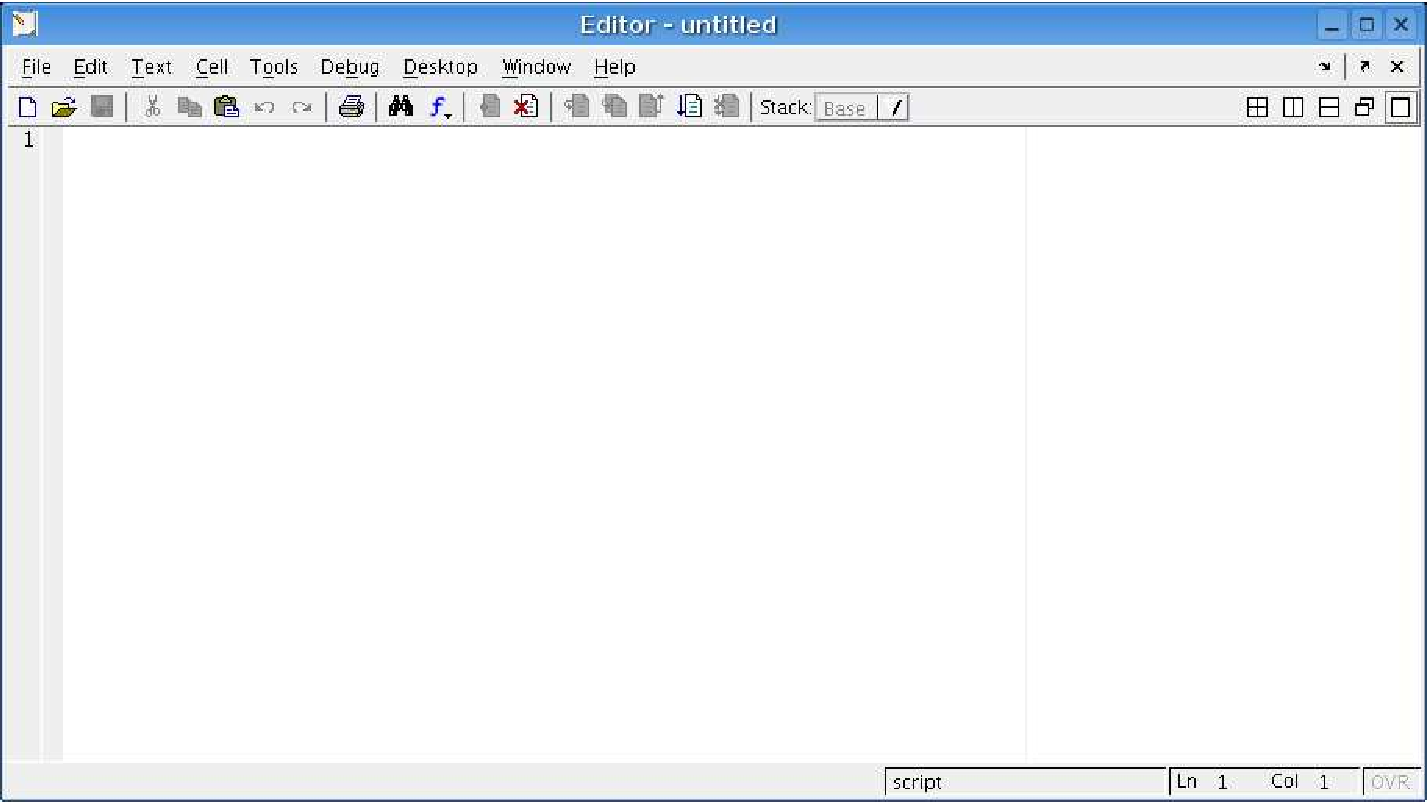
\includegraphics[%
  width=1\textwidth,
  keepaspectratio]{figuras/matlabed}


  \caption{\label{cap:Editor-Matlab}El editor de Matlab}
\end{figure}


Es muy importante llegar a dominar todas las posibilidades del editor.
Cuanto mejor lo conozcamos más fácilmente y rápidamente programaremos.

Finalmente el navegador de ayuda. Además de ser el mejor sitio donde
buscar ayuda puntual sus tutorías nos servirán para perfeccionar
nuestra habilidad con el lenguaje y el entorno. Podemos acceder a
él desde el menú {}``\texttt{Help}'' o mediante el icono con el
símbolo interrogante en la barra de herramientas.

%
\begin{figure}[h]
  \centering{}

  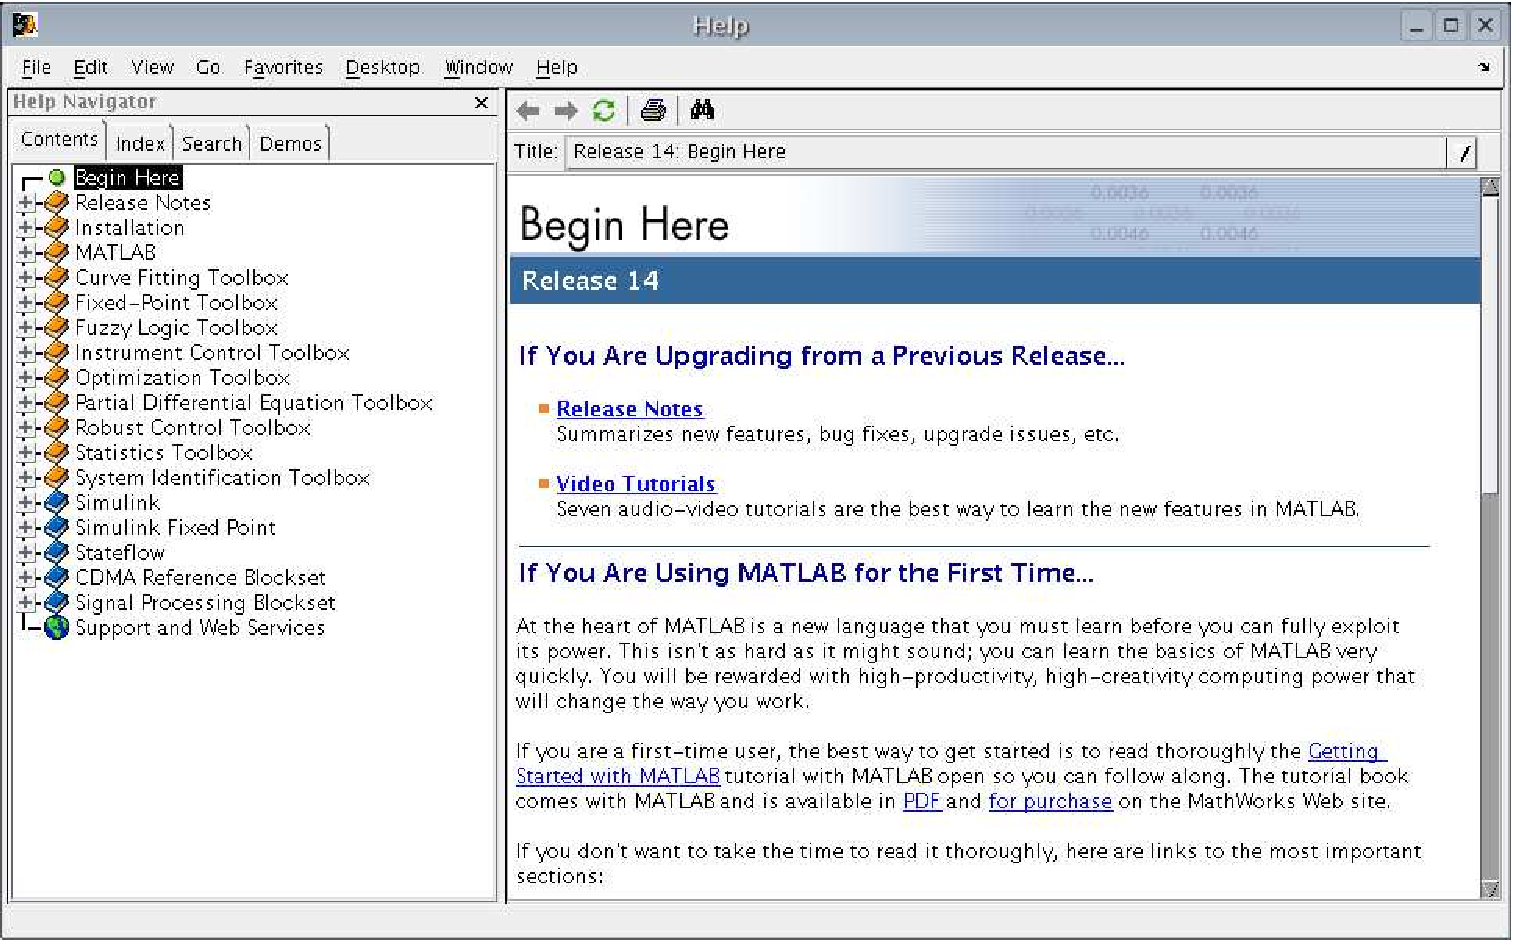
\includegraphics[%
  width=1\textwidth,
  keepaspectratio]{figuras/matlabhlp}


  \caption{\label{cap:Navegador-de-ayuda}Navegador de ayuda de Matlab}
\end{figure}



\section{Octave\index{Octave}}

Octave es también un lenuaje de scripting científico.  Aunque su
nacimiento nada tiene que ver con Matlab ha ido convergiendo hacia la
compatibilidad. Octave fue pensado como aplicación para la consola
UNIX. No tiene interfaz gráfica propia, navegador de ayuda, visor de
variables, editor, debugger...  Se puede decir que no tiene nada de
nada. Es un intérprete muy estable, ligero y orientado a programadores
más experimentados.

Octave es Software Libre soportado por una comunidad de
desarrolladores sin ánimo de lucro. Es un proyecto en colaboración
cuyos miembros nos prestarán ayuda cuando la solicitemos. Sus listas
de correo son públicas y son una gran fuente de información. Formar
parte del desarrollo de Octave es la mejor manera de conocer Matlab en
profundidad.

El lenguaje Octave es un poco más potente y mejor diseñado, si no nos
importa sacrificar la compatibilidad tendremos un poco más de libertad
programando.  Como parte del proyecto GNU su integración en un entorno
GNU/Linux es excelente; es por ello que se comunica perfectamente con
otros lenguajes de programación.  Puede ser una buena excusa para
perfeccionar o utilizar nuestros conocimientos de C++ o para
profundizar en UNIX.

Tampoco es verdad que Octave sea tan minimista. Existen esfuerzos para
dotar a Octave de más y más herramientas fuera del paquete oficial.
El más relevante es sin duda Octave-forge. Cualquiera que eche de
menos una función en Octave puede escribirla y mandarla al proyecto;
si lo creen conveniente la incorporarán en la próxima versión de la
colección. Además Octave-forge es un gran directorio de código
escrito. Puede servirnos para aprender como escribir una función como
es debido o como implementar algoritmos especialmente complejos. La
calidad de las funciones es variable pero la media es muy alta.

Otro proyecto interesante Octave Workshop de Sébastien Loisel.  Se
trata de una interfaz gráfica a la Matlab para Octave, orientada sobre
todo hacia usuarios de Windows.  Es un proyecto muy joven pero
prometedor; desde el principio ha apostado por una solución integrada.
Llena un vacío muy importante, de otro modo la curva de aprendizaje se
alarga por la necesidad de aprender a utilizar herramientas de UNIX en
un entorno Windows.

\subsection{El entorno de desarrollo Octave}

Cuando hemos hablado del entorno de desarrollo de Matlab han aparecido
tres ingredientes básicos: la consola, el editor y el naveador de
ayuda.  Como aplicación para la consola UNIX debemos confiar en las
herramientas propias del sistema: un editor polivalente como emacs o
vim, páginas de ayuda en formato info...  Aunque todas las piezas de
este entorno existen en Windows carecen de la misma integración con el
sistema operativo.  En este caso optaremos por un entorno de
desarrollo integrado como Octave Workshop.

El editor que mejor se complementa con Octave es Emacs (figura
\ref{cap:Emacs-editando-un}), parte esencial del proyecto GNU. Emacs
cuenta con un plugin para adecuarlo a la edición de archivos
\texttt{.m} y la comunicación con el intérprete Octave. Si no nos
sentimos cómodos con él siempre podemos optar por otros editores como
VIM o SciTe, este último muy adecuado para los usuarios de Windows.

El programa más utilizado para dar soporte gráfico a Octave es
GNUPlot.  Sus funcionalidades no son comparables a las ofrecidas por
Matlab pero son suficientes. Desde hace bastante tiempo se busca un
sustituto pero aún no ha aparecido ningún candidato adecuado.
Probablemente nuestra instalación de Octave incorpore GnuPlot, si no
es así tendremos que instalarlo puesto que es un requerimiento casi
indispensable.

Sobre el navegador de ayuda es muy conveniente obtener el directorio
de Octave-forge\index{Octave-forge}. Es un documento HTML comprimido
que cualquier navegador puede mostrar. No se acerca a las
posibilidades de la ayuda de Matlab pero es una buena herramienta de
consulta. En compensación, la ayuda interactiva de las funciones de
Octave suele ser de mayor calidad gracias al uso del formato
\emph{texinfo.}

%
\begin{figure}[h]
  \centering{}

  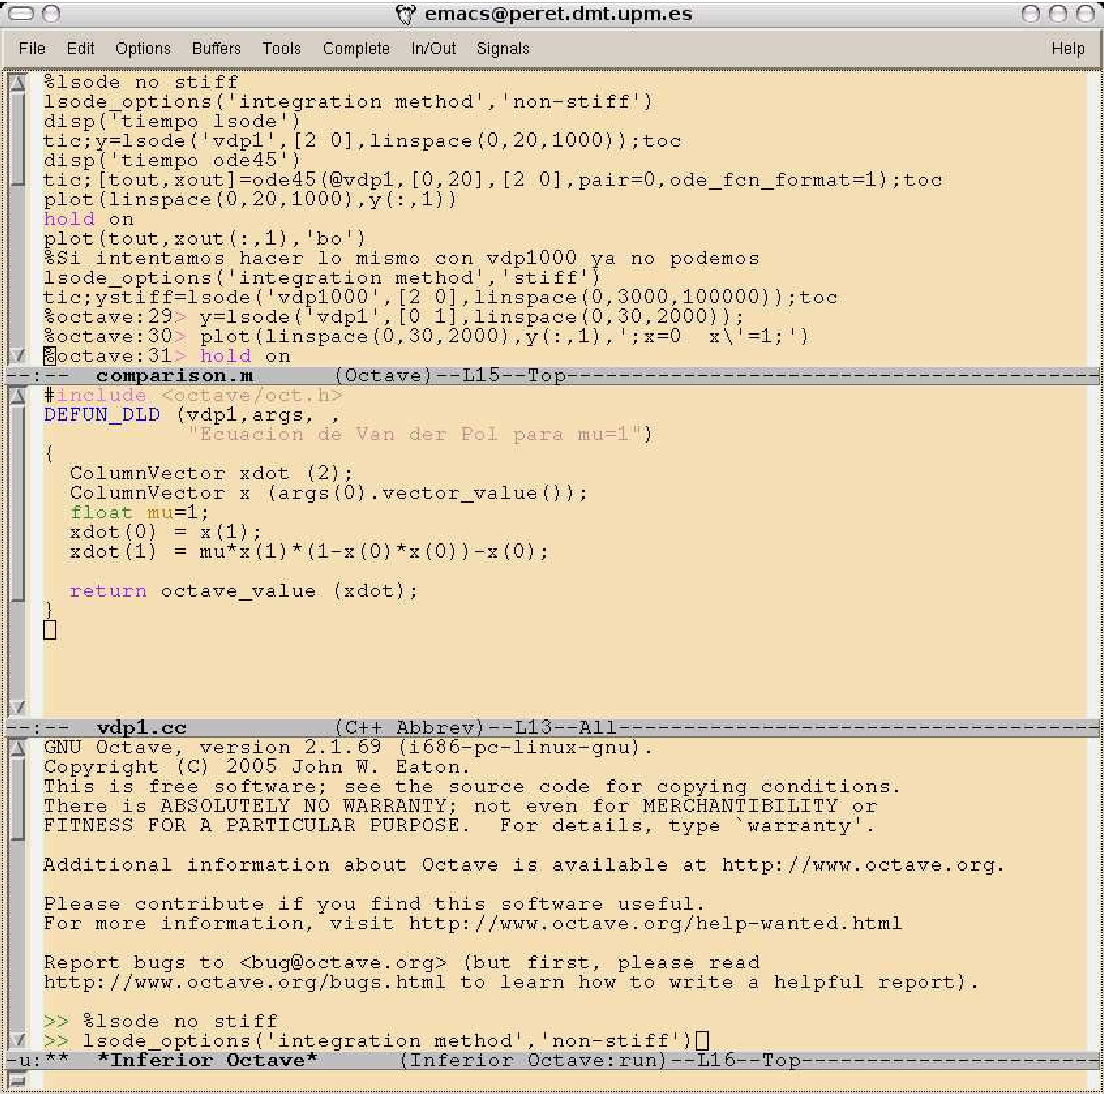
\includegraphics[%
  width=1\textwidth,
  keepaspectratio]{figuras/emacs}


  \caption{\label{cap:Emacs-editando-un}Emacs editando un archivo
    matlab, uno en C++ y debugeando simultáneamente.}
\end{figure}



\section{Los proyectos de software y los lenguajes de programación}

Cuando afrontamos un proyecto de sofware, sea del tipo que sea, la
primera consideración que se hace es la elección de la herramienta de
trabajo. En este caso un lenguaje de programación. Actualmente existen
un centenar de ellos y la elección no es sencilla.

¿Cuáles son los criterios principales?

\begin{itemize}
\item Que todos los miembros del proyecto dominen o conozcan el
  lenguaje.
\item El acceso a todas las herramientas necesarias.
\item El tiempo total de desarrollo del proyecto.
\item La calidad del resultado final.
\item La relación esfuerzo resultado.
\end{itemize}

Aunque estas condiciones parecen obvias no siempre han sido las
mismas.  Durante las décadas de los 70 y 80 programar se consideraba
una tarea laboriosa y complicada en la que no debía ahorrarse horas de
trabajo.  Que un ingeniero pasara miles de horas sentado delante de un
ordenador no se consideraba tiempo malgastado.  Existía la creencia de
que ninguna tecnología era capaz de competir con la pericia y que
cualquier aumento en el rendimiento compensaba con creces el tiempo
dedicado.

Durante los 90 aparecieron multitud de herramientas orientadas a
aumentar la productividad y con ellas un cambio esencial de filosofía.
El criterio era mucho más pragmático: todo cuenta.  Debemos valorar el
tiempo total de desarrollo, la calidad del código escrito, la
portabilidad del programa...  Ya no era sólo el programador y su
programa, se había convertido en una pieza dentro de una gran
maquinaria fuera consciente de ello o no.  La aparición de los
lenguajes interpretados acentuó aún más esta concepción.  Tareas que
antes llevaban días podían hacerse en horas y cada vez se hacía menos
necesario un conocimiento preciso de informática para programar.

El criterio esencial pasó de ser la calidad del resultado final a ser
la relación esfuerzo por resultado.  Los lenguajes interpretados suelen
mejorar dicha relación gracias a simplificar la metodología de
trabajo.

Hemos hablado de la distinción entre lenguajes de código fuente o
compilados y los lenguajes interpretados pero no hemos tratado sus
diferencias en el uso. Un lenguaje interpretado elimina la
necesidad del ciclo escritura-compilado-debugging.


\subsection{El ciclo de desarrollo clásico}

Todas las herramientas de desarrollo de sofware en general intentan
paliar los problemas derivados de este ciclo. Cuando programamos con
un lenguaje compilado como C o Fortran nos vemos obligados a convertir
el código fuente en un programa, ejecutar el programa, analizar el
resultado y, en el caso que sea necesario, realizar un debugging.  El
debugging es el proceso de depuración en tiempo de ejecución. Un
programa compilado se ejecuta entero y escupe un resultado final; si
no es el esperado y el código parece correcto nos veremos obligados a
analizar los resultados intermedios. ¿Cómo puede hacerse eso en un
ejecutable que parece un bloque monolítico? Introduciendo pausas en la
ejecución llamadas \emph{breakpoints} que paran el hilo para comprobar
los resultados intermedios.

Este ciclo es rentable sólo en el caso de grandes aplicaciones muy
integradas con las librerías o que requieren una máxima optimización.
¿Qué sucede si nuestra aplicación busca simple y llanamente un
resultado después de un tiempo de desarrollo lo más corto posible?
Entonces sacrificaremos los lenguajes de programación {}``clásicos''
en favor de los lenguajes interpretados


\subsection{Rapid Application Development o RAD}

La ventaja de los lenguajes interpretados respecto a los compilados es
evidente, uno de los pasos del ciclo de desarrollo, la compilación,
desaparece y el debugging es trivial. Esta diferencia que puede
parecer irrisoria suele condicionar enteramente el proceso.

Los lenguajes de scripting nacieron como una manera sencilla de hacer
tareas complejas o repetitivas. Por ejemplo, tenemos en un directorio
cualquiera medio centenar de archivos de los que no conocemos el nombre.
Nuestro objetivo es añadir al final de todos los que contengan la
combinación de letras \emph{abc} el símbolo \texttt{\_}. Realizar
manualmente esta tarea puede requerir unos cuantos minutos pero si
disponemos de un intérprete de \emph{python} en el sistema lo
conseguiremos con:

  \begin{verbatim}
>>> import os
>>> for file in os.listdir('.'):
...     if file.find('abc') >= 0:
...         os.system('mv %s %s%s' %(file,file,'_'))
\end{verbatim}
Parece fácil. ¿Verdad? Si para los administradores de sistemas
conocer un lenguaje interpretado de propósito general es así de útil
¿Por qué no iba a serlo para un ingeniero? ¿Cuántas líneas de código
serían necesarias para programar lo mismo en C o Fortran?

Los ordenadores incrementan exponencialmente su potencia y cada año
los lenguajes interpretados son más y mas competitivos; ahora se usan
para casi cualquier aplicación y han obligado a todo el mundo a
cambiar su punto de vista. Los lenguajes interpretados se utilizaban
únicamente cuando se quería una interacción directa con el usuario,
una manera de extender las capacidades de un programa que estaba
escrito en un lenguaje compilado. Ahora podemos utilizar lenguajes
interpretados para aplicaciones de alto coste computacional y
pasaremos a un programa puramente compilado sólo en caso de necesidad.

Las aplicaciones de simulación suelen ser programas no muy largos que
pueden o no solicitar una optimización máxima. En cualquiera de los
dos casos se utilizará un lenguaje interpretado porque nuestro
objetivo es el RAD o Rapid Application Development. En programas
cortos porque es el único modo de acortar el tiempo de desarrollo y en
los largos para la fase de prototipado.

Para que un lenguaje interpretado pueda ser utilizado como una
herramienta de RAD debe cumplir los siguientes requisitos:

\begin{enumerate}
\item Debe ser lo suficientemente polivalente como no necesitar acudir
  a otros lenguajes de programación durante del proceso de diseño.
\item Debe poner a nuestra disposición suficientes herramientas como
  para que no sea necesario \emph{buscar}.
\item Debe formar parte de un entorno de desarrollo cómodo y versátil
  y sencillo.
\item Su sintaxis debe ser clara para que el código sea leíble. En la
  mayoría de los casos los códigos se reciclan y mutan en el tiempo.
  Si cada vez que cambia de manos requiere ser leído cinco o seis
  veces para saber qué está haciendo es cualquier cosa menos rápido.
\end{enumerate}
Matlab cumple sobradamente todos estos requisitos. El lenguaje es
sencillo, cómodo y leíble; las bibliotecas de funciones son enormes y
siempre que no nos salgamos del cálculo numérico no tenemos que acudir
a otros lenguajes de programación.


\subsection{Otros lenguajes orientados a RAD.}

Matlab tiene competencia, esperada e inesperada. La esperada viene de
programas comerciales como Mathematica o Scilab. Además Mathematica
concepto un concepto interesante conocido como Notebook, ya
introducido por Maple, para potenciar las sesiones interactivas. Lo
que probablemente no esperaban los desarrolladores de Matlab es que la
competencia les llegara por parte de los lenguajes interpretados de
propósito general.

Si nos obligamos a mantener el sentido crítico aplicado a las
herramientas debemos tener en cuenta lenguajes como Python o Ruby,
sobre todo Python gracias al proyecto SciPy. De momento son opciones
poco consolidadas pero puede que en un futuro sean una referencia en
el desarrollo de aplicaciones de simulación.

\section{Una visión contemporánea del desarrollo de aplicaciones de
simulación}

Es muy común que un ingeniero o un científico tenga que programar a
menudo. El desarrollo de aplicaciones de software está ligado a la
necesidad de simular un sistema de cualquier tipo. En la mayoría de
los casos los programadores son ingenieros, matemáticos o físicos sin
una formación teórica en lenguajes de programación. La mayoría de
ellos son autodidactas sin conocimientos específicos sobre metodología
y práctica de la programación. En muchos casos se construyen programas
deficientes con herramientas inadecuadas y del peor modo posible.  No
se usan bien los editores, los debuggers brillan por su ausencia, no
se aplican las metodologías orientadas a la programación sin errores...

La raíz de estos problemas es que el jefe del proyecto es el primero
en desconocer el entorno ideal. Casi siempre existen carencias en el
diseño de la aplicación y en la elección de las herramientas. ¿Cuántos
ingenieros han oído hablar del UML%
\footnote{UML son las siglas del Universal Modelling Language. Es un
  \emph{estándar} para la creación de diagramas que modelan la
  estructura de cualquier cosa, aunque fueron pensados para sistemas
  altamente lógicos como los programas de ordenador.%
}? ¿Y de la refactorización? ¿Cuántas aplicaciones de simulación están
escritas con un lenguaje orientado a objetos? ¿Y en un lenguaje
interpretado?  \emph{Los ingenieros somos tan soberbios como
  todoterrenos. Somos tan capaces de arreglar cualquier cosa como
  incapaces de reconocer que un mejor diseño nos ahorraría muchos
  quebraderos de cabeza}. En programas que requieren desarrollos de
horas o de días el coste de empezar de cero por culpa de un mal diseño
no es ningún problema; medida que los tiempos de desarrollo crece las
situación se vuelve más y más crítica.


\subsection{Errores típicos}

El ingeniero tipo escribe un código lamentable, ilegible.
\textbf{Si en la construcción del ala de un
avión no se puede hacer una chapuza... ¿Por qué puede serlo el código
del programa que simula su inestabilidad?} ¿Porque funciona? Otra
consideración fundamental es que si queremos producir una pieza
especialmente complicada construiremos antes un prototipo para saber
si cumple con los requisitos funcionales.  Si aplicáramos los mismos
principios al desarrollo de simulaciones sería intolerable ponerse a
escribir en Fortran más de 2000 líneas de código sin haber probado
antes el algoritmo en Matlab. Esta práctica es tan poco común en la
empresa como en el ámbito científico.

Otro error es el de subestimar el tiempo de desarrollo. Un programa de
simulación decente, con requerimientos computacionales medios o
grandes, puede desarrollarse en uno o dos años. Lo que suele hacerse
es tomar un lenguaje lo más rápido posible para minimizar el tiempo de
cálculo. Los lenguajes rápidos son principalmente dos, C y Fortran.
Normalmente se trabaja sin diseño, sin prototipos... Los errores
incomprensibles pueden alargar la aparición del primer ejecutable en
un 50\% del tiempo del proyecto, mucho más que lo que ahorraríamos en
el tiempo de ejecución.

Quizás la peor práctica de todas es la de no documentar el código a
medida que se escribe. Un código sin documentación o uno sin una
documentación adecuada puede ser un infierno hasta para uno mismo.  Si
leemos código escrito por nosotros mismos un año antes es como si lo
hubiera escrito alguien que no conocemos de nada. ¡Esto sucede de
verdad! Os lo digo por mi propia experiencia. Los comentarios son muy
útiles, hay que comentar cualquier estructura que no tenga una lógica
aplastante y escribir código obvio no es tan fácil como parece.


\subsection{¿Cuál es entonces el espacio de Matlab?}

Matlab es absolutamente superior en aplicaciones cortas y sencillas.
Reduce la longitud del código y el tiempo de desarrollo
significativamente además de ser un lenguaje leíble, escalable%
\footnote{Se dice que un lenguaje es escalable cuando todas sus
  virtudes se mantienen independientemente de la longitud del
  programa. Matlab es escalable pero hasta un límite; en aplicaciones
  especialmente grandes empiezan los problemas de uso de memoria y de
  acumulación de archivos de función. Los lenguajes compilados son
  típicamente escalables y algunos lenguajes interpretados como java y
  python también escalan perfectamente.%
} y sencillo. Todas las herramientas necesarias están dentro de la
misma aplicación y la documentación está embebida en el propio
programa%
\footnote{La ayuda de Matlab es un ejemplo de cómo se debe documentar
  una colección de funciones.%
}. Es una opción interesante en el proceso de diseño (cuando existe) y
es esencial en el proceso de análisis de datos, mucho menos exigente
computacionalmente.

La mayoría de los programas que escribe un ingeniero son cortos, y
requieren casi siempre las mismas herramientas matemáticas (álgebra
lineal, representación de funciones, integración numérica...). Se
busca efectividad, rapidez y pocos errores. Matlab es el lenguaje de
programación y la aplicación que mejor encaja en todos estos
requisitos en lo que a ingeniería se refiere.


\subsection{¿Y el espacio de Octave?}

Supongamos que ya dominamos Matlab de un modo razonable.  Como es 

\subsection{Los lenguajes \emph{pegamento}}

Otra característica de los lenguajes interpretados es que ellos mismos
están construidos sobre lenguajes compilados. Matlab, por ejemplo,
está escrito casi enteramente en C, mientras que Octave lo está en
C++. Esto significa que pueden integrarse perfectamente con sus
lenguajes \emph{padre}. Es de sobra sabido que los lenguajes
interpretados son entre uno y dos órdenes de magnitud más lentos que
los compilados.  La solución es acoplarles rutinas escritas en algunos
lenguajes compilados como C, C++ o Fortran para conseguir un aumento
significativo de velocidad.  Matlab empezó como una colección de
subrutinas en Fortran que se acoplaban a un intérprete interactivo.

Si este proceso se realiza sistemáticamente durante el desarrollo se
dice que el lenguaje interpretado sirve de \emph{pegamento} entre las
unidades de programa. Se puede decir que se buscan las ventajas de los
dos planteamientos, nos acercamos a la velocidad del código
enteramente compilado mientras mantenemos la versatilidad de un
script.

Matlab es capaz de convertir código en C o Fortran en archivos tipo
\texttt{mex} y Octave cuenta con el programa \texttt{mkoctfile}
(sección \ref{sec:Extender-Octave-con}) que realiza una labor
parecida. Lenguajes más polivalentes como Python, Ruby o
Perl cuentan con mejores herramientas.

%Elementos del lenguaje Matlab

%%%%%%%%%%%%%%%%%%%%%%%%%%%%%%%%%%%%%%%%%%%%%%%%%%
\chapter{MATLAB}

%%%%%%%%%%%%%%%%%%%%%%%%%%%%%%%%%%%%%%%%%%%%%%%%%%


\section{El lenguaje y las bibliotecas}

Antes de entrar en materia es importante que sepamos qué diferencias
hay entre las sentencias de un lenguaje de programación y la
biblioteca de funciones.

Las sentencias son las palabras clave independientes. Esto significa
que si las eliminaremos del lenguaje no podríamos sustituirlas con
ninguna combinación del resto de sentencias del lenguaje. Esta
definición no es estricta; algunas palabras clave comunes se
consideran sentencias cuando se hace un uso muy frecuente de ellas.

El total de sentencias y de reglas de escritura son lo que forman el
lenguaje de programación descrito en un documento llamado
\emph{referencia\index{referencia}.}  Como Matlab es un programa
comercial no existe tal documento.

El resto de funciones y subrutinas son parte de la
\emph{biblioteca\index{biblioteca}}.  Son palabras clave que cumplen
una tarea y no pueden ser consideradas sentencias porque están
escritas con ellas. Algunas funciones de uso muy frecuente llegan a
ser parte del mismo lenguaje, el grupo que forman se llama
\emph{biblioteca estándar}\index{biblioteca estándar}.  El conjunto de
sentencias y biblioteca estándar se conoce como
\emph{especificaciones} y en el caso que el lenguaje tome vida propia,
es decir, sus especificaciones pasen a ser públicas; se llama
\emph{estándar}. Estos documentos existen para la mayoría de los
lenguajes de programación conocidos: C, C++, Ada, Fortran, Python...
Matlab no es uno de ellos.

Al ser un lenguaje sujeto a una herramienta Matlab es Matlab y punto;
sin embargo podemos aplicar estas definiciones estrictas para
acercarnos a él como lo haríamos con el resto de lenguajes. La
organización interna de Octave sigue este criterio. Se podría decir
que Octave es el conjunto de sentencias mas la biblioteca estándar y
que el resto de colecciones de funciones (y hay bastantes) son los
toolkits. La Compatibilidad entre los dos se sitúa sólo en las
sentencias aunque se extiende en gran manera con la biblioteca de
funciones. Por lo menos las funciones básicas son compatibles, casi
idénticas.

Matlab tiene muy pocas sentencias. Como lenguaje es muy sencillo
aunque cada versión incluye nuevas especificaciones. En los últimos
años se ha añadido la extensión para programación orientada a objetos
y el diseño de interfaces gráficas. Octave es ligeramente distinto en
su concepción; es más minimista y cuenta con muchas menos funciones
pero es más fácilmente extensible. Son las diferencias típicas entre
los productos libres y los comerciales.

Este capítulo es la referencia del lenguaje; en él veremos argumentos,
variables, operadores y sentencias que nos servirán para programar
funciones y scripts así como la arquitectura general del programa.  Es
con diferencia la parte más importante del libro y no se ha dividido
en varios capítulos para no romper el hilo conceptual.

\emph{Siempre que se hable exclusivamente de Matlab nos referiremos a
  las características comunes de Matlab y Octave. Cuando la palabra
  Matlab se utilice en una diferencia respecto a Octave nos estaremos
  refiriendo al programa comercial. Por sencillez no se ha
  diferenciado tipográficamente la palabra Matlab en los dos
  contextos.}


\section{Convenciones}

A partir de ahora escribiremos un comando escrito en la consola de la
siguiente manera:

\begin{verbatim}
>> %Esto es un comentario puesto en la consola de Matlab
\end{verbatim}
Escribiremos todas las palabras clave con letra de formato fijo como
esta función: \texttt{sin(x)}.

Veremos que la sintaxis de Matlab no es muy distinta de la de
cualquier otro lenguaje; las diferencias serán las de siempre, los
símbolos de continuación, los comentarios... Aunque sea un poco
temprano los listamos a continuación:

\begin{description}
\item [\texttt{'\_'}]Comillas simples. Sirven para introducir texto
  literal, todo lo que se encuentre en este entorno será tomado como
  texto y no como el nombre de una variable
\item [\texttt{{}``\_''}]Comillas dobles. Símbolo de carácter también
  soportado en Octave.
\item [\texttt{\%}]Porcentaje. Es el símbolo del comentario. Todo lo
  que está por detrás de este símbolo en una línea es ignorado por el
  intérprete.
\item [\texttt{\#}]Almohadilla. Símbolo del comentario sólo soportado
  por Octave. Es muy útil cuando se quieren añadir comentarios en la
  cabecera de una función sin que el parser\index{parser}%
  \footnote{Todos los lenguajes interpretados procesan el código con
    una herramienta llamada parser. El parser lee cada línea y
    distingue las palabras clave, las variables y los argumentos para
    que el intérprete pueda hacer su trabajo sin problemas.%
  } lo tome como parte de la ayuda.
\item [\texttt{...}]Tres puntos. Al añadir alguno de estos dos
  símbolos al final de una línea significa que se tomará la posterior
  como continuación
\item [\texttt{\textbackslash{}}]Barra invertida. El símbolo de
  continuación de C, C++ y Python también está soportado en Octave.
\item [\texttt{;}]Punto y coma. Símbolo de retorno de carro. Sirve
  para concatenar más de una sentencia en la misma línea y para
  inhibir la salida por consola del resultado.
\item [Importante:]El punto y coma al final de una sentencia explicita
  el retorno de carro e inhibe que salga el resultado por pantalla.
\end{description}

\subsection{Operaciones elementales con Matlab}

Las convenciones para las operaciones en Matlab son idénticas que en
cualquier otro lenguaje de programación o que en una calculadora
programable. El orden de asociación de las operaciones es también el
mismo. Primero se operan las funciones matemáticas elementales (senos,
cosenos, logaritmos...), las multiplicaciones y divisiones y luego
sumas y restas. Por ejemplo, para realizar la siguiente operación:
$$\frac{1}{\frac{2}{0.1^{1/2}}-\frac{0.4}{2^{1/3}}}$$
introduciremos enla consola:

\begin{verbatim}
>> 1/((2/0.1 ^(1/2))-(0.4/2 ^(1/3)))
\end{verbatim}

Evidentemente Matlab no distingue entre elementos numéricos y
variables, la ecuación:
$$\frac{a}{\frac{b}{c{}^{d}}-\frac{e}{g^{f}}}$$
\begin{verbatim}
>> a/(b/c^d-e/g^f)
\end{verbatim}

Los paréntesis sirven para variar el orden normal de las operaciones a
realizar.


\subsection{Algunas palabras clave y atajos de teclado.}

La consola es un entorno de trabajo más potente de lo que parece.
Editar directamente en ella es un ejercicio cómodo gracias a una serie
de atajos de teclado de gran utilidad. Uno de los más potentes es la
capacidad de auto-completar alguna palabra clave con la tecla de
tabular, tab completion en inglés. Por ejemplo, si nos encontramos en
el intérprete Octave y nos acordamos cómo se escribe exactamente la
función para trasponer una matriz podemos hacer lo siguiente,
escribimos sólo el inicio de la palabra y luego presionamos la tecla
de tabular:

\begin{verbatim}
>> tra<TAB>
trace      transpose  trapz
\end{verbatim}

Esta es una característica común de casi todas las consolas
existentes, ya sea una consola de UNIX o el Command Prompt de Windows.
La consola gráfica de Matlab es un poco más potente gracias a su
interfaz (figura \ref{cap:Tab-completion-en}):

%
\begin{figure}[h]
  \centering{}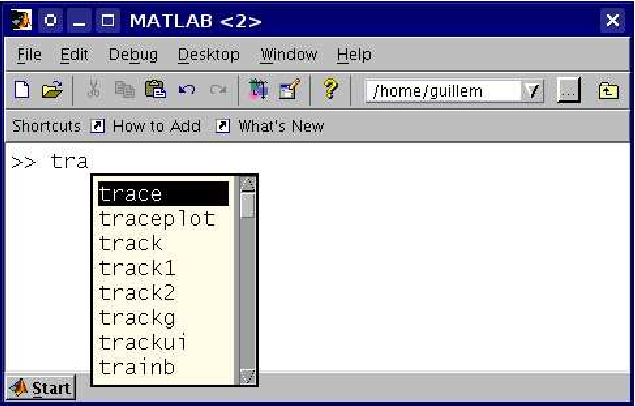
\includegraphics[width=8cm,
  keepaspectratio]{figuras/autocompletion}


  \caption{\label{cap:Tab-completion-en}Tab completion en Matlab}
\end{figure}


A continuación una lista de palabras clave y atajos de teclado que
pueden hacernos la vida mucho más fácil:

\begin{description}
\item [\texttt{exit}]Cierra el intérprete, equivalente a cerrar la
  ventana.
\item [\texttt{<CTRL>-c}]Corta la ejecución del comando actual (kill)
\item [$\uparrow$]Reescribe líneas anteriores. A medida que
  presionemos este carácter aparecerán en la línea actual todos los
  comandos escritos anteriormente. Una vez estemos viendo los comandos
  podemos movernos entre ellos mediante los cursores.
\item [\texttt{<CTRL>+<$\rightarrow$,$\leftarrow$>}]Hace avanzar o
  retroceder el cursor por palabras en vez de por caracteres.
\item [\texttt{clc}]Limpia la pantalla del intérprete de comandos
\end{description}

\section{La Ayuda(I)}

La manera más fácil de acceder a la ayuda tanto en Matlab como en
Octave es mediante la consola y el comando \texttt{help}\index{help}.
Cada comando y función lleva consigo la información necesaria para que
conozcamos su uso y sus funcionalidades%
\footnote{Más adelante aprenderemos cómo introducir esta información a
  cualquier función que escribamos%
}. Para acceder a la ayuda de una función teclearemos

\begin{verbatim}
>> help  {nombre de la función}
\end{verbatim}

Esto significa que debemos saber cómo se llama la función. Si
introducimos \texttt{help} sin ningún argumento nos aparecerá una
ayuda general desde donde podremos encontrar cualquiera de las
funciones disponibles.

Uno comando bastante útil cuando trabajamos desde una consola o por
red es \texttt{more}\index{more}. Si activamos el comando con
\texttt{more on} activaremos el paginador de modo que cuando el texto
que aparezca en pantalla se salga de la misma interrumpirá el texto
hasta que nosotros le pidamos que continúe. Esto evita el
comportamiento tan desagradable que tienen las ayudas especialmente
largas en las que siempre tenemos que utilizar la barra de
desplazamiento para ver el principio. Para salir del texto sin tener
que desplazarnos hasta el final pulsaremos la tecla \texttt{<Q>}.


\section{Tipos de archivos en Matlab}

Al igual que el intérprete es capaz de entender comandos mediante su
consola interactiva, también es capaz de leer archivos de código o
scripts. En el caso de Matlab los archivos asignados al intérprete
son los que terminan con la extensión \texttt{.m}. Pero para entender
cómo estos archivos interactúan con el intérprete es necesario 
que entendamos la arquitectura interna de Matlab.

Gran parte de la funcionalidad de Matlab se basa en su biblioteca de
funciones.  Una función en Matlab es equivalente a una función
matemática; es una tarea encapsulada que puede depender de una o
varias variables.  Matlab tiene una extensísima biblioteca de funciones, 
la mayoría de ellas son archivos con la extensión \texttt{.m} que
lee el intérprete.  Pero el intérprete no puede saber por ciencia infusa
dónde se encuentran dichas funciones.  Si en la consola introducimos:
\begin{verbatim}
>> sin(x)
\end{verbatim}
¿Cómo sabe Matlab dónde se encuentra la función seno?  La respuesta es
que Matlab ya sabe en qué directorios del sistema puede encontrar
archivos \texttt{.m} desde su instalación.

¿Significa esto que si creamos nuestras funciones debemos guardarlas
en estos directorios?  Ni mucho menos.  Matlab cuenta con un directorio
especial en el que también busca funciones; es el llamado \emph{directorio
de trabajo}.  Si estamos utilizando la interfaz gráfica de Matlab lo
seleccionaremos en la barra de herramientas.  Si en cambio accedemos 
a Matlab por consola o optamos por Octave el directorio de trabajo
será el directorio actual (en UNIX el contenido en la variable de
sistema PWD).  Cada vez que se invoque una función en Matlab buscará
en los directorios habituales y en el directorio de trabajo.

\subsection{Funciones(I)\label{sub:Funciones(I)}}

Una función\index{función} es una \emph{unidad de programa}, una tarea
independiente que puede o no depender de variables externas.  Las unidades
de programa típicas son las funciones, las subrutinas, las clases...
Matlab basa toda su potencia y su sencillez en el constante uso de
funciones.  La razón es bien sencilla; si Matlab es un programa para
cálculo numérico es normal que la unidad de programa esencial sea
la que tiene un significado más matemático

En Matlab se define una función del siguiente modo:\footnote{El comando
  \texttt{end} sólo es necesario en Octave cuando queremos acoplar
  funciones en los scripts o más de una función en un mismo archivo.
  En Matlab no es necesario porque cada función está asociada a un
  único archivo, el final del mismo hace de texttt{end}.}:

\begin{verbatim}
function [variables_de_salida]= nombre(variables_de_entrada)
  Comandos que terminamos asignando a las variables de salida
{end}
\end{verbatim}
 
Por ejemplo,si queremos implementar una función que sume dos escalares 
debemos hacer lo siguiente:

\begin{verbatim}
function [c]=suma(a,b)
  c=a+b;
\end{verbatim}

Y lo guardaremos en un archivo que se llame igual que la función; en
el caso del ejemplo será \texttt{suma.m}. Luego lo guardaremos en nuestro
directorio de trabajo.

El concepto de función va más allá pero esta descripción es suficiente
para entender su papel dentro de la arquitectura de Matlab.


\subsection{Scripts}

Los scripts hacen la función de un programa completo, su hilo de
sentencias tiene un principio y un final y no necesita actuar con
ninguna variable externa al código. La diferencia entre un
script\index{script} y un archivo de código fuente es que el script es
una transcripción literal de comandos de consola; se dice que es
\emph{secuencial}.  Esto no nos permite explotar las posibilidades de
los formatos libres ni utilizar secuencias de control tipo
\texttt{goto}%
\footnote{Mejor, porque este tipo de estructuras no son nada
  aconsejables.%
}. También tienen la extensión \texttt{.m} y se pueden ejecutar de
varios modos:

\begin{itemize}
\item Dentro del intérprete. Si hemos guardado el archivo en alguno de
  los directorios de búsqueda de funciones el intérprete ejecutará
  toda la secuencia de comandos introduciéndole el nombre del script
\end{itemize}
\begin{verbatim}
>> nombre_del_archivo
\end{verbatim}
\begin{itemize}
\item Fuera del intérprete. Dentro de una consola llamando el
  intérprete con el nombre de archivo como argumento. Por ejemplo, en
  una consola cualquiera:
\end{itemize}
\begin{verbatim}
$> matlab nombre_del_archivo
\end{verbatim}

Podemos llamar a funciones en nuestros scripts siempre que sea con
variables que hayamos inicializado antes de la llamada. El concepto es
el mismo, no es más que la transcripción de los comandos que se
introducirían en la consola.


\subsection{Nuestra primera función}

En esta primera función no usaremos ninguno de los elementos
característicos de la programación en Matlab. Estos son los que
encontramos en cualquier código de simulación: contadores, funciones
elementales, condicionales, casos... Empezaremos con el archivo
\texttt{aprsin.m}, que es la aproximación de orden 3 del desarrollo de
Taylor en 0 de la función seno. Para ello editamos el archivo nuevo de
nombre \texttt{aprsin.m} en el directorio que nos diga Matlab o Octave
según el caso y pondremos en ella lo siguiente:

\begin{verbatim}
function out=aprsin(x)
  out=x-x^3/6;
\end{verbatim}

Vemos que asignamos a la variable \texttt{out} las operaciones
que hacemos sobre la variable de entrada \texttt{x}. La idea es
mantener las características de una función matemática. Una vez la
hayamos guardado en el directorio de trabajo esta función puede ser llamada
por el intérprete de Matlab o por cualquier script.
Para probarlo nos vamos a la consola y tecleamos:

\begin{verbatim}
>> y=aprsin(1.3)
\end{verbatim}
que debe darnos como resultado:

\begin{verbatim}
y = 0.93383
\end{verbatim}
Aún es pronto para algunos conceptos, hay que aclarar un par de
cuestiones:

\begin{itemize}
\item Las variables \texttt{x} y \texttt{out} son de uso interno de la
  función.  Desde la consola o desde un script podemos usar las
  variables que queramos. Esta abstracción es común en todos los
  lenguajes de programación; la entenderemos cuando hablemos de la
  diferencia entre variable y argumento.
\item El punto y coma significa lo mismo que el retorno de carro.
  Tenemos que recordar siempre que la diferencia entre hacer un
  retorno de carro y poner el punto y coma es que en el segundo caso
  el programa no nos da ningún output. Llenaremos siempre las
  funciones de puntos y comas para no recibir resultados intermedios
  inútiles.
\end{itemize}

\subsection{Nuestro primer script}

Vamos a comparar nuestra aproximación de la función seno con la
función exacta y lo vamos a escribir en un guión. Para ello creamos el
archivo \texttt{comparar.m} y escribimos lo siguiente en él:

\begin{verbatim}
x=linspace(-pi,+pi,100);
for i=1:100
    y(i)=aprsin(x(i));
end
plot(x,[y;sin(x)])
\end{verbatim}
Para ejecutarlo vamos a la consola y tecleamos:

\begin{verbatim}
>> comparar
\end{verbatim}
E inmediatamente va a aparecer la figura \ref{cap:figura-ejemplo1}:


\begin{figure}[h]
  \centering{}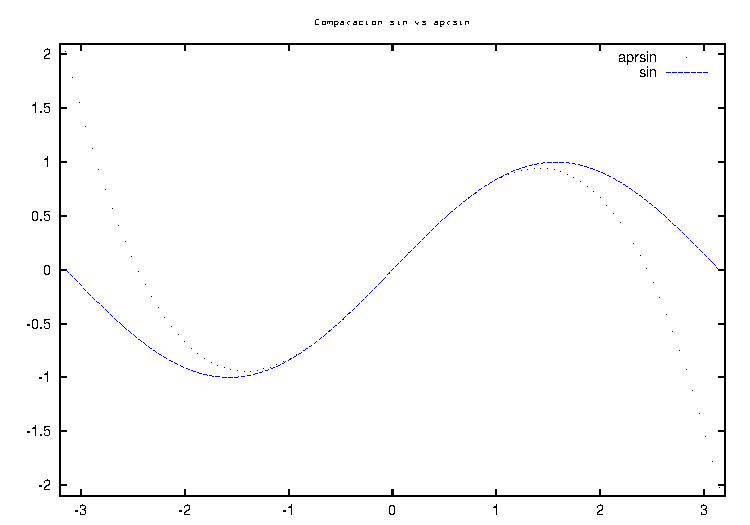
\includegraphics[%
  width=12cm,
  keepaspectratio]{figuras/figuraejemplo1}


  \caption{\label{cap:figura-ejemplo1}Comparación del desarrollo de
    Taylor}
\end{figure}


Aún es temprano para entender exactamente qué hace el script, lo
iremos viendo paso a paso; pero ha servido para ver cuál es la
relación entre funciones, los scripts y Matlab.


\subsection{Una gran diferencia entre Matlab y Octave}

\emph{Matlab no puede definir funciones directamente en el intérprete
o en un script.  Cualquier función debe ser un archivo independiente
por simple que esta sea}. Por ejemplo, si en Matlab escribimos:

\begin{verbatim}
>> function c=suma(a,b)
??? function c=suma(a,b)
    |
Error: Function definitions are not permitted at the prompt or in scripts.
\end{verbatim}
Recibimos un error.  En cambio Octave puede definir funciones tanto
en el intérprete como en un script, algo que dota a este intérprete
alternativo de algo más de versatilidad.

Éste es uno de los grandes puntos débiles de Matlab. Ignoro
el hecho por el que aún no lo soportan.

Lo que no se puede hacer ni en Matlab ni en Octave es poner varias
funciones en un mismo archivo de función. No es muy difícil ver por
qué. El lenguaje Matlab, cuando llama a una función, busca por los
directorios algún archivo que se llame como la función, y luego busca
una sentencia ejecutable en él. Esto implica que cada archivo sólo
puede contener una cabecera%
\footnote{Puede contener más funciones pero sólo se puede llamar una.
  Esta es la función que tenga la cabecera en la primera linea cuyo
  nombre coincida con el nombre del archivo. Esta función puede llamar
  a otras funciones que se pueden encontrar en el mismo archivo, pero
  nunca podremos acceder desde fuera a las \emph{subfunciones} puesto
  que Matlab no tiene información para saber donde se encuentran%
}. Si pensamos un poco también vemos que en Octave se puede usar un
pequeño truco para cargar varias funciones sin necesitar una cabecera.
Simplemente creamos un script cuyo nombre no coincida con ninguna de
las funciones que contiene. Éste archivo lo empezamos con algo que no
sea la sentencia \texttt{function} y a continuación escribimos todas
las funciones que necesitemos. Luego, en el programa principal lo
llamamos con un:

\begin{verbatim}
>> source('header.m')
\end{verbatim}

\section{Argumentos\index{Argumentos}}

El concepto preciso de argumento es complejo pero a nosotros nos
bastará con saber que es cualquier elemento manipulable en un código.
Los argumentos de un programa de simulación numérica son los números,
los índices, las matrices, las secuencias...

Tenemos que hacer el esfuerzo conceptual de separar el concepto de
argumento del de variable. Una variable es su contenedor, es lo que
les da nombre y sirve para manipularlos. Sucede lo mismo en cualquier
fórmula matemática; siempre se expresa mediante variables y toma
sentido cuando éstas contienen algún argumento.

Matlab tiene varios tipos de argumentos y varios tipos de variables;
en consecuencia será valida cualquier combinación entre ellos. Estos
son los tipos de argumentos soportados%
\footnote{Los físicos teóricos y los matemáticos encontraran mucho más
  útil Python; lenguaje que probablemente desconozcan. La extensión
  numérica estándar de Python, Numeric, soporta el tipo \emph{array}
  que es consistente con la definición de tensor. Esto permite operar
  con tensores de varias dimensiones de una forma mucho más natural.
  Es muy recomendable echarle un vistazo, la combinación de Python y
  la colección de bibliotecas SciPy es una mejor opción en el caso de
  aplicaciones más complejas en las que Matlab escale mal.%
}:


\subsection{Matrices\index{Matrices}}

Matlab no distingue entre escalares y matrices. Si se dice que Matlab
es un lenguaje de cálculo matricial es porque todos los números son en
el fondo matrices. El número $1$ puede ser escalar, vector y matriz a
la vez sin ningún problema:

\begin{verbatim}
>> a=1
a = 1
>> a(1)
ans = 1
>> a(1,1)
ans = 1
>> a(1,1,1)
ans = 1
\end{verbatim}
Tampoco distingue si sus elementos son enteros o reales, todos los
números tienen la misma precisión en coma flotante, que es doble
precisión siempre que no le indiquemos lo contrario. Las entradas

\begin{verbatim}
>> a=105
a = 105
>> a=1.05e+2
a = 105
>> a=1050e-1
a = 105
>> a=105.
a = 105
\end{verbatim}

son equivalentes. Estas son las dos características más importantes
del lenguaje.

Las matrices se estiran y encogen sin ninguna limitación ni en el
tamaño ni en las dimensiones. Si intentamos llenar el décimo elemento
de un vector \textbf{inexistente} con un 1.

\begin{verbatim}
>> foo(10)=1
\end{verbatim}
el programa lo va a hacer sin ningún problema

\begin{verbatim}
foo =   
  0  0  0  0  0  0  0  0  0  1
\end{verbatim}
y si ahora le pido

\begin{verbatim}
>> foo(11,4)=2
\end{verbatim}
obtengo

\begin{verbatim}
foo =   
  0  0  0  0  0  0  0  0  0  1   
  0  0  0  0  0  0  0  0  0  0   
  0  0  0  0  0  0  0  0  0  0   
  0  0  0  0  0  0  0  0  0  0   
  0  0  0  0  0  0  0  0  0  0   
  0  0  0  0  0  0  0  0  0  0   
  0  0  0  0  0  0  0  0  0  0   
  0  0  0  0  0  0  0  0  0  0   
  0  0  0  0  0  0  0  0  0  0   
  0  0  0  0  0  0  0  0  0  0   
  0  0  0  2  0  0  0  0  0  0
\end{verbatim}
Vemos que el comportamiento es un poco extraño. Si nosotros utilizamos
únicamente un índice obtenemos un vector fila, mientras que en una
matriz la notación es la usual, el primer elemento es el número de
fila y el segundo el número de columna. Esto nos obligará a trasponer
vectores más de una vez, sobretodo para resolver sistemas lineales de
ecuaciones%
\footnote{En Octave existe la variable
  \texttt{prefer\_column\_vectors}. Activando esta variable con
  \texttt{prefer\_column\_vectors=1} el vector por defecto será
  columna en vez de fila emulando el comportamiento de Fortran. Sirva
  esto para mostrar que Octave es totalmente configurable.%
}.

Esta característica facilita la tarea de escribir los algoritmos por
primera vez pero tiene grandes peligros \footnote{El principal peligro
  de la asignación dinámica de memoria es que nosotros no sabemos
  cuándo usamos demasiada. Es muy importante en códigos no usar más
  memoria en ningún momento que la RAM disponible, porque en el caso
  que 'pisemos' fuera de la RAM, el proceso empezará a escribir sobre
  el disco duro y el rendimiento puede bajar hasta en dos órdenes de
  magnitud. El problema es que en éste caso lo hacemos sin querer y
  además el programa no nos avisa.  Es bueno entonces tener algún
  monitor del sistema que nos diga cuánta memoria estamos usando en
  tiempo de ejecución y si estamos pisando fuera, es decir, escribimos
  en el espacio 'swap'. %
} e inconvenientes.

\begin{description}
\item [Importante:]Cualquier número es en realidad una matriz sin
  fronteras fijas.
\end{description}
Las matrices se ordenan en Matlab del mismo modo que en la realidad,
por filas y columnas. La notación para diferenciar si una serie de
números se encuentran en la misma fila o en la misma columna es el
siguiente:

\begin{itemize}
\item el espacio y la coma (,) separan elementos de una misma fila
\item el retorno de carro y el punto y coma (;) separan elementos de
  una misma columna
\end{itemize}
Por ejemplo, si queremos escribir el vector fila $\vec{e}=(1\ 2\ 3)$
lo haremos con:

\begin{verbatim}
>> e=[1,2,3]
e =
  1  2  3
>> e=[1 2 3]
e =
  1  2  3
\end{verbatim}
En cambio, para escribir el mismo vector pero en forma de columna:

\begin{verbatim}
>> f=[1;2;3]
f =
  1
  2
  3
>> f=[1
> 2
> 3]
f =
  1
  2
  3
\end{verbatim}
Esta es exactamente la misma notación que se sigue para introducir una
matriz entera. Lo intentamos con:
$$ \left(
  \begin{array}{ccc}
    1 & 2 & 3\\
    4 & 5 & 6\\
    7 & 8 & 9
  \end{array}\right)$$

\begin{verbatim}
>> m=[1,2,3;4,5,6;7,8,9]
m =
  1  2  3
  4  5  6
  7  8  9
\end{verbatim}
Aunque cualquier combinación de las anteriores sería perfectamente
válida, por ejemplo:

\begin{verbatim}
>> m=[1 2 3
> 4 5 6
> 7 8 9]
m =
  1  2  3
  4  5  6
  7  8  9
\end{verbatim}
La llamada simple a un elemento cualquiera de una matriz se hace
indicando su fila y su columna por ese orden. En el caso de la matriz
\texttt{m}:

\begin{verbatim}
>> m(2,1)
ans = 4
\end{verbatim}
Aprenderemos a crear matrices de más dimensiones en la sección
\ref{sub:Creaci=F3n-directa-de}.


\subsubsection{\label{argumentosmatriciales}Tipos de argumentos matriciales}

Cuando se habla del \emph{tipo} de un argumento no estamos hablando
sólo de si es una matriz, una cadena de caracteres, un número
complejo.  El concepto en el ámbito del cálculo numérico va mucho más
allá. Se llama \emph{tipo} a la representación que tiene un argumento
en la memoria del ordenador. Cuando almacenamos un número podemos
hacerlo en varias representaciones; coma flotante de simple precisión,
entero de 32 bits... Antes hemos hablado de la configuración por
defecto de Matlab que almacena todos los elementos de una matriz como
reales de doble precisión (64 bits o 8 bytes).

Todo lo dicho anteriormente para la representación interna de números
es válida sólo por defecto. En ningún momento afirmamos que el único
tipo de escalar posible es el real de doble precisión. Podemos definir
explícitamente números ,es decir, matrices; con tipos distintos al
real de doble precisión (DOUBLE).

Los tipos soportados por matlab son los mismos que C excepto por el
tipo \emph{long double} (real de 128 bits). Esta representación tiene
una limitación evidente; como la formulación de los argumentos en
Matlab es matricial sólo podremos tener matrices de un único tipo.  No
podremos construir matrices con elementos enteros y elementos reales a
la vez. Esta es una limitación común a todos los lenguajes de
programación y viene dado por la manera en la que cualquier programa
reserva (alocatea) memoria. Por ejemplo, si deseamos operar con
matrices de números enteros de 8 bits utilizaremos la función
\texttt{int8} del modo siguiente:

\begin{verbatim}
>> x=int8([1,2;109237401823056187365,83.0938])
x =
    1    2
  127   83
\end{verbatim}
Llama la atención el hecho de que el número 109237401823056187365 se
ha convertido en el 127. Esto es debido a que el mayor entero de 8
bits que podemos almacenar es precisamente 127. Si necesitamos una
aritmética de mayor precisión entera siempre podemos hacer lo
siguiente:

\begin{verbatim}
x=int64([1,2;109237401823056187365,83.0938])
x =
    1    2
  9223372036854775807   83
\end{verbatim}
Ni siquiera el mayor entero disponible es capaz de almacenar el número
anterior.
 
Podemos tener la necesidad de manipular la cantidad de memoria
dedicada a cada elemento de una matriz por dos motivos

\begin{enumerate}
\item Estamos definiendo matrices de gran tamaño y tenemos la
  necesidad de reducir la precisión de los argumentos reales; ya sea
  por la necesidad de reservar memoria o por requerimientos de
  velocidad de cálculo
\item Necesitamos operar con tipos de enteros, ya sean con signo o sin
  signo para realizar con ellos operaciones lógicas por bits o utilizar
  lógica entera.
\end{enumerate}
En Octave sólo es posible lo segundo porque el tipo de real es siempre
el de doble precisión. Hablaremos un poco más de los tipos de
argumentos escalares en la sección dedicada a rutinas de creación de
matrices.


\subsection{Secuencias\label{sub:Secuencias}}

Son parecidas a los vectores pero no lo son. Aparecen por todos los
elementos del lenguaje, en las submatrices, en los contadores en el
funcionamiento interno de muchas funciones... Siempre que necesitemos
contar algo aparecerán las secuencias porque \textbf{es el método
  propio Matlab para contar}. Si queremos una lista de números que nos
cuente del $1$ al $10$ hacerlo es tan fácil como:

\begin{verbatim}
>> secuencia=1:10
secuencia =
   1   2   3   4   5   6   7   8   9  10
\end{verbatim}
Si queremos manipular el contador para que no sea de $1$ en $1$
podemos introducir el salto entre dos números sucesivos:

\begin{verbatim}
>> secuencia=1:2:10
secuencia =
   1   3   5   7   9
\end{verbatim}

\subsubsection{¿Por qué las secuencias no son vectores?}

Hay una diferencia esencial entre las sentencias y los vectores. La
diferencia es que una sentencia no se almacena en memoria. Es un
concepto un poco complejo y requiere entender el funcionamiento
interno de Matlab pero intentaremos explicarlo de un modo sencillo.

Si definimos un vector éste se almacena en memoria; tenemos un
argumento que contiene todos los elementos y se pueden llamar del modo
usual.  En cambio una secuencia es como una función que cuenta
elementos.  Si la llamamos por primera vez (siempre de forma
implícita) nos da el primer elemento; si la llamamos por segunda vez
nos devuelve el segundo, y así sucesivamente. Todo esto se hace de
modo interno y es un proceso muy rápido, por eso se usan muy a menudo.


\subsubsection{Contadores no enteros.}

Las secuencias soportan intervalos distintos a los números enteros.
Podemos introducir la secuencia:

\begin{verbatim}
>> 0:0.5:4
ans =
 Columns 1 through 8:
  0.00000  0.50000  1.00000  1.50000  2.00000  2.50000  3.00000  3.50000
 Column 9:
  4.00000
\end{verbatim}

Si el intervalo que introducimos no ajusta exactamente al límite
superior parará de contar \emph{sin pasarse}.

\begin{verbatim}
>> 0:0.52:4
ans =
  0.00000  0.52000  1.04000  1.56000  2.08000  2.60000  3.12000  3.64000
\end{verbatim}
Evidentemente este tipo particular de contadores no son adecuados para
contar índices porque genera números no enteros. Su utilidad
se encuentra en la discretización de intervalos necesaria, por ejemplo,
en los ejes de coordenadas.


\subsection{Submatrices\index{Submatrices}}

Para asignar partes de matrices a variables o operar dentro de una
matriz con una parte de la misma es necesario asignarles una secuencia
de índices. Se puede decir que la submatriz se genera \emph{contando}
los índices de la primera Para entender mejor cómo funciona este tipo
de asignaciones mejor hacerlo mediante ejemplos. Iniciaremos una
sesión en Matlab creando una matriz de números aleatorios:

\begin{verbatim}
>> foo=rand(5,5)
 foo =
  0.808048  0.804808  0.871166  0.606412  0.867716
  0.114965  0.524531  0.210789  0.163542  0.639094
  0.476355  0.544236  0.254009  0.818164  0.091934
  0.736103  0.231876  0.115706  0.336303  0.478042
  0.807002  0.244172  0.507355  0.814160  0.792253
\end{verbatim}
Ahora crearemos una submatriz llamada \texttt{bar} que contendrá las
filas de la segunda a la quinta y columnas de la tercera a la quinta.

\begin{verbatim}
>> bar=foo(2:5,3:5)
 bar =
  0.210789  0.163542  0.639094
  0.254009  0.818164  0.091934
  0.115706  0.336303  0.478042
  0.507355  0.814160  0.792253
\end{verbatim}
Pero las secuencias tienen la capacidad de contar de modos distintos,
en el caso siguiente contaremos las filas de 2 en 2 como muestra el
siguiente ejemplo. En él crearemos una submatriz \texttt{qwe} que
sean, de la matriz \texttt{foo} las filas de la primera a la quinta de
2 en 2 (la primera, la tercera y la quinta) y las columnas de la
primera a la tercera.

\begin{verbatim}
>> qwe=foo(1:2:5,1:3)
 qwe =
  0.80805  0.80481  0.87117
  0.47635  0.54424  0.25401
  0.80700  0.24417  0.50735
\end{verbatim}
Si omitimos los elementos de la secuencia y dejamos sólo el símbolo
\texttt{:}, el resultado será que tomaremos todos los elementos de la
fila o de la columna.

\subsection{Números Complejos \index{Números Complejos}}

En realidad deberían llamarse matrices cuyos elementos son números
complejos, pero se ha abreviado. Las reglas matriciales son
exactamente las mismas, lo único que cambia es el carácter individual
de cada elemento. La manera de introducir un número complejo como
argumento en una variable es el uso del número \texttt{i} que
multiplica a la parte imaginaria.

\begin{verbatim}
>> numcom=2+3i
\end{verbatim}

También podemos usar otros signos para expresar \texttt{$i$} como
\texttt{j}, \texttt{I} o \texttt{J}. Evidentemente también podemos
crear vectores, matrices y tensores de números complejos, y al buscar
un índice en ellos tendremos el número complejo completo.

Además del número \texttt{$i$} tenemos otros números relevantes
embebidos dentro de Matlab, como los números racionales $\pi$ como
\texttt{pi} o \texttt{e}.


\subsection{Cadenas de texto\index{texto}}

Podemos asignar a una variable una cadena de texto introduciéndola
entre comillas simples o dobles:

\begin{verbatim}
>> saludo='hola que tal';
\end{verbatim}
y si pedimos qué hay en la variable:

\begin{verbatim}
>> saludo
saludo = hola que tal
\end{verbatim}
En Octave también son válidas las comillas dobles:

\begin{verbatim}
>> saludo=''hola que tal''
saludo = hola que tal
\end{verbatim}
Matlab almacena las cadenas de texto como un vector de caracteres.
Esto significa que acepta todas las posibilidades de composición de
vectores, la diferencia es que operaremos con caracteres ASCII en vez
de con números reales. Para demostrarlo nada mejor que intentar
encadenar palabras en fila

\begin{verbatim}
>> ['me','gusta','el','furbo']
ans = megustaelfurbo
\end{verbatim}
o en columna

\begin{verbatim}
>> ['me';'gusta';'el';'furbo']
ans =
me
gusta
el
furbo
\end{verbatim}

\subsection{Argumentos lógicos\index{variables lógicas}}

Sólo tenemos dos variables lógicas que son \texttt{true} y
\texttt{false}.  Estos nombres son sólo interfaces, en realidad Matlab
toma \texttt{0} como falso y cualquier número distinto de cero como verdadero.


\section{Operadores\index{Operadores}}

Cuando operamos elementos en Matlab, como cuando lo hacemos en
cualquier lenguaje de programación, debemos tener en cuenta la
dicotomía entre variable y argumento. Es tan importante porque debemos
comprender perfectamente la sutileza de que los operadores no operan
variables sino argumentos, en el caso de Matlab, matrices.

La consecuencia directa es que todos los operadores de Matlab son
matriciales. En algunos casos, como la suma o la resta, los operadores
matriciales son equivalentes a lo escalares (\emph{elementwise}%
\footnote{\emph{Elementwise} significa literalmente en inglés elemento
  a elemento.%
} o elemento a elemento); en cambio la multiplicación y la potencia
generan resultados completamente distintos.

Por ejemplo, si tomamos dos matrices cualquiera:

\begin{verbatim}
>> A=[1 2 3;4 5 6;7 8 9];
>> B=[9 8 7;6 5 4;3 2 1];
\end{verbatim}

Su multiplicación directa va a dar como resultado precisamente la
multiplicación matricial:

\begin{verbatim}
>> A*B
ans =
   30   24   18
   84   69   54
  138  114   90
\end{verbatim}
¿Y si queremos una operación escalar? \textbf{Todos los operadores de
  Matlab pasan de matriciales a escalares añadiendo un punto justo
  antes del símbolo del operador}. En el caso de las matrices
anteriores:

\begin{verbatim}
>> A.*B
ans =
   9  16  21
  24  25  24
  21  16   9
\end{verbatim}
\textbf{La potencia es la operación que más errores provoca cuando se
  es principiante con el Matlab}. Cuando uno piensa en la operación de
la potencia nunca piensa en ella como una operación matricial; es muy
poco intuitivo. No pensamos que la operación:

\begin{verbatim}
>> A^2
\end{verbatim}
Sea equivalente a:

\begin{verbatim}
>> A*A;
\end{verbatim}

Operación que es matricialmente del todo lógica. Este comportamiento
provoca dos errores típicos.

\begin{enumerate}
\item El operador se negará a elevar a un exponente matrices que no
  sean cuadradas.
\item Cuando el exponente es fraccionario da resultados que
  aparentemente no tienen ninguna lógica
\end{enumerate}
Un ejemplo claro es lo que nos encontramos cuando elevamos la anterior
matriz a una burda aproximación del número $\pi$:

\begin{verbatim}
>> A^3.14
ans =
   691.22 -    0.43i   850.20 -    0.12i  1009.17 +    0.20i
  1567.33 -    0.05i  1925.90 -    0.01i  2284.47 +    0.02i
  2443.44 +    0.34i  3001.60 +    0.09i  3559.76 -    0.15i
\end{verbatim}
¿Números complejos?

El problema es que en Matlab cualquier argumento puede ser una matriz;
olvidarnos el punto antes de utilizar la potencia...

\begin{verbatim}
>> A.^3.14
ans =
    1.0000    8.8152   31.4891
   77.7085  156.5906  277.5843
  450.4098  685.0189  991.5657
\end{verbatim}
es uno de los errores más comunes. Por suerte los errores suelen ser
tan evidentes que la sangre raramente llega al río. El problema llega
cuando elevamos al cuadrado matrices cuadradas. Los resultados
obtenidos con el operador matricial y escalar son parecidos y del
mismo orden de magnitud con lo que pueden ser un gran escollo en el
proceso de depuración.


\subsection{Operadores aritméticos\index{Operadores aritméticos}}

\begin{description}
\item [\texttt{x+y}]Suma\index{Suma}. Si ambos operandos son matrices
  el número de filas y columnas debe ser el mismo. Si uno de los dos
  operandos es un escalar su valor es sumado a todos los elementos del
  otro
\item [\texttt{x-y}]Resta\index{Resta}. Las consideraciones sobre
  matrices son las mismas que con el operador suma.
\item [\texttt{x{*}y}]Multiplicación\index{Multiplicación} matricial.
  Si ambos elementos son matrices el número de filas y de columnas
  debe ser el mismo. Si uno de los dos operandos es un escalar su
  valor es multiplicado a todos los elementos del otro.
\item [\texttt{x.{*}y}]Multiplicación elemento a elemento. Si ambos
  operandos son matrices el número de filas y de columnas debe
  coincidir.
\item [\texttt{x/y}]{}``División de izquierda a derecha''. Esta
  operación es equivalente a:$$
  \left((y^{\top})^{-1}x^{\top}\right)^{\top}$$ con la diferencia que
  en este caso no se calcula la inversa. En el caso que la matriz $y$
  no sea cuadrada se da una solución con la condición de mínimo error%
  \footnote{Esto se hace calculando la pseudo inversa%
  }.
\item [\texttt{x./y}]División\index{División} de izquierda a derecha
  \emph{elementwise}.  Se divide cada elemento de la matriz $x$ por
  cada elemento de la matriz $y$.
\item [\texttt{x\textbackslash{}y}] División de derecha a izquierda.
  Esta operación es equivalente a:$$ x^{-1}y$$ y sirve para resolver
  sistemas de ecuaciones lineales. Como en la división anterior no se
  calcula efectivamente la inversa de la matriz, de modo que en el
  caso que no sea cuadrada seguirá dando un resultado.  Analizaremos
  este operador con mucha más profundidad en el apartado dedicado a
  álgebra lineal.
\item [\texttt{x.\textbackslash{}y}] División de derecha a izquierda
  \emph{elementwise}.
\item [\texttt{x\textasciicircum{}y}]
\item [\texttt{x{*}{*}y}]Potencia\index{Potencia}. Si ambos operadores
  son escalares el resultado es $x$ elevado a la potencia de $y$.  Si
  $x$ es un escalar y $y$ es una matriz cuadrada el resultado se
  calcula a partir de un desarrollo de autovalores. Si $x$ es una
  matriz cuadrada e $y$ es un entero el resultado es la multiplicación
  de $x$ por ella misma $y$ veces y si $y$ es un real se calcula el
  resultado por un desarrollo de autovalores. Cuando tanto $x$ como
  $y$ son matrices el resultado es error. La notación \texttt{{*}{*}}
  sólo se puede usar en Octave.
\item [\texttt{x.\textasciicircum{}y}]~
\item [\texttt{x.{*}{*}y}]Potencia \emph{elementwise}. Si los dos
  operandos son matrices deben ser del mismo tamaño. La notación
  \texttt{.{*}{*}} sólo se puede usar en Octave
\item [\texttt{-x}]Negación\index{Negación}
\item [\texttt{x'}]Traspuesta\index{Traspuesta} compleja conjugada. Si
  la matriz $x$ está compuesta por números reales el resultado es
  exactamente el mismo que para la traspuesta. Si hay algún argumento
  complejo el operador es equivalente a hacer \texttt{conj(x.')}.
\item [\texttt{x.'}]Traspuesta \footnote{Esta es una buena manera de
    perder un día de trabajo tontamente. Es de estos errores que hacen
    que te rompas la cabeza intentando entender qué es lo que funciona
    mal.

    Cuando se trabaja en el espacio de Fourier es muy normal que todos
    los coeficientes sean complejos. Además, si los datos que originan
    los coeficientes son reales la matriz que forman es hermitiana que
    es como la extensión de la matriz simétrica para números
    complejos.

    Probando un algoritmo de de resolución de la ecuación de Poisson
    en el plano espectral me puse a probar qué era lo que calculaba la
    transformada rápida de Fourier (se verá en los temas posteriores)
    bidimensional y si era equivalente con una combinación de
    transformadas unidimensionales.  En teoría el algoritmo de
    transformada rápida de Fourier en un plano es transformar por
    columnas y luego hacerlo por filas. Como la función transformada
    rápida de Fourier en Matlab es \texttt{fft} la operación sería


    \texttt{>{}>fft(fft(a)')'} Con esto se hace la operación por
    columnas, se traspone, se hace la operación por filas y se vuelve
    a trasponer para devolver la matriz a su estado inicial. Esta
    operación debería ser equivalente a:

    \texttt{>{}>fft2(a)} Cual fue mi sorpresa cuando descubrí que los
    coeficientes que daba como resultado eran distintos. No es que el
    resultado tenga que ser equivalente, es que tiene que ser
    exactamente el mismo.  Después de \textbf{ocho} horas de revisar
    una y otra vez los resultados me dí cuenta que el operador
    \texttt{'} no es la traspuesta sino la traspuesta compleja
    conjugada y que en este caso no son equivalentes porque el
    resultado no es una matriz hermitiana hasta que se ha terminado la
    transformada. Entonces la operación sería:

    \texttt{>{}>fft(fft(a).').'}

    Esta tontería bien puede haceros perder un día, como a mi, o un
    par de ellos por culpa de resultados que parecen válidos. Mucho
    cuidado.

    A título de opinión personal creo que este es un gran fallo en la
    sintaxis general de matlab. Hay más, incluso peores. Esto debería
    corregirse como en otros lenguajes donde los operadores tienen su
    forma abreviada (\texttt{*}) y una forma equivalente como
    función}.  Nótese que el uso de la notación usual
  \emph{elementwise} no tiene el mismo sentido.
\end{description}

\subsection{Operadores de comparación\index{operadores de
    comparación}}

\begin{description}
\item [\texttt{x<y}]Verdadero si $x$ es menor que $y$.
\item [\texttt{x<=y}]Verdadero si $x$ es menor o igual que $y$.
\item [\texttt{x==y}]Verdadero si $x$ es igual que $y$.
\item [\texttt{x>=y}]Verdadero si $x$ es mayor o igual que $y$.
\item [\texttt{x>y}]Verdadero si $x$ es mayor que $y$.
\item [\texttt{x!=y}]~
\item [\texttt{x\textasciitilde{}=y}]Verdadero si $x$ es distinto que
  $y$. En Octave son válidos ambos signos mientras que Matlab sólo
  soporta el segundo.
\end{description}

\subsection{Operadores lógicos\index{operadores lógicos}}

Hay dos tipos de operaciones lógicos, los que interactúan con matrices
y los que lo hacen con expresiones lógicas como las que nos
encontramos en las estructuras \texttt{if} y \texttt{while}. Los del
primer tipo son \texttt{\&} para {}``y\index{y}'', \texttt{|} para
{}``o\index{o}'' y \texttt{!} para {}``no\index{no}''. Si decimos que
operan con matrices es porque aplicados a matrices de condiciones
lógicas devuelven una matriz del mismo tamaño, por ejemplo:

\begin{verbatim}
>> [1,2;0,1]&[0,1;0,1]
ans =
  0  1
  0  1
>> ![0,1;2,0]
ans =
  1  0
  0  1
\end{verbatim}
La expresión entera para condiciones lógicas es \texttt{0} para
{}``falso'' y distinto de \texttt{0} para {}``verdadero'', es decir,
lógica binaria usual.

Para componer expresiones lógicas se usan los símbolos \texttt{\&\&}
para {}``y'' y \texttt{||} para {}``o''. La diferencia entre estos y
los anteriores es que el resultado siempre será booleano. Si se aplica
a una matriz colapsará sus elementos con la función \texttt{all} para
llegar a una expresión única. Como ya hemos dicho antes su aplicación
principal se encuentra en las estructuras de control de ejecución como
\texttt{if} y \texttt{while}.

En los capítulos posteriores veremos varias aplicaciones de estos
operadores.


\subsection{Operadores de comparación por bits en enteros}

Matlab es también capaz de comparar y manipular los bits en enteros.
Para eso dispone de las funciones siguientes:
\begin{verbatim}
>> bit<TAB>
bitand    bitmax    bitset    bitxor
bitcmp    bitget    bitor     bitshift
>> a=5; %Un numero entero
>> dec2bin(a) %Que tiene esta representacion decimal
ans = 101
>> a=bitset(a,1,0) %Reset del primer bit
a = 4
>> a=bitset(a,6,1) %Set del sexto bit
a = 36
>> dec2bin(a)
ans = 100100
>> b=bitset(1,6) % Una forma alternativa de set
b = 33
>> dec2bin(b)
ans = 100001
>> bitand(a,b) % y logico
ans = 32
>> dec2bin(bitand(a,b)) % En bits...
ans = 100000
>> bitor(a,b) % o logico
ans = 37
>> dec2bin(bitor(a,b)) % En bits...
ans = 100101
>> bitxor(a,b) % o exclusivo logico
ans = 5
>> dec2bin(bitxor(a,b)) % En bits...
ans = 101
\end{verbatim}

\section{Variables\index{Variables}}

Debemos pensar en ellas como cajas que ocupan memoria,
independientemente de lo que lleven dentro. Debe abstraerse la
variable del argumento que contenga, en el fondo no es más que un
nombre.

Por el hecho de ser un lenguaje de scripting las variables no deben
declararse. Esto hace que programar sea mucho más sencillo, se haga
con menos errores y en menos tiempo a costa de un mayor tiempo de
ejecución. Esto también significa que la cantidad de memoria asignada
a una variable es dinámica, podemos ampliar una matriz %
\footnote{Ampliar una matriz es exactamente equivalente que asignar
  más memoria a una variable. En Fortran sería dealocatear una
  variable, ampliarla y alocatearla otra vez.%
} sin ningún problema con el simple hecho de llenar un elemento que no
exista.

Aquello que nosotros asignamos a una variable se llamará argumento%
\footnote{El concepto de argumento en programación es mucho más extenso, pero
creo que es conveniente usarlo de este modo.%
}. A cada variable le asignaremos uno o varios argumentos, de modo
que la variable no es más que un nombre por el que llamamos su contenido.

Las variables pueden ser cualquier secuencia de letras, no hay
limitación en su número, sólo que deben empezar con un carácter tipo
letra o con \_ . Se distingue entre mayúsculas y minúsculas. Los
nombres siguientes serían válidos:

\begin{verbatim}
x
x15
__hola_que_tal__
fjalsbdgaoqiwbodj
\end{verbatim}
El nombre de una variable es una función en sí misma, llamada sin
argumentos sacará por pantalla el valor de la variable. Algunas
variables tienen un valor por defecto como \texttt{pi} o \texttt{ans}.
Algunas de estas variables son parte de la configuración interna del
programa así que es importante conocerlas para no tener sorpresas
desagradables.


\subsection{Acceso a las variables:}

Si nos dicen que una variable es local por defecto probablemente no
entendamos nada. Saber si una variable es accesible o no por una
función no es una tarea sencilla y depende de cómo se hayan declarado
las variables. El esquema normal es el de la figura
\ref{cap:Comportamiento-normal-de}.  Supongamos que somos una variable
en el programa principal y en un instante de la ejecución somos el
argumento de una función. No nos sucede absolutamente nada. Otra
variable va a tomar nuestro valor en la cabecera de la función y su
resultado se va a volcar en el programa principal. A no ser que el
resultado se nos asigne, cambiando nuestro valor, seguirá sin
sucedernos nada. En cambio las variables locales para la función son
eliminadas de la memoria cuando termina su ejecución.

%
\begin{figure}[h]
  \centering{}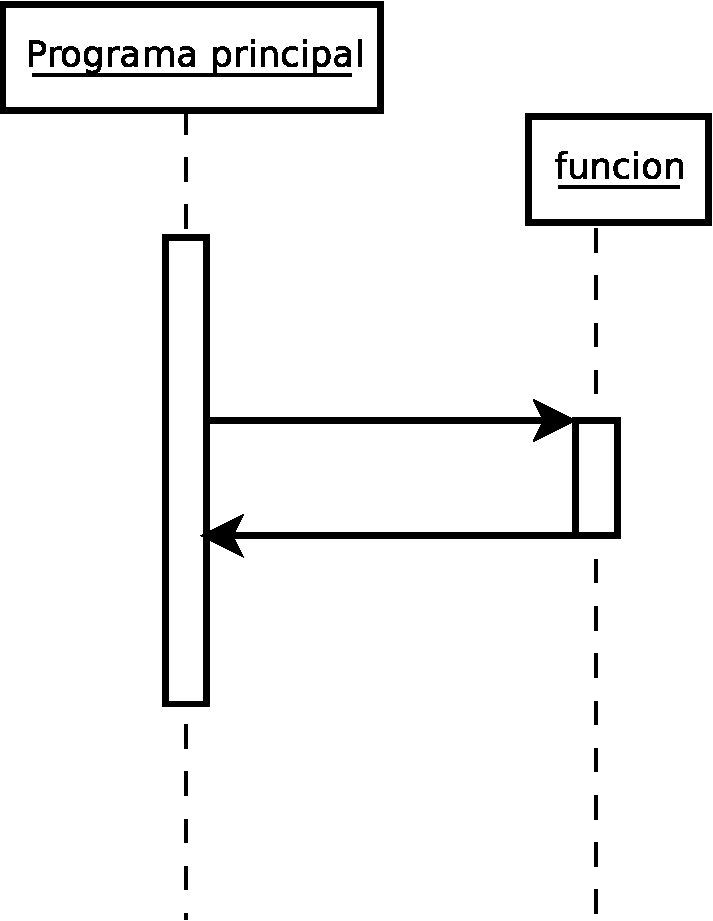
\includegraphics[%
  width=5cm,
  keepaspectratio]{figuras/Diagram1}


  \caption{\label{cap:Comportamiento-normal-de}Comportamiento normal
    de una variable llamada por una función}
\end{figure}


Si le damos a una variable el atributo de \emph{global} con la palabra
clave \texttt{global\index{global}} entonces esta variable podrá ser
vista por cualquier unidad de código sin necesidad de llamarla en su
cabecera. A estas variables no les importa si están en el programa
principal o en una función, su contexto es toda la ejecución; pueden
saltar a cualquier hilo como en el esquema de la figura
\ref{cap:Comprtamiento-de-una}:

%
\begin{figure}[h]
  \centering{}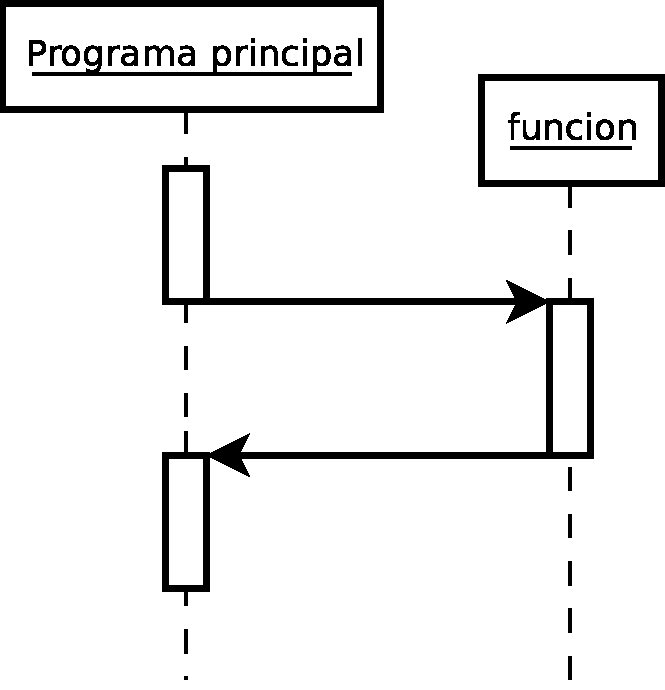
\includegraphics[%
  width=5cm,
  keepaspectratio]{figuras/Diagram2}


  \caption{\label{cap:Comprtamiento-de-una}Comportamiento de una
    variable global definida en el programa principal}
\end{figure}


Al estar definida como una variable global no sólo puede ser vista por
la función; si además la función cambia su valor también cambiará en
el programa principal. Un ejemplo de ello es el código siguiente:

\begin{verbatim}
>> global x=2
>> x
x = 2
>> function f()
global x
x=3
end
>> f()
x = 3
\end{verbatim}
Como se ve debemos tener cuidado con los nombres de las variables
globales, no es difícil estropear el código llamando una variable
global en una función sin querer%
\footnote{El uso de las variables globales es una de las pocas
  discusiones de estilo abiertas. En otros lenguajes de programación,
  sobre todo los que permiten la programación orientada a objetos, no
  es necesario utilizar este tipo de variables. Es una discusión entre
  dos escuelas.  Los que estamos más acostumbrados a una programación
  modular (Fortran) nos sentimos más cómodos controlando el hilo de
  ejecución con variables globales. En cambio, la escuela procedente
  de C++ y de Java prefieren crear métodos mucho más ricos en los que
  las funciones son en realidad métodos de un objeto que puede haber
  sido inicializado previamente.

  Creo que para un principiante el uso de variables globales es un
  buen ejercicio mental para aprender que hay distintos niveles de
  ejecución en la programación modular sin entrar en conceptos que
  muchos usan pero sólo unos pocos entienden.%
}.

Un tercer atributo es el de \texttt{persistent}\index{persistent}.
Cuando dentro de una función indicamos que una variable es
\texttt{persistent} estamos imponiendo que esta variable se guarde en
memoria para la siguiente vez que se llame la función en vez de
hacerla desaparecer, como es normal. El diagrama conceptual es el de
la figura \ref{cap:Propiedades-de-una}.

%
\begin{figure}[h]
  \centering{}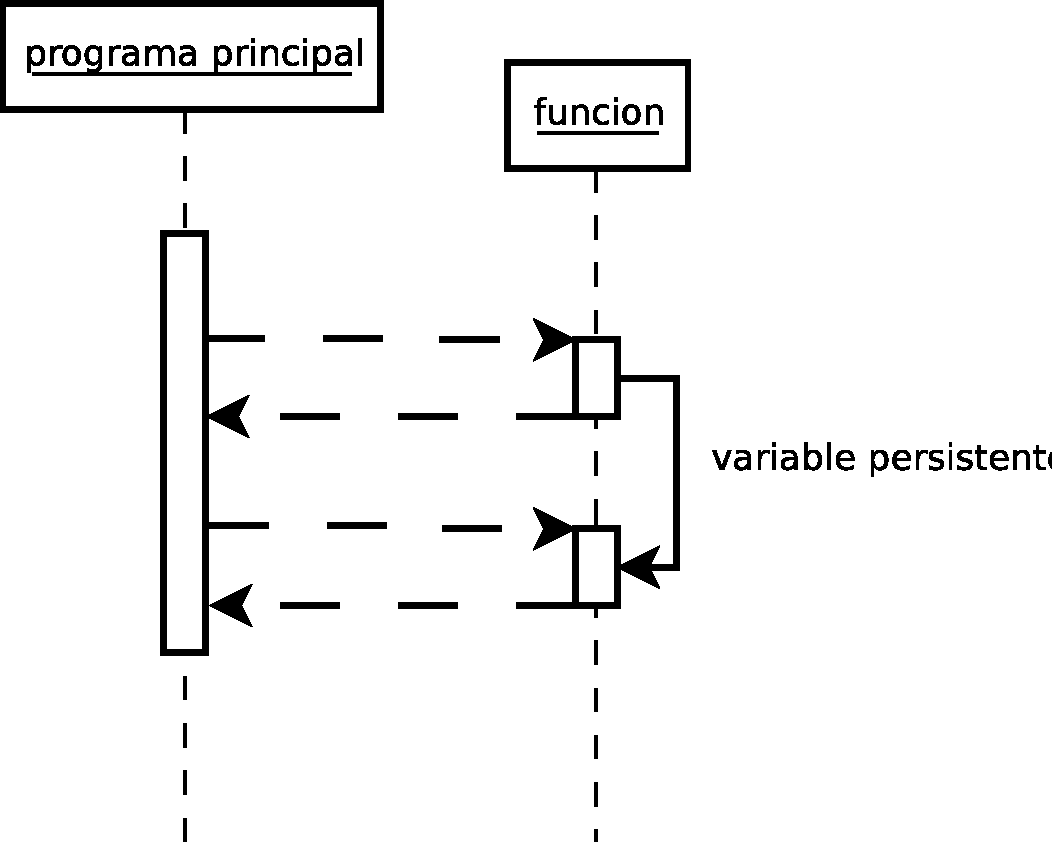
\includegraphics[%
  width=7.5cm]{figuras/Diagram3}


  \caption{\label{cap:Propiedades-de-una}Propiedades de una variable
    persistente.}
\end{figure}


No tiene ningún sentido definir una variable como \texttt{persistent}
en el programa principal porque las variables locales para el hilo
principal no se destruyen hasta que termina la ejecución.


\subsection{Funciones dedicadas a variables}

Tenemos varias funciones íntimamente relacionadas con el concepto de
variable, algunas de ellas son:

\begin{itemize}
\item \texttt{is\_global} que devuelve un $1$ en el caso que la
  variable efectivamente lo sea
\item \texttt{clear\index{clear}} que borra el contenido de una o
  varias variables, funciones o variables globales dependiendo del
  parámetro que le pasemos
\item \texttt{who\index{who}} que da una lista de las variables que en
  aquél mismo momento estén ocupadas por algún argumento. También
  acepta parámetros para variar su comportamiento.
\item \texttt{whos\index{whos}} , lo mismo que \texttt{who} pero nos
  da más información.
\end{itemize}
\begin{description}
\item [Importante:]Es necesario entender el concepto de variable local
  y global para comunicar funciones y scripts de una manera eficiente
\end{description}

\subsection{Contenedores\index{Contenedores}}

La limitación las matrices es que sólo pueden contener
elementos de un mismo tipo.  Una matriz no puede contener una cadena
de caracteres y un número a la vez.  Si sumamos mentalmente dos
matrices entenderemos facilmente por qué.

Necesitemos entonces definir un \emph{tipo\index{tipo}}
más complejo que un caracter o un escalar.  Un \emph{tipo derivado
\index{tipo derivado}}
es una extensión del concepto de argumento en el que se permite que una
variable contenga un argumento múltiple con elementos de distinta
naturaleza.  Un tipo derivado es lo que permite asignar a una variable
un número y una cadena de caracteres a la vez.

La estructura típica de los tipos derivados es la que tiene forma
de árbol.  Son llamadas \emph{estructuras de datos}.  En ellas, una
variable primitiva contiene más variables adicionales que a su vez
pueden contener más ramificaciones. Otro tipo es emular el comportamiento
de una matriz o un vector y permitir que sus elementos sean de tipos
distintos.  Obviamente esta ganancia de potencia se pierde en los
operadores.  Una matriz puede ser sumada a otra matriz, en cambio un
tipo derivado no puede ser sumado a otro tipo derivado ya que Matlab
no tiene ninguna información de qué contiene cada uno.

Esto hace que la línea divisoria entre el concepto de variable y
el de argumento se difumine.  Podemos pensar en una matriz como
un único argumento donde todos los elementos son del mismo tipo
y los tipos derivados como estructuras de variables.  Entrar en 
sutilezas teóricas no es muy conveniente, simplemente debemos
centrarnos en la gran utilidad de las estructuras de datos o las
celdas de variables ya que permiten agrupar en forma de única
variable estructuras más complejas de lo habitual.


\subsubsection{Estructuras\index{Estructuras} de datos}

Octave, al igual que la mayoría de los lenguajes de programación
modernos, nos permite agrupar variables en estructuras tipo árbol.
Podemos entonces agrupar distintos tipos de argumentos dentro de una
variable. Para probar esta posibilidad vamos a escribir un script de
prueba que se va a llamar \texttt{estructura.m}.

\begin{verbatim}
% estructura.m

% Éste es el script de prueba para las variables de tipo estructura
foo.num=1.234;   
foo.string='hola mundo';   
foo.options.option1=true;   
foo.options.option2=false;
\end{verbatim}
Lo guardamos en el directorio correspondiente y si nos vamos a la
consola y tecleamos \texttt{estructura} qué obtenemos? Pues nada en
absoluto porque le hemos pedido con los puntos y coma que no nos
sacara ninguna información por pantalla. Si queremos que nos diga qué
hay dentro de la variable \texttt{foo} debemos teclear \texttt{foo} en
la consola y nos aparecerá lo siguiente:

\begin{verbatim}
>> estructura
>> foo   
foo =   
{   
  num = 1.2340   
  options =   
  {   
    option1 = 1   
    option2 = 0   
  }   
  string = hola mundo   
}
\end{verbatim}
que es exactamente la estructura de argumentos que hemos introducido
%
\footnote{Si queremos que Octave nos saque cualquier argumento por
  pantalla podemos usar la función \texttt{disp()}\texttt{\emph{.}} En
  este caso
  al final de nuestro script podríamos añadir:\\
  \texttt{disp('nuestra estructura es')}~\\
  \texttt{disp(foo)} %
}. Vemos la manera de introducir comentarios en un script de Matlab,
con el signo \texttt{\%}. Todo lo que escribamos a partir de éste
símbolo será ignorado por el intérprete.

Además de muchas otras, la mayor utilidad de las variables de tipo
\emph{estructura} es que nos permiten acortar las cabeceras de las
funciones. Pongamos como ejemplo un programa que se configura con unos
veinte parámetros. Si una función necesita quince de ellos significa
que cada vez que llamemos a la función en nuestro código aparecerá una
cabecera con quince variables. Esto haría el código más pesado de
escribir y mucho más difícil de leer y mantener. Podemos poner todos
nuestros parámetros dentro de una variable que se llame
\texttt{parms}, de tal manera que siempre que necesitemos un
parámetro, por ejemplo \texttt{Longitud}, en cabecera simplemente
llamamos a \texttt{parms} y dentro del programa nos referimos a
\texttt{parms.Longitud}.


\subsubsection{\emph{Cell Arrays}\index{cell arrays}.}

Las celdas\index{celdas} son matrices o hiper-matrices de variables.
No debemos confundirlas con las matrices usuales que son estructuras
de argumentos del mismo tipo. Una celda puede contener matrices,
cadenas de texto y argumentos lógicos a la vez siempre que estén en
celdas separadas. A diferencia de las estructuras de datos no
tendremos que asignar un nombre a cada una de las celdas porque ya se
les asignará un grupo de índices.

Podemos construir celdas de dos modos, el primero es declarar una
variable como \texttt{cell} y darle una dimensiones. Por ejemplo
construiremos una celda de 2 por 2 cuyos elementos parecidos a los
contenidos en la estructura de datos \texttt{foo}:

\begin{verbatim}
>> foo = cell(2,2)
foo =
{
  [1,1] = []
  [2,1] = []
  [1,2] = []
  [2,2] = []
}
>> foo{1,1}=1.2340;
>> foo{1,2}=[1,2;3,4];
>> foo{2,1}='hola mundo';
>> foo{2,2}=true;
>> foo
foo =
{
  [1,1] = 1.2340
  [2,1] = hola mundo
  [1,2] =
    1  2
    3  4
  [2,2] = 1
}
\end{verbatim}
Como en el caso de las matrices convencionales podremos ampliar las
celdas con sólo llenar una que no tenga ningún argumento asignado; las
celdas {}``sobrantes'' quedan vacías:

\begin{verbatim}
>> foo{3,1}=false
foo =
{
  [1,1] = 1.2340
  [2,1] = hola mundo
  [3,1] = 0
  [1,2] =
    1  2
    3  4
  [2,2] = 1
  [3,2] = []
}
\end{verbatim}
El otro modo de iniciar una estructura de celdas es hacer lo mismo que
con una matriz pero usando llaves en vez de corchetes. Para iniciar
las celdas \texttt{foo} pero de modo abreviado:

\begin{verbatim}
>> foo={1.2340,[1,2;3,4];'hola mundo',true}
foo =
{
  [1,1] = 1.2340
  [2,1] = hola mundo
  [1,2] =
    1  2
    3  4
  [2,2] = 1
}
\end{verbatim}
\begin{description}
\item [Importante:]Las celdas pueden almacenar cualquier tipo de
  argumento, incluso funciones. Es más fácil y rápido escribirlos
  utilizando llaves.
\end{description}

\subsubsection{La necesidad de los cell arrays y los tipos derivados}
No todo en un lenguaje de programación son aplicaciones sencillas
donde escalares, vectores y matrices bastan.  Tampoco es cierto que
el dato más complejo suelen ser los argumentos que pasamos a las
funciones.  Un programa puede requerir variables que contengan tipos
de gran complejidad, normalmente obligados por el propio algoritmo.

Supongamos que intentamos una población de datos especialmente compleja,
algo usual en una base de datos.  Pongamos como ejemplo una descripción
de todos los trabajadores de una empresa.  Esto es un ejemplo, seguramente
no utilizaremos un lenguaje de programación orientado a cálculo numérico
para resolver un problema como este pero otras aplicaciones como los
algoritmos genéticos pueden requerir tipos derivados especialemnte complejos.

Sigamos con el ejemplo definiendo nuestro tipo Empleado.  Cada empleado
de la empresa proporciona los siguientes datos:

\begin{itemize}
\item Nombre completo
\item Nacionalidad
\item Documento de identidad
\begin{itemize}
\item Tipo
\item Número
\item Fecha de expedición
\item Fecha de caducidad
\end{itemize}
\item Dirección de contacto
\item Números de teléfono
\begin{itemize}
\item Número de la dirección de contacto
\item Teléfono movil de empresa
\item Teléfono movil personal
\end{itemize}
\end{itemize}

Cuando nuestros datos son muy complejos solemos pensar durante largo
tiempo el método más adecuado de almacenar todos los datos.  Crear una
variable para cada trabajador no es muy recomendable porque es probable
que tengamos que iterar sobre el total de ellos.  Tampoco parece muy
inteligente partir todos los datos en varias matrices y relacionarlas
según los índices.

La abstracción llevada a los lenguajes de programación modernos tiene
una consecuencia muy importante:  \emph{debemos ser capaces de seguir
uilizando las mismas herramientas de programación sea cual sea el dato
con el que estemos trabajando}.  Si un lenguaje se ha diseñado con el
paradigma de la abstracción como prioridad podremos seguir escalando
la complejidad de las estructuras de datos tanto como queramos sin perder
las herramientas de cálculo.  Matlab no es un prodigio en este sentido
pero se defiende bien.

El elemento que mantiene la escalabilidad en las estructuras complejas
de datos son los cell arrays.  Al seguir una estructura matricial pueden
encapsularse tantos cell arrays como queramos.  Pueden contener tanto los
tipos básicos (números y cadenas de texto) como estructuras de datos
o otras celdas.  De este modo podemos definir la estructura empleado
del siguiente modo:

\begin{verbatim}
>> Empleado1={'Paquito Palotes Parrondo';'Deaqui';
... {'DNI',646843216,12122000,12122000};
... 'C Buenaesperanza 12 1,2';
... [666251487,555698541]}
Empleado1 =

{
  [1,1] = Paquito Palotes Parrondo
  [2,1] = Deaqui
  [3,1] =

  {
    [1,1] = DNI
    [1,2] = 646843216
    [1,3] = 12122000
    [1,4] = 12122000
  }

  [4,1] = C Buenaesperanza 12 1,2
  [5,1] =

    666251487  555698541

}
\end{verbatim}
Lo novedoso es que mantenemos la escalabilidad de la estructura
indefinidamente.  Podemos sin ninguna restricción encapsular todos
los empleados en la variable Empresa como si fueran elementos de
una fila en una celda:

\begin{verbatim}
>> Empresa={Empleado1,Empleado2,Empleado3}
\end{verbatim}

\section{Sentencias\index{Sentencias}}

Como se ha dicho antes, las estructuras esenciales del lenguaje son
los contadores y los condicionales. Más comúnmente conocidas como las
sentencias \texttt{do} y las sentencias \texttt{if}. Estas estructuras
son comunes con el resto de lenguajes de programación y de scripting
existentes. La primera es un bucle contador que permite ejecutar
varias tareas idénticas secuencialmente con la variación de diversos
índices; se pueden encapsular con otros contadores y con otras
sentencias.  La segunda permite incluir variaciones en la ejecución
del código según el cumplimiento de ciertas condiciones lógicas.

Estos no son las únicas estructuras de programación, son las más
básicas.  A partir de ellas se derivan sentencias más útiles y más
específicas como veremos a continuación.

Al igual que las funciones, las sentencias tienen un principio y un
final definido iniciado por una palabra clave.  Matlab utiliza la
notación clave-cuerpo-end al igual que Fortran; C, por ejemplo
delimita estas estructuras mediante llaves y Python utiliza el
sangrado.

En este caso Matlab y Fortran presentan una diferencia esencial.
Mientras Fortran tiene un cierre para cada una las estructuras;
\texttt{do} debe cerrarse con un \texttt{end do}, Matlab cierra todas
ellas con un \texttt{end}.  El uso sistemático de \texttt{end} puede
llevar a confusiones nefastas, es por ello que Octave también soporta
el uso de \texttt{endfor}, \texttt{endif}...

\subsection{La sentencia \texttt{if\index{if}}}

Tenemos tres formas de condicional. La más simple es:

\begin{verbatim}
if (condición)
  cuerpo
endif
\end{verbatim}
Por ejemplo:
\begin{verbatim}
>> esto=1;
>> if esto
... disp('es esto');
... end
es esto
>> esto=0;
>> if esto
... disp('es esto');
... end
\end{verbatim}

Si queremos que la sentencia no se ignore, y que si la condición no se
cumple impongamos un cuerpo distinto podemos usar la estructura:

\begin{verbatim}
if (condición)   
  cuerpo 1   
else    
  cuerpo 2   
endif
\end{verbatim}
Ejemplo:
\begin{verbatim}
>> esto=1;
>> if esto
...   disp('es esto');
... else
...   disp('es lo otro');
... end
es esto
\end{verbatim}

En la que se ve perfectamente que si no se cumple la condición 1
inmediatamente se ejecuta el cuerpo2. Si tenemos más de una condición
lógica sobre una misma variable podemos usar una condicional múltiple
de la siguiente forma:

\begin{verbatim}
if (condición 1)   
  cuerpo 1   
elseif (condición 2)   
  cuerpo 2   
...   
elseif (condición n)   
  cuerpo n   
else   
  cuerpo N   
endif
\end{verbatim}

\footnote{Mucho cuidado los programadores acostumbrados a Fortran, sea
  cual sea la variante.  Si nosotros usamos \texttt{else if} en vez de
  \texttt{elseif}, Matlab va a pensar que tenemos dos sentencias
  separadas, es decir, primero un else y luego un if dentro del else.
  Esto significa que tenemos una ejecución anómala en vez de un error.
  Es uno de estos casos en los que el programa nos ejecuta, nos da un
  resultado erróneo y nosotros no vemos de ninguna manera el error de
  programación%
} Debe recalcarse que la condición debe ser sobre la misma variable
para cerrar la lógica del condicional. En el caso que tengamos
condiciones lógicas sobre más de una variable podemos encapsular los
if sin ningún problema:

\begin{verbatim}
if (condición a)   
  if (condición b)   
    cuerpo a+b   
  else   
    cuerpo a+bN   
  endif   
else   
  cuerpo aN   
endif
\end{verbatim}
Es importante que evitemos estructuras lógicas muy complejas, porque
son difíciles de entender y de depurar; aún cuando las ha escrito uno
mismo. Se verán ejemplos de estas estructuras en la sección de
ejercicios.


\subsection{La sentencia \texttt{switch}\index{switch}.}
Lo forma general del comando es:

\begin{verbatim}
switch (variable_switch)
  case (posible_valor_variable_switch)
    comandos
  case (posible_valor_variable_switch)
...
  otherwise
    comandos adicionales
endswitch
\end{verbatim}
Esta sentencia es la misma que \texttt{case} en Fortran y
\texttt{switch} en C. Un ejemplo de su uso sería:

\begin{verbatim}
>> a = 'dos'
>> switch (a)
case ('uno')
disp('has escogido el numero 1')
case ('dos')
disp('has escogido el numero 2')
otherwise
disp('no se que numero has escogido')
endswitch
has escogido el numero 2
\end{verbatim}

\subsection{La sentencia \texttt{for\index{for}}}

Así es como se denomina el contador o sentencia \texttt{do} en Matlab.
Su estructura es:

  \begin{verbatim}
for [variable contador]=[secuencia del contador]
  cuerpo [dependiente o no de la variable contador]
endfor 
\end{verbatim}
Es decir, para una determinada variable, que avanza de 1 en 1 desde el
límite inferior hasta el límite superior ejecutamos el cuerpo.  El
cuerpo puede depender o no de la variable contador, ésta puede ser un
contador a parte, que simplemente nos imponga que una determinada
sentencia se ejecute un número fijo de veces. La mayoría de las veces
nuestro cuerpo dependerá de la variable que usemos como contador, es
decir, será un índice de nuestro cuerpo.

Notemos que lo que utilizamos para contar una secuencia, como en el
caso de las submatrices. Lo que hará el índice contador será tomar
sucesivamente todos los valores que tengamos en la secuencia. Por
ejemplo, si pedimos que una variable haga un bucle de ese tipo:

\begin{verbatim}
for i=1:2:10
\end{verbatim}
dentro del bucle la variable \texttt{i} tomará los valores que salen
por pantalla en el caso que llamemos la secuencia:

\begin{verbatim}
>> 1:2:10
ans = 1   3   5   7   9
\end{verbatim}

Por ejemplo:
\begin{verbatim}
>> for i=5:5:25
... disp(i),disp('es multiple de 5')
... end
5
es multiple de 5
10
es multiple de 5
15
es multiple de 5
20
es multiple de 5
25
es multiple de 5
\end{verbatim}


Los bucles con contador también se pueden encapsular, y éste
encapsulado es esencial cuando trabajemos con matrices de rango
mayor que 1. Por ejemplo, si queremos asignar una operación compleja a
una matriz de rango 3 debemos encapsular 3 contadores:

\begin{verbatim}
for i=1:IMAX   
  for j=1:JMAX   
    for k=1:KMAX   
      cuerpo   
    endfor   
  endfor   
endfor
\end{verbatim}


\subsection{La sentencia \texttt{while\index{while}}}

En vez de controlar el bucle mediante un contador es muy útil
controlarlo mediante una condición lógica. Para eso podemos usar una
estructura \texttt{while}.

\begin{verbatim}
while (condición)   
  cuerpo   
endwhile
\end{verbatim}

Ejemplo:
\begin{verbatim}
>> a=0;
>> while a<5
... disp(a)
... a=a+1;
... end
0
1
2
3
4
\end{verbatim}

Sólo debemos tener en cuenta cuando programamos que el uso de un while
es mucho más crítico que el uso de un for. Esto es porque la condición
lógica que controla el bucle debe aplicarse sobre una variable interna
en el bucle. Entonces es probable que si programamos mal, la variable
que usamos como control nunca llegue a cumplir la condición que nos
para la ejecución. En Matlab o Octave no suele ser un gran problema,
puesto que el sistema puede reaccionar y cortar el proceso de otro
modo, pero en otros lenguajes puede tener consecuencias bastante
desagradables.  También debemos tener en cuenta que los bucles
controlados por una condición lógica no permiten la paralelización en
el caso que tengamos una versión para varios procesadores de Matlab o
Octave.


\subsection{La sentencia \texttt{do-until\index{do-until}}}

Esta sentencia es equivalente a \texttt{while} con la condición lógica
complementaria.


\subsection{Las sentencias \texttt{break\index{break}} y
  \texttt{continue\index{continue}}}

Tanto para el \texttt{for} como para los otros tipos de bucles tenemos
variables de control de la ejecución que pueden ser de utilidad. La
sentencia \texttt{break} dentro de un bucle nos quita el hilo%
\footnote{Se llama hilo precisamente a la línea de ejecución. Nos la
  podemos imaginar como la línea de código que siguen los procesos.
  Este concepto va ligado íntimamente a la gestión de procesos y
  tiende a complicarse en lenguajes como C o Fortran.%
} del bucle para seguir ejecutando el programa o un bucle externo.  Un
ejemplo sería:

\begin{verbatim}
num=103;   
div=2;   
while (div*div <= num)   
  if (rem (num, div) == 0)   
    break;   
  endif   
  div++;   
endwhile   
if (rem (num, div) == 0)   
  printf ('El divisor menor de %d es %d \n', num, div);   
else   
  printf ('%d es primo \n', num);   
endif
\end{verbatim}
En cambio la sentencia \texttt{continue}, en vez de sacarnos del
bucle, hace que saltemos uno de los pasos del mismo para ir al
siguiente estado del contador.


\subsection{La sentencia \texttt{try\index{try}}}

Los bloques de estructura \texttt{try} son de la forma:

\begin{verbatim}
try
  cuerpo
catch 
  alternativa
end
\end{verbatim}

Por ejemplo:
\begin{verbatim}
>> a=rand(5,5);b=rand(4,4);
>> try
... a*b
... catch
... disp('Dimensiones incompatibles')
... end
Dimensiones incompatibles
\end{verbatim}

Esta estructura es muy parecida a \texttt{if-else} pero con la
particularidad que la condición lógica es si se produce o no un error.
Se usará cuando no sepamos si algo puede ejecutarse bien o no y no
queramos que el error afecte al resto de la ejecución del programa.
Primero intentará ejecutar la sentencia que hayamos puesto en
\texttt{cuerpo} y si devuelve un error ejecutará \texttt{alternativa}
ignorando el error producido por la primera sentencia.


\section{Funciones (II)}

Tratar la función en Matlab sólo desde el punto de vista de un archivo
auxiliar es un tremendo error. La escritura y manipulación de
funciones es la mayor potencia (probablemente la única) del lenguaje.
Este planteamiento choca con la formulación básica de la función y se
acerca más a los lenguajes orientados a objetos donde podemos asignar
un método a una variable, algo impensable en Fortran. Siendo poco
rigurosos podemos decir que si C++ es un lenguaje orientado a objetos
Matlab es orientado a funciones.


\subsection{Funciones matemáticas básicas}

Matlab cuenta con una enorme biblioteca de funciones matemáticas.  Su
utilidad depende directamente del conocimiento que tengamos de ellas.
Mientras intuitivamente ya hemos usado las funciones trigonométricas
\texttt{sin} y \texttt{cos}, muchas de las presentes en la colección
ni nos sonarán. Cumple el objetivo principal de ahorrarnos tener que
escribir cualquier función mínimamente conocida. El nombre que reciben
estas funciones suele ser bastante descriptivo; la función $\Gamma$ se
llamará \texttt{gamma} y las funciones de Airy se llamarán
\texttt{airy}.

Estas funciones no son archivos \texttt{.m}, se escriben en un
lenguaje compilado como C++ o Fortran para que su velocidad sea mayor.
No debemos tener miedo a usarlas tanto como sea posible.


\subsection{La Ayuda\index{Ayuda}(II)}

Ya hemos hablado del comando \texttt{help\index{help}} y cómo debe
utilizarse. Nosotros también podemos dotar nuestras funciones de una
ayuda parecida de una manera muy fácil. Todas las líneas
\textbf{comentadas} entre la sentencia \texttt{function} y la primera
sentencia ejecutable nos saldrán por pantalla si llamamos a la función
mediante el comando \texttt{help}. Por ejemplo:

\begin{verbatim}
function out=derivada_numerica(in)   
%   
% función derivada_numerica Calcula las diferencias centradas de
% primer orden de un vector entrada: in (vector) salida : out (vector)
%
   
  ...   
end 
\end{verbatim}
Cuando hagamos \texttt{help derivada\_numerica} obtendremos por
pantalla:

\begin{verbatim}
función derivada_numerica   
 Calcula las diferencias centradas de primer orden de un vector   
   entrada: in  (vector)   
   salida : out (vector)
\end{verbatim}

Disponemos también de dos funciones para manejar los errores de
ejecución, \texttt{usage} y \texttt{error}. En la sección
\ref{sub:Argumentos-de-entrada} tenemos un ejemplo de cómo se usan.
Son de gran utilidad sobre todo cuando hagamos debugging de un
programa grande. Si se produce un error en la lectura de los
argumentos o en el cálculo interno se imprime en pantalla toda la
cadena de errores que han provocado el fallo, estos mensajes son a
menudo demasiado crípticos. Si intuimos que la ejecución puede fallar
en algún sitio debemos preverlo, es una buena táctica pensar el hilo
de ejecución tanto si funciona correctamente como si no.

%
\footnote{En Octave también podemos escribir la ayuda en formato
  \emph{texinfo} para incluir caracteres matemáticos y fracciones pero
  es un tema muy avanzado.%
}


\subsection{Argumentos de entrada y
  salida.\label{sub:Argumentos-de-entrada}}

En el apartado anterior dedicado a funciones (\ref{sub:Funciones(I)})
hemos sido intencionadamente rigurosos con la sintaxis. Si una función
retorna sólo una variable pueden omitirse los corchetes:

\begin{verbatim}
function salida = entrada (arg)
  salida = ...
end
\end{verbatim}
La función \texttt{nargin\index{nargin}} retorna el número de
argumentos de entrada necesarios en una función, si lo aplicamos a la
función \texttt{entrada} que acabamos de definir\footnote{En breve
  aprenderemos que la mejor manera de llamar este tipo de funciones es
  mediante un Function handle}:

\begin{verbatim}
>> nargin('entrada')
ans = 1
\end{verbatim}
Mientras que dentro de la función es una constante cuyo valor es el
número de argumentos de entrada:

\begin{verbatim}
function retval = avg (v)
% retval = avg(v) v :: vector
%
% Calcula la media de los elementos de un vector
  retval = 0;
  if (nargin != 1)
    usage ('avg (vector)');
  endif
  if (isvector(v))
    retval = sum(v) / length(v);
  else
    error ('avg: expecting vector argument');
  endif
end
\end{verbatim}
Este ejemplo además nos sirve para ver el control de errores de una
función. Las palabras clave \texttt{usage\index{usage}} y
\texttt{error\index{error}} son los mensajes que saldrán por pantalla
si se comete un mal uso o existe un error de ejecución
respectivamente. Para que entendamos más en profundidad se propone
esta sesión de consola:

\begin{verbatim}
>> help avg
avg is the user-defined function from the file
/home/guillem/CursoScripting/ejercicios/avg.m   
retval = avg(v)
v :: vector
Calcula la media de los elementos de un vector   
>> v=[1,2,3,4];
>> avg(v)
ans = 2.5000
>> u=[4,3,2,1];
>> avg(u,v)
usage: avg (vector)
error: evaluating if command near line 8, column 3
error: called from `avg' in file `/home/guillem/C...
>> w=[1,2;3,4];
>> avg(w)
error: avg: expecting vector argument
error: evaluating if command near line 11, column 3
error: called from `avg' in file `/home/guillem/C...
>>
\end{verbatim}
Los corchetes son necesarios sólo cuando queramos retornar más de una
variable:
\begin{verbatim}
function [salida1,salida2] = entrada (args)
  salida1 = ...
  salida2 = ...
end
\end{verbatim}
En el caso que dejemos una variable vacía no vamos a obtener un error
sino un aviso:

\begin{verbatim}
>> function [x,y,z] = f()
x=1;
y=2;
end
>> [a,b,c]=f()
warning: in f near line 7, column 8:
warning: f: some elements in list of return values are undefined
a = 1
b = 2
c = []
>>                 
\end{verbatim}
Si queremos saber cuantas variables de salida tiene una función
debemos usar \texttt{nargout}\index{nargout}. Una variable de control
muy interesante es la palabra clave \texttt{return}\index{return},
Cuando el hilo de ejecución de una función pasa por la palabra
\texttt{return} inmediatamente retorna la ejecución a la consola o al
programa principal:

\begin{verbatim}
function out = any_zero(v)
% out = any_zero (v) v :: vector
%
% devuelve un mensaje si algun elemento de v es 0
out = 0;
for i = 1:length(v)
  if (v (i) == 0)
    out = 1;
    return
  endif
endfor
printf ('No se ha encontrado ningun cero \n')   
>> u=[1,2,3,0];
>> v=[1,2,3,4];
>> any_zero(u)
ans = 1
>> any_zero(v)
No se ha encontrado ningun cero
ans = 0
\end{verbatim}

\subsection{\texttt{inline\index{inline}}}

Si Matlab no puede definir funciones completas dentro de un script
significa que para escribir cualquier expresión matemática no básica
debemos crear un archivo. Esto no es del todo cierto por la sentencia
\texttt{inline}. Lo que hace es interpretar una cadena de texto en la
que escribimos una función y la conecta a una variable, como si de un
puntero a una función se tratara. Su uso es muy sencillo, pero
requiere cierta práctica.

Si queremos introducir una función escribiremos:

\begin{verbatim}
>> foo=inline('sin(x)*cos(x)','x');
\end{verbatim}
En la que obviamente introducimos los elementos como cadenas de texto.
Para evaluar la función lo haremos del modo usual:

\begin{verbatim}
>> c=foo(6)
\end{verbatim}
que nos pondrá en la variable \texttt{c} el valor de la función en 6,
-0.26829.

En el caso que nuestra función tenga más de una variable de entrada
podemos explicitarlas como:

\begin{verbatim}
>> foo2=inline('sin(x)*cos(y)','x','y');
\end{verbatim}
Entonces los parámetros de entrada para la evaluación van a ser dos y
van a mantener el orden asignado en la sentencia \texttt{inline}.  De
hecho, este intrinsic funciona perfectamente con sólo la función como
argumento, pero es casi un imperativo para saber cómo se introducen
las variables en la evaluación.

También podemos utilizar la sentencia \texttt{inline} cuando se nos
pida evaluar una función. Vimos un ejemplo de ello en el primer
capítulo cuando se introdujo el lenguaje:

\begin{verbatim}
>> quad(inline('besselj(2.5,x)'),0,4.5)
ans = 1.1178
\end{verbatim}

Para integrar necesitamos una función de una sola variable de modo que
hemos creado una nueva función con la sentencia \texttt{inline} para
modificar la función \texttt{besselj}. La nueva función (sin nombre)
acepta sólo un argumento. Esta práctica es muy frecuente y útil,
pensemos que por cada vez que utilicemos un \texttt{inline} nos
ahorramos un archivo.


\subsection{Function handles\index{function handles}}

Hemos enfatizado en la necesidad de diferenciar los conceptos de
variable y de argumento. Ahora introduciremos un concepto aún más
complejo, el de la manipulación de funciones. En Matlab la función no
es un elemento inerte como en Fortran, se parece bastante más a las
funciones de C. Un ejemplo de esta diferencia es que en C podemos
crear matrices cuyos elementos sean funciones gracias al uso de
punteros.

Fuera de estas consideraciones teóricas diremos que Matlab tiene una
herramienta para asignar funciones (aunque sería más correcto
llamarlos métodos) a variables. Esta herramienta se llama Function
handle por comparación con una herramienta real, sería conveniente
llamarla {}``asa'' o {}``mango''. Pensemos en un martillo; la
herramienta en sí es sólo la cabeza y lo que nos ayuda a manejarlo es
el mango cuya función, aunque secundaria, es imprescindible. Lo mismo
sucede con las asas de una paellera. Las funciones en un archivo son
como paelleras sin asas, cumplen su función pero no las podemos
manejar. Si utilizamos los Function handles para asignar una función a
una variable podemos utilizar la función sin hacerlo directamente al
igual que operamos los argumentos mediante variables.

Un Function handle se denota con la letra \texttt{@}. Por ejemplo, si
queremos asignar a la variable \texttt{varsin} la función $\sin$ lo
haremos del siguiente modo:

\begin{verbatim}
>> varsin = @sin
\end{verbatim}
A partir de ahora la variable sirve de interfaz a la función. Da igual
que la función sea parte de la biblioteca estándar o que la acabemos
de escribir nosotros mismos. Por si hay alguna duda de que
\texttt{varsin} es ahora la función seno:

\begin{verbatim}
>> varsin(pi/2)

ans = 1
\end{verbatim}
Un uso muy interesante de los Function handles es la creación de
estructuras de datos con funciones. Como ejemplo crearemos unas celdas
donde los elementos sean las funciones trigonométricas básicas:

\begin{verbatim}
>> trifun={@sin,@cos,@tan}
trifun =
{
  [1,1] =
sin
  [1,2] =
cos
  [1,3] =
tan
}
>> trifun{3}(pi/4)
ans = 1.0000
\end{verbatim}
Esto hace que tengan un papel protagonista en las cabeceras de las
funciones. Cuando una función necesita a otra como argumento podemos
asignarla también por nombre o por una sentencia \texttt{inline} pero
lo recomendable es utilizar un Function handle. Por ejemplo, para
hacer la siguiente integral mediante la función \texttt{quad}:

$$I=\int_{0}^{\pi}\sin(x)\ dx$$


\begin{verbatim}
>> I=quad('sin',0,pi)
I = 2
>> I=quad(inline('sin(x)'),0,pi)
I = 2
>> I=quad(@sin,0,pi) # Forma recomendada
I = 2
\end{verbatim}
La tercera es equivalente a pasar antes el Function handle con la
función seno a una variable:

  \begin{verbatim}
>> fhandle=@sin
fhandle =
sin
>> I=quad(fhandle,0,pi)
I = 2
\end{verbatim}
Y así con todas las rutinas que requieran una función como argumento.


\subsubsection{Funciones anónimas\index{funciones anónimas}}

La sentencia \texttt{inline} se considera obsoleta (aunque no
oficialmente).  El recurso que la ha apartado es utilizar un Function
handle para declarar una función con la siguiente sintaxis:

\begin{verbatim}
@(argumentos) sentencia_ejecutable
\end{verbatim}
Por ejemplo, la función \texttt{foo2} que en la sección anterior se ha
declarado mediante un \texttt{inline} se escribiría como sigue:

\begin{verbatim}
>> foo2 = @(x,y) sin(x)*cos(y)
\end{verbatim}
Con la llamada usual:

\begin{verbatim}
>> foo2(6,2)
ans = 0.11628
\end{verbatim}
Obviamente también podemos utilizarlo en la cabecera de las funciones:

\begin{verbatim}
>> quad(@(x) besselj(2.5,x),0,4.5)
ans = 1.1178
\end{verbatim}
Alguien puede pensar que el nombre de {}``función anónima'' está mal
porque si la asignamos a una variable pasará a tener el nombre de la
variable. Esta idea, aunque razonable, es completamente errónea.  Una
y otra vez hemos enfatizado que una variable no es un argumento ni una
función, es algo completamente distinto. La función es anónima porque
no tiene ningún nombre fijo, seguirá siendo la misma función
independientemente del nombre de la variable.


\subsubsection{Funciones como argumentos de funciones.}

Si gracias a los Function handles podemos asignar funciones a
variables esto nos servirá para pasar funciones como argumentos. Una
de las prácticas más beneficiosas en programación es la de la
\emph{introspección}\index{introspección}.  Es la capacidad de un
algoritmo de no depender de los argumentos que utilicemos. La
introspección más común es la aplicada a los números y las matrices;
es lo que sucede cuando escribimos cualquier fórmula matemática o
función en Matlab, pero aplicar la introspección a las funciones no es
tan sencillo. Es muy fácil integrar una función cuando la conocemos,
lo que no es integrar una función cualquiera. Debemos encontrar
automáticamente los puntos singulares para concentrar los puntos en
ellos, controlar automáticamente la precisión y pasar un argumento a
la función. La introspección es intentar hacer un algoritmo lo más
genérico posible y para ello necesitamos llamar funciones como
argumentos como sucede con las rutinas de integración.

Si lo pensamos un poco nos daremos cuenta que no es nada fácil llamar
a una función cuyo nombre no conocemos y sin saber en qué directorio
se encuentra. La solución a este problema son los Function handles,
por eso se recomienda encarecidamente su uso. Supongamos que queremos
una rutina que calcule el valor de cualquier función en el punto $x=1$
siendo $x$ su único argumento:

\begin{verbatim}
function [out]=fhtest(arg)
%
% function OUT=fhtest(@arg)
%
% Calcula el valor de la funcion @arg en 1 @arg debe ser un Function
% Handle
%
out=arg(1);
\end{verbatim}
\emph{Es muy importante crear una cabecera de ayuda cuando los
  argumentos de una función no son escalares comunes. Si no será
  imposible saber que el argumento de} \texttt{\emph{fhtest}} \emph{es
  un Function handle.  Lo correcto sería crear también un mensaje de
  error en el caso que el argumento no fuera del tipo adecuado. Cuando
  una función no devuelve ningún resultado lo primero que haremos será
  utilizar la ayuda:}

\begin{verbatim}
>> help fhtest
fhtest is the user-defined function from the file
/home/guillem/sync/CursoScripting/ejercicios/fhtest.m
 function OUT=fhtest(@arg)
 Calcula el valor de la funcion _arg_ en 1
  _arg_ debe ser un Function Handle
\end{verbatim}
será un alivio comprobar que existe.  Para utilizar la función podemos
llamarla directamente con un Function handle:

\begin{verbatim}
>> fhtest(@sin)
ans = 0.84147
\end{verbatim}
o como siempre mediante una variable que lo contenga:

\begin{verbatim}
>> fhsin=@sin
fhsin =
sin
>> fhtest(fhsin)
ans = 0.84147
\end{verbatim}
Esta estructura permite hacer


\subsubsection{Acceso a las variables desde las funciones anónimas.}

Otra pequeña diferencia entre Matlab y Octave es cómo las funciones
anónimas entienden las variables dadas en la cabecera. En Octave, una
función anónima es estrictamente una función a parte. Las variables
internas no tienen ninguna relación con las variables del resto del
entorno de ejecución. Por ejemplo, si queremos definir la siguiente
función de dos variables:

$$func=e^{-(x^{2}+y^{2})}$$

a partir de una función anónima debemos hacerlo como

\begin{verbatim}
>> func=@(x,y) exp(-(x. ^2+y. ^2)) 
func =
@(x, y) exp (-(x . ^ 2 + y . ^ 2)) 
\end{verbatim}
Y llamamos la nueva función del modo usual:

\begin{verbatim}
>> func(sqrt(log(5)),sqrt(log(5)))
ans = 0.040000 
\end{verbatim}
Todas estas variables son locales para la función. Todas las variables
de la función deben estar presentes en el interface. Se nos puede
ocurrir reducir el número de variables de una función definiendo
algunas de ellas externamente:

\begin{verbatim}
>> a=2;
>> func=@(x) exp(-(x. ^2+a. ^2)) 
func =
@(x) exp (-(x . ^ 2 + a . ^ 2))
\end{verbatim}
De este modo estamos pidiendo que la función tome una variable que en
realidad es externa como propia. En Octave esto da un error en el
momento de la llamada:

\begin{verbatim}
>> func(2)
error: `a' undefined near line 9 column 22
error: evaluating binary operator `. ^' near line 9, column 23
error: evaluating binary operator `+' near line 9, column 21
error: evaluating prefix operator `-' near line 9, column 15
error: evaluating argument list element number 1
error: called from `?unknown?'
\end{verbatim}

Pero si hacemos exactamente lo mismo en Matlab...

\begin{verbatim}
>> a=2;
>> func=@(x) exp(-(x. ^2+a. ^2))
func =
    @(x) exp(-(x. ^2+a. ^2))
>> func(2)
ans =
   3.3546e-04
>>
\end{verbatim}
El programa el intérprete no nos devuelve ningún error. Esto es debido
a que mientras Octave prefiere la definición de variables globales

como apuesta por la seguridad, Matlab es más laxo con el acceso a las
variables en el caso de los function handles. De hecho, este es el
modo recomendado por los desarrolladores de Matlab para acortar
algunas cabeceras mediante variables externas o para pasar parámetros
a funciones dentro de funciones.


\subsection{Funciones recursivas\index{recursivas}}

Matlab soporta funciones que durante su ejecución se llaman a ellas
mismas porque las llamadas a las funciones se hacen por valor y no por
variable. Es muy difícil encontrar un ejemplo donde la manera más
efectiva de resolver un problema sea acudir a la recursión. Es una
técnica peligrosa además de ser muy agresiva con la memoria y debemos
evitarla. Un ejemplo de función recursiva sería esta manera tan poco
eficiente de calcular un factorial\index{factorial}%
\footnote{Existen varias maneras de calcular un factorial. Las dos más
  eficientes probablemente sean \texttt{prod(1:n)} y
  \texttt{gamma(n+1)}%
}.

\begin{verbatim}
function out = fact ()
  if (n > 0)
    out = n* fact (n-1);
  else
    out = 1;
  endif
\end{verbatim}

\subsection{Encapsulado de funciones}

El encapsulado de funciones o \emph{nested functions} tiene dos
utilidades principales:

\begin{enumerate}
\item Encapsular partes del cálculo en una función principal dentro de
  una función secundaria
\item Posibilitar que argumentos de salida sean funciones mediante
  function handles.
\end{enumerate}
El primer uso es trivial. Podemos definir \emph{subfunciones} siempre
que no tengan ninguna repercusión en la cabecera. No es más que
agrupar una tarea repetitiva para no tener que escribirla varias
veces.

El segundo uso es una de las sutilezas proporcionadas por los function
handles. Como podemos definir subfunciones siempre que no influyan en
la cabecera nada nos impide asignarlas a un function handle que se
pasará en la salida como argumento. Es exactamente el mismo concepto
que el de utilizar funciones como argumentos de funciones pero a la
inversa.

Por ejemplo, supongamos que estamos diseñando un filtro para una
señal, un filtro pasa-bajos según una determinada frecuencia $\omega$.
Lo más sencillo sería hacer una función pasa-bajos que recibiera tres
argumentos, el espectro en frecuencias, la longitud del espectro y la
frecuencia de corte. Una solución mucho más elegante puede ser definir
una función de construcción que devuelve un function handle con un
filtro que utilizamos como otra función por separado. De este modo
conseguiríamos reducir toda una colección de filtros a una única
función generadora. Esta práctica se llama introspección y es junto
con la abstracción las dos palabras claves de la programación moderna.
La capacidad de Matlab de convertir funciones en argumentos simples es
la mayor potencia del lenguaje y a la vez el concepto más complejo.
Dominar bien la abstracción a nivel de métodos es dominar Matlab.


\subsection{Sobrecarga de funciones.(Octave)}

\emph{Este es un tema bastante avanzado sólo interesante para la
  programación de algoritmos muy complejos. Octave proporciona varias
  subrutinas para la gestión de la sobrecarga de funciones que no he
  sido capaz de encontrar en Matlab. La única herramienta equivalente
  que Matlab posee son las funciones} \texttt{\emph{inferiorto}}
\emph{y} \texttt{\emph{superiorto}} \emph{que controlan la preferencia
  de búsqueda de funciones en el árbol de directorios. Dudo que nadie
  de los que lea este libro tenga necesidad de utilizar la sobrecarga
  jamás pero puede ser útil cuando se construyen prototipos de
  programas en Fortran 95. También son útiles en el caso que estemos
  programando interfaces a otros programas en C++ donde el tipo de
  argumento es importante. Imaginemos que acabamos de implementar una
  función en C que se comporta de un modo distinto si el argumento es
  un número real o un complejo. En Octave no tendríamos absolutamente
  ningún problema porque trata ambos tipos del mismo modo pero C es
  otra historia. Si nuestro código fuera sólo C tendríamos que
  programarnos un interfaz que seleccionara la función según la
  entrada; sobrecargar la función desde Octave es una solución mucho
  más elegante.}

Los dos conceptos más importantes de la programación moderna son la
abstracción y la introspección. La primera nos dice que debemos
abstraernos de lo que estamos calculando, debemos centrarnos en el
concepto y no ver un \texttt{2+3} sino un a\texttt{+b}. La
introspección va un poco más lejos; la idea es no sólo abstraernos del
contenido de cada variable sino abstraerse también del método
utilizado. La abstracción la dan las fórmulas matemáticas y la
introspección los interfaces.

Dentro de los métodos de introspección uno de los más utilizados es la
sobrecarga de funciones. Es un tema bastante avanzado pero puede
aportar grandes beneficios en códigos muy complejos. Sobrecargar una
función es asignar más de un método a un nombre y aportarle un método
adicional para que según el tipo de argumento se use un método o otro.

\begin{description}
\item [dispatch\index{dispatch}]Función que se encarga de gestionar la
  sobrecarga de métodos en un nombre. Para saber qué método llamar
  utiliza una pequeña referencia que asigna cada tipo a una función.
  También nos permite administrar los interfaces para añadir y
  eliminar funciones a la sobrecarga.
\end{description}
Por ejemplo, si utilizamos la función \texttt{dispatch} con la función
exponencial vemos que en realidad es un método sobrecargado
dependiente del tipo:

\begin{verbatim}
octave:1> dispatch('exp')
Overloaded function exp
exp(fixed complex,...)->fexp(fixed complex,...)
exp(fixed complex matrix,...)->fexp(fixed complex matrix,...)
exp(fixed matrix,...)->fexp(fixed matrix,...)
exp(fixed scalar,...)->fexp(fixed scalar,...)
exp(galois,...)->gexp(galois,...)
\end{verbatim}
\texttt{fexp} y \texttt{gexp} son funciones llamadas \emph{builtin
  functions} que son funciones de un nivel mucho más bajo que no
serían útiles por sí solas.

\begin{description}
\item [builtin\index{builtin}]Permite acceder a una función básica
  ignorando el \emph{dispatch} que tenga sobre ellas.
\end{description}
Todo lo que es potente es complejo y estos conceptos son ambas cosas.
Es importante que sólo usemos estas herramientas cuando las dominemos.


\subsection{Herramientas útiles para la manipulación de funciones.}

\begin{description}
\item [addpath\index{addpath}]Añade uno o varios directorios a la
  lista de la base de datos de funciones.
\item [edit\index{edit}]Llama al editor descrito en la variable
  \texttt{EDIT} para editar la función pasada como argumento
\item [type\index{type}]Muestra información rápida sobre la variable o
  el nombre de la función. Si el argumento es una función o una
  subrutina dentro de un archivo \texttt{.m} muestra el contenido del
  archivo.
\end{description}

\section{Entrada/Salida}

Supongamos que hemos hecho un script para calcular la solución a un
problema de control y necesitamos que en el arranque el usuario nos
introduzca los datos de entrada, o pongámonos en la situación de estar
utilizando un código de mecánica de fluidos computacional que nos
escupe enormes matrices de datos en crudo.

Cualquier interacción de nuestro programa con el exterior necesitará
funciones de comunicación, ya sea un pequeño diálogo en la consola o
la lectura de matrices de gran tamaño. El primer caso es bastante
sencillo pero el segundo requiere conocimientos básicos de
almacenamiento de datos que aprenderemos en breve.


\subsection{E/S básica por pantalla.}

\begin{description}
\item [disp]Es la función de salida más sencilla. Imprime en pantalla
  el argumento con el que se llama ya sea una cadena de texto o el
  contenido de una variable.
\item [format]Controla el formato numérico de salida por defecto. Es
  importante que entendamos que sólo cambia la impresión en pantalla o
  en un archivo, no estamos cambiando la precisión numérica real.
  \texttt{format} se
  llama con un argumento que determina el tipo de salida:\\
  \\
  \begin{minipage}[c]{0.8\columnwidth}%
    \texttt{short\index{short}} Formato con 5 cifras significativas en
    contenedores de 10 caracteres. Si el punto decimal se sale de las
    cifras significativas en algún caso todos los números pasaran a
    escribirse según la notación científica.

    \texttt{long\index{long}} Formato con 15 cifras significativas en
    contenedores de 20 caracteres. Si el punto decimal se sale de las
    cifras significativas en algún caso todos los números pasaran a
    escribirse según la notación científica\end{minipage}%
  \\
  \\
  \\
  \begin{minipage}[c]{0.8\columnwidth}%
{\texttt{short e}} 

{\texttt{long e}} El mismo formato que \texttt{short} y \texttt{long}
pero usando siempre la notación científica y denotando el exponencial
con una \texttt{e}.\end{minipage}%
\\
\\
\\
\begin{minipage}[c]{0.8\columnwidth}% 
{\texttt{short E}} 

{\texttt{long E}} El mismo formato que \texttt{short} y \texttt{long}
pero usando siempre la notación científica y denotando el exponencial
con una \texttt{E}.\end{minipage}%
\\
\\
\\
\begin{minipage}[c]{0.8\columnwidth}%
{\texttt{short g}} 

{\texttt{long g}} Escoge entre el formato usual o la notación científica
según lo requiera cada número. En el caso de la notación científica
la exponencial se denota con una \texttt{e}.\end{minipage}%
\\
\\
\\
\begin{minipage}[c]{0.8\columnwidth}%
{\texttt{short G}} 

{\texttt{long G}} Escoge entre el formato usual o la notación
científica según lo requiera cada número. En el caso de la notación
científica la exponencial se denota con una \texttt{E}.\end{minipage}%
\\
\\
\\
\begin{minipage}[c]{0.8\columnwidth}%
\texttt{free\index{free}} 

\texttt{none\index{none}} Formato libre igual al formato libre de
Fortran.\end{minipage}%

\item [input\index{input}]Es el equivalente a \texttt{disp} pero para
  la introducción de valores por teclado. Imprime por pantalla lo
  pedido en el argumento y espera a la escritura de un valor por
  teclado.
\item [{menu (tit,op1,...)}]Imprime en pantalla el menú\index{menú}
  con un título y las opciones del argumento, cada una de las opciones
  se presenta con un número y espera que se escoja uno de ellos por
  teclado.  El valor retornado es el número de la opción escogida.
  Cuando se está utilizando la interfaz gráfica de Matlab aparece una
  ventana y que muestra un botón por cada opción Por ejemplo:
\end{description}
  \begin{verbatim}
>> choice=menu('Esto es un menu','uno','dos','tres')
Esto es un menu
  [ 1] uno
  [ 2] dos
  [ 3] tres
pick a number, any number: 3
choice = 3
\end{verbatim}

\subsection{E/S básica con archivos}

Las palabras clave para guardar variables y sesiones son compatibles
pero no idénticas. Esto es porque mientras Matlab tiene sus propios
formatos de lectura y escritura Octave ha optado por formatos
abiertos%
\footnote{Uno de los apéndices trata de la importancia del uso de los
  formatos abiertos%
}.

Matlab puede leer y escribir archivos en formato binario; esto
necesita una pequeña explicación. Hay dos maneras principales de
almacenar números en memoria, en formato texto y en formato binario.
En el primer caso se escriben en un fichero que un humano puede leer,
normalmente codificado en ASCII de 8 bits. El programa se encarga de
alinear las columnas y situar la coma para poder leerlo cuando sea
oportuno. El precio de mantener cada número como algo leíble tiene un
coste en memoria mucho mayor, esto nos forzará en algunos casos a
utilizar la lectura y escritura en binario. Cuando almacenamos
variables en formato binario ya no somos capaces de leer nada, incluso
es probable que ni el ordenador sea capaz de hacerlo; esto es porque
hay multitud de formatos binarios.

Matlab tiene tres formatos binarios a los que llama según la versión
en la que se introdujeron, la versión 4, la 6 y la 7. No es necesario
decir cuál es la más optimizada. La última versión de Octave es capaz
de leer y escribir en los tres, tiene soporte para utilizar el formato
binario abierto \emph{hdf5} además de su tener el suyo propio.

Tendremos siempre la posibilidad de guardar o cargar las variables que
queramos, el almacenamiento es capaz de reconocer qué variables hemos
guardado en él.

\begin{description}
\item [{save \textsl{opciones v1 v2 ...}}]\index{save}Guarda las
  variables solicitadas en el archivo de nombre dado con el formato
  pedido con el argumento \texttt{opciones}. Lo mejor para conocer los
  formatos disponibles y sus posibles incompatibilidades es consultar
  la ayuda.
\item [{load \textsl{opciones archivo v1 v2}}]\index{load}Carga las
  variables del mismo modo en que las guarda \texttt{save}. La
  recomendación vuelve a ser que consultemos la ayuda.
\end{description}
Matlab cuenta además con la función \texttt{diary}. Sirve para grabar
la sesión literalmente en un archivo cuyo nombre le hemos dado con
anterioridad.

\begin{description}
\item [{diary \textsl{on,off,archivo}}]\index{diary}Guarda todos los
  comandos y resultados en un archivo.
\end{description}
Para hacerlo:

\begin{verbatim}
>> diary('nombrearchivo')
>> diary on
>> texto='graba todo lo que ponemos aquí';
>> diary off
>> texto2='ya ha parado la grabación';
\end{verbatim}

En el archivo de nombre \emph{nombrearchivo} encontraremos la línea:

\begin{verbatim}
>> texto='graba todo lo que ponemos aquí';
\end{verbatim}


%%Parte II, La biblioteca de funciones

\part{La biblioteca de funciones}

%Matrices y álgebra lineal

%%%%%%%%%%%%%%%%%%%%%%%%%%%%%%%%%%%%%%%%%%%%%%%%%%
\chapter{Matrices y álgebra\index{álgebra} lineal}
%%%%%%%%%%%%%%%%%%%%%%%%%%%%%%%%%%%%%%%%%%%%%%%%%%

Se ha dicho y repetido que Matlab es un programa orientado a cálculo
matricial. Todo número en Matlab, hasta los escalares, son en realidad
extensiones de matrices o matrices degeneradas.

Esta característica hace que todas las funciones puedan tomar matrices
como argumento de forma natural. Aunque todas las funciones son en el
fondo matriciales podemos clasificar unas cuantas cuyo propósito es
precisamente manipular y crear matrices.


\section{Rutinas de creación de matrices}

\begin{description}
\item [eye\texttt{\index{eye}}]Matriz identidad
\item [linspace\index{linspace}(base,limit,n)]Devuelve un vector fila
  con \texttt{n} elementos equiespaciados entre \texttt{base} y
  \texttt{limit}
\item [logspace\index{logspace}(base,limit,n)]Devuelve un vector fila
  con \texttt{n} elementos espaciados exponencialmente entre
  \texttt{$10^{base}$} y $10^{limit}$.
\item [meshdom\index{meshdom}(x,y)]Equivalente a meshgrid. Se usaba en
  versiones anteriores de Matlab
\item [meshgrid\index{meshgrid}(x,y)]Crea una malla equiespaciada en
  dos dimensiones a partir de los vectores \texttt{x} e \texttt{y}.
  Retorna dos matrices, una con la coordenada $x$ y el otro con la
  coordenada $y$.
\item [ones\index{ones}]Devuelve una matriz de las dimensiones
  solicitadas cuyos elementos son todos 1
\item [rand\texttt{\index{rand}}]Devuelve una matriz de las
  dimensiones solicitadas cuyos elementos son números pseudoaleatorios
  entre $0$ y $1$.
\item [rand{*}]donde \texttt{{*}} pueden ser varias letras. Devuelve
  una matriz de las dimensiones solicitadas cuyos elementos son
  números pseudoaleatorios que siguen distintas distribuciones
\item [zeros\texttt{\index{zeros}}]Devuelve una matriz cuyos elementos
  son todos ceros.
\end{description}
Las funciones que quizás requieran una pequeña explicación son
\texttt{linspace, logspace} y \texttt{meshgrid}. La primera es la
extensión de la secuencia (\ref{sub:Secuencias}) cuando los elementos
no son números enteros.  La usaremos muy frecuentemente y nos será muy
sencillo dominar su uso:

\begin{verbatim}
>> linspace(-pi,e,20)
ans =
 Columns 1 through 7:
  -3.141593  -2.833178  -2.524764  -2.216349  -1.907935  -1.599520  -1.291106
 Columns 8 through 14:
  -0.982692  -0.674277  -0.365863  -0.057448   0.250966   0.559381   0.867795
 Columns 15 through 20:
   1.176210   1.484624   1.793038   2.101453   2.409867   2.718282
\end{verbatim}
\texttt{logspace} es exactamente la misma función pero con separación
logarítmica:

\begin{verbatim}
>> logspace(-pi,e,20)
ans =
 Columns 1 through 6:
   7.2178e-04   1.4683e-03   2.9870e-03   6.0765e-03   1.2361e-02   2.5147e-02
 Columns 7 through 12:
   5.1156e-02   1.0407e-01   2.1170e-01   4.3066e-01   8.7610e-01   1.7822e+00
 Columns 13 through 18:
   3.6256e+00   7.3756e+00   1.5004e+01   3.0523e+01   6.2092e+01   1.2631e+02
 Columns 19 and 20:
   2.5696e+02   5.2274e+02
\end{verbatim}
La función meshgrid es un poco más compleja. Usaremos esta función
cuando necesitemos una serie bidimensional de puntos equiespaciados
que definiremos a partir de dos vectores, las diferencias según el eje
$x$ y según el eje $y$. Por ejemplo:

\begin{verbatim}
>> [xx,yy]=meshgrid(1:2:10,1:3:9)
xx =
  1  3  5  7  9
  1  3  5  7  9
  1  3  5  7  9
yy =
  1  1  1  1  1
  4  4  4  4  4
  7  7  7  7  7
>> 0.5*(xx+yy)
ans =
  1.0000  2.0000  3.0000  4.0000  5.0000
  2.5000  3.5000  4.5000  5.5000  6.5000
  4.0000  5.0000  6.0000  7.0000  8.0000
\end{verbatim}
\begin{description}
\item [diag\index{diag}]Extrae e introduce diagonales en matrices.
\end{description}
Probablemente esta última sea la de mayor sentido físico puesto que
las matrices por bandas se encuentran muy a menudo en problemas de
EDP. El ejemplo que adjunta Matlab en la ayuda de la función es
perfecto para entender su funcionamiento:

\begin{verbatim}
>> m = 5;
>> diag(-m:m) + diag(ones(2*m,1),1) + diag(ones(2*m,1),-1)
ans =
  -5   1   0   0   0   0   0   0   0   0   0
   1  -4   1   0   0   0   0   0   0   0   0
   0   1  -3   1   0   0   0   0   0   0   0
   0   0   1  -2   1   0   0   0   0   0   0
   0   0   0   1  -1   1   0   0   0   0   0
   0   0   0   0   1   0   1   0   0   0   0
   0   0   0   0   0   1   1   1   0   0   0
   0   0   0   0   0   0   1   2   1   0   0
   0   0   0   0   0   0   0   1   3   1   0
   0   0   0   0   0   0   0   0   1   4   1
   0   0   0   0   0   0   0   0   0   1   5
\end{verbatim}

\subsection{Tipos de argumentos matriciales.}

Como vimos en el capítulo dedicado a los tipos de argumentos podemos
modificar el tipo del argumento matricial (su precisión) de modo explícito.
Algunas de las funciones anteriores permiten inicializar una matriz
incluyendo el atributo de su tipo, es decir, del tamaño que ocupará
cada elemento en memoria. Por ejemplo, si definimos la matriz unidad
como entera de 8 bits:

\begin{verbatim}
>> i8 = zeros(2,2,'int8')
i8 =
  0  0
  0  0
>> i8(1,1)=1023
i8 =
  127    0
    0    0
 \end{verbatim}
Por desgracia los operadores aún no disponen de la versatilidad de
otros lenguajes más polivalentes como Fortran o Python; la siguiente
operación nos dará error:

\begin{verbatim}
>> i8*[123.534,324.123;123.431,324.123]
??? Error using ==> mtimes
 Integers can only be combined with...
\end{verbatim}

\section{Rutinas de manipulación de forma.}

Hay decenas de funciones de manipulación de forma. No las intentaremos
conocer todas porque es un empeño un poco inútil. He aquí las más
utilizadas

\begin{description}
\item [reshape\index{reshape}(A,m,n,...)]Reordena la matriz \texttt{A}
para ajustarse a las dimensiones $m\times n\times\ldots$. Esta función
sólo manipula la forma, en el caso de que queramos ampliar su tamaño
en vez de añadir ceros dará un error.
\item [transpose\texttt{\index{transpose}}]Traspuesta. (Ver los operadores
aritméticos para su abreviatura)
\item [ctranspose\texttt{\index{ctranspose}}]Traspuesta conjugada. (Ver
los operadores aritméticos para su abreviatura)
\end{description}
Una de las rutinas más útiles es la siguiente:

\begin{description}
\item [cat(\emph{opt,a,b},...)]Concatena matrices donde \texttt{opt} es
la dimensión en la que se acoplarán las matrices y los argumentos
siguientes matrices cuyas dimensiones permiten el 'pegado' entre ellas.
\end{description}
Un ejemplo del uso de \texttt{cat} sería:

\begin{verbatim}
>> help cat
>> A=ones(2,2);
>> B=zeros(2,2);
>> cat(1,A,B)
ans =
  1  1
  1  1
  0  0
  0  0
>> cat(2,A,B)
ans =
  1  1  0  0
  1  1  0  0
\end{verbatim}
En el ejemplo vemos que con la opción \texttt{opt=1} las matrices
se concatenan en sentido longitudinal mientras que con \texttt{opt=2}
se concatenan en sentido transversal. Esta función sirve como ejemplo
de la gran potencia de la notación matricial. Es muy importante no
subestimar la potencia del uso de la creación y la modificación de
matrices con la notación típica como vemos en el siguiente ejemplo.
Haremos el cálculo anterior sin utilizar ninguna función:

\begin{verbatim}
>> A=ones(2,2);
>> B=zeros(2,2);
>> [A,B]
ans =
  1  1  0  0
  1  1  0  0
>> [A;B]
ans =
  1  1
  1  1
  0  0
  0  0
\end{verbatim}
Que sirva como lección; nunca hay que subestimar la potencia de la
notación matricial.


\subsection{\label{sub:Creaci=F3n-directa-de}Creación directa de matrices de
dimensión mayor que 2.}

La notación y la salida por pantalla de Matlab está pensada para el
cálculo matricial, es decir, mantenernos siempre por debajo de dimensión
3. La notación está pensada para separar filas y columnas pero nada
más; no hay ninguna notación capaz de separar entre planos matriciales;
no hay ninguna extensión tensorial.

El método más intuitivo sería crear la hiper matriz como matriz y luego
utilizar la función \texttt{reshape} para cambiarle la forma. Parece
obvio que matlab cuente con métodos un poco menos artesanales.

\begin{description}
\item [repmat(A,{[}n,m,...{]})\index{repmat}]Crea una matriz por bloques
de dimensiones \texttt{{[}n,m,...{]}} con copias de la matriz \texttt{A}.
\end{description}
Por ejemplo, si queremos crear un cubo de números de lado 5 donde
la \emph{tapa} y el \emph{fondo} sean matrices unidad y el resto sean
ceros podemos hacer lo siguiente:

\begin{verbatim}
>> cat(3,eye(5),repmat(zeros(5),[1,1,3]),eye(5))
ans =
ans(:,:,1) =
  1  0  0  0  0
  0  1  0  0  0
  0  0  1  0  0
  0  0  0  1  0
  0  0  0  0  1
ans(:,:,2) =
  0  0  0  0  0
  0  0  0  0  0
  0  0  0  0  0
  0  0  0  0  0
  0  0  0  0  0
ans(:,:,3) =
  0  0  0  0  0
  0  0  0  0  0
  0  0  0  0  0
  0  0  0  0  0
  0  0  0  0  0
ans(:,:,4) =
  0  0  0  0  0
  0  0  0  0  0
  0  0  0  0  0
  0  0  0  0  0
  0  0  0  0  0
ans(:,:,5) =
  1  0  0  0  0
  0  1  0  0  0
  0  0  1  0  0
  0  0  0  1  0
  0  0  0  0  1
 \end{verbatim}

Nótese el uso de la función \texttt{cat}\index{cat}, que sirve para
concatenar matrices según una dimensión dada.  El uso de esta función
no tiene sentido en dimensión 2 porque sigue siendo válida la notación
matricial siempre que las matrices sean compatibles.

\begin{verbatim}
>> a=rand(3,3);
>> b=rand(3,3);
>> [a;b]
ans =

   0.144247   0.309926   0.765909
   0.491205   0.703972   0.599172
   0.159777   0.492780   0.011471
   0.697402   0.491215   0.672040
   0.739107   0.386584   0.191049
   0.229403   0.854104   0.309640
\end{verbatim}

\section{Sistemas de ecuaciones lineales.}

Un sistema de ecuaciones lineales es: 
\begin{eqnarray*}
a_{11}x_{1}+a_{12}x_{2}+a_{13}x_{3}+\cdots+a_{1N}x_{N} & = & b_{1}\\
a_{21}x_{1}+a_{22}x_{2}+a_{23}x_{3}+\cdots+a_{2N}x_{N} & = & b_{2}\\
a_{21}x_{1}+a_{22}x_{2}+a_{23}x_{3}+\cdots+a_{2N}x_{N} & = & b_{3}\\
\vdots & = & \vdots\\
a_{M1}x_{1}+a_{M2}x_{2}+a_{M3}x_{3}+\cdots+a_{MN}x_{N} & = & b_{M}
\end{eqnarray*}

siempre puede expresarse de la forma
$$\mathbf{a}x=b$$
 Pero una formulación tan sencilla suele esconder grandes complicaciones.
Todos coincidiremos en que aparentemente la solución del problema
anterior es:
$$x=\mathbf{a}^{-1}b$$
Pero el problema numérico va mucho más allá. La inversa de una matriz
sólo existe cuando ésta es regular y no siempre tendremos tanta suerte.
Buscamos una solución al problema general de la forma
$$\mathbf{a}_{(M\times N)}x_{(N)}=b_{(M)}$$
En el que no siempre existe una inversa para $\mathbf{a}$. Este análisis
mucho más general requiere conocimientos que se escapan en parte de
los cursos de cálculo numérico y plantea una dificultad adicional:
el manejo intuitivo de matrices y vectores. Cuando uno se sumerge
en el mundo del cálculo matricial es bueno que encuentre modos de
equivocarse lo menos posible. Es muy común que multiplicaciones de
matrices incompatibles acaben con un algoritmo brillante. No siempre
trabajaremos con vectores columna post multiplicando matrices cuadradas.
Un truco bastante utilizado en el cálculo numérico es utilizar una
notación parecida a la de Einstein en la que aparecen las filas y
columnas como coordenadas co variantes y contra variantes:
$$a_{j}^{i}x_{i}=b_{j}$$
La regla mnemotécnica es que los índices que aparezcan repetidos como
subíndices y superíndices \textbf{de izquierda a derecha} representan
un sumatorio y desaparecen en el resultado final. La regla se mantiene
en la solución, obviamente con permutación de los índices:
$$x_{i}=(a^{-1})_{i}^{j}b_{j}$$


Esta notación es especialmente útil porque ayuda a no equivocarse
en los cálculos, subíndice son filas y superíndice son columnas. Por
ejemplo para el producto de dos vectores el producto interno (producto
escalar) sería:
$$x^{j}y_{j}=k$$
donde k es un escalar. En cambio si los dos vectores aparecen permutados
obtenemos el producto externo de dos vectores en el que se amplían
los índices:
$$y_{j}x^{i}=a_{j}^{i}$$
Para entender perfectamente la siguiente operación utilizaremos Matlab:

  \begin{verbatim}
>> y=ones(3,1);
>> x=2*ones(1,3);
>> x*y
ans = 6
>> y*x
ans =
  2  2  2
  2  2  2
  2  2  2
 \end{verbatim}
Todo ello es útil cuando tenemos operaciones un poco más complejas
como la siguiente:
$$y^{k}z^{k}a_{k}^{i}x_{i}b_{j}$$
¿Cuáles serán las dimensiones de la matriz (o vector o escalar) resultante?
Tenemos claro desde un principio que $a$ es una matriz, $x$ un vector
columna e $y$ y $z$ son vectores fila. Sin hacer ningún cálculo
sabemos que la solución tiene la forma:
$$y^{k}z^{k}a_{k}^{i}x_{i}b_{j}=c_{j}$$
donde la repetición de índices en una misma posición significa operación
escalar y no matricial. Vamos a exponer un ejemplo de la operación
para conseguir una idea más gráfica:

  \begin{verbatim}
octave:27> y
y =
  4  4  4
octave:28> z
z =
  5  5  5
octave:29> a
a =
  2  2  2
  2  2  2
  2  2  2
octave:30> x
x =
  3
  3
  3
octave:31> b
b =
  1
  1
  1
octave:32> (((y.*z)*a)*x)*b
ans =
  1080
  1080
  1080
 \end{verbatim}
Pero centrémonos más en el problema importante:
$$a_{i}^{j}x_{j}=b_{i}$$
Es el problema más importante del análisis numérico. Casi todos algoritmos
se reducen al planteamiento de un sistema de ecuaciones lineales.
Los más interesantes son los que vienen de una ecuación en derivadas
parciales. Las diferencias finitas, volúmenes finitos, elementos finitos
y métodos espectrales terminan en la formulación de un problema de
este tipo. El análisis preciso de estos problemas es una parte esencial
de cualquier curso de análisis numérico y tiene muchos claros y oscuros
dependiendo siempre de la forma de la matriz $a$. El siguiente árbol
clasifica la mayoría de los problemas con su tratamiento:

\begin{itemize}
\item $a$ es cuadrada y regular

\begin{itemize}
\item $a$ no tiene ninguna estructura reconocible

\begin{itemize}
\item La mayoría de los elementos de $a$ son no nulos. Métodos directos
o iterativos dependiendo del tamaño de la matriz.
\item La mayoría de los elementos de $a$ son nulos. Matrices sparse. Resolución
por métodos iterativos.
\end{itemize}
\item $a$ tiene una estructura determinada

\begin{itemize}
\item $a$ es tridiagonal. Resolución por un método directo. No disponible
en Matlab.
\item $a$ es hermitiana ($a=a^{\top\prime}$). Resolución por un método
directo. No disponible en Matlab.
\end{itemize}
\end{itemize}
\item $a$ es subcondicionada o cuadrada singular. Descomposición en valores
singulares o SVD (pseudoinversa)
\item $a$ es sobrecondicionada, es decir, rectangular con más filas que
columnas. Es un problema de mínimos cuadrados o de SVD (pseudoinversa)
\end{itemize}
No disponible en Matlab significa que no tiene ningún método especial
para resolver este tipo de problemas. Debemos utilizar el método de
resolución general, \textbf{el operador resolución de sistemas de
ecuaciones lineales} \texttt{\textbackslash{}}.


\subsection{Matrices cuadradas regulares.}

Este es el único caso en el que es rigurosamente cierto que:
$$x=\mathbf{a}^{-1}b$$
 Matlab proporciona con el operador resolución de ecuaciones lineales
un método \textbf{universal} para resolver estos problemas. Aunque
Matlab sea capaz de darnos herramientas sencillas para resolver estos
sistemas con matrices de gran tamaño, en la referencia \cite{Numerical}
se mencionan algunas de las dificultades planteadas.

Cuando hemos clasificado los métodos de resolución según las características
de la matriz del sistema hemos diferenciado tres maneras de resolver
el problema: los métodos directos, los iterativos y el uso de las
matrices sparse. Los tres métodos no son exclusivos ya que las matrices
sparse no son más que un método de almacenamiento alternativo para
ahorrar memoria; hablaremos de ellas más adelante. Cuándo utilizar
un método directo o un método iterativo es una sutileza necesaria
puesto que ahorra quebraderos de cabeza importantes.


\subsection{Métodos directos.}

Utilizaremos un método directo de resolución, es decir, el equivalente
a invertir la matriz $\mathbf{a}$, cuando la matriz esté densamente
llena de números (no estemos utilizando almacenamientos alternativos
como matrices sparse) y el tamaño sea moderado. En el caso de las
matrices sparse los algoritmos de resolución algebraicos
(descomposición LU o Cholesky) no pueden competir en la mayoría de los
casos con la rapidez de los métodos iterativos. Cuando las matrices
son demasiado grandes la resolución puede ser muy costosa. Esto no
significa que Matlab sea incapaz de resolver sistemas de ecuaciones de
gran tamaño.

Lo más importante a parte de todas las consideraciones anteriores es
recordar que Matlab cuenta con el operador universal
\texttt{\textbackslash{}} que permite resolver cualquier sistema de
ecuaciones, la regla mnemotécnica es bastante clara.  Todos entendemos
fácilmente la regla de la división: $frac{a}{b}$ se calcularía como
\texttt{a/b}.  Esta operación es idéntica a $a\ b^{-1}$, aunque en el
caso matricial no sería rigurosamente cierto.  La barra apunta hacia
la variable sobre la que se calcula la inversa.  Parece una buena
regla que la división \texttt{a\textbackslash{}b} sea $a^{-1}b$; la
barra sigue apuntando a la variable invertida.


\begin{verbatim}
>> a=rand(1000);
>> b=rand(1000,1);
>> tic;a\b;toc
ans = 1.0539
\end{verbatim}
Acaba de resolver un sistema de ecuaciones con mil grados de libertad
en un segundo. ¿Y la precisión?

\begin{verbatim}
octave:4> max((a*(a\b))-b)
ans =  2.3159e-13
\end{verbatim}
Pues del orden de la precisión de los propios cálculos. Los algoritmos
de resolución de Matlab son muy sofisticados%
\footnote{El operador \texttt{\textbackslash{}} llama las rutinas de
  las bibliotecas ATLAS y LAPACK, una auténtica maravilla de la
  tecnología.%
} y poseen métodos para mantener un error aceptable en cualquier
condición.  El uso de un método directo o uno iterativo se debe
principalmente a motivos de velocidad. Utilizaremos un método
iterativo sólo en el caso de que exista una ganancia de velocidad
apreciable o una ventaja en la aplicación del algoritmo de resolución
como se ve en el ejercicio resuelto \ref{sec:Ejercicio-Laplace}.


\subsection{Métodos iterativos.}

Utilizaremos un método iterativo cuando no podemos invertir la matriz
del sistema en un tiempo razonable. Su objetivo es llegar a la solución
realizando menos operaciones a costa de perder precisión (los métodos
directos son exactos y su precisión depende únicamente de la precisión
de la máquina) 

Los métodos iterativos llegan a la solución mediante la evaluación
directa de la matriz del sistema. Si conseguimos llegar a una solución
evaluando la matriz cien veces el número de operaciones será del orden
de $100n$, a tener en cuenta si el número de elementos es varios
órdenes de magnitud mayor al número de iteraciones necesarias. Por
supuesto en el caso que casi todos los elementos de la matriz sean
distintos de cero. En el siguiente apartado veremos cómo tratar las
matrices {}``casi vacías''.

Quizás el método iterativo más utilizado es el del \emph{Gradiente
Conjugado Precondicionado} o PGC que analizaremos también en la siguiente
sección. Una de las posibilidades de las funciones que implementan
métodos iterativos es que no necesitan una matriz del sistema, les
basta con una función que calcule $\mathbf{a}x$. Esto es ideal para
formular los problemas de un modo alternativo o para utilizar las
matrices \emph{sparse} como veremos a continuación.


\subsection{Matrices sparse\index{sparse}}

Se dice que una matriz es \emph{sparse}%
\footnote{Las matrices \emph{sparse} son parte de los cursos avanzados de análisis
numérico y no suelen entrar en los planes de estudios de las carreras
de ingeniería. Son sin embargo una herramienta muy potente y en algunos
casos imprescindible para resolver problemas de ingeniería bastante
típicos. No podríamos resolver problemas de grandes estructuras sin
la existencia del almacenamiento de matrices \emph{sparse} y su relación
con los métodos iterativos. Merece la pena echarle un vistazo a la
bibliografía aunque lo más importante es conocer su existencia y los
síntomas que fuerzan su uso.%
} cuando el número de elementos no nulos es del orden de $\sqrt{n}$
siendo $n$ el número de elementos de la matriz. Hay multitud de casos
de sistemas cuyas matrices son \emph{sparse}, un ejemplo clásico son
las matrices generadas por esquemas de elementos finitos tanto en
el caso de mallas estructuradas como el de no estructuradas.

La finalidad del uso de las matrices \emph{sparse} es triple. Primero
ahorrar la enorme cantidad de memoria desperdiciada almacenando una
matriz llena de ceros; segundo, definir métodos para realizar todas
las operaciones disponibles en una matriz pero en el caso de almacenamiento
sparse y por último que los errores de resolución no sean los equivalentes
a resolver una matriz con $n$ elementos sino una con $\sqrt{n}$.
Resumiendo, aprovechar la forma de la matriz para obtener todas las
propiedades beneficiosas que se pueda.


\subsubsection{Análisis de matrices}

Es muy importante saber qué forma tiene nuestra matriz. Si es diagonal
superior, tridiagonal o sparse influirá en gran medida el algoritmo
de resolución del problema. Para analizar la naturaleza de las matrices
contamos con funciones de gran utilidad:

\begin{description}
\item [issparse\index{issparse}]Si la matriz argumento es sparse retornará
verdadero.
\item [issquare\index{issquare}]Si la matriz es cuadrada retorna el número
de elementos por lado, si no lo es retorna falso.
\item [spy\index{spy}]Es un método muy utilizado cuando ya sabemos que
nuestra matriz va a ser sparse. Pinta un diagrama cuyos puntos son
los elementos de la matriz que son distintos de cero. Un ejemplo de
su uso se encuentra en la sección \ref{sub:Creaci=F3n-de-matrices}.
\end{description}

\subsubsection{Almacenamiento de matrices sparse}

Existen bastantes métodos de almacenamiento de matrices \emph{sparse.}
Los más conocidos son \emph{Compressed Row Storage}, \emph{Compressed
Column Storage}, \emph{Block Compressed Row Storage}, \emph{Compressed
Diagonal Storage}, \emph{Jagged Diagonal Storage} y \emph{Skyline
Storage}.

Probablemente el más sencillo sea el primero. El algoritmo descompone
la matriz en tres vectores, uno con los elementos de la matriz distintos
de cero, otro con el índice de columna donde se encuentra y un tercero
el índice de los vectores anteriores que inicia una nueva fila. Si
se descompone la matriz :$$
A=\left(\begin{array}{cccccc}
10 & 0 & 0 & 0 & -2 & 0\\
3 & 9 & 0 & 0 & 0 & 3\\
0 & 7 & 8 & 7 & 0 & 0\\
3 & 0 & 8 & 7 & 5 & 0\\
0 & 8 & 0 & 9 & 9 & 13\\
0 & 4 & 0 & 0 & 2 & -1\end{array}\right)$$
los vectores resultado del CRS son:
$$val=(10,-2,3,9,3,7,8,7,3,\ldots,13,4,2,-1)$$

$$col\_ ind=(1,5,1,2,6,2,3,4,1,\ldots,5,6,2,5,6)$$

$$row\_ ptr=(1,3,6,9,13,17,20)$$
El tipo de almacenamiento es oculto en Matlab principalmente por motivos
de sencillez.

Pero lo más importante del uso de matrices sparse es que ni sepamos
que hemos cambiado el tipo de almacenamiento. Por ejemplo, si a partir
de una matriz normal pasamos a almacenamiento sparse gracias a la
función \texttt{sparse,}

\begin{description}
\item [sparse(\emph{M})\index{sparse}]Almacena la matriz \texttt{M} como
matriz sparse
\end{description}
  \begin{verbatim}
>> M=[1 0 2 3;0 0 0 3;3 2 0 0]
M =
  1  0  2  3
  0  0  0  3
  3  2  0  0
>> SpM=sparse(M)
SpM =
Compressed Column Sparse (rows=3, cols=4, nnz=6)
  (1 , 1) -> 1
  (3 , 1) -> 3
  (3 , 2) -> 2
  (1 , 3) -> 2
  (1 , 4) -> 3
  (2 , 4) -> 3
 \end{verbatim}
Nos devolverá la información de cómo ha almacenado la matriz%
\footnote{Octave informa del tipo de almacenamiento utilizado, Matlab no dice
absolutamente nada.%
}, nunca los vectores que está utilizando para almacenarla. Lo más
importante es que esta nueva matriz sparse puede operar con matrices
de todo tipo ya sean sparse o convencionales transparentemente.

  \begin{verbatim}
>> b=[1;2;3;4]
b =
  1
  2
  3
  4
>> SpM*b
ans =
  19
  12
   7
 \end{verbatim}

\subsubsection{\label{sub:Creaci=F3n-de-matrices}Creación de matrices sparse}

El uso de la función \texttt{sparse} no es nunca una buena opción
para crear una matriz sparse porque no tiene absolutamente ninguna
lógica. El motivo es claro, si la existencia de las matrices sparse
es ahorrar memoria y aumentar la velocidad no tiene ningún sentido
que tengamos que crear antes la matriz original y luego tener que
liberar memoria.

Entonces pensamos que sería muy cómodo contar con las mismas funciones
de creación de matrices convencionales para el caso sparse:

\begin{description}
\item [speye\index{speye}]Crea la matriz unidad en formato sparse
\item [spones\index{spones}]Crea una matriz sparse con unos en los elementos
que deseemos
\item [sprand\index{sprand}]Crea una matriz sparse de números aleatorios
en posiciones aleatorias o siguiendo un determinado patrón.
\end{description}
Por ejemplo, si queremos una matriz sparse de números aleatorios con
una densidad de 0.01 y de dimensiones $100\times100$:

\begin{verbatim}
>> randsparse=sprand(100,100,0.01);
\end{verbatim}
Para ver cómo se reparten aleatoriamente los números en la matriz
utilizaremos la función \texttt{spy} que ya conocemos:

\begin{verbatim}
>> spy(randsparse)
\end{verbatim}

Y como resultado obtenemos la figura \ref{cap:exsparse}:

%
\begin{figure}[h]
\centering{}\includegraphics[%
  width=8cm,
  keepaspectratio]{figuras/exrandsparse}


\caption{\label{cap:exsparse}Elementos no nulos de una matriz sparse creada
con \texttt{sprand}}
\end{figure}


\begin{description}
\item [spdiags\index{spdiags}]Extrae e introduce diagonales en matrices
sparse.
\end{description}
Al igual que su función homóloga \texttt{diag} tiene un gran sentido
físico. De hecho tiene mucha mayor utilidad en la función de creación
\texttt{spdiags} que \texttt{diag} porque las matrices en banda entran
en la definición de matrices sparse. La única consideración a tener
en cuenta es que las matrices en banda se resuelven rápidamente de
manera exacta mediante una factorización LU diseñada para matrices
sparse. Utilizaremos los métodos iterativos con matrices que no cumplan
ningún patrón evidente o sencillo.


\subsubsection{Manipulación y operaciones con matrices sparse}

\begin{description}
\item [sphcat\index{sphcat}]Concatena horizontalmente dos matrices sparse
de dimensiones compatibles.
\item [spvcat\index{spvcat}]Concatena verticalmente dos matrices sparse
de dimensiones compatibles.
\item [spabs\index{spabs}]Calcula el valor absoluto de los elementos complejos
de una matriz sparse sin cambiar el carácter de la misma.
\item [spreal\index{spreal}]Calcula la parte real de los elementos complejos
de una matriz sparse sin cambiar el carácter de la misma.
\item [spimag\index{spimag}]Calcula la parte imaginaria de los elementos
de una matriz sparse sin cambiar el carácter de la misma.
\item [spinv\index{spinv}]Calcula la matiz inversa de una matriz sparse.
\end{description}
Sin embargo no es recomendable que utilicemos \texttt{spinv} para
resolver sistemas de ecuaciones lineales. Como en el caso de sistemas
de ecuaciones en matrices convencionales es recomendable que optemos
por el operador \texttt{\textbackslash{}} para invertir la matriz
del sistema.


\subsection{Matrices tridiagonales (Octave)}

Son uno de los tipos de matrices más buscadas; tienen un gran sentido
físico (provienen de algunas ecuaciones en diferencias) y son muy
adecuadas para el cálculo numérico. Son un caso particular de matrices
sparse pero al ser tan sencillas pueden resolverse directamente sin
realizar demasiados cálculos. La función de resolución de sistemas
de ecuaciones con una matriz tridiagonal es \texttt{trisolve\index{trisolve}.}


\subsection{Matrices no regulares.}

Una de las características más importantes del operador \
es que también sirve en el caso de tener un sistema con exceso o defecto
de ecuaciones. El operador ya no calcula la matriz inversa sino que
busca una solución cuyo error cumple la condición de la norma mínima
o busca el subespacio solución. En este caso se dice que en vez de
buscar la inversa se calcula una pseudoinversa que resuelve la ecuación.
El tratamiento de este tipo de problemas suele omitirse en la mayoría
de cursos de álgebra en ingeniería, sin embargo tiene una gran utilidad
en cálculo numérico y es una herramienta relativamente importante.
Creo que no es en vano si intentamos entender con un poco más de profundidad
el tratamiento de estas aplicaciones lineales sin entrar en formalismos.


\subsubsection{Singular Value Decomposition (SVD)}

Se demuestra que cualquier matriz de aplicación lineal acepta una
descomposición del tipo:\[ A=UwV^{\top}\] donde $U$ y $V^{\top}$ son
matrices ortogonales y $w$ una matriz diagonal que contiene los
valores singulares. Las matrices ortogonales, o más concretamente las
matrices de una transformación ortogonal, tienen la propiedad de
mantener los ángulos en la transformación.  Las matrices de giro son
un ejemplo de transformación ortogonal. La matriz $w$, al ser
diagonal, no produce ningún tipo de rotación, simplemente expande o
contrae determinadas direcciones. La demostración de la existencia de
esta descomposición va mucho más allá de los objetivos de este libro.
Se utiliza la notación $V^{\top}$ para esta matriz debido a que para
cumplir la definición de matiz de transformación ortogonal sus
columnas deben ser vectores ortogonales; es sólo un formalismo porque
se demuestra también que la inversa de una transformación ortogonal es
también una transformación ortogonal y es equivalente a su traspuesta.
Ayuda escribir la anterior ecuación especificando las dimensiones:
$$
A_{(N\times M)}=U_{(N\times M)}w_{(M\times M)}V_{(M\times M)}^{\top}$$
Vemos también que las dimensiones son correctas, aplicando que
$V^{\top}\equiv V^{-1}$:
$$ A_{(N\times M)}V_{(M\times M)}=U_{(N\times
  M)}w_{(M\times M)}$$


Ahora, un repaso de álgebra de parte de \cite{Algebra}. Si nuestra
matriz $A$ es la matriz de una aplicación lineal \[ f:S\longrightarrow
T\] podemos definir dos subespacios en $S$; el Núcleo, subespacio que
forman los vectores que tienen al vector nulo como imagen y el
subespacio Imagen que es el subespacio $f(S)$de $T$. Por ejemplo, sean
$S$ y $T$ los siguientes espacios reales:

\begin{itemize}
\item $S$ son las funciones polinómicas $p(x)=a+bx+cx^{2}+dx^{3}$
\item $T$ el espacio de funciones de $\mathbb{R}$ en $\mathbb{R}$
\end{itemize}
Consideremos la aplicación lineal de $f:S\longrightarrow T$ definida
por $f(p(x))=p^{\prime}(x)$, la derivada según la variable
independiente; o sea: $f(a+bx+cx^{2}+dx^{3})=b+2cx+3dx^{2}$. La imagen
de $f$ es el subespacio de $T$ formado por los polinomios de grado
menor o igual que 2. El núcleo de $f$ es el subespacio de $T$ que
forman los polinomios constantes.

Si volvemos a la forma de la descomposición propuesta por la SVD,
$$
A_{(N\times M)}=U_{(N\times M)}w_{(M\times M)}V_{(M\times M)}^{\top}$$

Tomemos la condición de $N<M$, es decir, un sistema con menos
ecuaciones que incógnitas. En este caso la aplicación lineal será
$f:\mathbb{R}^{M}\longrightarrow\mathbb{R}^{N}$, si ninguna de las
filas es combinación lineal del resto tendremos una imagen de
dimensión $N$ y un núcleo de dimensión $M-N$. Se cumple además que la
cantidad de valores singulares no nulos será $N$ y que las $M-N$
columnas asociadas a los valores singulares nulos formarán la base del
núcleo. La demostración de lo anterior está también fuera de los
objetivos de este libro.

Esta operación es perfectamente válida también para el caso $N>M$ en
el que tenemos más ecuaciones que incógnitas.

Para obtener las tres matrices de la descomposición Matlab proporciona
la siguiente función

\begin{description}
\item [svd\index{svd}]Descomposición en valores singulares. Si se pide
  únicamente un valor de salida retorna un vector con valores
  singulares.  Con tres valores de salida retorna la descomposición
  matricial completa.
\end{description}
Para ejemplificar el uso de la ecuación vamos a intentar descomponer
en valores singulares la ya clásica matriz...

  \begin{verbatim}
octave:3> a=[1,2,3;4,5,6;7,8,9];
octave:4> [U,w,V]=svd(a)
U =
  -0.21484   0.88723   0.40825
  -0.52059   0.24964  -0.81650
  -0.82634  -0.38794   0.40825
w =
  16.84810   0.00000   0.00000
   0.00000   1.06837   0.00000
   0.00000   0.00000   0.00000
V =
  -0.479671  -0.776691  -0.408248
  -0.572368  -0.075686   0.816497
  -0.665064   0.625318  -0.408248
\end{verbatim}
Efectivamente, uno de los valores singulares es nulo debido a que la
matriz es singular. Para analizar más en profundidad las matrices,
Matlab proporciona además las siguientes funciones:

\begin{description}
\item [rank\index{rank}]Calcula el rango de la matriz, es decir, el
  número de valores singulares no nulos o la dimensión de la imagen de
  la aplicación.
\item [null\index{null}]Calcula la dimensión del núcleo de una
  aplicación lineal expresada por una matriz, esto es, el número de
  valores singulares nulos.
\end{description}

\subsubsection{Problemas con defecto o exceso de ecuaciones.}

Si lo único que nos interesa es resolver $\mathbf{a}x=b$... ¿Qué
calcula exactamente el operador \texttt{\textbackslash{}} cuando $N<M$?
Lo que hace es calcular la pseudoinversa a partir de la descomposición
en valores singulares. La fórmula de la pseudoinversa es la siguiente:
$$A^{+}=Vw^{-1}U^{\top}$$
Esta matriz da una solución al problema del tipo:
$$x=a^{+}b+v$$
donde $v$ es una combinación lineal cualquiera de vectores del núcleo
definido por la matriz $\mathbf{a}$. Se demuestra que la solución
que minimiza la norma del error $r\equiv|\mathbf{a}x-b|$ (mínimos
cuadrados) es precisamente la que cumple $v=0$. Acabamos de deducir
la forma de cualquier solución hallada por el método de los mínimos
cuadrados.

En el apartado \ref{sub:=BFQu=E9-calcula-el} analizaremos las propiedades
de la SVD en el cálculo de ajustes polinómicos de series de datos.


\section{Autovalores}

\begin{description}
\item [eig\index{eig}]Calcula los autovalores y autovectores de una matriz
cuadrada.
\end{description}

%Gráficos

%%%%%%%%%%%%%%%%%%%%%%%%%%%%%%%%%%%%%%%%%%%%%%%%%%

\chapter{Gráficos\index{Gráficos}}

%%%%%%%%%%%%%%%%%%%%%%%%%%%%%%%%%%%%%%%%%%%%%%%%%%

La representación gráfica de funciones y de series de puntos es uno
de los fuertes de los lenguajes de scripting científico. Todos ellos
tienen rutinas para dibujar, de modo sencillo y rápido, gráficas de
funciones.

Matlab está orientado al dibujo de gráficas elementales. Para visualización
en tres dimensiones será mejor optar por otra aplicación más especializada%
\footnote{Matlab no es un visualizador. Los visualizadores son bibliotecas o
programas especializados en la exploración de datos en 3 dimensiones.
Supongamos que tenemos que manejar varios gigabytes en datos y necesitamos
líneas de corriente, isosuperfícies transparentes... Si la complejidad
es moderada nos servirá algún programa de visualización pero en casos
extremos ni esto será suficiente. La solución será crear un programa
o una subrutina con algún lenguaje de alto nivel como C++, Java o
Python utilizando las funciones de la biblioteca de visualización.
Muchos de los visualizadores son interfaces gráficos para ayudarnos
a manipular estas funciones sin tener que escribir código. Una empresa
que durante muchos años ha comercializado las mejores herramientas
de visualización, tanto a nivel de hardware como de software, es SGI
(Silicon Graphics). Esta empresa creció vendiendo estaciones de trabajo
y desarrolló una de las librerías más conocidas para gráficos 3D,
OpenGL. Las herramientas de visualización están encima de la capa
básica de OpenGL que es lo que manipula las funciones básicas del
dibujo.

Tres de las bibliotecas más importantes son OpenInventor de SGi, Data
explorer o DX de IBM y VTK (Visualization ToolKit). %
}. Para las necesidades básicas es más que suficiente. Sus funciones
se pueden clasificar en dibujo de líneas, gráficos estadísticos, gráficas
de contornos y superficies. Hay una gran variedad de funciones, aquí
sólo veremos las más importantes. Pero antes de dibujar nada es conveniente
que conozcamos infraestructura de gráficos de Matlab%
\footnote{Octave no tiene rutinas gráficas propias, usa una aplicación a parte
llamada Gnuplot. Si nuestra instalación de Octave no va acompañada
de Gnuplot no podremos dibujar absolutamente nada. Gnuplot es un programa
bastante limitado y tiene una sintaxis distinta a Matlab, sin embargo
Octave ofrece una capa de compatibilidad bastante decente que irá
mejorando en futuras versiones. Algunas de las funciones comentadas
tienen una implementación distinta en Octave.%
}.


\section{\texttt{Figure}\index{Figure}, \texttt{hold\index{hold}} y
  \texttt{subplot}\index{subplot}.}

Cuando llamamos alguna función de representación gráfica Matlab debe
antes crear una ventana en el entorno gráfico, para ello usa la
función \texttt{figure}. No es necesario que usemos esta función
siempre; cuando no tengamos ninguna ventana activa Matlab la llamará
por nosotros.  Será necesario llamarla cuando queramos utilizar varias
ventanas a la vez. Supongamos que acabamos de dibujar una curva en una
ventana nueva con

\begin{verbatim}
>> plot([1,2,3])
\end{verbatim}
Matlab abrirá una ventana de nombre \emph{figure 1}%
\footnote{Octave llama a las ventanas contando a partir del cero, Matlab las
cuenta a partir del uno.%
} donde va a dibujar todo a partir de ahora. Si llamamos a otra rutina
gráfica, sea cual sea, la va a dibujar en la ventana activa, \emph{figure
1}. Si queremos dibujar en otra ventana tendremos que llamar la función
\texttt{figure} usando como argumento el número de una ventana que
no se encuentre activa, por ejemplo:

\begin{verbatim}
>> figure(2)
\end{verbatim}
A partir de ahora la ventana 1 va a estar inactiva y todo lo que
dibujemos va a expresarse en la ventana 2. \texttt{figure} también
sirve para volver a dibujar en una ventana existente pero inactiva,
sólo tenemos que darle como argumento el número de la ventana; en
nuestro caso:

\begin{verbatim}
>> figure(1)
\end{verbatim}
Cuando dibujamos en una ventana activa en la que ya había previamente
una gráfica Matlab la borra automáticamente. Lo que hace es llamar
implícitamente la función \texttt{clf}. Para que la nueva gráfica se
superponga a la anterior usaremos la función \texttt{hold}. Para
conseguir superponer gráficas en la figura 1, la figura activa:

\begin{verbatim}
>> hold on
\end{verbatim}
Y cuando hayamos terminado:

\begin{verbatim}
>> hold off
\end{verbatim}
Podemos tener la necesidad de dibujar varias gráficas en una misma
ventana, para ello existe la función \texttt{subplot}. Funciona
exactamente igual que \texttt{figure} pero opera dentro de la misma
ventana. Se llama con tres argumentos, el primero son el número de
subgráficas por fila, el segundo el número de subgráficas por columna
y el tercero es la subgráfica que activamos en cada momento. Por
ejemplo el script:

\begin{verbatim}
x=linspace(-pi,pi,100)
subplot(2,2,1)
plot(x,sin(x))
subplot(2,2,2)
plot(x,cos(x))
subplot(2,2,3)
plot(x,sinh(x))
subplot(2,2,4)
plot(x,cosh(x))
\end{verbatim}
Produce la figura \ref{cap:Ejemplo-de-uso}:

%
\begin{figure}[h]
  \centering{}
  \includegraphics[%
  width=11cm,
  keepaspectratio]{figuras/figuraejemplo3}


\caption{\label{cap:Ejemplo-de-uso}Ejemplo de uso de \texttt{subplot}}
\end{figure}


A todos los efectos cada apartado de \texttt{subplot} es como una
ventana a parte, incluso en lo referente a títulos y nombres de ejes
como veremos a continuación.

Para activar y desactivar la cuadrícula se usa la función \texttt{grid\index{grid}}
del mismo modo que \texttt{hold}, con \texttt{grid on} para activarla
y \texttt{grid off} para desactivarla. Para ajustar los ejes a los
valores deseados tenemos la función \texttt{axes} a la que hay que
pasarle un vector de datos. Encontraremos un ejemplo en la sección
\ref{sec:Curvas-y-funciones.}.


\section{\texttt{Title}\index{Title}, \texttt{xlabel}\index{xlabel},
  \texttt{ylabel\index{ylabel}}, \texttt{legend\index{legend}} y
  \texttt{text}\index{text}.}

Otro de los requerimientos de una gráfica cualquiera es poder añadir
un título y nombres a los ejes y a las curvas. \texttt{title},
\texttt{xlabel}, y \texttt{ylabel} funcionan de manera idéntica; si
les pasamos una cadena de texto la tomarán por el nombre de la
gráfica, del eje $x$ y del eje $y$ respectivamente. Lo vemos en el
ejemplo siguiente y en la figura \ref{cap:Inserci=F3n-de-nombres}:

\begin{verbatim}
x = linspace(0, 500, 10000)
plot(x,exp(-x/100)*sin(x))
title('Una funcion cualquiera')
xlabel('Tiempo')
ylabel('Amplitud')
\end{verbatim}

\begin{figure}[H]
  \centering{}

  \includegraphics[width=11cm,keepaspectratio]{figuras/figuraejemplo4}


  \caption{\label{cap:Inserci=F3n-de-nombres}Inserción de nombres en
    las figuras}
\end{figure}


En el caso que tengamos varias curvas en la misma gráfica podemos dar
un nombre a cada una de ellas mediante la función \texttt{legend.}
Veremos un ejemplo más adelante. También podemos introducir en los
gráficos caracteres especiales o letras griegas. Para hacerlo hay que
tener nociones básicas de \TeX{}\index{TeX}%
\footnote{Podéis encontrar una pequeña introducción a \TeX{} en los
  apéndices}. Matlab por defecto interpreta todos los caracteres
empezados con una barra invertida ``\textbackslash{}'' como palabras
clave en \TeX{} como en el script siguiente que produce la figura
\ref{cap:Inserci=F3n-de-caracteres}:

\begin{verbatim}
x = linspace(0, 500, 10000)
plot(x,exp(-x/100)*sin(x))
title('{ \it A e} ^{- \alpha \it t}sin \beta{ \it t}  \alpha<< \beta')
xlabel('Tiempo ( \mu s)')
ylabel('Amplitud (mV)')
\end{verbatim}

\begin{figure}[h]
  \centering{}

  \includegraphics[width=11cm,keepaspectratio]{figuras/figuraejemplo5}


  \caption{\label{cap:Inserci=F3n-de-caracteres}Inserción de
    caracteres griegos}
\end{figure}

Para introducir caracteres de manera arbitraria tenemos la función
\texttt{text}. Nos permite introducir texto o caracteres especiales en
cualquier punto de una figura. Como es de esperar es una función que
requiere muchos argumentos de modo que tendremos que leer la ayuda
cuidadosamente. Es una función que nos permite hacer cosas muy
interesantes como la que se muestra en la figura
\ref{cap:Ejemplo-text}. Es un ejercicio muy interesante que intentemos
programarlo; el sombreado se consigue con la función
\texttt{fill}\index{fill}.

%
\begin{figure}[H]
  \centering{}

  \includegraphics[width=11cm,
  keepaspectratio]{figuras/figuraejemplo6}


  \caption{\label{cap:Ejemplo-text}Ejemplo de uso de \texttt{text}}
\end{figure}



\section{Dibujo de curvas en el plano.\label{sec:Curvas-y-funciones.}}

Ya hemos visto la función más básica para la representación gráfica
de datos, \texttt{plot}. Veremos ahora ésta y otras funciones útiles
para la representación de curvas en dos dimensiones.

\begin{description}
\item [plot\texttt{\index{plot}}]Esta función dibuja curvas en dos dimensiones.
Soporta múltiples combinaciones de argumentos. La llamada más sencilla
es:
\end{description}
\begin{verbatim}
>> plot (Y)
\end{verbatim}
donde Y es la serie de ordenadas mientras que como coordenada X se
toma la serie correspondiente a contar los puntos empezando desde
1. Si queremos pasarle más argumentos plot los va a interpretar de
la forma: 

\begin{verbatim}
>> plot(X,Y,FMT,X,Y,FMT,X...)
\end{verbatim}
Los elementos X e Y son interpretados del modo siguiente: si ambos
argumentos son vectores se representa la serie de puntos definida
por los dos; esto implica que deben ser de la misma longitud. Si el
primer argumento es un vector y el segundo es una matriz se representan
las curvas correspondientes al vector junto con cada una de las filas
o columnas de la matriz. Se prueban primero las columnas, si es imposible
la representación luego se prueban las filas; si ambos fallan se obtiene
un mensaje de error. Si el primer argumento es una matriz y el segundo
es un vector se actúa de la misma manera. Si ambos argumentos som
matrices se toman como datos para curva las columnas; requerirá que
tengan una forma idéntica.

FMT es el argumento que define el tipo de línea. Es una cadena de
texto y en su ausencia se tomará como formato básico la línea sólida.
Para saber los tipos y colores de líneas disponibles mediante el formato
consultaremos la ayuda.

  \begin{verbatim}
x=linspace(-pi,pi,100);
plot(x,sin(x),'m:',x,cos(x),'k ^',x,tan(x),'bx')
axis([-pi,pi,-2,2])
grid on
legend('linea de puntos magentas','triangulos negros','cruces azules')
 \end{verbatim}
Dibuja en pantalla la el equivalente a la figura \ref{cap:Estilos-de-l=EDnea}:
%
\begin{figure}[H]
\centering{}\includegraphics[%
  width=11cm,
  keepaspectratio]{figuras/figuraejemplo7}


\caption{\label{cap:Estilos-de-l=EDnea}Estilos de línea}
\end{figure}


\begin{description}
\item [semilogx\index{semilogx}]~
\item [semilogy\texttt{\index{semilogy}}]Dibuja una curva bidimensional
utilizando una escala logarítmica en el eje x e y respectivamente.
\item [loglog\texttt{\index{loglog}}]Dibuja una curva bidimensional utilizando
una escala logarítmica en ambos ejes.
\item [errorbar\texttt{\index{errorbar}}]Dibuja una curva bidimensional
con las barras de error correspondientes. Las combinaciones de argumentos
son parecidas a las de la función \texttt{plot}. La llamada más sencilla
es:
\end{description}
  \begin{verbatim}
>> errorbar (Y,EY)
 \end{verbatim}
Si la función plot acepta dos argumentos antes de dar el formato de
curva, \texttt{error} acepta seis, dos para los datos y cuatro para
cada dirección de error en el punto. Al igual que en el caso anterior
utilizaremos la ayuda para entender su uso.

\begin{description}
\item [polar\texttt{\index{polar}}]Dibuja una curva sobre el plano con
coordenadas polares.
\end{description}

\section{Gráficas estadísticas.}

Las gráficas especiales para expresar datos estadísticos son los histogramas
y los diagramas tipo {}``tarta''. En Matlab se controlan con los
comandos siguientes

\begin{description}
\item [hist\texttt{\index{hist}}]Dibuja un histograma. Con un único argumento
el resultado es un histograma con diez contenedores. El intervalo
de datos de cada contenedor se calcula a partir del argumento. El
segundo argumento es siempre el vector de puntos donde debe centrar
cada uno de los contenedores. Las fronteras se determinarán como el
punto medio entre el centro dado y el siguiente. El tercer argumento
es siempre un escalar que sirve para normalizar el histograma de tal
manera que la suma de todas las barras será igual al mismo.
\item [pie\texttt{\index{pie}}]Muestra los valores dados en una gráfica
tipo tarta. Matlab normaliza los datos automáticamente para que la
suma de los datos sea el total de la tarta. Para separar alguna de
las porciones podemos utilizar la opción \texttt{explode}; como siempre,
consultaremos la ayuda
\end{description}

\section{Gráficas tridimensionales.}


\subsection{Un error bastante común.}

Que podamos hacer algo no significa que sea necesario hacerlo. Sin
embargo cuando uno posee una herramienta tan potente como Matlab tiene
la impresión de que está obligado a utilizar superficies en tres dimensiones
a todo color. Cuando hemos terminado de poner la leyenda y de posicionar
los ejes estamos tan satisfechos que no nos hemos parado a pensar
si es conveniente utilizar una superficie paramétrica. La respuesta
suele ser no. El modo más simple de dar un dato es siempre el mejor.
Cuando no podemos dar un resultado numérico damos una curva. Cuando
no podemos dar una curva y pensamos en dar una superficie es que no
lo estamos pensando bien. Las recomendaciones siguientes parten de
la larga experiencia de los que me han enseñado Matlab; suelen ser
prácticas muy útiles porque auydan a no meter la pata.

\begin{itemize}
\item Los colores son bastante útiles pero cualquier exceso es malo. Siempre
es mejor dibujar contornos que colorear un plano porque los mapas
de colores no tienen fronteras definidas. El lector tiende a verlas
como una imagen, no como un método para presentar datos.
\item Las superficies paramétricas son siempre inútiles para mostrar datos;
esto es casi una verdad universal. Sólo tenemos que mirar un poco
de bibliografía (bien escrita). A no ser que estemos representando
justamente una superficie deformada no tiene ningún sentido representar
datos de esa forma. La razón es bien sencilla, las superficies se
presentan siempre en perspectiva con lo que es mucho más complicado
ver el valor en un punto. Siempre será mejor dar curvas de nivel.
\item Los mapas de vectores, esos diagramas de flechas usados para representar
campos vectoriales, suelen ser contraproducentes. Si el campo es irregular
las flechas dan información confusa porque sólo dan el dato en un
punto. Si el campo es bastante regular serán mucho más útiles las
curvas de nivel.
\item Los perfiles son muy útiles para reducir variables. Supongamos que
tenemos datos en función de dos variables y que la variación respecto
a una de ellas es mucho menor. Lo mejor que podemos hacer es calcular
la media sobre la variable que cambia menos y representar el resultado
en dos curvas, una con la media (el perfil) y la otra con la desviación
típica.
\item Representar gráficamente no es fácil. Dar un resultado de forma errónea
o confusa es tan grave como equivocarse en el mismo.
\end{itemize}

\subsection{La función que tenemos que utilizar}

\begin{description}
\item [contour\texttt{\index{contour}}]Dibuja las líneas de nivel de una
superficie paramétrica tridimensional definida por sus puntos.
\end{description}
La representación gráfica por curvas de nivel cumple sistemáticamente
los requisitos expresados anteriormente para cualquier tipo de representación
tridimensional. Tiene la gran virtud de expresar de modo muy simple
una gran cantidad de información. El hecho de que podamos escoger
qué lineas de nivel queremos representar es además una gran ayuda
para explorar una solución que no llegamos a entender.

Es muy normal despreciar esta función y utilizar las espectaculares
superficies paramétricas. Es un error. La función \texttt{contour}
es configurable, rápida y muy fácil de utilizar. El ejemplo más sencillo
es utilizar la función \texttt{peaks} que genera una matriz de $49\times49$
representando las alturas de una superficie paramétrica:

\begin{verbatim}
>> contour(peaks)
\end{verbatim}
Esto genera la gráfica \ref{cap:ejemplo-contour}.

%
\begin{figure}[H]
\centering{}

\includegraphics[%
  height=11cm,
  keepaspectratio]{figuras/excontour}


\caption{\label{cap:ejemplo-contour}Curvas de nivel del resultado de la función
\texttt{peaks}.}
\end{figure}


También podemos introducir tres vectores correspondientes a las coordenadas
de los puntos en el espacio. Esta opción es muy útil en el caso de
estar trabajando con datos estadísticos o de representar resultados
obtenidos con mallas no estructuradas. Probablemente la opción más
interesante sea la de poder introducir las curvas de nivel que deseemos
en cada caso. En el siguiente ejemplo quince curvas de nivel:

\begin{verbatim}
>> contour(peaks,linspace(max(max(peaks)),min(min(peaks)),15))
\end{verbatim}
%
\begin{figure}[H]
\centering{}

\includegraphics[%
  height=11cm,
  keepaspectratio]{figuras/excontour2}


\caption{\label{cap:ejemplo-contour2}Introducción de curvas de nivel personalizadas.}
\end{figure}



\subsection{Las funciones que no tenemos que utilizar}

Todas las funciones que veremos a continuación tienen su utilidad
pero la mayoría de ellas se usan sin sentido o sin necesidad. 

\begin{description}
\item [quiver\texttt{\index{quiver}}]Dibuja un campo de vectores bidimensional.
Suele utilizarse con la función \texttt{gradient}.
\item [mesh\texttt{\index{mesh}}]Dibuja una malla representando la superfície
paramétrica tridimensional dada por los argumentos
\item [surf\texttt{\index{surf}}]Equivalente a \texttt{mesh} pero dando
una apariencia sólida a la superfície
\item [meshc\texttt{\index{meshc}}]Función que combina \texttt{mesh} con
\texttt{contour}, es decir, dibuja la malla de la superfície tridimensional
mientras que en el plano $z=0$ dibuja las curvas de nivel.
\item [view\index{view}]Cambia la vista según los ángulos respecto al
eje $y$ en una gráfica tridimensional. Suele se más preciso que el
ratón ya que nos ayuda a controlar las rotaciones con ángulos conocidos.
\end{description}

\section{Las funciones \texttt{get} y \texttt{set}}

Estas dos funciones son quizás las más útiles de toda la maquinaria de
representación gráfica de Matlab y las últimas que se aprenden a
utilizar en la mayoría de los cursos.

Para representar datos gráficamente con calidad se hacen necesarias
más opciones que las de un simple plot, algunos colores y unos pocos
formatos de linea. La ventaja de las funciones \texttt{get} y
\texttt{set} es que la manipulación del aspecto de un gráfico es
independiente de la representación de datos.  Entenderemos muy
fácilmente el funcionamiento de estos comandos si volvemos brevemente
al comando plot.

Si en vez de ejecutar el comando como sugerimos anteriormente le
pedimos que devuelva un resultado:

\begin{verbatim}
>> p=plot([1,2,3])
\end{verbatim}

A parte de obtener la ventana habitual dispondremos de un
\emph{handle} al propio gráfico.  Este \emph{handle} tiene en Octave
3.0.0 la estructura siguiente:

\begin{verbatim}
>> get(p)
ans =
{
  tag =
  type = line
  parent = -1.8402
  children = [](0x0)
  __modified__ =  1
  xdata =

     1
     2
     3

  ydata =

     1
     2
     3

  zdata = [](0x0)
  ldata = [](0x0)
  udata = [](0x0)
  xldata = [](0x0)
  xudata = [](0x0)
  color =

     0   0   1

  linestyle = -
  linewidth =  0.50000
  marker = none
  markeredgecolor = auto
  markerfacecolor = none
  markersize =  1
  keylabel =
  interpreter = tex
}
\end{verbatim}

Este no es el único modo de obtener el handle de un gráfico, también
podemos utilizar las funciones siguientes:

\begin{center}
\begin{tabular}{cl}
GCF & get current figure (handle a la figura activa)\\
GCA & get current axes (handle a los ejes de la figura activa) \\
GCO & get current object (handle al objeto activo) \\
GCBF & handle a la figura padre del objeto activo\\
GCBO & handle al objeto padre del objeto activo\\
\end{tabular}
\end{center}


Cada una de las componentes de esta estructura es accesible por
separado:

\begin{verbatim}
>> get(p,'linestyle')
ans = -
\end{verbatim}

Entonces la función \texttt{set} sirve para modificar cualquiera de
estas propiedades como en el ejemplo siguiente:

\begin{verbatim}

\end{verbatim}

%Cálculo y análisis
%%%%%%%%%%%%%%%%%%%%%%%%%%%%%%%%%%%%%%%%%%%%%%%%%%

\chapter{Cálculo y Análisis.}

%%%%%%%%%%%%%%%%%%%%%%%%%%%%%%%%%%%%%%%%%%%%%%%%%%

Este capítulo trata de todas las funciones dentro de la biblioteca
relacionadas con el cálculo infinitesimal y el análisis matemático.
Matlab no es un lenguaje de cálculo simbólico, no calcula ni derivadas
ni primitivas. Todas las rutinas de este capítulo están enfocadas
al cálculo numérico.


\section{Funciones elementales.}

Ya hemos comentado que Matlab posee una importante biblioteca de funciones,
es el momento de conocerla con un poco más de detalle


\section{Polinomios}

En Matlab los polinomios se almacenan como vectores de coeficientes.
Cada componente del vector es un coeficiente ordenado del término de
mayor a menor orden. La manera más habitual de iniciar un polinomio es
utilizar la siguiente función:

\begin{description}
\item [poly\texttt{\index{poly}}]Inicia un polinomio. Si el argumento
  es una matriz cuadrada devuelve el polinomio característico, si es
  un vector devuelve un polinomio cuyas raíces son los elementos del
  vector.
\end{description}
También nos serán muy útiles las funciónes:

\begin{description}
\item [roots\texttt{\index{roots}}]Devuelve las raíces del polinomio
  cuyos coeficientes son los elementos del vector argumento.
\item [polyval\texttt{\index{polyval}}]Calcula el valor del polinomio
  en el punto dado
\item [polyout\texttt{\index{polyout}}](Octave) Escribe un polinomio
  en un formato más leíble:
\end{description}
Por ejemplo, si queremos escribir el polinomio
$s^{5}-8s^{4}+3s^{2}+16$:

\begin{verbatim}
>> polinomio = [1,-8,0,+3,0,16]
>> polyval(polinomio,44)
ans= 134937280
\end{verbatim}
Los polinomios se pueden manipular analíticamente con las siguientes
funciones:

\begin{description}
\item [polyder\texttt{\index{polyder}}]Deriva un polinomio.
\item [polyint\texttt{\index{polyint}}]Integra analíticamente un
  polinomio.
\item [conv\index{conv}]Multiplica dos polinomios.
\item [deconv\index{deconv}]Dados dos polinomios $a$ e $y$ halla $b$ y
  $r$ que cumplen:\[ y=(a*b)+r\]

\item [residue\index{residue}]Descompone el cociente de dos polinomios
  en fracciones con un único polo. Por ejemplo, dados los polinomios
  $p=s^{2}+s+1$ y $q=s^{3}-5s^{2}+8s-4$ la descomposición sería:

$$\frac{s^{2}+s+1}{s^{3}-5s^{2}+8s-4}=
\frac{-2}{s-2}+\frac{7}{(s-2)^{2}}+\frac{3}{s-1}$$

\end{description}

\subsection{Evaluación de
  funciones.\label{sub:Evaluaci=F3n-de-funciones.}}

Los polinomios son una parte importantísima del cálculo numérico
porque son su nexo fundamental con el cálculo simbólico. Uno de los
elementos fundamentales en el cálculo numérico es la aproximación de
una función analítica por otra con una expresión numérica lo más
equivalente posible.  Todas las funciones analíticas no existen
realmente dentro de un programa de cálculo numérico por limitaciones
del propio ordenador; la aritmética exacta es algo prohibitivo. La
evaluación de funciones se realiza por series de potencias almacenadas
por sus coeficientes; este es el funcionamiento de la evaluación de
cualquier función analítica en un programa de cálculo numérico. Las
series de potencias acotan el error con el número de términos y el
orden de la serie; a mayor precisión más términos a evaluar. Por
ejemplo, si Matlab quiere obtener el valor de la función seno en un
punto evaluará la serie:

$$\sin x=\sum_{k=0}^{\infty}\frac{(-1)^{k}}{(2k+1)!}x^{2k+1}$$

O si quiere evaluar la función de Bessel de primera especie:

$$J_{n}(x)=\left(\frac{x}{2}\right)^{n}\sum_{k=0}^{\infty}
\frac{(-\frac{1}{4}x^{2})^{k}}{k!(k+n)!}$$

Si este es el funcionamiento interno de Matlab será muy beneficioso
que tengamos esto en cuenta cada vez que tengamos que evaluar
funciones especialmente pesadas. No necesitamos aritmética exacta,
evaluar una precisión mayor a la de la máquina es malgastar recursos.

Supongamos que tenemos una función con una gran cantidad de funciones
trigonométricas. Es probable que alguna vez en nuestra vida tengamos
funciones de dos y tres líneas de código. Evaluarla entera es una
pérdida de recursos. Imaginemos además que estemos integrando una
ecuación diferencial cuyo término es esta misma función. Evaluando
todos los términos no estamos ganando precisión; estamos sumando y
restando polinomios de un orden mayor al que queremos con valores que
se cancelan continuamente. Utilizando la interpolación polinómica
podemos acelerar cualquier código hasta en un órden de magnitud.


\section{Derivadas\index{Derivadas}}

Todas las funciones de este apartado se refieren a la derivada
numérica.  No son derivadas de una función analítica sino el resultado
de aplicar las ecuaciones de diferencias de orden enésimo a una serie
discreta de puntos.

\begin{description}
\item [diff\texttt{\index{diff}}]Aplica la fórmula de diferencias
  enésimas a una serie de puntos
\item [gradient\texttt{\index{gradient}}]Calcula el gradiente numérico
  de una matriz. Esta función es muy interesante por su relación
  íntima con la función \texttt{quiver}. Si queremos expresar un
  determinado campo vectorial a partir de su función potencial, siendo
  el potencial la función $\phi(x,y)$ entonces el campo es en cada
  punto $\left(\partial_{x}\phi,\partial_{y}\phi\right)$, es decir,
  $\nabla\phi$. Para pintar este campo vectorial sólo tenemos que
  hacer \texttt{quiver(gradient(phi)) .}
\end{description}

\section{Integrales\index{Integrales}}

La integración es un vasto campo del cálculo numérico y así
se refleja en Matlab. Podemos hacer tanto integrales en una dimensión
como en dos. Las rutinas más relevantes son:

\begin{description}
\item [quad\texttt{\index{quad}}]Integración numérica de una función
\item [quadl\texttt{\index{quadl}}]Su uso es idéntico que la función
  anterior pero contiene un algoritmo de cuadratura de mayor
  precisión.
\item [dblquad\texttt{\index{dblquad}}] Calcula la integral
  doble de una función de dos variables. \texttt{quad2dc\index{quad2dc}}
  y \texttt{quad2dg\index{quad2dg}} en Octave.  En el primer caso
  utiliza una cuadratura de Gauss-Chebyshev y en el segundo utiliza un
  esquema de integración de Gauss.
\item [triplequad\texttt{\index{triplequad}}]No existe aún en Octave.
  Calcula la integral de volúmen de una función de tres variables.
\item [trapz\texttt{\index{trapz}}]Aplica la regla del trapecio para
  calcular la integral numérica de una serie discreta de puntos.
\end{description}

El único misterio que puede tener la integración numérica es cómo
pasar la función a integrar como argumento.  La manera recomendada de
hacerlo es, como siempre en el que una función sea un argumento, con
un function handle o una función anónima.

Por ejemplo, para calcular esta integral:

\[  \int_o^{2\pi} \sin(x)\cos(pi)\ dx\]

utilizaremos el código siguiente:

\begin{verbatim}
>> quad(@(x) sin(x)*cos(x),0,2*pi)
\end{verbatim}

Difícilmente encontraremos un caso en el que, teniendo la forma de la
función analitica, sea necesario más que una función anónima.  Las
dudas llegan cuando se quiere integrar una serie de datos y no se
dispone de ninguna función.

Si disponemos de una serie de datos unidimensional $(x,y)$ uno puede
acudir directamente a la regla del trapecio.  Podemos utilizar una
interpolación con splines para llegar hasta orden 3 en la
integración. El truco es crear una función anónima que llame a la
interpolación como sigue:

\begin{verbatim}
>> x=1:10;y=rand(1,10);
>> f=@(x1) interp1(x,y,x1);
>> quad(f,1,10)
ans =  3.9732
\end{verbatim}

Es muy sencillo demostrar que utilizar esta técnica en una dimensión
no es necesario

\begin{verbatim}
>> format long
>> quad(f,1,10)
ans =  3.9732
>> trapz(x,y)
ans =  3.9732
\end{verbatim}

Donde sí es útil es cuando se quiere integrar una superficie que no se
ha definido analíticamente sino que se dispone de una serie de puntos
de la forma $(x,y,z)$.  Distinguiremos dos casos según cómo se ordenen
los datos

\begin{itemize}
\item Si los datos están ordenados en una malla estructurada puede
  utilizarse \texttt{interp2} para generar la función.
\item Si los datos no obedecen a ningún orden la interpolación se hará
  con la función \texttt{griddata}
\end{itemize}

Un ejemplo del segundo caso puede ser el siguiente:

\begin{verbatim}
pending
\end{verbatim}

En este caso hay que recordar que Matlab y Octave utilizan métodos
funciones y algoritmos completamente distintos para la
integral. Mientras Matlab parece que reduce el problema a una serie de
integrales en una dimensión Octave utiliza fórmulas de cuadratura en
dos dimensiones. Las funcoines tienen nombres distintos (no hay
ninguna \texttt{dblquad} en Octave) para que los usuarios san
conscientes de esta diferencia.\footnote{Los algoritmos de integración
por cuadratura numérica escalan mal con el número de dimensiones a
integrar.  En el caso de funciones de muchas dimensiones es más
eficiente utilizar la integración Montecarlo.}

Este tipo de cálculos son especialemente lentos, el porqué es bien
sencillo.  Una de las operaciones más lentas en Matlab en comparación
con otros lenguajes de programación es la llamada a una función.  Si
se integra con matrices que contengan más de miles de puntos puede ser
que exista un problema de rendimiento.  En este caso es recomendable,
antes de quizás escribirse un algoritmo de integración propio,
modificar el parámetro de error máximo o reducir el orden de la
interpolación de cúbico (splines) a lineal.

\subsection{Integración en dos dimensiones.  Diferencias entre Matlab
  y Octave}

\section{Ecuaciones diferenciales\index{ecuaciones diferenciales} ordinarias.}

Se podría decir que hay un método de integración para cada problema.
Existen multitud de esquemas de integración y escoger uno de ellos
no es fácil. Uno de los objetivos de las funciones de Matlab es intentar
ser lo más universales posible. La función perfecta sería la que sin
configuración alguna integrara cualquier EDO\index{EDO} con una precisión
aceptable; desgraciadamente no existe y probablemente no exista nunca.

Una consideración esencial antes intentar resolver una EDO es saber
si el paso temporal viene condicionado por la precisión numérica o
por criterios de estabilidad. El segundo caso es bastante más preocupante
que el primero. Cuando la función introduce gradientes elevados que
acortan significativamente el paso de la iteración se dice que el
problema es \emph{stiff}\index{stiff}. En estos casos será apropiado
utilizar un esquema de integración implícito que a costa de mayor
coste computacional por paso permite llegar al resultado con muchas
menos iteraciones. Saber si un problema es stiff o no es tan laborioso
o más que resolverlo. Para saber si utilizar un esquema explícito
o implícito la estrategia será la siguiente:

\begin{enumerate}
\item Represenataremos la función a integrar para comprobar si tiene discontinuidades
o gradientes muy elevados
\item Si no tiene ninguna singularidad utilizaremos un esquema explícito
(no stiff) calculando el tiempo de proceso.
\item Si el tiempo nos parece demasiado elevado cambiaremos a un esquema
implícito
\item Si el tiempo sigue siendo demasiado elevado y la programación es correcta
puede ser que la función sea demasiado costosa de evaluar. Para solucionarlo
escribiremos la función en otro lenguaje de programación como C, C++
o Fortran y la convertiremos en un archivo que Matlab entienda.
\end{enumerate}
La precisión numérica es también muy importante pero el mismo esquema
de integración es capaz de controlarla. Daremos como válido que a
mayor precisión numérica mayor dificultad para obtener una solución
estable.

Las diferencias entre Matlab y Octave en este caso son más que significativas.
Octave dispone de las funciones de integración de Matlab pero existen
sólo por motivos de compatibilidad, son mucho más lentas y no se pueden
configurar. Sin embargo Octave integra la suite ODEPACK\index{ODEPACK},
uno de los paquetes de integración de EDOs más robusto y efectivo.


\subsection{Octave}

Octave cuenta con las funciones de integración de Matlab pero están
programadas como archivos \texttt{.m} y no como parte de una
biblioteca binaria. Es muy recomendable que utilcemos la función
\texttt{lsode} (Livermore Solver for Ordinary Differential Equations),
parte de ODEPACK.  Utiliza un método multipaso Adams Para problemas no
stiff y una BDF\index{BDF} (Backward Differentiation Formula) para los
problemas stiff.%
\footnote{Personalmente creo que éste es uno de los pocos casos en el
  que Octave es superior a Matlab. Ni entiendo ni comparto la
  organización de las rutinas de integración de Matlab, me parece
  confusa, desacertada y poco óptima.%
}

\begin{description}
\item [lsode\index{lsode}](Octave) Es el driver general de integración
  de ecuaciones diferenciales ordinarias.
\end{description}
\begin{verbatim} [X, ISTATE, MSG] = lsode (FCN, X_0, T, T_CRIT)
\end{verbatim}
Resuelve el problema de Cauchy de la forma:
$$ \frac{dy}{dt}=f(x,t)$$
dadas las condiciones iniciales.

\begin{description}
\item [\texttt{FCN}]Matriz de dos elementos tipo cadena de caracteres.
  El primero es el nombre de la función que queremos integrar y el
  segundo la función que calcula el jacobiano.
\end{description}
La función a integrar debe definirse necesariamente mediante una
función, ya sea dentro del script o en un archivo a parte. La cabecera
tendrá sólo dos variables y su forma será

\begin{verbatim}
XDOT=FUNC(X,T)
\end{verbatim}
donde tanto \texttt{X} como \texttt{XDOT} pueden ser escalares o
vectores.  El jacobiano también tendrá la forma
\begin{verbatim}
JAC=FJAC(X,T)
\end{verbatim}
donde \texttt{JAC} será la matriz que implemente las funciones
derivadas parciales según el orden establecido por la variable
\texttt{X}. Se usa para acelerar la integración en problemas stiff.

\begin{description}
\item [\texttt{X\_0}]Vector de condiciones iniciales.
\item [\texttt{T}]Vector que determina los instantes temporales en los
  que se dará una solución.
\item [\texttt{T\_CRIT}]Puntos en los que la rutina no debe integrar
  por la existencia de singularidades.
\item [\texttt{X}]Vector de soluciones en los instantes \texttt{T}
\end{description}
Si la integración no ha sido satisfactoria \texttt{ISTATE} devolverá
el valor 2 y \texttt{MSG} nos dará más información.

\begin{description}
\item [lsode\_options]Función de configuración de \texttt{lsode}
\end{description}
\begin{verbatim}
lsode_options index{lsode options} (OPT, VAL)
\end{verbatim}
Llamada con un único argumento (\texttt{OPT}) nos dirá el valor de la
opción de configuración que hayamos solicitado. Pasando dos argumentos
podremos cambiarlos. Las opciones disponibles son los de la tabla
siguiente:

%
\begin{table}[H]
  \centering{}\begin{tabular}{|c|m{8cm}|p{3cm}|}
    \hline 
    Parámetro de configuración&
    Valores admitidos&
    Valor por defecto\tabularnewline
    \hline
    \hline 
    \texttt{'absolute tolerance'}&
    Error absoluto para cada caso de integración. Un escalar o un vector
    cuyo tamaño debe ser el mismo que el número de puntos a calcular&
    $1.4901\times10^{-8}$\tabularnewline
    \hline 
    \texttt{'relative tolerance'}&
    Error relativo permitido para cada paso de integración. Es un escalar&
    $1.4901\times10^{-8}$\tabularnewline
    \hline 
    \texttt{'integration method'}&
    \texttt{'adams'} o \texttt{'non-stiff'} para un esquema explícito
    o \texttt{'bdf'} o \texttt{'stiff'} para un esquema implícito&
    \texttt{'stiff'}\tabularnewline
    \hline 
    \texttt{'initial step size'}&
    El valor del primer paso de integración. Es un escalar&
    automático\tabularnewline
    \hline 
    \texttt{'maximum order'}&
    Un número del 1 al 12 para \texttt{'non-stiff'} y del 1 al 5 para
    \texttt{'stiff'}&
    Órdenes máximos\tabularnewline
    \hline 
    \texttt{'minimum step size'}&
    Paso de integración mínimo. Un escalar&
    0\tabularnewline
    \hline 
    \texttt{'step limit'}&
    Máximo número de iteraciones admitidas.&
    100000\tabularnewline
    \hline
  \end{tabular}


  \caption{Valores de configuración de \texttt{lsode\_options}}
\end{table}


Pronto veremos un ejemplo de cómo usar esta función.


\subsection{Matlab}

El planteamiento de las rutinas para ODEs de Matlab es completamente
distinto. En vez de tener una función que sirve más o menos para todo
nos permite escojer el método de integración. Disponemos de los presentes
en la tabla \ref{cap:Funciones-de-integraci=F3n}:

%
\begin{table}[H]
\centering{}\begin{tabular}{|m{2cm}|>{\centering}m{3cm}|>{\raggedright}p{10cm}|}
\hline 
Función&
Tipo de problema&
Observaciones\tabularnewline
\hline
\hline 
\texttt{ode45\index{ode45}}&
no stiff&
Esquema Runge Kutta (4,5). Debe ser la primera opción\tabularnewline
\hline 
\texttt{ode23\index{ode23}}&
no stiff&
Esquema Runge Kutta de menor orden. Mayor estabilidad que \texttt{ode45}.\tabularnewline
\hline 
\texttt{ode113\index{ode113}}&
no stiff&
Método multipaso de mayor precisión\tabularnewline
\hline 
\texttt{ode15s\index{ode15s}}&
stiff&
Para problemas stiff.\tabularnewline
\hline 
\texttt{ode15i\index{ode15i}}&
stiff&
Método completamente implícito. Lo usaremos en casos puntuales\tabularnewline
\hline 
\texttt{ode23s\index{ode23s}}&
stiff&
Primera opción para problemas stiff.\tabularnewline
\hline 
\texttt{ode23t\index{ode23t}}&
no stiff/stiff&
-\tabularnewline
\hline 
\texttt{ode23tb\index{ode23tb}}&
stiff&
-\tabularnewline
\hline
\end{tabular}


\caption{\label{cap:Funciones-de-integraci=F3n}Funciones de integración de
EDOs de Matlab}
\end{table}


La llamada básica es la misma para todas ellas y tiene la forma:

  \begin{verbatim}
[T,Y] = solver(odefun,tspan,y0)

[T,Y] = solver(odefun,tspan,y0,options)

[T,Y,TE,YE,IE] = solver(odefun,tspan,y0,options)
 \end{verbatim}
\texttt{odefun} es la llamada convencional a una función, preferiblemente
un function handle. A diferencia de \texttt{lsode} la función debe
tener la forma:
$$\frac{dy}{dt}=F(t,x)$$
y su resultado \textbf{debe ser un vector columna}. \texttt{tspan}
es un vector de dos componentes con el tiempo inicial y final de integración;
finalmente \texttt{y0} es el vector con la condición inicial. Los
parámetros de salida son los usuales, \texttt{T} e \texttt{Y} son
respectivamente los vectores tiempo y solución del problema. En breve
propondremos un ejemplo

También es necesario que conozcamos la función de configuración \texttt{odeset}.
La cantidad de opciones es bastante mayor a las disponibles en \texttt{lsode}
de modo que lo más sensato será consultar la ayuda.


\subsection{Solución de la ecuación de Van der Pol\index{Van der Pol}}

La ecuación diferencial de Van der Pol es:
$$ mx^{\prime\prime}-\alpha
x^{\prime}+\beta\left(x^{\prime}\right)^{3}+kx=0$$
 No es más que el
movimiento de una masa oscilante con amortiguamiento lineal y no
lineal a la vez. Adimensionalizando el problema llegamos a la
ecuación.

$$x^{\prime\prime}+x+\mu(x^{\prime2}-1)x^{\prime}=0$$
 Esta ecuación
tiene la particularidad de que a medida que el parámetro $\mu$ aumenta
el problema se vuelve stiff. Con un $\mu$ de orden unidad el sistema
puede considerarse no stiff mientras que si aumenta hasta ser del
orden del millar la ecuación introduce gradientes muy acusados. Este
comportamiento tan particular la hace perfecta para ensayar los
distintos métodos de integración. Lo primero es descomponer la
ecuación en un problema que Matlab pueda entender:

$$
\begin{array}{l}
  \frac{dy_{1}}{dt}=y_{2}\\
  \frac{dy_{2}}{dt}=\mu y_{2}(1-y_{1}^{2})-y_{1}\end{array}$$
con condiciones de contorno $y_{1}(0)=2$ e $y_{:2}(0)=0$. Resolveremos
el problema para $\mu=1$ y $\mu=1000$ porque Matlab ya cuenta con
estas funciones (\texttt{vdp1} y \texttt{vdp1000}). Para agilizar
los cálculos escribiremos las funciones para Octave en C++:

\begin{verbatim}
#include <octave/oct.h>
DEFUN_DLD (vdp1,args, ,
            "Ecuacion de Van der Pol para mu=1 ")
{
  ColumnVector xdot (2);
  ColumnVector x (args(0).vector_value());
  float mu=1;
  xdot(0) = x(1);
  xdot(1) = mu*x(1)*(1-x(0)*x(0))-x(0);
  return octave_value (xdot);
}
\end{verbatim}
Y la función para $\mu=1000$:

  \begin{verbatim}
#include <octave/oct.h>
DEFUN_DLD (vdp1000,args, ,
            "Ecuacion de Van der Pol para mu=1000 ")
{
  ColumnVector xdot (2);
  ColumnVector x (args(0).vector_value());
  float mu=1000;
  xdot(0) = x(1);  
  xdot(1) = mu*x(1)*(1-x(0)*x(0))-x(0);
  return octave_value (xdot);
}
\end{verbatim}

\subsubsection{Integración del problema no stiff (\texttt{vdp1}\index{vdp1})}

Integrar un problema no stiff es mucho más sencillo que un problema
stiff. La inestabilidad numérica tiene efectos mucho más importantes
que la pérdida de precisión. Los esquemas de integración que manejaremos
son de paso variable. Esto significa que la propia subrutina calcula
el paso de integración para, sea cual sea la función y el esquema
utilizado, el resultado sea numéricamente correcto.

\begin{itemize}
\item Octave
\end{itemize}
  \begin{verbatim}
>> lsode_options('integration method','non-stiff')
>> y=lsode('vdp1',[0 2],linspace(0,20,1000));
 \end{verbatim}
\begin{itemize}
\item Matlab
\end{itemize}
  \begin{verbatim}
>> [tout,xout]=ode45(@vdp1,[0 20],[2 0]); 
 \end{verbatim}
La diferencia esencial entre Octave y Matlab es que el primero pide
por defecto los puntos en los que queremos la solución. Matlab prefiere
resolver el problema y dar los puntos en el tiempo en los que se ha
pasado durante la integración. Es por ese motivo por el que el argumento
{}``tiempo'' es en el primer caso un vector de un millar de elementos
mientras que en el segundo es tan solo un par de escalares.

La superposición de ambas soluciones es un ejemplo perfecto para ver
trabajar los esquemas de paso variable. Apreciamos en la figura \ref{cap:odenostiff}
que el paso de integración disminuye según la curvatura de la solución

%
\begin{figure}[h]
\centering{}

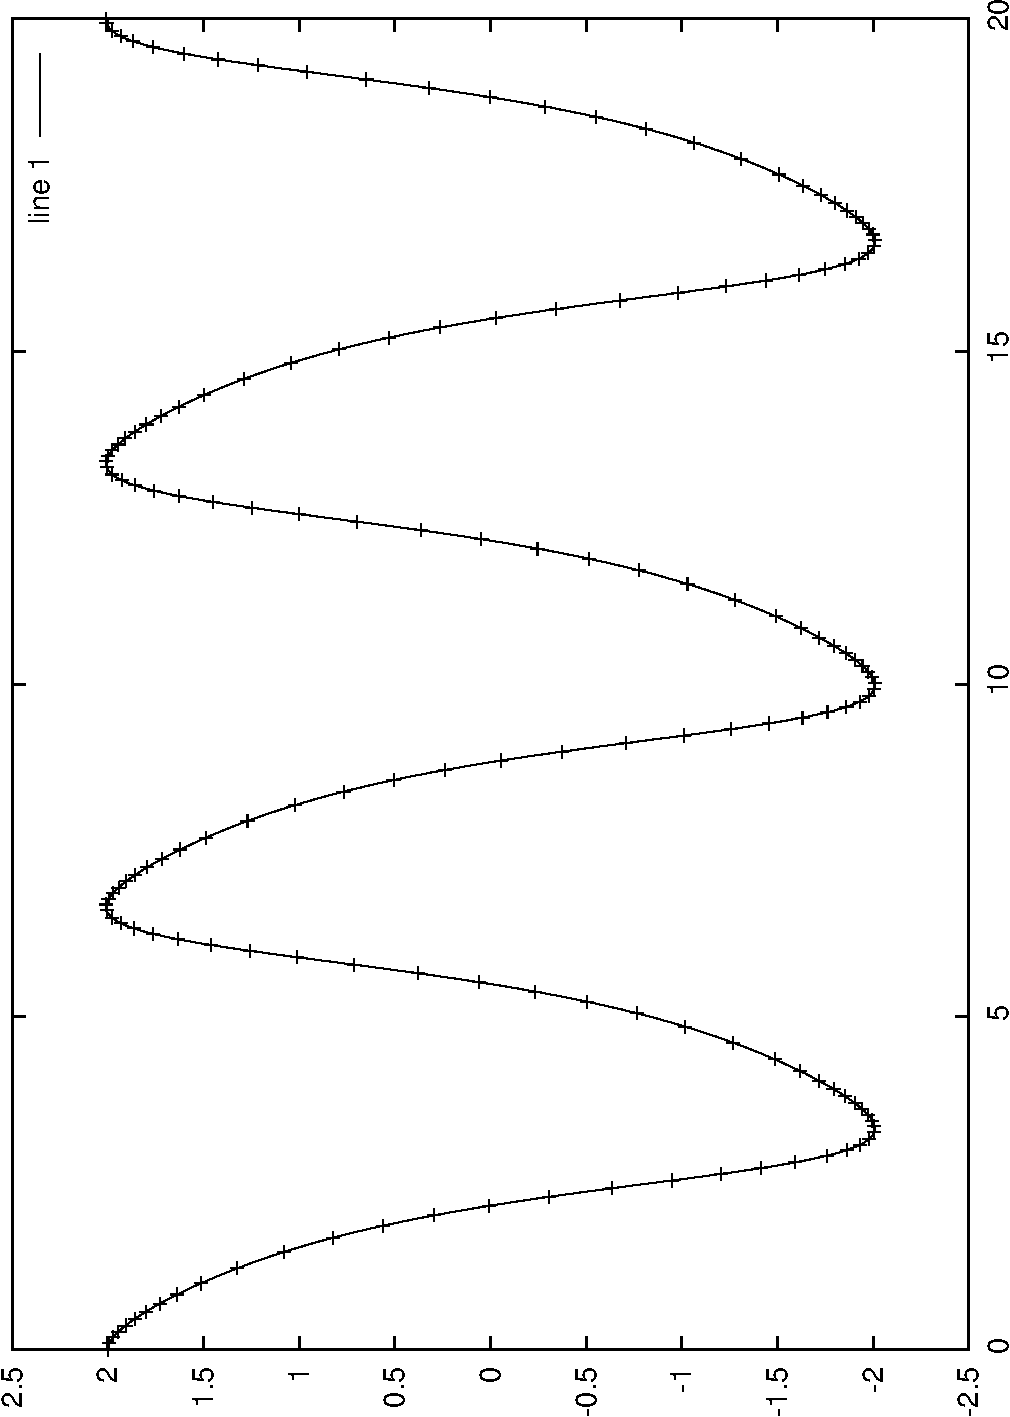
\includegraphics[%
  height=11cm,
  keepaspectratio,
  angle=-90]{figuras/comparisonode}


\caption{\label{cap:odenostiff}Solución de la ecuación de Van der Pol con
$\mu=1$}
\end{figure}



\subsubsection{Integración del problema stiff (\texttt{vdp1000}\index{vdp1000})}

Como los problemas stiff introducen gradientes elevados en la solución
el paso de integración de un esquema explícito se va haciendo tan
pequeño que su avance es demasiado corto. Es precisamente lo que ensayamos
en este caso. Si intentamos resolver la ecuación de Van der Pol con
$\mu=1000$ y $t\in[0,3000]$ mediante un esquema explícito:

\begin{itemize}
\item Octave
\end{itemize}
  \begin{verbatim}
>> lsode_options('integration method','non-stiff')

>> y=lsode('vdp1000',[0 2],linspace(0,3000,100000));
 \end{verbatim}
\begin{itemize}
\item Matlab
\end{itemize}
  \begin{verbatim}
>> [tout,xout]=ode45(@vdp1000,[0 3000],[2 0]); 
 \end{verbatim}
nos encontramos con la desagradable sorpresa de que el calculo no
termina nunca. Esto es porque la solución, aunque es regular, tiene
puntos con gradiente casi infinito.

La solución es utilizar un esquema implícito o semimplícito. Por ejemplo:

\begin{itemize}
\item Octave
\end{itemize}
  \begin{verbatim}
>> lsode_options('integration method','stiff')

>> ystiff=lsode('vdp1000',[2 0],linspace(0,20,1000));
 \end{verbatim}
\begin{itemize}
\item Matlab
\end{itemize}
  \begin{verbatim}
>> [tout,xout]=ode23s(@vdp1000,[0 3000],[2 0]);
 \end{verbatim}
Efectivamente, la solución demuestra por qué el problema es stiff
(Figura \ref{cap:odestiff}):

%
\begin{figure}[H]
\centering{}

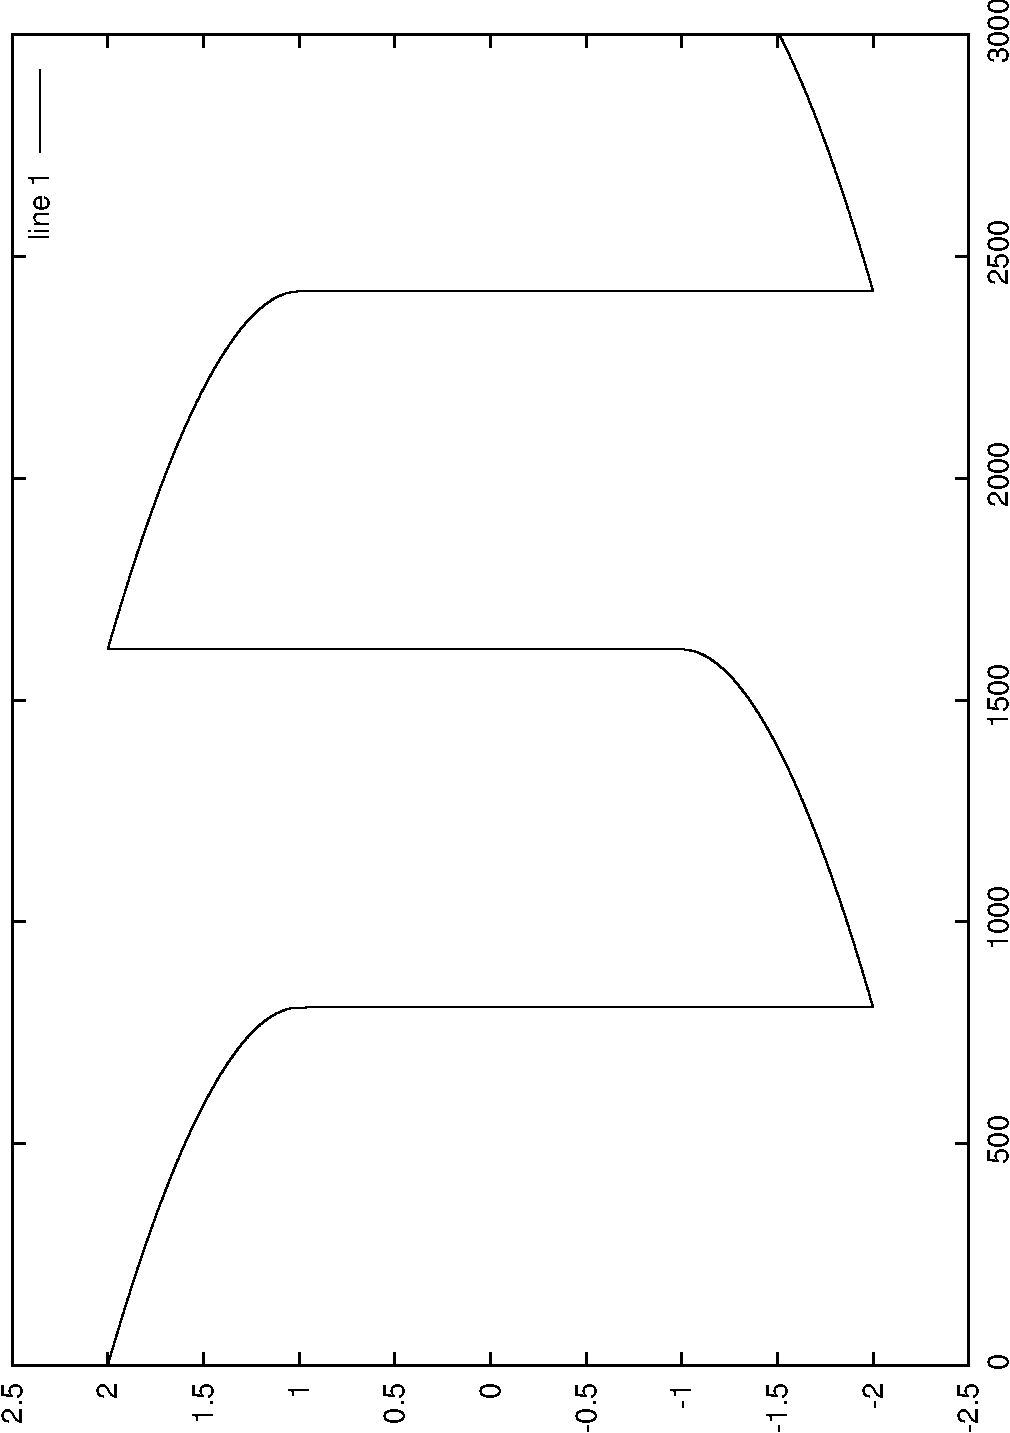
\includegraphics[%
  height=11cm,
  keepaspectratio,
  angle=-90]{figuras/comparisonodestiff}


\caption{\label{cap:odestiff}Solución de la ecuación de Van der Pol con $\mu=1000$}
\end{figure}



\subsection{Inestabilidades y caos\index{caos}.}

Uno de los casos en los que el cálculo numérico es una herramienta
imprescindible es en la resolución de ecuaciones diferenciales no
lineales, tanto ordinarias como en derivadas parciales. La no
linealidad de las ecuaciones hace que el carácter de los problemas de
evolución sea mucho más complejo que en el caso lineal. Uno de los
fenómenos observados es la aparición de caos.%
\footnote{Esta sección es sólo una pequeña introducción a los efectos
  del caos.  No soy un absoluto un experto en el tema pero se comenta
  en esta sección porque puede tener efectos desconcertantes en la
  solución. Pido disculpas si existe algun fallo garrafal en alguna de
  las afirmaciones.%
}

Supongamos que queremos resolver la ecuación del dipolo de
Rikitake\index{Rikitake} de ecuaciones:$$
\begin{array}{ccl}
  \dot x_{1} & = & -x_{1}+x_{3}x_{2}\\
  \dot x_{2} & = & -x_{2}+(x_{3}-3.75)x_{1}\\
  \dot x_{3} & = & 1-x_{1}x_{2}\end{array}$$
Despues de introducirlo en la función \texttt{rikitake.m:}

\begin{verbatim}
function xdot=rikitake(x,t)
%
% Ecuacion de la dinamo de Rikitake
%
xdot(1,1)=-x(1)+x(3)*x(2);
xdot(2,1)=-x(2)+x(1)*(x(3)-3.75);
xdot(3,1)=1-x(1)*x(2);
\end{verbatim}
Y resolver el problema utilizando la función \texttt{ode45} Octave%
\footnote{¿Por qué hemos tenido que utilizar el argumento adicional
  \texttt{ode\_fcn\_format}?% 
}:

  \begin{verbatim}
>> [t,x]=ode45(@rikitake,[0 300],[1 2 3],pair=0,ode_fcn_format=1);
plot(t,x(:,1),';x_1;',t,x(:,2),';x_2;',t,x(:,3),';x_3;')
\end{verbatim}
Nos encontramos con la desagradable sorpresa de que nuestra solución
es completamente errática (figura \ref{cap:rikitake2d}).

%
\begin{figure}[H]
  \centering{}

  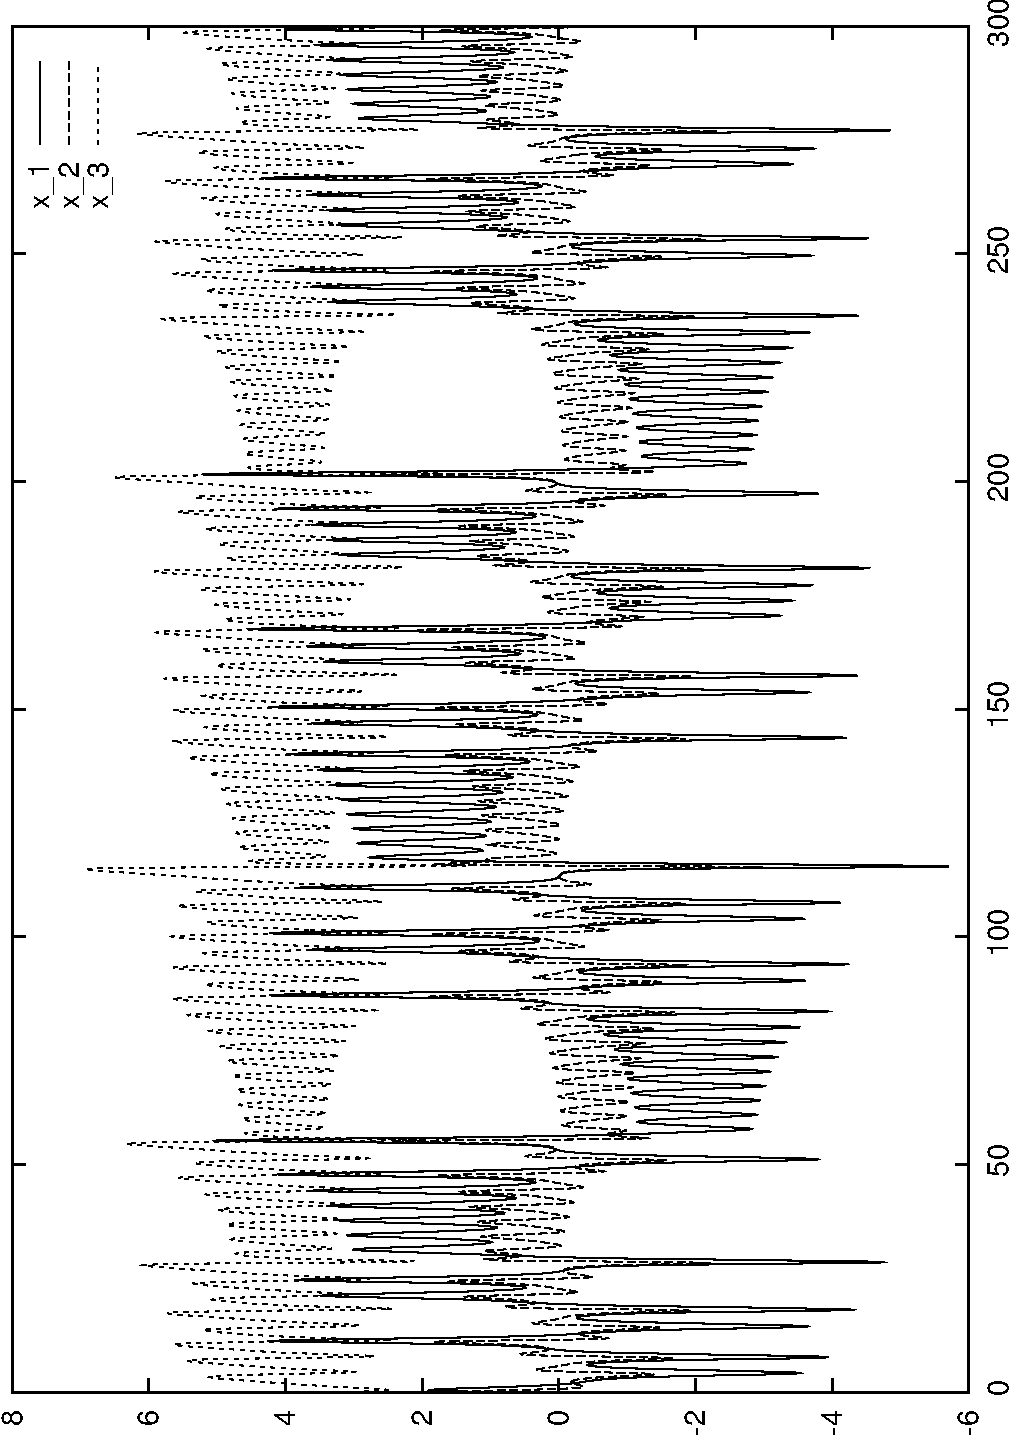
\includegraphics[%
  height=11cm,
  keepaspectratio,
  angle=-90]{figuras/rikitake}


\caption{\label{cap:rikitake2d}Solución del dipolo de Rikitake}
\end{figure}


A primera vista puede parecer que la solución está mal. Si representamos
exactamente el mismo resultado pero mediante una curva paramétrica:

  \begin{verbatim}
>> plot3 (x(:,1),x(:,2),x(:,3))
 \end{verbatim}
llegamos a la figura \ref{cap:rikirake3d}.

%
\begin{figure}[H]
\centering{}

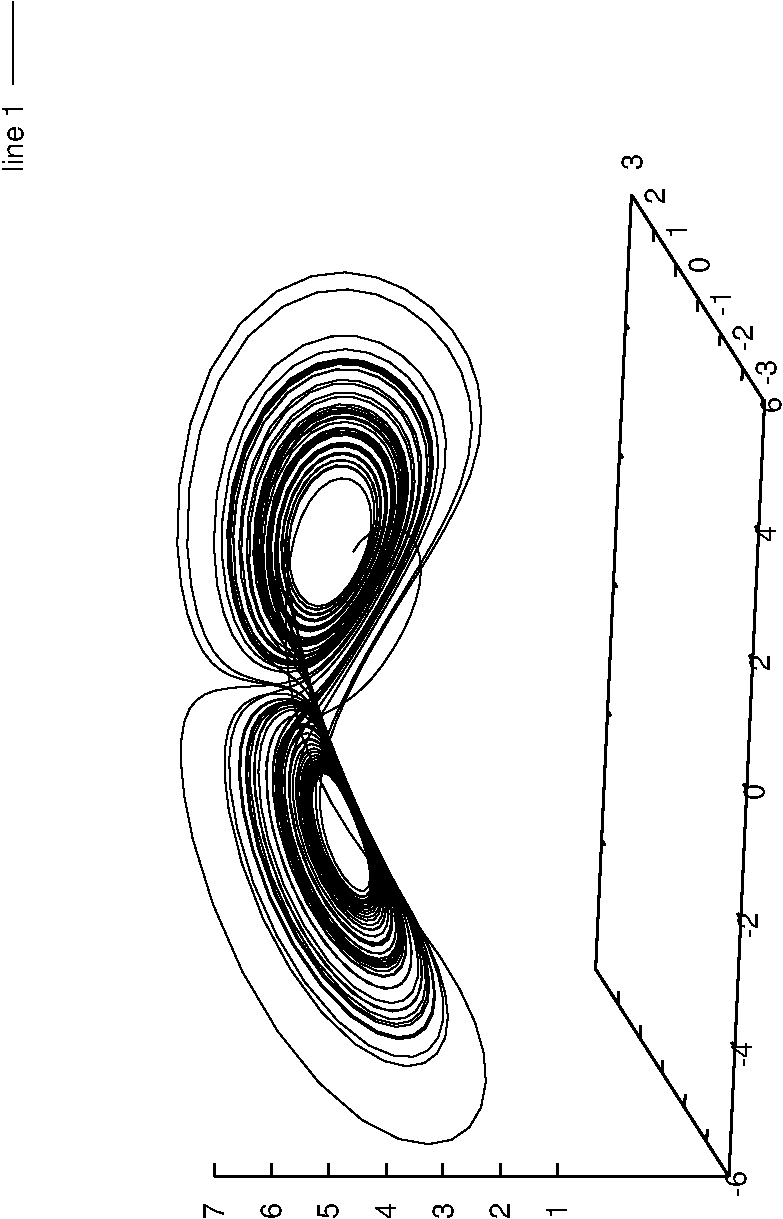
\includegraphics[%
  height=11cm,
  keepaspectratio,
  angle=-90]{figuras/rikitake3d}


\caption{\label{cap:rikirake3d}Curva solución del dipolo de Rikitake}
\end{figure}


De este ejemplo aprendemos que las ecuaciones diferenciales no lineales
pueden tener un comportamiento extraño. Un ejemplo claro de ello son
las ecuaciones de Navier Stokes. Si simplificamos las ecuaciones para
flujo incompresible nos encontraremos un término lineal (el viscoso)
y uno no lineal (el convectivo). El estudio analítico de estas ecuaciones
aún no ha llegado a la conclusión sobre la existencia y la unicidad
de la solución%
\footnote{El estudio de existencia y unicidad de la solución de las ecuaciones
de Navier Stokes para el caso incompresible es uno de los grandes
problemas no resueltos de las matemáticas.%
}, sin embargo se resuelven por métodos numéricos.

La turbulencia, uno de los fenómenos físicos más complejos, aparece
de forma espontanea cuando intentamos resolver las ecuaciones de N-S.
Parte de la disciplina de la CFD (Computational Fluid Dynamics) es
estudiar los flujos turbulentos a partir de la resolución numérica
de las ecuaciones de N-S.

La conclusión es que la integración numérica de ecuaciones diferenciales
es un problema complejo no sólo por la física del problema sino porque
además se suman muchos otros factores. En esta pequeña introducción
sólo hemos visto los problemas stiff y un caso muy sencillo de caos
pero los problemas pueden complicarse muchísimo más.


\section{Cálculo simbólico}

La afirmación repetida hasta la saciedad de que Matlab es un programa
\emph{estrictamente} de cálculo matricial no es del todo correcta.
Se basa en la aplicación del sentido crítico a una herramienta. La
versión completa de Matlab incluye el programa de cálculo simbólico
más utilizado actualmente, Maple. Los problemas generados por el uso
del cálculo simbólico en Matlab son dos:

\begin{enumerate}
\item Tenemos acceso al núcleo de cálculo de Maple, pero dicho acceso no
es completo. Podemos efectuar las operaciones básicas como derivar,
buscar primitivas, crear desarrollos de Taylor... Nunca dispondremos
de la potencia de este tipo de programas.
\item La arquitectura de matlab \textbf{no está pensada para el cálculo
simbólico}. Los programas de cálculo simbólico suelen incluir un interfaz
llamado \emph{notebook} que sirve para ver las fórmulas de entrada
y salida en una notación mucho más matemática. Las diferencias en
el diseño de un programa de cálculo numérico y otro de cálculo simbólico
son a mi parecer irreconciliables.
\end{enumerate}
Esto no significa que sea un crimen utilizar las funciones de cálculo
simbólico cuando uno disponga de ellas. Somos libres de hacer lo que
queramos pero debemos ser conscientes de hasta qué punto no estamos
utilizando la herramienta ideal para nuestro fín.

Octave también dispone de un soporte muy limitado para realizar operaciones
simbólicas. Se podría decir que lo único que puede hacer es derivar
y resolver sistemas de ecuaciones lineales. Tampoco parece que en
un futuro cercano estas funcines se amplíen hasta un soporte equivalente
al de Matlab. No son compatibles pero las funciones son tremendamente
parecidas.

Los siguientes apartados sirven como introducción general al uso de
variables simbólicas pero no conseguiremos más que arañar la superficie
del total de las posibilidades del toolkit.


\subsection{Definición de variables y funciones simbólicas}

\emph{Una de las diferencias más esenciales entre Matlab y Octave en
  lo que respecta a cálculo simbólico es que en Octave es necesario
  activar el toolkit con el siguiente comando}:

\begin{verbatim}
>> symbols
\end{verbatim}
Tanto en Matlab como en Octave el modo más fácil de definir una
variable simbólica es crear una variable que contenga un argumento
simbólico del mismo nombre:

\begin{description}
\item [sym\index{sym}]Define una variable que contiene un argumento
  simbólico.  Es muy recomendable que la variable y el argumento
  tengan el mismo nombre para evitar confusiones
\end{description}
\begin{verbatim}
>> x = sym('x')
\end{verbatim}
\begin{description}
\item [poly2sym\index{poly2sym}]Define un polinomio simbólico a partir
  de sus coeficientes.
\end{description}
\begin{verbatim}
>> poly2sym([1 2 3 -2 10])
ans =
10.0+(-2.0+x*(3.0+(2.0+x)*x))*x
\end{verbatim}

\subsection{Funciones simbólicas elementales.}

La aplicación de funciones elementales a variables simbólicas es completamente
distinta en Matlab y en Octave. Mientras Matlab no diferencia las
funciones simbólicas de las numéricas Octave prefiere llamarlas de
un modo distinto. Esta distinción suele ser que la primera letra de
la función es una mayúscula%
\footnote{Siempre viene bien recordar que la arquitectura de Matlab distingue
entre mayúsculas y minúsculas%
}. Entonces, para conseguir la función simbólica $\sin x$ en Matlab
haremos:

  \begin{verbatim}
>> x=sym('x')
x =
x
>> y=sin(x)
y =
sin(x)
 \end{verbatim}
Mientras que en Octave haremos lo siguiente:

  \begin{verbatim}
>> x=sym('x')
x =
x
>> y=Sin(x)
y =
sin(x)
 \end{verbatim}
En la colección podemos encontrar todas las funciones trigonométricas,
exponenciales, logaritmos...


\subsection{Operaciones simbólicas}

Casi todas las operaciones disponibles en el paquete simbólico de
Octave están dedicadas a la manipulación simbólica de polinomios (muy
interesante en el cálculo numérico). En cambio Matlab dispone de la
mayoría de las operaiciones simbólicas existentes... Derivadas, primitivas,
desarrollos en serie... La única función interesante en lo referente
a cálculo simbólico que tiene Octave es la siguiente:

\begin{description}
\item [subs\index{subs}]Substituye una o varias variables de una expresión
simbólica.
\item [collect\index{collect}]Agrupa los términos polinómicos en una variable
dada.
\item [expand\index{expand}]Desarrolla una expresión simbólica.
\item [differentiate\index{differentiate}]Sólo en Octave. Calcula la n-ésima
derivada de una expresión simbólica.
\end{description}
Función que en Matlab recibe un nombre distinto:

\begin{description}
\item [diff\index{diff}]Sólo en Matlab. Calcula la n-ésima derivada de
una expresión simbólica.
\end{description}
Matlab dispone además de las siguientes operaciones:

\begin{description}
\item [int\index{int}]Encuentra la primitiva de una función simbólica
\item [limit\index{limit}]Calcula el límite hacia un determinado valor
de una función simbólica.
\item [taylor\index{taylor}]Calcula el desarrollo en serie de Taylor respecto
a un punto dado de una función simbólica.
\item [symsum\index{symsum}]Calcula la suma de dos series.
\end{description}
Una de las pocas operaciones compatibles es la representación de una
curva determinada por una función simbólica:

\begin{description}
\item [splot\index{splot}]Dibuja la curva representación de una función
simbólica de una variable. El segundo argumento es un vector de dos
elementos con el intervalo de la variable independiente.
\end{description}
  \begin{verbatim}

 \end{verbatim}

%toolkits
%%%%%%%%%%%%%%%%%%%%%%%%%%%%%%%%%%%%%%%%%%%%%%%%%%
\chapter{Toolkits}
%%%%%%%%%%%%%%%%%%%%%%%%%%%%%%%%%%%%%%%%%%%%%%%%%%

Las funciones que que aparecen en este capítulo no son necesariamente
parte de un toolkit de Matlab. No es más que una clasificación artificial
de las funciones con una finalidad concreta que no justifica la creación
de un capítulo a parte. Esta sección es mucho menos amplia de lo que
debería, se ha sacrificado a propósito a favor de temas más básicos
como el cálculo el álgebra o el dibujo de gráficas. Mientras todo
lo escrito hasta aquí es casi definitivo este capítulo no se considerará
nunca como terminado.


\section{Estadística descriptiva y análisis de datos}

Matlab es un lenguaje muy utilizado en análisis de datos, tanto
experimentales como producidos por otros programas. En el caso de las
series de datos experimentales habrá que importar un archivo
almacenado en un formato compatible y asignar todos los valores a una
variable; más adelante aprenderemos a hacerlo.

Supongamos el caso ideal de que ya tenemos todos los datos cargados en
una variable. Matlab tiene una cantidad enorme de rutinas que
facilitan el análisis de datos de modo interactivo. las funciones son
tan de alto nivel que es posible sacar cualquier resultado secundario
sin necesidad de pensar un script; directamente con la consola. las
funciones más útiles son:

\begin{description}
\item [mean\index{mean}]Calcula la media de una muestra de datos:
  $\bar{x}=\frac{1}{n}\sum_{n=1}^{n}x_{i}$.
\item [std\index{std}]Calcula la desviación típica de una muestra de
  datos: $s=\sqrt{\frac{1}{n-1}\sum_{i=1}^{n}(x_{i}-\bar{x})^{2}}$.
\item [median\index{median}]Calcula la mediana de la muestra.
\item [min\index{min}]Valor mínimo de la muestra.
\item [max\index{max}]Valor máximo de la muestra.
\item [sort\index{sort}]Ordena los elementos de menor a mayor.
\item [center\texttt{\index{center}}]Resta el valor medio de la serie
  de datos.
\end{description}

\subsection{Ajuste de curvas por mínimos cuadrados.}

Supongamos que tenemos una serie de datos obtenidos mediante un
experimento y queremos hacer cálculos con ellos. El principal
impedimento es que ya no disponemos de una serie continua de datos
sino de medidas discretas.  Las dificultades que se presentan son
numerosas; no podemos poner dichos datos en un sistema de ecuaciones
no lineales porque no es diferenciable, tampoco en una ecuación
diferencial. La solución es convertir estos datos en una muestra
contínua que nuestras herramientas numéricas puedan manejar.

La práctica más común es la de utilizar un ajuste polinómico. El
polinomio resultante se obtiene resolviendo el problema de mínimos
cuadrados.  El grado del polinomio es uno de los datos que debemos
escoger. Suele ser una regla válida que polinomios de mayor órden
consiguen menor error pero no es siempre cierta. \textbf{Es bastante
  usual utilizar erroneamente el ajuste por mínimos cuadrados; sirven
  para crear un modelo polinómico de una función, no para conseguir
  una curva a través de unos puntos; para esto está la interpolación.}
Por ejemplo, supongamos que disponemos de la siguiente serie de datos:

\begin{center}\begin{tabular}{|c|c|}
    \hline 
    x&
    y\tabularnewline
    \hline
    \hline 
    0&
    2.0000\tabularnewline
    \hline 
    0.1&
    2.1850\tabularnewline
    \hline 
    0.2&
    2.2011\tabularnewline
    \hline 
    0.3&
    2.5762\tabularnewline
    \hline 
    0.4&
    2.5780\tabularnewline
    \hline 
    0.5&
    2.9711\tabularnewline
    \hline 
    0.6&
    2.7816\tabularnewline
    \hline 
    0.7&
    3.0766\tabularnewline
    \hline 
    0.8&
    2.8277\tabularnewline
    \hline 
    0.9&
    3.6763\tabularnewline
    \hline 
    1&
    3.6933\tabularnewline
    \hline
  \end{tabular}\end{center}

\begin{description}
\item [polyfit\texttt{\index{polyfit}}]Devuelve los coeficientes del
  polinomio del grado que queramos y soluciona el problema de ajuste
  por mínimos cuadrados.
\end{description}
Introducimos ahora las dos series de datos e intentamos ajustarlo por
mínimos cuadrados para crear un modelo \textbf{lineal} de los datos
adquiridos. Lo conseguimos con la siguiente líneas de código:

\begin{verbatim}
fit=polyfit(linspace(0,1,11),y,1)
fit=
  1.5928
  1.9828
\end{verbatim}
Ahora tenemos dos números en un vector llamado \texttt{fit}, este
vector son los dos coeficientes del polinomio que ajusta los datos;
una recta. Ahora representaremos gráficamente los datos del siguiente
modo

\begin{verbatim}
plot(linspace(0,1,11),y,'b*')
hold on
plot(linspace(0,1,11),polyval(fit,linspace(0,1,11)))
\end{verbatim}
El resultado es la figura \ref{cap:Ajuste por minimos cuadrados}

%
\begin{figure}[h]
  \centering{}

  \includegraphics[%
  width=10cm,
  height=12cm,
  keepaspectratio]{figuras/fitting}


\caption{\label{cap:Ajuste por minimos cuadrados}Ajuste por mínimos cuadrados
de una serie de puntos}
\end{figure}


Resolver un problema de mínimos cuadrados es en el fondo resolver
un problema mal condicionado. Si se plantean las ecuaciones del problema
llegamos a un sistema lineal mal condicionado. El criterio de resolución
suele ser el de minimizar el error cuadrático de la solución dada
(por eso el nombre de mínimos cuadrados). Este es exactamente el mismo
problema planteado en la pseudoinversa, operación que también se realiza
por mínimos cuadrados.

Nada nos obliga a ajustar los datos mediante un polinomio; la condición
de minimización del error cuadrático puede utilizarse con cualquier
función aunque siempre será más sencillo hacerlo con polinomios. Una
práctica muy habitual es utilizar un ajuste exponencial, táctica para
la que Matlab no ha escrito ninguna función. El motivo es bien sencillo,
si tenemos una nube de puntos que creemos sigue un modelo exponencial
lo único que debemos hacer es calcular el logaritmo de la serie de
datos para lo que recuperaremos automáticamente el ajuste polinómico.


\subsubsection{¿Qué calcula el ajuste polinómico por mínimos cuadrados?
  \label{sub:=BFQu=E9-calcula-el}}

Cuando hemos hablado de mínimos cuadrados en realidad nos referimos a
los Mínimos Cuadrados Lineales Generales. El problema planteado es el
de ajustar una serie de datos cualquiera a una función de la forma:

$$
y(x)=a_{1}+a_{2}x+a_{3}x^{2}+\ldots+a_{N}x^{N-1}$$

Este no es más que el tipo más sencillo de ajuste. Podríamos utilizar
también series de funciones armónicas o funciones arbitrarias de la
forma

$$
y(x)=\sum_{k=1}^{N}a_{k}X_{k}(x)$$

en las que $X$ representa una base de funciones. El objetivo es
minimizar el funcional error representado por la expresión

$$
E^2=\sum_{i=1}^{N}\left[
  \frac{y_{i}-\sum_{k=1}^{N}a_{k}X_{k}(x_{i})}{\sigma_{i}}\right]^{2}
$$

donde $\sigma$ es la desviación estándar de la muestra i-ésima. Esta
formulación permite generar una matriz para una aplicación lineal:

$$
A_{ij}=\frac{X_{j}(x_{i})}{\sigma_{i}}$$

Matriz que posee muchas más filas que columnas. La buena noticia es
que acabamos de generar un problema tan simple como una aplicación
lineal ($\mathbf{a}x=b$), la mala es que la matriz no es cuadrada y no
servirán los métodos de resolución convencionales. Una de las posibles
estrategias de resolución es utilizar una SVD para resolver el
sistema.

\section{Interpolación y aproximación de funciones}

La aproximación local o global de funciones es una parte esencial del
cálculo y del análisis.  Esta sección supone que ya conocemos los
desarrollos de Taylor o las transformadas de Fourier.  Algunos de los
métodos planteados no son más que la extensión discreta de métodos
comunes.

Aunque no sea del todo riguroso dividiremos este tema en tres partes
según las características del desarrollo de nuestros datos.  En
cálculo numérico siempre nos veremos obligados a describir una función
de un modo discreto, ya sea por el valor que toman en algunos puntos o
por los coeficientes de un desarrollo.  Dichas descripciones son más o
menos adecuadas según la finalidad que busquemos.

Hablaremos de la interpolación polinómica a trozos cuando sean dados
los valores de la función en unos puntos o nodos fijos.  Utilizaremos
funciones sencillas para intentar hallar una función continua que pase
por todos los puntos.  Hablaremos de interpolación polinómica cuando
queramos modelar una función conocida o desconocida mediante funciones
más simples buscando el mínimo error posible.  Se diferencia de la
anterior en que nuestro dato es una función y no una serie de puntos,
esto nos permitirá escoger los nodos para buscar el mínimo error de
interpolación.  Por último trataremos a parte los desarrollos en serie
de funciones sea cual sea la base (funciones armónicas, polinomios)

En el primer caso buscaremos convertir unos datos de naturaleza
discreta en una función continua, en el segundo y el tercer caso
intentaremos describir una función de un modo discreto, ya sea por sus
valores o por unos coeficientes, por ejemplo para hallarla cuando es
el resultado de una ecuación en derivadas parciales.

Los métodos numéricos no son exclusivos de cada uno de los objetivos,
los splines, por ejemplo, sirven tanto para hallar una curva contínua
como para describir una función mediante unos coeficientes.  El uso de
estas distinciones es que Matlab se basa más en la utilidad del método
numérico que en su naturaleza.  Si queremos splines para interpolar
utilizaremos una función distinta de la dedicada a hallar sus
coeficientes.

\subsection{Interpolación polinómica a trozos}

La interpolación polinómica a trozos será \emph{para nosotros} la
técnica de hallar una curva que pase por unos puntos dados.  Se dice
que es a trozos porque se utilizan polinomios de bajo orden definidos
a intervalos.

\begin{description}
\item [interp1\texttt{\index{interp1}}]Usa los puntos para interpolar
  en una dimension. Soprota interpolación discreta, lineal, cúbica,
  hermitiana y por splines cúbicos.
\end{description}
Un ejemplo gráfico es el siguiente script:

\begin{verbatim}
xf=0:0.05:10;yf=sin(2*pi*xf/5);
xp=0:10 ;yp=sin(2*pi*xp/5);
lin=interp1(xp,yp,xf);
spl=interp1(xp,yp,xf,'spline');
cub=interp1(xp,yp,xf,'cubic');
near=interp1(xp,yp,xf,'nearest');
title('Comparacion de las opciones de interp1')
plot(xf,yf,xf,lin,xf,spl,xf,cub,xf,near)
legend('real','lineal','splines','cubica','discreta')
\end{verbatim}
Cuyo resultado es la figura \ref{cap:Comparaci=F3n-de-los}.

%
\begin{figure}[h]
  \centering{}

  \includegraphics[%
  width=12cm,
  height=12cm,
  keepaspectratio]{figuras/figuraejemplo2}


  \caption{\label{cap:Comparaci=F3n-de-los} Comparación de los métodos
    de interpolación}
\end{figure}


\begin{description}
\item [interp2\texttt{\index{interp2}}]Interpolación polinómica
  bidimensional.
\end{description}
De entre todos los métodos de interpolación a trozos el más efectivo
suele ser siempre el uso de splines. Un spline es una curva cúbica; de
este modo reduciremos en gran medida el error en el caso que los
puntos \emph{sean de una función suave}, cosa que no sabemos. Cuando
interpolamos por trozos es importante conocer algo de información
sobre la función que representan, no sirve ninguna formula universal

Sería muy lógico en este punto plantearse la siguiente pregunta. ¿Por
qué escoger una función definida a intervalos y no un único polinomio
de grado igual al número de puntos menos 1? La respuesta aparece
cuando intentamos realizar el cálculo. Los polinomios de alto orden
tienen tendencia a oscilar en sus extremos, es el llamado fenómeno de
Runge.  Como patrón diremos que todo lo relacionado con polinomios de
alto orden suele acarrear problemas. Trataremos con más profundidad la
interpolación polinómica en un dominio finito en la sección
\ref{sub:Aproximación-de-funciones}.

\subsubsection{Splines}
\label{sec:splines}
La interpolación polinómica a trozos más común en Matlab es la
interpolación mediante splines.  Un spline es una curva definida
mediante polinomios en intervalos finitos, la interpolación será
entonces del orden que deseemos según el polinomio aunque lo más
frecuente será utilizar splines cúbicos.  Como en muchos otros casos
los splines no sirven únicamente para convertir en continua una serie
de datos discreta, función que cumple \texttt{interp1}.  Pueden servir
también para analizar más profundamente los datos estimando sus
derivadas e incluso para resolver ecuaciones en derivadas parciales.

Para quien desee algo de rigor matemático definimos un spline como el
conjunto de polinomios $p_j(x)$ que ajustan una determinada función
$f(x)$ en $[a,b]$, donde cada polinomio tiene validez en un intervalo
$\xi_j \in [a,b]$.  Además de imponer que la curva pase por todos los
puntos podemos imponer también que dichos polinomios se unan
suavemente al final de sus intervalos de definición.  Podemos
representar el conjunto mediante sus coeficientes y los nodos (
\emph{pp form})

$$p_j(x)=\sum_{i=1}^k(x-\xi_j)^{k-i}c_{ij}$$

o como B-spline, generalización de las curvas de Bézier.

Matlab, en su \emph{spline toolkit}, proporciona funiones para
calcular y evaluar con toda libertad los coeficientes de una
interpolación a trozos mediante splines, \emph{piecewise spline
  interpolation}.  Algunas de las funciones disponibles son las
siguientes:

\begin{description}
\item[spline\index{spline}] Llamada con dos parámetros retorna la
  matriz de coeficientes de la interpolación.  Llamada con tres
  parámetros retorna el valor de la interpolación en los valores
  dados.
\item[ppval\index{ppval}] Evalúa la interpolación mediante splines en
  los puntos dados dada su representación en coeficientes.
\item[csapi\index{csapi}] Define
\item[csape\index{csape}] Define
\end{description}

Un posible uso de los splines es la interpolación de curvas en más de
una dimensión.  Es un método muy habitual en diseño y es la base de
las herramientas de CAD con las NURBS (Non-Uniform Rational B-Splines).
Mediante puntos de control y unas pocas transformaciones geométricas
los splines definen casi todas las piezas producidas industrialmente.

\subsubsection{Regeneración de funciones mediante datos discretos}

Como ya hemos mencionado con anterioridad, uno de los problemas de
tratar con series discretas de datos es precisamente su no
continuidad.  Hay varias maneras de pasar los datos a una función y
hemos analizado que el ajuste polinómico no siempre es una buena
opción. Una solución más o menos universal es la de crear una función
mediante una interpolación y un function handle. Para ello sólo
tenemos que definir las series de datos y pasarlos como argumento a la
vez que definimos una variable independiente adicional. Por ejemplo,
suponemos que tenemos la siguiente serie de datos:

\begin{verbatim}
x=[1 2 3 4 5 6 7 8]
y=[2 4 3 5 4 6 5 7]
\end{verbatim}
Y queremos generar una función que sea capaz de proporcionar los datos
de forma continua. La solución es la creación del siguiente function
handle:

\begin{verbatim}
>> newfunc=@(z) interp1d([1 2 3 4 5 6 7 8],...
    [2 4 3 5 4 6 5 7],z,'spline');
\end{verbatim}

A todos los efectos esto es una nueva función que pasa por todas las
parejas de puntos $(x,y)$:

\begin{verbatim}
>> newfunc(3.443)
ans = 3.9162
\end{verbatim}

La técnica de reducir variables mediante function handles no es válida
en Octave, donde los FH son estrictamente funciones independientes.


\subsection{Transformadas rápidas de Fourier}

Un desarrollo posible de una función \textbf{periodica} es el
desarrollo de Fourier. En él las funciones ortogonales que nos sirven
de base son funciones armónicas que llamaremos $\Phi_{k}$. El
desarrollo de la función $u$ es entonces:
$$u=\sum_{k=-\infty}^{k=\infty}\hat{u}\Phi_{k}.$$ donde $\hat{u}$ son
los coeficientes de Fourier que \textbf{suelen ser números complejos}.
Si la función admite el desarrollo anterior también admitirá una
\emph{serie truncada de fourier}. Esta serie tiene la forma:
$$P_{N}u=\sum_{k=-\frac{N}{2}}^{k=\frac{N}{2}-1}\hat{u}_{k}e^{ikx}$$
que constituye la serie truncada de Fourier de orden $N$. Los
coeficientes se calculan exactamente del mismo modo que la anterior
con la diferencia que truncamos el desarrollo a partir de un cierto
número de onda.  En el cálculo numérico nunca trabajaremos con
desarrollos con una cantidad infinita de términos; esto es dominio del
cálculo simbólico.

Si aproximamos la función inicial por un polinomio interpolante
definido a partir de una serie de puntos llegamos a la \emph{serie
  discreta de Fourier}. Se dice discreta porque tiene como datos los
puntos en los que se evalúe la función. Exactamente del mismo modo
podríamos estar trabajando con una serie de puntos experimentales.
Esto generará un desarrollo discreto porque sólo con unos cuantos
puntos no tenemos suficiente información como para llegar a una serie
infinita.

Como estamos obteniendo toda la información posible normalmente se
habla de \emph{transformada discreta de Fourier}. El algoritmo para
calcularla es la \emph{t}ansformada \emph{rápida de Fourier} o
\emph{Fast Fourier Transform} (FFT).

\begin{description}
\item [fft\texttt{\index{fft}}]Aplica la transformada rápida de
  Fourier a una serie de puntos utilizando como funciones base
  $\Phi_{x}(x)=e^{ikx}$.
\item [ifft\index{ifft}]Calcula la antitransformada rápida de Fourier.
\end{description}
Las fft's se usan muchísimo en los métodos espectrales, resolución de
ecuaciones en derivadas parciales lineales y no lineales, análisis de
datos y filtrado de señales. Muchos de los problemas de la física con
condiciones de contorno periodicas son mucho más sencillos en su
formulación espectral.%
\footnote{La gran ventaja de las transformadas rápidas de Fourier es
  que son una operación especialmente rápida cuando tenemos series de
  $2^{n}$ puntos. En estos casos se hacen del órden de $N\log N$
  operaciones para calcularla. Esto las hace muy útiles en la
  resolución de ecuaciones en derivadas parciales lineales (ecuación
  de ondas) o por métodos espectrales. Un caso especialmente
  importante es el de la ecuación de Poisson
  ($\nabla^{2}\phi=f(\vec{x})$).

  Supongamos que tenemos las ecuaciones de Navier-Stokes en dos
  dimensiones.  Se demuestra que se pueden reescribir en función de
  $\omega$ y de $\psi$, la vorticidad y la función de corriente de la
  siguiente manera:
$$ \frac{\partial\omega}{\partial
  t}+\frac{\partial\omega}{\partial x}\frac{\partial\psi}{\partial
  y}-\frac{\partial\omega}{\partial y}\frac{\partial\psi}{\partial
  x}=\frac{1}{Re}\nabla^{2}\omega$$
  $$
  \nabla^{2}\psi=-\omega$$ Imaginemos entonces que queremos resolver
  un problema de turbulencia 2D isótropa con condiciones de contorno
  periódicas. Esto nos obliga a resolver una ecuación de Poisson por
  cada paso temporal, operación bastante costosa porque requiere la
  inversión de una matriz. Podemos ahorrarnos gran cantidad de
  operaciones si hacemos la transformada de Fourier de la segunda
  ecuación:$$
  \frac{\partial^{2}\hat{\psi}(i,j)\exp(\imath(kx+ly))}{\partial
    x^{2}}+\frac{\partial^{2}\hat{\psi}(i,j)\exp(\imath(kx+ly))}{\partial
    y^{2}}=-\hat{\omega}\exp(\imath(kx+ly))$$
  $$
  \hat{\psi}(i,j)(k^{2}+l^{2})=\hat{\omega}(i,j)$$ Que es un sistema
  de ecuaciones de resolución trivial. Acto seguido hacemos la
  antitransformada de los coeficientes $\hat{\psi}(i,j)$ y ya podemos
  pasar al paso de la ecuación parabólica.%
}

Disponemos también de otras funciones que encapulan tareas comunes en
las que están involucradas transformadas de fourier

\begin{description}
\item [fftshift\index{fftshift}]Mueve el primer número de onda
  (frecuencia cero) al centro del espectro.
\item [fftfilt\index{fftfilt}]Aplica directamente un filtro espectral.
\item [fft2\index{fft2}]Transformada rápida de Fourier bidimensional.
  También disponemos de una antitransformada para esta función
\item [fftn\index{fftn}]Transformada rápida de Fourier n-dimensional.
  Existe \texttt{ifftn}.
\end{description}
Las librerías de transformadas rápidas de Fourier suelen disponer de
transformadas del seno y del coseno para cubrir los casos de
condiciones de contorno no periodicas. Los drivers para estas
bibliotecas no son tan completos en Matlab y tendremos que convertir
la transformada exponencial en transformada de seno o de coseno
manualmente.


\subsection{Aproximación de
  funciones\label{sub:Aproximación-de-funciones}}

Esta técnica, aunque coceptualmente muy parecida a la interpolación
polinómica a trozos, suele tener usos completamente distintos. La
aproximación de una función o de una serie de puntos por un único
polinomio en un dominio dado se acerca más al desarrollo en serie de
Fourier que a la interpolación polinómica a trozos. Los polinomios de
Lagrange, de Legendre o de Chebyshev fueron creados para desarrollar
funciones continuas en dominios finitos mediante una base polinómica.
Tienen un uso esencial en la evaluación de funciones complejas en
dominios finitos y en los métodos espectrales de resolución de
ecuaciones en derivadas parciales.

La interpolación polinómica no suele utilizarse para ajustar una serie
de puntos dados por culpa del fenómeno de Runge. Supongamos que
tenemos la siguiente serie de puntos $y$ en función otra serie
equiespaciada de puntos $x$.

\begin{verbatim}
x =
 Columns 1 through 8:
 -1.00000  -0.87500  -0.75000  -0.62500  -0.50000  -0.37500  -0.25000  -0.12500
 Columns 9 through 16:
  0.00000   0.12500   0.25000   0.37500   0.50000   0.62500   0.75000   0.87500
 Column 17:
  1.00000
y =
 Columns 1 through 8:
 0.058824  0.075472  0.100000  0.137931  0.200000  0.307692  0.500000  0.800000
 Columns 9 through 16:
 1.000000  0.800000  0.500000  0.307692  0.200000  0.137931  0.100000  0.075472
 Column 17:
 0.058824
\end{verbatim}
Supongamos ahora que queremos ajustarla por un polinomio de grado
$N-1$ suponiendo $N$ el número de puntos de la serie. El polinomio
será entonces:
$$ p(x)=\sum_{i}^{N}a_{i}x^{i-1}$$
problema que se cerrará con la condición de que $p(x_{i})=y_{i}$.  Al
final se llega a la misma ecuación de siempre: $Ac=y$ donde $A$ es
la matriz de Vandermonde generada con los puntos $x_{i}$, $c$ el
vector de incógnitas de los coeficientes y $y$ el vector de puntos de
la serie $y_{i}$. El vector de coeficientes se genera con este código:

\begin{verbatim}
>> c=vander(x) \y'
c =
    6.4739e+03
    3.6848e-11
   -2.1040e+04
   -1.0123e-10
    2.7271e+04
    1.0430e-10
   -1.8231e+04
   -5.0934e-11
    6.8268e+03
    1.2373e-11
   -1.4741e+03
   -1.4184e-12
    1.8795e+02
    6.5051e-14
   -1.5402e+01
   -8.4500e-16
    1.0000e+00
\end{verbatim}
Si representamos este polinomio de orden 16 con los puntos que tiene
interpolar junto con la función solución
$y(x)=\frac{1}{1+16x^{2}}$(figura \ref{cap:runge}):

%
\begin{figure}[h]
  \centering{}

  \includegraphics[%
  width=10cm,
  height=12cm,
  keepaspectratio]{figuras/interpeq}


  \caption{\label{cap:runge}Demostración del fenómeno de Runge}
\end{figure}


Como vemos, la función interpolante cumple los requisitos impuestos,
pasa por todos los puntos; pero no hace nada más bien. ¿Cuál es
entonces el problema? ¿Qué hay que hacer para solucionarlo? La
interpolación polinómica es un problema global, es decir, intenta
aproximar toda una función con una cantidad limitada de datos (los
puntos de los que tenemos valores). A la función interpolante los
árboles no le dejan ver el bosque, si quiere ajustar con unos puntos
dados (nodos) es incapaz de capturar la función de la que provienen.

La solución es comprender las implicaciones globales del problema.  Ya
no estamos intentando hacer pasar una curva por una serie de puntos,
estamos intentando resolver la aproximación de la misma curva. La
solución la encontramos desde el punto de vista global... ¿Por qué los
nodos deben ser equiespaciados? ¿Y si acercamos los nodos entre ellos
(clustering) en las zonas donde los errores son más elvados?  Sean
cuales sean los tipos de polinomios que utilicemos así como el orden
del que sean hay nodos más adecuados para minimizar el error del
problema global, por ejemplo los nodos de Chebyshev de la forma:
$$x_{j}=cos(j\pi/N),\qquad j=0,1,...,N$$
puntos de Chabyshev-Lobatto o puntos extremos de Chebyshev. Esta
formula es la proyección de los puntos equiespaciados en una
circunferencia de radio unidad en el eje de abcisas. Si ahora en vez
utilizar los nodos equiespaciados utilizamos los nodos óptimos de
Chebyshev llegamos a que el polinomio de interpolación es
sensiblemente mejor (figura \ref{cap:chebyshev}):

%
\begin{figure}[h]
  \centering{}

  \includegraphics[%
  width=10cm,
  height=12cm,
  keepaspectratio]{figuras/chebyshevnodes}


  \caption{\label{cap:chebyshev}Uso de los nodos óptimos de Chebyshev
    para reducir el error de interpolación}
\end{figure}


Vemos entonces que recurrir a una elección óptima de nodos permite
utilizar polinomios como base de desarrollos de funciones con un error
más que aceptable con todas las ventajas que implica trabajar con
polinomios en nuestros cálculos.

\begin{description}
\item [Importante:]La interpolación polinómica es un problema global.
  No depende únicamente del número de puntos sino de su elección.
\end{description}
Una demostración de hasta dónde llega la importancia de elegir bien
los nodos es pensar que el error que se comete con un polinomio de
grado mayor no necesariamente se reduce con lo que estamos malgastando
tiempo y potencia de cálculo sin ganar precisión. Hay que hacer las
cosas con cuidado.


\section{Resolución de ecuaciones no lineales y optimización.}

Este apartado merece un pequeño comentario de entrada. Matlab posee
una más que amplia selección de funciones orientadas a la
optimización.  Matlab contiene funciones para hacer casi todo lo
imaginable como buscar ceros de funciones n-dimensionales y no
lineales, mínimos de funciones condicionados, programación
cuadrática... El gran problema es que todas estas herramientas están
en un toolkit que no forma parte de la instalación básica del
programa. En el caso que estemos delante de una versión comercial o de
estudiante del Matlab es posible que no dispongamos de ninguna de las
funciones anteriormente mencionadas.

No tiene mucho sentido entrar los detalles del Optimization Toolkit
porque la ayuda en formato HTML que se incluye en el paquete es más
que suficiente. Se podría decir que es una buena introducción a la
optimización en general.

Este tema es difícil de encajar en el planteamiento general del libro.
Siempre hemos buscado un planteamiento agnóstico respecto a los dos
intérpretes muy difícil de mantener en este caso. Octave sólo contiene
las funciones básicas de optimización, la colección es pobre si se
compara con el Optimization Toolkit; pero en la mayoría de los casos
es más que suficiente.

Veremos entonces sólo una introducción básica a la optimización,
minimización de funciones, programación lineal y no lineal y búsqueda
de raíces de sistemas de ecuaciones no lineales.


\subsection{Resolución de ecuaciones no lineales. Root finding.}

La resolución de sistemas de ecuaciones no lineales podría
considerarse como una disciplina independiente de la optimización.
Algunos de los métodos de resolución no tienen absolutamente nada que
ver con los algoritmos de minimización de funciones. Sin embargo hemos
decidido mantener un órden consistente con el de los paquetes de
funciones de Matlab.

Root finding es el término inglés para la práctica de la resolución de
una ecuación que no tiene una solución analítica o con una solución
exacta demasiado costosa de encontrar. Fue uno de los primeros casos
en los que se aplicó el cálculo numérico porque es donde se hace
imprescindible.

Todos los métodos se basan en la aproximación mediante un desarrollo
en serie de la función en un punto inicial. Lo que los diferencia es
el tipo de desarrollo y cómo aproximan la función en el punto.  El
método más básico de todos es el método de \emph{Newton} que se basa
en la aproximación lineal de la función en cada punto para obtener la
siguiente raíz para iterar. El método de la secante no es más que una
aproximación grosera de la derivada mediante dos puntos. Luego nos
encontramos con los métodos \emph{Regula-falsi}, \emph{Ridders}...  o
más sofisticados como el \emph{Van Wijngaarden-Dekker-Brent}.

Todos los métodos se usan de la misma manera, se les da una función,
un punto inicial y se cruzan los dedos. Lo único que debemos saber del
\emph{Root finding} en Matlab es que todo lo lleva la función...

\begin{description}
\item [fzero\index{fzero}]Busca la solución más cercana al punto
  inicial dado de cualquier ecuación dada.
\end{description}
Lo único que debemos recordar es que como cualquier función a la que
hay que dar otra función como argumento nos obligará a utilizar un
function handle. Por ejemplo, queremos encontrar el cero de la
siguiente ecuación:
$$ \ln x-\sin x=0$$
Esta ecuación no tiene una solución analítica con lo que el uso del
cálculo numérico se hace imprescindible. Suele ayudar representar
gráficamente las dos funciones (figura
\ref{cap:Representación}) para saber si se cruzan en algún
punto; si buscamos una solución inexistente es probable que el método
nos devuelva soluciones complejas o espúreas.

%
\begin{figure}[h]
  \centering{}

  \includegraphics[%
  width=12cm,
  keepaspectratio]{figuras/fzero}


  \caption{\label{cap:Representación}Representación de las
    funciones a resolver.}
\end{figure}


La función que se resolverá será siempre de la forma $f(x)=0$, de modo
que nuestro function handle será:

  \begin{verbatim}
>> eq=@(x) log(x)-sin(x);
>> sol=fzero(eq,1);
>> sol
sol =
    2.2191 
\end{verbatim}
que es consistente con la solución intuida basándonos en la gráfica.

Una más que buena práctica es pedir una solución dentro de un
intervalo puesto que en muchos casos las ecuaciones no lineales pueden
tener varias e incluso infinitas soluciones. Sólo hay que cambiar el
punto inicial de iteración por un intervalo de búsqueda:

  \begin{verbatim}
>> eq=@(x) log(x)-sin(x);
>> sol=fzero(eq,[1 4]);
>> sol
sol =
    2.2191 
\end{verbatim}

\subsubsection{Más incompatibilidades entre Matlab y Octave.}

En la versión 2.1 de Octave el soporte para los function handles es
bastante limitado. Muchas de las funciones, sobretodo las que no son
más que llamadas a rutinas en fortran o C, deben obtener las funciones
por su nombre y no mediante un function handle. La función
\texttt{fzer}o en Octave es una víctima bastante desafortunada de esta
limitación.  Si intentamos resolver la ecuación anterior por el primer
método propuesto recibiremos un error, a priori incomprensible,
mientras que con el segundo script llegaremos a la solución.

El motivo es el exótico comportamiento de \texttt{fsolve} en Octave.
Si le pasamos sólo un parámetro, \texttt{fzero} llamará a la función
\texttt{fsolve} de la que hablaremos en el siguiente apartado.
\texttt{fsolve} no tiene soporte para function handles de modo que
tendremos que pasarle la función por su nombre despues de haberla
definido, por ejemplo:

  \begin{verbatim}
>> function y=eq(x)
... y=log(x)-sin(x);
... end
>> fzero('eq',1)

ans = 2.2191
\end{verbatim}
Tampoco es una gran dificultad añadida ya que Octave soporta la
definición de funciones mediante el intérprete a diferencia de Matlab.
En cambio, si definimos un intervalo de búsqueda de soluciones sí le
podremos pasar un function handle como argumento porque usa un método
de resolución alternativo%
\footnote{\texttt{fsolve} utiliza el método Powell mientras que
  \texttt{fzero} utiliza un método Brent.%
}:

  \begin{verbatim}
>> eq1=@(x) log(x)-sin(x);
>> fzero(eq1,[1,4])
ans = 2.2191 
\end{verbatim}

\subsection{Búsqueda de soluciones de sistemas de ecuaciones no
  lineales.}

Se define como solución de un sistema de ecuaciones como la $x$ que
cumple:\[ \mathbf{f}(x)=0\] siendo $\mathbf{f}$ la función vectorial
representa al sistema.

El objetivo de la búsqueda de soluciones de sistemas de ecuaciones no
lineales es siempre el mismo. Llegar a una solución válida del sistema
con el mínimo coste computacional posible. La no linealidad de las
ecuaciones puede provocar todo tipo de catástrofes como la no
convergencia o que el error se dispare hacia el infinito. Siempre se
parará automáticamente la iteración y se nos dará un mensaje de error.
El coste computacional es una complicación menor. Depende de dos
aspectos, la elección del punto inicial y el algoritmo de evaluación
del gradiente de la función.

Los métodos más sencillos de resolución de ecuaciones no lineales se
basan en la aproximación lineal de la función en un punto. Si hacemos
el desarrollo de Taylor de primer orden en el punto inicial tenemos
que:$$ \mathbf{f}(x)=\mathbf{f}(x_{0})+(x-x_{0})\mathbf{J}(x_{0})$$

fórmula a la que le siguen términos de mayor órden.
$\mathbf{J}(x_{0})$ es el gradiente de la función evaluado en el punto
$x_{0}$. Si suponemos que el resultado de la aproximación es la
verdadera raíz de nuestra función:
$$
\mathbf{f}(x_{0})+(x-x_{0})\mathbf{J}(x_{o})=0$$ obtendremos el
siguiente punto de la iteración, en este caso $x=x_{1}$:
$$x_{1}=x_{0}-\mathbf{J}^{-1}(x_{0})\mathbf{f}(x_{0})$$


Iteración que se llevará a cabo hasta que se una norma de la solución
sobrepase una cota de error. Este método es conocido como
\emph{Newton-raphson}.  Esto nos recuerda que una de las operaciones
con mayor coste computacional es precisamente la inversión de una
matriz. Además la matriz es el gradiente de la función en un punto,
gradiente que puede ser en algunos casos casi imposible de calcular.
Nos encontramos ante el problema de evaluar de una manera óptima un
gradiente para luego evaluarlo e invertirlo. Todo esto considerando
que el punto inicial nos lleve más o menos directamente a la solución
que buscamos.

Nada de esto debe hacernos perder la referencia de que lo realmente
importante de los métodos de resolución es la facilidad con la que
converjan a una solución más que la rapidez con que lo hagan. Al igual
que en el caso unidimensional, Matlab apuesta por la simplicidad.  La
función que nos realizará la tarea es:

\begin{description}
\item [fsolve\index{fsolve}]Busca una solución de un sistema de
  ecuaciones dado. Esta función es diferente según se use en Matlab o
  en Octave; la versión de Matlab llamará al sistema de ecuaciones
  mediante su nombre o con un function handle mientras que la versión
  de Octave sólo podra llamarlo por nombre.
\end{description}
Las diferencias entre ambas sólo se manifiestan en el modo en el que
llamaremos a la función, no en el modo en el que la definiremos porque
es imposible expresar todo un sistema de ecuaciones sólo con un
function handle. Será imprescindible definir una función propiamente
dicha lo que en Matlab significará crear un archivo de función.


\subsubsection{Algunas de las cosas que pueden salir mal}

Resolver ecuaciones escalares no lineales o sistemas de ecuaciones no
lineales no es numéricamente muy complejo, pero los problemas son muy
a menudo mal condicionados. Infinidad de factores pueden llevarnos a
soluciones erróneas o a problemas de convergencia. Algunos de ellos
son muy simples como el siguiente:

  \begin{verbatim}
>> eq=@(x) log(x)-sin(x);
>> fzero(eq,[0 4])
Warning: Log of zero.
> In @(x) log(x)-sin(x)
  In fzero at 218
??? Error using ==> fzero
Function values at interval endpoints must be finite and real.
\end{verbatim}
Obviamente debido a que $\ln0=-\infty$.

Otros problemas debidos a la convergencia pueden ser un auténtico
dolor de cabeza


\subsection{Minimización de funciones.(+)}


\subsection{Minimización de funcionales.(+)}

%temas avanzados
%%%%%%%%%%%%%%%%%%%%%%%%%%%%%%%%%%%%%%%%%%%%%%%%%%

\chapter{Temas avanzados}

%%%%%%%%%%%%%%%%%%%%%%%%%%%%%%%%%%%%%%%%%%%%%%%%%%

Este capítulo nace de la necesidad de recojer todos los argumentos no
necesariamente ligados al uso de Matlab. La mayoría de ellos están
relacionados con la programación general o en cálculo numérico, sin
embargo son de gran utilidad para escribir buenos programas. La teoría
que contiene este capítulo es de un nivel mucho más elevado al resto,
estais avisados; esto no significa que todo esté explicado del modo
más sencillo posible.

\section{Aumentar la calidad del código escrito en Matlab}

Que el código funcione no suele ser suficiente. Debemos intentar en
cualquier caso escribir código de calidad, debemos convertir en
hábitos ciertas prácticas de programación orientadas a hacer más fácil
el uso de las funciones y los scripts. No todo termina en escribir una
pequeña ayuda en cada función. Hay estrategias muy útiles para
aumentar significativamente la potencia del código escrito sin
necesidad de aumentar el esfuerzo. Debemos entender que si Matlab es
una plataforma de desarrollo rápido de aplicaciones dispondrá de
funciones para escribir código de un modo más eficiente.

\subsection{Vectorizar, la clave para aumentar la velocidad}

Hay muchas maneras de asignar un argumento a una variable. Cuando se
crearon los ordenadores y empezaron a surgir los lenguajes de
programación casi todos los procesos eran escalares. Todo estaba
gobernado por operaciones lógicas que operaban unidades muy pequeñas
de memoria.  A medida que los ordenadores iban creciendo en potencia y
versatilidad se empezó a pensar en una manera más eficiente de
calcular. Uno de los conceptos era la vectorización.\footnote{ Un
  nombre propio en la arquitectura de ordenadores es Seymour Cray, su
  biografía está íntimamente ligada al los ordenadores vectoriales.
  Su influencia es tremenda en el campo de la computación a gran
  escala. }

Se dice que una operación es escalar cuando se hace elemento a
elemento.  Una suma escalar de dos vectores es tomar los elementos de
cada uno de ellos, sumarlos y asignar el resultado a un tercer vector.
Una operación es vectorial cuando se hace por bloques mayores en la
memoria.  Una suma vectorial de dos vectores sería tomar partes del
los vectores o los vectores enteros y sumarlos de golpe.

Los compiladores modernos son capaces de vectorizar automáticamente.
Advierten que dos bucles pueden combinarse perfectamente y realizan la
operación por bloques ahorrando memoria y tiempo de cálculo. Como
Matlab es un programa secuencial carece de esta capacidad de
optimización.  Si nosotros le pedimos un bucle con operaciones
escalares lo va a realizar sin ningún tipo de optimización. Si en
cambio asignamos operamos las matrices mediante la notación matricial
y las submatrices Matlab sí va a ser capaz de vectorizar la operación.

En la sección \ref{sub:El-truco-m=E1s} explicaremos la importancia que
todas estas consideraciones tienen sobre la velocidad de ejecución.

\subsubsection{\label{sub:El-truco-m=E1s}El truco más importante de la
  programación en Matlab}

El truco más importante para que nuestros scripts tengan una velocidad
aceptable es evitar los bucles con contador. Es la estructura más
lenta que existe en el lenguaje. El siguiente ejemplo nos ayudará a
entenderlo perfectamente. Crearemos dos matrices de números aleatorios
y las sumaremos creando una tercera matriz. Primero lo haremos
mediante un bucle que sume con dos índices y luego utilizando el
operador suma elemento a elemento. Utilizaremos la función
\texttt{rand} para crear las matrices y la pareja \texttt{tic} y
\texttt{toc} para calcular el tiempo de cálculo.

\begin{verbatim}
>> a=rand(66); #matriz de 66 x 66
>> b=rand(66);
>> tic;for i=1:66;for j=1:66;c(i,j)=a(i,j)+b(i,j);end;end;toc
ans = 0.17925
>> tic;c=a.+b;toc
ans = 0.00058100
\end{verbatim}
Donde el número que obtenemos como resultado es el tiempo transcurrido
entre la llamada de \texttt{tic} y la de \texttt{toc}. La diferencia
entre los dos métodos es de%
\footnote{El ordenador con el que han sido efectuadas las pruebas es
  un Athlon XP 2600+ (1.920 GHz, bogomips=3301.37) con 512 Mb de RAM a
  400 MHz y Octave 2.1.72. Matlab es ligeramente más rápido con el
  manejo de bucles aunque de ningún modo se acerca a la velocidad de
  los operadores matriciales. Con la optimización máxima Matlab y
  Octave tienen resultados equivalentes. Las pruebas se han efectuado
  diez veces y se da el tiempo medio de la muestra.%
}:

\begin{verbatim}
>> 0.17925/0.00058500
ans = 306.41
\end{verbatim}
Utilizar los operadores matriciales y las submatrices generará código
del orden de 100 veces más rápido. Para una EDP esto es la diferencia
entre un rato de espera y una semana de cálculos, sólo un contador mal
puesto puede acabar con un código globalmente bien escrito.

La lentitud de los bucles llega hasta límites insospechados.
Supongamos que queremos multiplicar todas las filas de una matriz por
un escalar distinto. En un alarde decidimos convertir la serie de
números en un vector y utilizar un bucle contador para operar la
matriz por filas del siguiente modo:

\begin{verbatim}
>> a=1:66;
>> b=rand(66);
>> tic;for i=1:66;c(i,:)=a(i)*b(i,:);end;toc
ans = 0.0032920
\end{verbatim}
Para eliminar este bucle tenemos que convertir la secuencia de números
en una matriz de $66\times66$ y luego multiplicarla por una matriz.
Qué sorpresa nos llevamos cuando observamos que el tiempo de proceso
es menor:

\begin{verbatim}
>> tic;c=a'*ones(1,66).*b;toc
ans = 0.00067000
\end{verbatim}
Eliminando un bucle que parecía completamente justificado acabamos de
reducir el tiempo de proceso a la décima parte.

A partir de ahora nos lo pensaremos dos veces antes de escribir la
palabra \texttt{for}. Si nos acostumbramos pensar con submatrices nos
ahorraremos tiempo de cálculo y la engorrosa tarea de migrar código a
Fortran inútilmente.

\subsubsection{¿Por qué son tan lentos los bucles?}

Lo que hace que los bucles sean tan lentos no es únicamente la
ausencia de vectorización en el cálculo.  Los bucles escalares son muy
rápidos sea cual sea la arquitectura y el lenguaje de programación.
Si analizamos con un poco más de precisión el código de los ejemplos
anteriores observamos que no sólo se están multiplicando dos matrices
o dos escalares, además se está reservando la memoria correspondiente
al resultado.

Imaginemos que queremos sumar dos vectores y asignar el resultado a un
tercero y que para ello utilicemos un bucle.  Primero tomaremos el los
primeros índices de cada vector y los situaremos en una posición de
memoria nueva.  Esto sucederá a cada paso con lo que cada iteración
implicará una operación de reserva de memoria al final de un vector.

Cada vez que ampliamos un vector \emph{llenando} una posición vacía
Matlab debe comprobar que el elemento no existe, ampliar la memoria
reservada al vector para poder situar el nuevo elemento donde debe y
rellenar el resto con ceros y finalmente almacenar los datos del nuevo
vector.

Cuando sumamos dos vectores escalarmente el ciclo de
verificación-reserva-asignación-cierre se realiza una sola vez.
Podemos concluir entonces que la operación de ampliación de una matriz
en Matlab es especialmente lenta.  Aunque no estemos obligados a
declarar las variables antes de inicializarlas es siempre una buena
práctica comprobar que cada matriz se defina entera o mediante bloques
lo suficientemente grandes.

Este comportamiento está ligado al funcionamiento de los arrays en C;
un buen texto para comprenderlo mejor es \cite{Numerical} donde
encontraremos un capítulo inicial sobre qué es verdaderamente un array
y qué relación tiene con un puntero.

Como curiosidad diremos que mientras las operaciones de reserva y
liberación de memoria son bastante lentas, las operaciones de
manipulación de forma como la función \texttt{reshape} son
especialmente rápidas.  No debemos tener miedo a cambiar la forma de
las matrices según nuestras necesidados pensando que estamos
sacrificando tiempo de ejecución.

\subsection{Control de las variables de entrada y salida en
  funciones.(+)}

La necesidad de pasar una cantidad fija de argumentos a una función en
forma de variables no es una limitación para Matlab. Uno de los puntos
débiles de la definición de las cabeceras de las funciones es que no
pueden definirse, tal como lo hacen otros lenguajes de programación,
valores por defecto para las variables de entrada. Matlab cuenta con
la siguiente serie de funciones dedicadas a manipular las variables de
entrada y salida de las funciones:

\begin{description}
\item [nargin\index{nargin}]Da el número de argumentos con el que se
  ha llamado una función
\item [nargoun\index{nargoun}]Retorna el número de argumentos de
  salida de una función
\item [varargin\index{varargin}]Permite que las funciones admitan
  cualquier combinación de argumentos de entrada.
\item [varargout\index{varargout}]Permite que las funciones adimitan
  cualquier combinación de argumentos de salida.
\item [inputname\index{inputname}]Retorna el nombre de la variable que
  se ha pasado como argumento de entrada en una función.
\end{description}
Estas funciones son una ayuda esencial cuando escribimos funciones muy
polivalentes. Los métodos \texttt{nargin} y \texttt{nargout} sirven
para que las funciones se comporten de un modo distinto según la
cantidad de argumentos que reciban, \texttt{varargin} y
\texttt{varargout} hacen que no tengamos que preocuparnos de escribir
largas cabeceras de funciones cuando estas reciben muchos argumentos,
es como si recibiera una variable tipo celda de un modo automático.


\subsection{Comunicación entre el entorno de ejecución global y el
  entorno de la función}

En el léxico utilizado por Matlab se habla de dos entornos de
ejecución o \emph{workspaces}. Existen sólo dos workspaces en los que
habitan varibles inicialmente independientes. El modo usual de
comunicar los dos entornos es mediante variables globales, una vez
definimos una variable como global en todos los \emph{workspace} la
hacemos visible para todas las unidades de programa. Matlab define dos
\emph{workspace}, base y caller. Base es el nombre del entorno de
ejecución principal; sería el intérprete en una sesión interactiva.
Caller es la función que se esté activa en algún momento de la
ejecución. Los dos métodos siguientes son interfaces entre las
variables en base y las variables en caller.

\begin{description}
\item [evalin\index{evalin}]Evalua una variable o una expresión en
  cualquier entorno.
\end{description}
Por ejemplo, vamos a crear una función que intente capturar una
variable del entorno de ejecución principal en una función. Para ello
escribiremos la siguiente función:

\begin{verbatim}
function out=testfunc()
  out=evalin('base','dummy');
\end{verbatim}
Ahora en una sesión del intérprete definiremos la variable
\texttt{var} y veremos cómo queda capturada por la sentencia
\texttt{evalin} sin que aparezca en la cabecera:

\begin{verbatim}
>> testfunc()
error: `dummy' undefined near line 23 column 1
error: evaluating assignment expression near line 2, column 4
error: called from `testfunc'
\end{verbatim}
Nos ha dado un error porque aún no hemos definido la variable
\texttt{dummy} en el entorno base. Si ahora definimos la variable y
llamamos la función:

\begin{verbatim}
>> dummy='hola'
>> testfunc()
ans = hola
\end{verbatim}
Acabamos de comuncar de un modo bastante elegante los dos entornos de
ejecución. Los programadores experimentados están acostumbrados a
lidiar con los punteros. nos podemos imaginar esta función como una
manera razonable de emular el comportamiento de un puntero%
\footnote{Un puntero es un tipo especial de variable cuya misión es
  {}``apuntar'' a una dirección de memoria, normalmente expresada por
  otra variable.  El puntero no es una variable convencional, es
  filosóficamente algo distinto. el contenido de una variable sólo
  podemos cambiarlo nosotros, en cambio el valor al que apunte el
  puntero puede cambiar si así lo exige la ejecución. El concepto de
  un puntero es abstracto y requiere comprender qué es una posición en
  la memoria física de un ordenador.  Es un concepto interesante y
  requiere comprenderlo.%
} y así añadir algo de potencia a nuestros algoritmos. No será
literalmente un puntero porque en vez de apuntar una posición de
memoria apuntará a una variable pero como es la manera normal de
definir los punteros podemos hacer que se comporte del mismo modo. Por
ejemplo, en el caso anterior hemos definido una función que extrae el
valor \texttt{out} que {}``apunta'' al valor contenido en la variable
\texttt{dummy}.  ¿Qué sucede si cambiamos la variable \texttt{dummy}?
Pues que en tiempo de ejecución la variable \texttt{out} cambiará
inmediatamente de valor:

\begin{verbatim}
>> dummy='adios'
dummy = adios
>> testfunc()
ans = adios
\end{verbatim}
Vemos que esto no es exactamente una asignación de una misma posición
de memoria pero la ejecución emula el mismo comportamiento, es como
hacer un \texttt{out==dummy} implícito.

\begin{description}

\item [assignin\index{assignin}]Asigna un valor dado a una variable de
  cualquier entorno de ejecución.
\end{description}

Estas dos funciones es el método recomendado para establecer una
comunicación entre el entorno de ejecución de las funciones y el
entorno principal.  Se sugiere sacrificar el uso de las variables
globales en favor de la asignación y la evaluación entre workspaces.
Sin embargo es una sutileza sujeta al estilo de programación.
Personalmente encuentro las variables globales mucho más intuitivas.


% \subsection{La función \texttt{clear}}

% Más adelante en este capítulo, en la sección \ref{sec:comunica-c-fort}
% y por si aún es ajeno a nosotros este concepto, hablaremos de la
% llamada por valor y la llamada por referencia.  Matlab, como C, llama
% por valor.  Esta característica unida a que podemos iniciar variables
% sin declararlas previamente hace que estemos acumulando memoria en
% uso.  Se llama pérdida de memoria, \emph{memory leak} al defecto que
% se presenta cuando una variable inútil no es destruida y la memoria
% que reserva liberada.

% Algunos lenguajes disponen de un recolector automático de basura pero
% no es el caso de Matlab.  Si creamos una función que utiliza variables
% internas \textbf{Matlab no liberará la memoria que hayan utilizado}
% cuando termine su ejecución.  Si esta función reserva una gran
% cantidad de memoria es muy importante que nos acordemos de utilizar la
% función \texttt{clear} para liberar la memoria utilizada. Incluso
% Fortran, sin recolector de basura y que pasa los argumentos por
% referencia, no tolera estos errores puesto que manda la memoria
% reservada en las subrutinas a un stack o un heap; en el caso de
% desbordarlo da un error en tiempo de ejecución.  Las variables
% verdaderamente grandes requieren una reserva de memoria estática.

% En la mayoría de los programas esto no será necesario, hay que
% trabajar con matrices verdaderamente grandes para ocupar una parte
% significativa de la memoria de un ordenador moderno.  Pero es siempre
% una práctica muy higiénica liberar la memoria al final de cada
% función.  Al igual que en Fortran, la responsabilidad de que un
% programa no tenga pérdidas de memoria recae en el programador, no en
% el lenguaje o sus herramientas.

\section{Array Masking(+)}

Cuando necesitamos controlar el flujo de ejecución de un programa y este
flujo necesita ciertas condiciones lógicas solemos utilizar una 
estructura condicional (\texttt{if}).  Cuando dichas condiciones lógicas
adquieren un alto grado de complejidad, con más de seis o siete opciones
que pueden ser complementarias entre ellas, la implementación de la
estructura suele ser harto complicada.

En programación suelen evitarse este tipo de estructuras, son lentas,
difíciles de programar, difíciles de entender y propensas a generar
errores en tiempo de ejecución que cuesta bastante resolver. En otros
lenguajes de programación los defectos de forma suelen ser los más
importantes pero ya hemos aprendido que en Matlab es una buena práctica
programar con la velocidad en mente.

El concepto detrás del \emph{array masking} es que, en lo que respecta
a la velocidad de ejecución, siempre será más rápido utilizar más
memoria que ahorrar en ella.  Supongamos por ejemplo que queremos
quedarnos con todos los elementos mayores a un determinado número en
una matriz dada. Será más rápido crear una matriz del tamaño de
nuestro dato y operar con ambas.

Un caso patológico del \emph{array masking} es el caso en el que
debemos seleccionar elementos de una matriz y crear con ellos otro
array de menores dimensiones. Este paso contiene todos los problemas
asociados a la pérdida de velocidad:
\begin{itemize}
\item Uso de bucles para leer elementos de una matriz
\item Una condición lógica que se evalúa para cada elemento
\item Un vector resultado que va creciendo a medida que se encuentran
  elementos que cumplen la condición.
\end{itemize}

El modo más sencillo de crear este tipo de vectores o matrices en, por
ejemplo, python son las list comprehensions que permiten crear
directamente un array con una condición lógica.  La clave para
implementar estos algoritmos de un modo eficiente en Matlab es
mediante el uso de la función \texttt{find}.

\section{Introducción al debbugging}
Los comandos de debugging están cambiando en las últimas versiones de
octave para hacerse más parecidas a las de Matlab.

La traducción de la palabra debugging es ``quitar los bichos''.  Un
bug o bicho es un error en el código, sus efectos pueden ser evidentes
o sutiles y la tarea de encontrarlos es mucho más complicada que
eliminarlos.  Los debuggers son programas especiales para esta tarea
de uso en lenguajes compilados. Lo que hacen es ejecutar los procesos
paso a paso para conocer su funcionamiento de un modo más interactivo.
Matlab ya es en sí mismo interactivo pero algunas herramientas del
debugging clásico serán útiles en programas muy grandes.

El debugging se basa en los \emph{breakpoints} que no son más que
puntos en los que podemos detener la ejecución del programa para
analizar su estado actual. La posición de los breakpoints es más una
labor de experiencia que una ley tanto en los lenguajes compilados
como interactivos. Solemos poner uno antes de llamar una función y
unos cuantos antes de que aparezca el error.

El editor de Matlab es además el interfaz para el debugger. Podremos
poner y quitar los breakpoints con el ratón y recuperar el control del
proceso con la consola. Pero cuando uno se siente cómodo con el
debugging prefiere realizar todo el proceso manualmente mediante las
funciones propias. Estas funciones son casi las mismas en Matlab y
Octave.

\begin{description}
\item [keyboard]Esta palabra clave no es parte del debugging en
  sentido estricto pero puede ser muy útil para resolver errores del
  código.  Si introducimos esta función en un programa pararemos su
  ejecución y pasaremos a tener el control en el punto de ejecución
  donde nos encontremos. Se abrirá un intérprete mediante el cual
  accederemos al estado actual del programa para poder acceder a las
  variables de modo interactivo. Una vez salgamos del intérprete
  continuaremos la ejecución conservando los cambios que hayamos
  introducido. Este es el modo más sencillo de hacer debugging en
  scripts porque las funciones para debugging clásicas sólo operan
  dentro de funciones.
\item [{echo}] \index{echo}Traducido eco.  Controla si los comandos en
  archivos aparecen o no en pantalla. Esta sentencia sólo tiene efecto
  dentro de un archivo o de una función.  Normalmente los comandos
  ejecutables de funciones y scripts no aparecen en pantalla, sólo
  aparece su resultado si no hemos puesto un punto y coma al final de
  la línea. Con \texttt{echo on} los comandos de los scripts se
  escriben como si los hubieramos introducido a través
  del intérprete.\\
  \\
  \begin{minipage}[c]{1\linewidth}%
    \texttt{on} Activa el eco en los scripts

    \texttt{off} Desactiva el eco en los scripts

    {\texttt{on all}} Activa el eco en scripts y funciones

    {\texttt{off all}} Desactiva el eco en scripts y
    funciones\end{minipage}%

\item [type\index{type}]Saca por pantalla el texto correspondiente a
  cualquier función que esté en el árbol de directorios dentro de un
  archivo \texttt{.m}.  Es útil cuando disponemos de una colección
  propia de funciones bastante extensa y preferimos no abrir el
  archivo con el editor.
\end{description}
Como ejemplo del uso de las funciones de debugging utilizaremos el
script \texttt{polyadd.m} que implementa la suma de dos polinomios.
Las rutinas básicas para el debugging de funciones son:

\begin{description}
\item [dbtype\index{dbtype}]Muestra la función con los números de
  línea para facilitar la inclusión de breakpoints
\end{description}
Para usarlo con nuestra función sería

  \begin{verbatim}
>> dbtype polyadd
1       function poly=polyadd(poly1,poly2)
2         if (nargin != 2)
3           usage('polyadd(poly1,poly2)')
4         end
5         if (is_vector(poly1) && is_vector(poly2))
6           if length(poly1)<length(poly2)
7             short=poly1;
8             long=poly2;
9           else
10            short=poly2;
11            long=poly1;
12          end
13          diff=length(long)-length(short);
14          if diff>0
15            poly=[zeros(1,diff),short]+long;
16          else
17            poly=long+short;
18          end
19        else
20          error('both arguments must be polynomials')
21        end
\end{verbatim}
Ahora queremos colocar dos breakpoints, uno en la línea 14 y otro en
la línea 16. Para ello usaremos la siguiente función:

\begin{description}
\item [{dbstop\textsl{(func,line)}}\index{dbstop}]Introduce un
  breakpoint en una función.
\end{description}
\begin{verbatim}
>> dbstop('polyadd','14')
ans = 14
>> dbstop('polyadd','16')
ans = 17
\end{verbatim}
Fijémonos que la función no nos ha dejado poner el breakpoint en la
línea 16 porque no es ejecutable. Para comprobar el estado de la
función:

\begin{description}
\item [dbstatus]Devuelve un vector cuyos elementos son las líneas con
  breakpoints.
\end{description}
\begin{verbatim}
>> dbstatus polyadd
ans =
  14  17
\end{verbatim}
Ahora utilizamos la función del modo usual. La ejecución avanzará
hasta que encuentre un breakpoint, entonces se abrirá una consola que
nos dará el control de la ejecución.

  \begin{verbatim}
>> polyadd([3,2,1,3],[3,2,0])
polyadd: line 14, column 8
diff
debug>
\end{verbatim}
La consola \texttt{debug} es local, es decir, sólo contiene las
variables de la ejecución de la función. Lo más lógico en este punto
es utilizar la función \texttt{who} para saber qué variables han sido
iniciadas:

  \begin{verbatim}
debug> who
*** local user variables:
__nargin__   argn         long         poly1        short
__nargout__  diff         poly         poly2
\end{verbatim}
Aprovechamos para conocer algunas de ellas:

  \begin{verbatim}
debug> long
long =
  3  2  1  3
debug> poly1
poly1 =
  3  2  1  3
debug> poly2
poly2 =
  3  2  0
debug> __nargin__
__nargin__ = 2
\end{verbatim}
\texttt{\_\_nargin\_\_} es el número de argumentos de entrada. Si
salimos de la consola avanzaremos hasta el siguiente breakpoint o
finalizaremos la ejecución. En este caso llegaremos hasta la línea 17.

Para eliminar alguno de los breakpoints:

\begin{description}
\item [{dbclear\textsl{(func,line)}}\index{dbclear}]Elimina el
  breakpoint de la línea solicitada.
\end{description}
\begin{verbatim}
>> dbclear('polyadd','17')
polyadd
symbol_name = polyadd
>> dbstatus polyadd
ans = 14
\end{verbatim}
Hay más comandos para debugging pero estos son los más importantes.


\section{Optimización de la evaluación de funciones.(+)}

En la sección \ref{sub:Evaluaci=F3n-de-funciones.} hemos planteado la
necesidad de optimizar el proceso de evaluación de funciones
especialmente complejas.  El coste de la evaluación de una función muy
compleja puede reducirse significativamente con la interpolación
polinómica. Un caso muy llamativo son las funciones con gran cantidad
de términos armónicos (senos, cosenos y tangentes) que en la
evaluación suelen cancelarse. Aunque la evaluación de funciones no es
una de las tareas más optimizadas de Matlab no está de más utilizar
los conocimientos adquiridos para aumentar su rendimiento%
\footnote{Estas consideraciones no son un caso único de Matlab. El uso
  de un polinomio interpolante de alto orden para aproximar una
  función analítica es efectivo en cualquier lenguaje de programación.
  Es una práctica de optimización muy utilizada en los códigos
  antiguos escritos en fortran cuando los compiladores no eran
  suficientemente listos como para evaluar las funciones de un modo
  eficiente. Los códigos altamente optimizados no tenían ninguna
  función que no estuviera escrita \emph{a mano} por el programador.
  Los tiempo en los que cada \emph{flop} era valioso ya han pasado
  pero siempre podemos encontarnos en la necesidad de optimizar una
  función en concreto%
}. Los polinomios de Chebyshev son un recurso bastante habitual porque
implican un error de interpolación pequeño. También podríamos pensar
en utilizar un desarrollo de Taylor, pero tienen el inconveniente de
que sólo aproximan la función en un punto, mientras que lo que nos
interesa es un error controlable en todo un intervalo.

Otra característica interesante es que cuando desarrollamos una
función en serie, ya sea de Fourier o Polinómica, las operaciones
elementales como las derivadas o las integrales son triviales y, lo
que es más importante, fáciles de implementar%
\footnote{El grado de optimización en los inicios de la informática
  era tal que en un mismo bucle se aprovechaban los términos
  calculados para la evaluación de una función para evaluar a la vez
  su derivada; en el caso que fuera necesario.%
}.


\subsection{Polinomios de Chebyshev.}

\emph{Este es un resumen del tratamiento del desarrollo en polinomios
  de Chebyshev hecho en \cite{Numerical}.}

Los polinomios de Chebyshev cumplen la siguiente formula:
$$T_{n}(x)=\cos(n\ \cos^{-1}x)$$
Esta expresión genera la siguiente serie de polinomios:
$$ T_{0}(x)=1$$
$$
T_{1}(x)=x$$
$$
T_{2}(x)=2x^{2}-1$$
$$
T_{3}(x)=4x^{3}-3x$$
$$
T_{4}(x)=8x^{4}-8x^{2}+1$$
$$
\cdots$$
$$
T_{n+1}(x)=2xT_{n}(x)-T_{n-1}(x)\qquad n\geq1$$


\begin{itemize}
\item Estos polinomios tienen la particularidad de contar con $n$
  ceros en los puntos:
$$x=\cos\left(\frac{\pi(k-1/2)}{n}\right)\qquad
k=1,2,\ldots,n$$ y $n+1$extremos relativos en:
$$  x=\cos\left(\frac{\pi k}{n}\right)$$
acotados por el intervalo $[-1,1]$. Estos polinomios, además, tienen
la característica de ser ortogonales según la función peso
$(1-x^{2})^{-1/2}$.  Se demuestra que los coeficientes del desarrollo
de la forma:
$$
f(x)\approx\sum_{k=-1}^{N}c_{k}T_{k-1}(x)-\frac{1}{2}c_{1}$$ se
calculan mediante:
$$  c_{j}=\frac{2}{N}\sum_{k=1}^{N}f
\left( \cos\left(\frac{\pi(k-1/2)}{N}\right) \right)
\cos\left(\frac{\pi(j-1)(k-1/2)}{N}\right)$$

\end{itemize}
Evidentemente no necesariamente nos interesa un desarrollo que
contenga todos los puntos posibles; lo más normal es calcular un
desarrollo truncado de Chebyshev. Con el cambio de variable$$
y\equiv\frac{x-\frac{1}{2}(b+a)}{\frac{1}{2}(b-a)}$$ conseguimos un
desarrollo en el intervalo $[a,b]$, mucho más útil que el $[-1,1]$
original.

La siguiente es una función escrita en C++ que implementa el
desarrollo.  Es interesante fijarse en cómo escribir la ayuda en
formato \textit{texinfo}

\begin{verbatim}
/* chebyexpand.cc */
#include <octave/oct.h>
#include <math.h>

static double PI=4.*atan(1.);

DEFUN_DLD(chebyexpand,args, ,
"-*- texinfo -*-\n\
@deftypefn {Loadable Function} {[@var{c}]=} chebyexpand\
(@var{f},@var{a},@var{b},@var{n})\n\
\n\
Chebyshev fit:\n\
\n\
Given a function @var{f} and the interval @var{a},@var{b} computes\n\
the @var{n} coefficients of the Chebyshev polynomial expansion.\n\
\n\
@example\n\
>> chebyexpand(@@(x) 2*x^2-1,-1,1,5)\n\
ans =\n\
   -2.6645e-16\n\
    1.1948e-17\n\
    1.0000e+00\n\
    7.9786e-17\n\
   -1.0426e-16\n\
@end example\n\
\n\
Note that @var{f} must be a function handle or an anonymous function\n\
\n\
@end deftypefn")
{
  int j,k;

  octave_value_list tmp;
  octave_value_list inval;
  octave_function *input_fcn=0;

  if (args(0).is_function_handle() || args(0).is_inline_function())
    input_fcn = args(0).function_value();
  else
    {
      error("this is not a function handle nor an inline function");
      return octave_value(-1);
    }

  double a=args(1).double_value();
  double b=args(2).double_value();
  int n=args(3).int_value();

  ColumnVector f=ColumnVector(n);
  ColumnVector c=ColumnVector(n);

  for (k=0;k<n;k++)
    {
      inval(0)=octave_value(cos(PI*(k+0.5)/n)*\
                            0.5*(b-a)+0.5*(b+a));
      tmp=input_fcn->do_multi_index_op(1,inval);
      f(k)=tmp(0).double_value();
    }
  for (j=0;j<n;j++)
    {
      double sum=0.;
      for (k=0;k<n;k++)
        {
          sum += f(k)*cos(PI*j*(k+0.5)/n);
        }
      c(j)=sum*2./n;
    }

  return octave_value(c);
}
\end{verbatim}

Como ejemplo de cómo debe ser la ayuda de una función de octave iremos
al intérprete y teclearemos:

\begin{verbatim}
 -- Loadable Function: [C]= chebyexpand (F,A,B,N)
     Chebyshev fit:

     Given a function F and the interval A,B computes the N
     coefficients of the Chebyshev polynomial expansion.

          >> chebyexpand(@(x) 2*x^2-1,-1,1,5)
          ans =
             -2.6645e-16
              1.1948e-17
              1.0000e+00
              7.9786e-17
             -1.0426e-16

     Note that F must be a function handle or an anonymous function
\end{verbatim}

Ahora nos falta crear la función que dados los coeficientes nos
recupere el valor de la función de un modo eficiente. Para ello
utilizamos la siguiente recurrencia también definida en
\cite{Numerical}:
$$d_{m+2}\equiv d_{m+1}\equiv0$$
$$d_{j}=2xd_{j+1}-d_{j+2}+c_{j}\qquad j=m,m-1,\ldots,2$$
$$f(x)\equiv d_{0}=d_{2}-d_{3}+\frac{1}{2}c_{1}$$ Pero una función
recurrente nos obliga a implementar un bucle, algo que rompe
completamente el objetivo de crear una función que sea muy rápida. Sin
embargo el esfuerzo de programarla en cualquier otro lenguaje es
mínimo%
\footnote{Octave cuenta con la función cheb.m pero está escrita en
  código Matlab.%
}. Por ejemplo, en C++ para octave (crear un archivo .mex sería aún
más fácil): \emph{El programa tiene un bug}

\begin{verbatim}
#include <octave/oct.h>
DEFUN_DLD(chevyval,args, ,
    "Calcula el valor del desarrollo de Chevyshev en x")
    {
        ColumnVector c (args(0).vector_value());
        double a (args(1).double_value());
        double b (args(2).double_value());
        double x (args(3).double_value());
        double xx;
        double y;
        double ynm1;
        double dummy;
        int i;
        int n =c.length();
        xx=(2.*x-a-b)/(b-a);
        if ((x-a)*(x-b)>0)
        {
            error("chevyval: bad input point");
            return octave_value_list();
        }
        else
        {
            ynm1= c(n-1);
            y=2.*xx*ynm1+c(n-2);
            for (i=n-3;i<0;i--)
            {
                dummy=y;
                y=2.*xx*y+ynm1+c(i);
                ynm1=dummy;
            }
            y=xx*y-ynm1+0.5*c(0);
            return octave_value(y);
        }
    }
\end{verbatim}


\section{OCTS (Octave Control Theory Suite)}

El control automático es una de las disciplinas más importantes de
la ingeniería de sistemas. Se aplica tanto a la aeronautica, el diseño
de sistemas mecánicos, el control de redes... Es además una herramienta
bastante sencilla con resultados sorprendentes.

A medida que el sistema de control va creciendo se complica su tratamiento
analítico pero tratandose de polinomios es sencillo diseñar herramientas
numéricas para ello. Cuando afrontamos un problema de control automático
solemos empezar con su representación en un diagrama de bloques. Cada
uno de los bloques representa una parte de las ecuaciones en forma
de funciones de transferencia y encontrar un modo sencillo de crear,
manipular y calcular el sistema no es más que un problema de diseño.

Encontramos bastantes programas especializados en el tratamiento de
sistemas dinámicos. Podemos dividirlos en dos tipos, las herramientas
por línea de comandos y las herramientas gráficas. Las primeras suelen
ser tanto o más potentes que las segundas pero su curva de aprendizaje
es más larga, incluso puede ser que demasiado larga. En el segundo
grupo nos encontramos un programa verdaderamente popular construido
sobre Matlab, Simulink.

Simulink fue creado para el tratamiento fácil de sistemas dinámicos
pero rápidamente se convirtió en una herramienta de modelado verdaderamente
potente. Casi cualquier programa de Matlab puede ser planteado en
un diagrama de bloques de Simulink. Diríamos que es la extensión natural
de los problemas de control aplicados a Matlab. Simulink es una herramienta
fabluosa pero no es parte del lenguaje de programación. Es una aplicación,
no una extensión del lenguaje.

Mantener los programas de simulación en el {}``espacio del código
fuente'' suele ser una práctica bastante beneficisa pero requiere
tiempo de desarrollo y experiencia. Este curso pretende ser una ayuda
precisamente para adquirir rápidamente esta experiencia. La manipulación
de sistemas dinámicos puede ser un buen ejemplo de cómo programar
bien en Matlab.

No analizaremos Simulink. Para esto están los libros de Simulink.
A cambio trataremos uno de los toolkits más útiles y peor documentados
de Octave, La Suite de Teoría del Control de Octave (OCTS).


\subsection{La representación del sistema}

Cada parte de un sistema dinámico puede ser expresada de muchas
maneras, en forma de función de transferencia, en el espacio de las
variables de estado y proporcionando sus ceros y sus polos.

Una de las particularidades del OCTS es que almacena cada parte del
sistema en una estructura de datos. La consecuencia directa de este
planteamiento es que para interactuar con lo almacenado estamos
obligados a utilizar las funciones diseñadas para ello:

\begin{description}
\item [tf\index{tf}]Crea un bloque mediante su función de
  transferencia
\item [ss\index{ss}]Crea un bloque mediante su representación en el
  espacio de sus variabels de estado
\item [zp\index{zp}]Crea un bloque mediante la información
  proporcionada por sus ceros y sus polos
\end{description}
El propio proceso de creación se encarga de calcular las
representaciones alternativas y almacenarlas dentro de la estructura.
Por ejemplo, para introducir:
$$block(s)=\frac{K(s+0.5)(s+1)}{s^{2}(s+0.1)(s+5)(s+10)}$$
con $K=1$
\begin{verbatim}
    >> block=zp([-0.5,-1],[-0.1,-5,-10,0,0],1)
\end{verbatim}
El resultado es el siguiente sistema
\begin{verbatim}
block =
{
  inname =
  {
    [1,1] = u_1
  }

  k = 1
  n = 5
  nz = 0
  outname =
  {
    [1,1] = y_1
  }
  pol =

     -0.10000   -5.00000  -10.00000    0.00000    0.00000

  stname =

  {
    [1,1] = x_1
    [1,2] = x_2
    [1,3] = x_3
    [1,4] = x_4
    [1,5] = x_5
  }

  sys =

    1  0  1  0

  tsam = 0
  yd = 0
  zer =

    -0.50000  -1.00000

}
\end{verbatim}

\begin{description}
\item [sysout\index{sysout}]Muestra las distintas representacoiones
  del sistema:
\end{description}
Esta función es bastante útil para conocer funciones en tiempo real.
Como ya está todo almacenado dentro de la estructura de datos del
sistema no tenemos más que solicitar cualquiera de ellas:
\begin{verbatim}
>> sysout(block,'tf')
Input(s)
      1: u_1

Output(s):
     1: y_1

transfer function form:
1*s^2 + 1.5*s^1 + 0.5
-----------------------------------------------
1*s^5 + 15.1*s^4 + 51.5*s^3 + 5*s^2 + 0*s^1 + 0

>> sysout(block,'zp')
Input(s)
      1: u_1

Output(s):
     1: y_1

zero-pole form:
1 (s + 0.5) (s + 1)
------------------------------
s^2 (s + 0.1) (s + 5) (s + 10)

>> sysout(block,'ss')
Input(s)
      1: u_1

Output(s):
     1: y_1

state-space form:
5 continuous states, 0 discrete states
State(s):
    1: x_1
    2: x_2
    3: x_3
    4: x_4
    5: x_5

A matrix: 5 x 5
  -10.00000   -4.50000    1.00000    0.00000    0.00000
    0.00000   -5.00000    1.00000    0.00000    0.00000
    0.00000    0.00000   -0.10000    1.00000    0.00000
    0.00000    0.00000    0.00000    0.00000    1.00000
    0.00000    0.00000    0.00000    0.00000    0.00000
B matrix: 5 x 1
  0
  0
  0
  0
  1
C matrix: 1 x 5
  -9.00000  -4.50000   1.00000   0.00000   0.00000
D matrix: 1 x 1
0
\end{verbatim}


\subsection{Diagramas de Bloques}

\label{sec:DiagramasBloques}

La representación por diagramas de bloques es una parte esencial de la
teoría de control. Es lo que da una idea intuitiva del sistema, un
buen diagrama de bloques es una parte muy importante del problema.
Podríamos pensar que para crear y manipular un diagrama de bloques es
estrictamente necesario una herramienta gráfica. Esto es completamente
falso como veremos a continuación. Uno de los principios de la
programación es que las estructuras deben expresarse en el código pero
no deben estar contenidas en él. No es difícil convertir
intuitivamente un bloque en un objeto con una función de transferencia
y unas entradas y salidas asociadas. Esto es precisamente lo que
tenemos que intentar programando con el OCTS.

Con los métodos de la sección anterior hemos aprendido a introducir la
función de transferencia en un bloque pero si queremos que
introducirlo en un sistema dinámico tendremos que etiquetar sus
entradas y salidas convenientemente.

Supongamos que tenemos un bloque con la siguiente función de
transferencia.
$$dcha1(s)=\frac{1}{2s+4}$$ Al bloque decidimos llamarlo {}``dhca1'' por
su posición en el hipotético diagrama de bloques. Un ejemplo de bloque
bien definido sería: %
\footnote{La constante \texttt{TSAM} no es más que el tiempo de
  muestreo. En el caso de sistemas continuos \texttt{TSAM} es igual a
  cero.%
}

\begin{verbatim}
  >> dcha1=tf([1,0],[2,4],TSAM=0,'dcha1in','dcha1out')
\end{verbatim}
Evidentemente los bloques definidos por sus funciones de transferencia
o por sus ceros y sus polos tendrán sólo una entrada y una salida.

Una vez hemos visto cómo crear bloques elementales pasamos a conocer
las funciones que permiten a los bloques interacturar entre ellos.
Son las siguientes:

\begin{description}
\item [Operaciones~aritméticas~de~bloques]:

  \begin{description}
  \item [sysadd\index{sysadd}]Combina dos bloques en paralelo de modo
    que la salida del conjunto es la suma de ambos. Para comprender
    mejor el cálculo revisar la ayuda de la función
  \item [sysmult\index{sysmult}]Combina dos bloques en serie de modo
    que la salida del conjunto es el producto de ambos
  \item [syssub\index{syssub}]Combina dos bloques en paralelo de modo
    que la salida del conjunto es la resta de ambos
  \end{description}
\item [Operaciones~de~comunicación~entre~bloques]:

  \begin{description}
  \item [sysconnect\index{sysconnect}]Conecta dos bloques definiendo
    una puerta de cada uno de ellos. Una puerta es una entrada o una
    salida de un bloque cualquiera.
  \item [sysgroup\index{sysgroup}]Agrupa varios bloques en uno que
    conserva sus entradas y salidas.
  \item [sysdup\index{sysdup}]Duplica las salidas y las entradas de un
    bloque.
  \item [sysprune\index{sysprune}]Elimina las entradas y las salidas
    espúreas del sistema
  \item [sysidx\index{sysidx}]Extrae los nombres de las puertas de un
    bloque.  Muy útil cuando se utiliza con \texttt{sysconnect}.
  \item [sysappend\index{sysappend}]Introduce nuevas puertas de
    entrada o salida a un bloque ya existente
  \item [buildssic\index{buildssic}]Constructor de sistemas dinámicos.
    Para aprender más sobre esta función es necesario utilizar la demo
    de creación de sistemas, \texttt{bddemo}.
  \end{description}
\end{description}

\subsubsection{Ejemplo de aplicación. Un sistema realimentado simple}

\label{sec:EjRealimentado}

Las ayudas de las funciones de listadas en la sección anterior son
bastante explicativas pero sin un conocimiento aproximado de un kit de
análisis de sistemas dinámicos puede costarnos dar el primer paso.

Una de las pocas consideraciones a tener en cuenta es que no se pueden
acoplar ramas en los diagarmas de bloques, tenemos que crear las
uniones duplicando las entradas y salidas en los mismos bloques. Esto
es porque en cualquier kit de análisis las ramas no son más que
conexiones, no tienen ninguna identidad propia. También debemos tener
en cuenta que hay operaciones que se realizan entre bloques del mismo
sistema y operaciones entre sistemas. Si bien \texttt{sysprune},
\texttt{sysdup} y \texttt{sysconnect} sólo permiten operar en el mismo
sistema, \texttt{sysadd} o \texttt{sysmult} relacionan dos bloques
independientes.

Para ver todo lo anterior aplicado nada mejor que un ejemplo.
Supongamos que tenemos el siguiente sistema dinámico expresado por la
figura \ref{cap:DBloques} con $F=\frac{10}{s^{2}(s+3)}$ y $G=s+2$:

%
\begin{figure}

  \centering{} 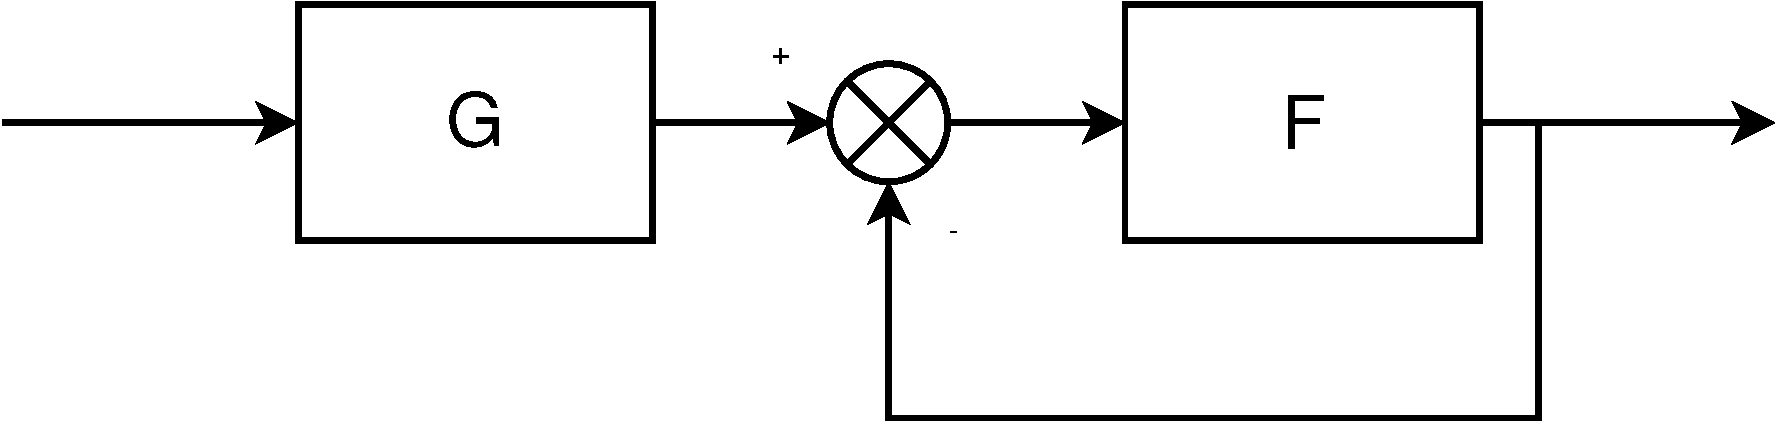
\includegraphics[width=8cm,
  keepaspectratio]{figuras/sistema1}



  \caption{\label{cap:DBloques}Diagrama de bloques del sistema
    ejemplo}
\end{figure}


Primero construiremos el bloque de la derecha, el más cercano a la
salida. Su función de transferencia es:
$DCHA(s)=\frac{10}{s^{2}(s+3)}$ de modo que empezaremos definiendo su
bloque básico:
\begin{verbatim}
>> DCHA=zp([],[0,0,-3],10,TSAM=0,'DCHAIN','DCHAOUT');
\end{verbatim} El paso siguiente es duplicar su salida 
\begin{verbatim}
>> DCHAdup=sysdup(DCHA,[],'DCHAIN');
DCHAdup =
{
  a =

    -3   1   0
     0   0   1
     0   0   0

  b =

    0  0
    0  0
    1  1

  c =

    10   0   0

  d =

    0  0

  inname =

  {
    [1,1] = DCHAIN
    [1,2] = DCHAIN(dup)
  }

  n = 3
  nz = 0
  outname =

  {
    [1,1] = DCHAOUT
  }

  stname =

  {
    [1,1] = x_1
    [1,2] = x_2
    [1,3] = x_3
  }

  sys =

    2  0  0  1

  tsam = 0
  yd = 0
}

\end{verbatim}
Como vemos ha aparecido una nueva entrada llamada
\texttt{DCHAIN(dup)}, copia de \texttt{DCHAIN}. Ahora ya podemos crear
la recirculación del primer estadio no sin antes cambiar el signo de
la nueva puerta de salida:
\begin{verbatim}
>> DCHAdup=sysscale(DCHAdup,[],diag([1,-1]));
\end{verbatim} 
Este es un modo abrevidado de utilizar la función \texttt{syscale},
consultando la ayuda aprenderemos a utilizarla de un modo más
intuitivo.  Ahora conectamos la señal a la salida con la nueva puerta
de entrada y finalmente simplificamos el sistema par que tenga una
única entrada.  Como paso final comprobaremos que el resultado es
realmente el deseado escribiendo la función de transferencia del
sistema.

\begin{verbatim}
>> DCHAend=sysconnect(DCHAdup,'DCHAOUT','DCHAIN(dup)');
>> DCHAend=sysprune(DCHAend,'DCHAOUT','DCHAIN');
>> sysout(DCHAend,'tf')
Input(s)
      1: DCHAIN

Output(s):
     1: DCHAOUT

transfer function form:
10
----------------------------------
1*s^3 + 3*s^2 + 1.554e-15*s^1 + 10
\end{verbatim} 

La definición del bloque de la izquierda es la única limitación del
OCTS. No puede definir bloques cuyo número de ceros sea mayor a su
número de polos. Esto es debido a la forma que tiene de hacer los
cálculos internos para crear la estructura de datos. Para seguir con
el ejemplo tendremos que romper la estructura de datos creada por el
primer bloque con recirculación, multiplicarla por el polinomio del
bloque de la izquierda y finalmente crear la última recirculación.
Esto no significa ningún problema porque podemos pasar de la
representación como estructura a función de transferencia sólo con
aplicar la función \texttt{sys2tf}
\begin{verbatim}
>> [num,den]=sys2tf(DCHAend);
\end{verbatim} 
Para multiplicar el numerador de la función de transferencia por el
nuevo término utilizamos la función \texttt{conv} que ya vimos en la
sección dedicada al cálculo con polinomios.
\begin{verbatim}
>> num=conv([1,2],num);
\end{verbatim} 
El paso siguiente es reconvertir la función de transferencia en el
tipo estructura.
\begin{verbatim}
>> TOTAL=tf(num,den,TSAM=0,'IN','OUT');
>> sysout(TOTAL,'tf')
Input(s)
      1: IN

Output(s):
     1: OUT

transfer function form:
10*s^1 + 20
----------------------------------
1*s^3 + 3*s^2 + 1.554e-15*s^1 + 10
\end{verbatim}


\subsection{Análisis en frecuencia}

\label{sec:analisis}

De nada servirían todas las funciones de construcción de bloques si
luego no podemos analizar el comportamiento de nuestro sistema. Esta
parte del toolkit es sin duda su punto fuerte.

Una de las pocas cosas que debemos tener en cuenta es que el sistema
que se estáresolviendo cuando se hace el análisis en frecuencias no
es el original sino el de la figura \ref{cap:DBloques2}:

%
\begin{figure}

 \centering{} 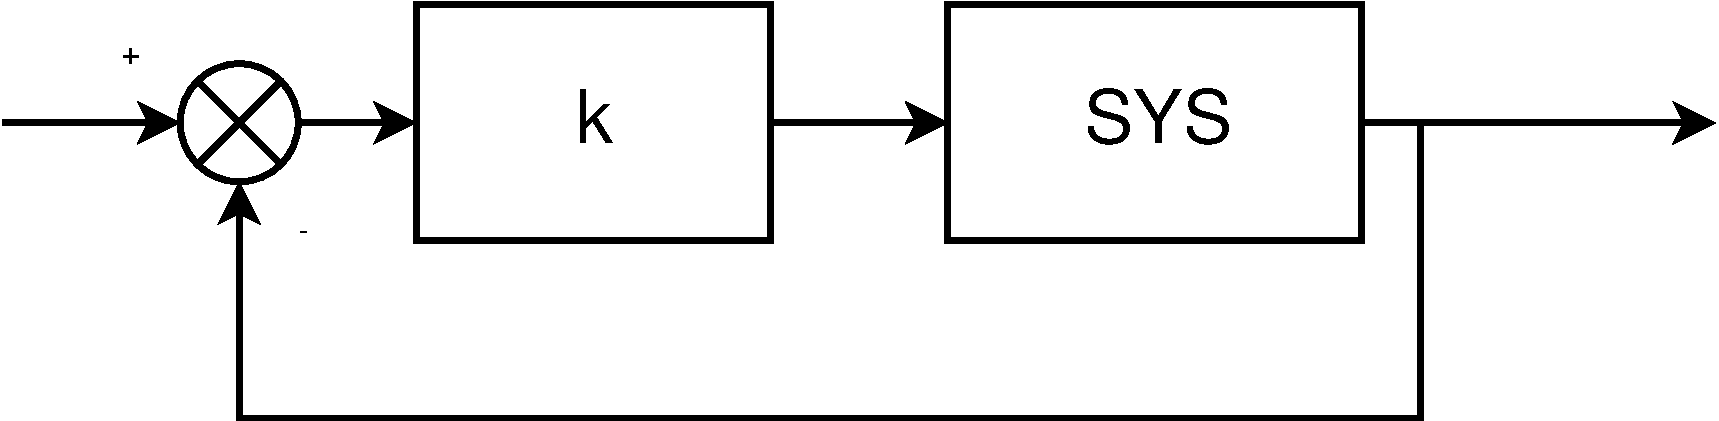
\includegraphics[width=8cm, keepaspectratio]{figuras/sistema2}


\caption{\label{cap:DBloques2}Diagrama de bloques resuelto}
\end{figure}


\begin{description}
\item [bode\index{bode}]Hace el análisis bode del sistema. En el caso
que no se soliciten argumentos de salida se dibuja el diagrama bode 
\item [nyquist\index{nyquist}]Hace el análisis nyquist de sistema. 
\item [nichols\index{nichols}]Hace en análisis nichols del sistema. 
\end{description}

\subsubsection{Ejemplo de análisis en frecuencia}

\label{sec:ejercicioanalisis} Aprovechando que ya hemos creado un
sistema en la sesión para hacer el diagrama de Nyquist basta con:
\begin{verbatim}
>> nyquist(TOTAL)
\end{verbatim} Lo que genera la figura (\ref{fig:nyquist}). %
\begin{figure}
 \centering
    \includegraphics[width=12cm, keepaspectratio]{figuras/nyquistplot}


\caption{\label{fig:nyquist}Diagrama de Nyquist del sistema}
\end{figure}


Los diagramas de bode son igualmente sencillos de conseguir (figura
\ref{cap:bode}): 
\begin{verbatim}
>> bode(TOTAL)
\end{verbatim}%
\begin{figure}
 \centering
    \includegraphics[width=12cm, keepaspectratio]{figuras/bodeplot}

\caption{\label{cap:bode}Gráfica bode del sistema}
\end{figure}




%extensiones
\chapter{Extender Octave con otros
  lenguajes.\label{sec:Extender-Octave-con}}

\emph{Gran parte de esta sección, sobre todo los ejemplos, se basa en
  el tutorial {}``Dal segno al Coda'' de Paul Thomas. Podeis
  encontrarlo en el Wiki del proyecto Octave.}

Octave está escrito en C++, además es el lenguaje desde el que es más
sencillo extenderlo. Ahora deberíamos preguntarnos cuándo queremos
extender Octave. Si Matlab es un lenguaje de programación completo
deberíamos ser capaces de programar cualquier cosa. El problema es que
programar cualquier cosa no se hace a cualquier precio, los bucles son
un ejemplo de ello. Imaginemos que tenemos un programa que va
demasiado lento, que casi todo el tiempo de proceso se debe a la
evaluación de una función miles de millones de veces y el coste de
implementarla en otro lenguaje no es demasiado grande. La solución a
nuestro problema será escribir la función en C++ o en Fortran y luego
hacer un interfaz para que Octave pueda entenderla.

Para hacerlo antes tendremos que asegurarnos que disponemos de las
cabeceras (headers) de Octave. No se encuentran en algunos paquetes y
puede ser que tengamos que instalarlos a parte. Preparar la
infraestructura es un poco complejo, también necesitaremos un
compilador en el entorno accesible por consola, preferentemente los de
la colección gcc (gcc, g++, g77 y gfortran).

Las cabeceras sirven tanto para escribir pequeñas funciones como para
crear interfaces completos a librerías escritas en C, C++ o Fortran.
\texttt{mkoctfile} es la herramienta básica del desarrollo de Octave,
todos los archivos terminados en \texttt{.oct} han sido creados con
dicha función. Algunas de las librerías utilizadas son FFTW para las
transformadas rápidas de Fourier, ODEPACK para resolver ecuaciones
diferenciales ordinarias, UMFPACK para las matrices sparse y ATLAS
para el cálculo matricial. Los respectivos interfaces son una gran
fuente de información de cómo adecuar Octave a nuestras necesidades.


\section{Una advertencia antes de empezar a programar.}

Es posible que cuando probemos alguno de los ejemplos que se expondrán
a continuación recibamos un \emph{segmentation fault} o un resultado
sin ninguna lógica en vez de lo esperado. Muchas veces los programas
no son compilar y listo, los programadores experimentados en C y C++
saben de lo que hablo. Otra de las ventajas de los lenguajes
interpretados es que el intérprete es un binario \emph{standalone}%
\footnote{Este término informático proveniente de la expresión
  \emph{to stand alone} es el adjetivo que recibe un programa que
  despues de ser compilado ya no tiene ninguna dependencia externa;
  puede tenerlas en tiempo de compilación pero no en tiempo de
  ejecución. En un sistema operativo tipo UNIX esto es imposible
  porque todo depende como mínimo de la librería estándar de C.%
}. Octave es un programa que depende de varias librerías
externas, glibc, atlas, readline... Todas estas librerías deben ser
compiladas previamente de tal modo que sean compatibles con el
intérprete de Octave. Es normal que alguna de las dependenicas se
construya con un compilador distinto al que se utilice para Octave.
Normalmente no tendremos ningún problema pero esto no implica que no
se produzcan jamás.

Un ejemplo de ellos es cuando intentamos añadir código externo a
Octave con el programa mkoctfile. Lo que estamos haciendo es compilar
un archivo escrito en C++ con el compilador del sistema que puede ser
distinto al que se utilizó para Octave. Es incluso probable que los
compiladores sean incompatibles como por ejemplo el GCC4 y el intel
C++ compiler. Debemos tener en cuenta que Octave es a partir de ahora
un verdadero entorno de desarrollo, único y monolítico. Si queremos
ponernos a jugar de verdad lo mejor será que compilemos nosotros
mismos Octave con el compilador del sistema. Si somos incapaces de
hacerlo instalaremos el compilador con el que se construyó nuestro
Octave así como las librerías propias de C y C++ sobre las que
funciona.

Si podemos tener problemas con los compiladores de C++ con los de
Fortran debemos prepararnos para sufrir de lo lindo. Octave se compila
con gcc3, sin soporte para Fortran 95. Si queremos utilizar código en
este dialecto tendremos que utilizar gcc4 pero entonces las versiones
de las librerías de C++ serán incompatibles. Disponemos de dos
opciones:

\begin{enumerate}
\item Seguir con gcc3, escribir código en Fortran 77 y compilar con
  g77.
\item Pasarnos a la rama inestable de Octave, compilarla con gcc4 y
  gfortran y rezar para que no rompa nada.
\end{enumerate}
Por suerte estos problemas desaparecerán cuando gcc4 se consolide.


\section{Extender Octave con C++}

Una vez tengamos toda la infraestructura preparada podemos acoplar
cualquier función escrita en C++ a Octave. La diferencia entre los
archivos \texttt{.oct} y los \texttt{.mex} de Matlab es que en este
caso contamos con cabeceras que nos permiten manipular directamente
los argumentos de Octave. El header principal es \texttt{oct.h}, en él
se encuentran las definiciones de todos los argumentos necesarios.

Empezaremos con el siguiente archivo de ejemplo que llamaremos
\texttt{eqlorentz.cc}:

\begin{verbatim}
#include <octave/oct.h>
DEFUN_DLD (eqlorentz,args, ,
    "Ecuacion de Lorentz en C++")
    {
    ColumnVector xdot (3);
    ColumnVector x (args(0).vector_value());
    int a=10;
    int b=28;
    double c=8./3;
    xdot(0) = a*(x(1)-x(0));
    xdot(1) = x(0)*(b-x(2))-x(1);
    xdot(2) = x(0)*x(1)-c*x(2);
    
    return octave_value (xdot);
    }
\end{verbatim}
Esta es la función de la ecuación diferencial del atractor de Lorentz:
$$
\begin{array}{l}
  \dot{x}=a(y-x)\\
  \dot{y}=x(b-z)-y\\
  \dot{z}=xy-cz\end{array}\qquad con\qquad 
a=10,\,\, b=28,\,\, c=\frac{8}{3}$$

Encontraremos el script que resuelve el problema en el ejercicio
\ref{sec:Ejercicio ode}.  Tenemos que evaluar la ecuación del atractor
un mínimo de 5000 veces, nos ahorraremos algo de tiempo escribiendo la
función en C++ y convirtiéndola en una función de Octave con:

\begin{verbatim}
bash ~/> mkoctfile eqlorentz.cc
\end{verbatim}

El resultado será un archivo llamado \texttt{eqlorentz.oct} que es
equivalente a cualquier archivo de función:

\begin{verbatim}
>> help eqlorentz
eqlorentz is the dynamically-linked function from the file
/home/guillem/sync/CursoScripting/ejercicios/eqlorentz.oct
Ecuacion de Lorentz en C++
>> eqlorentz([1,1,1],1)
ans =
    0.00000
   26.00000
   -1.66667
\end{verbatim}

Otra posibilidad interesante es la de crear subrutinas optimizadas
para un tipo determinado de hardware. No es lo mismo llamar a una
subrutina que funcionaría en cualquier PC que optimizarla para
utilizar todas las posibilidades de un Xeon o de un Opteron.
\texttt{mkoctfile} no es más que un interface a los compiladores de la
família gcc, podemos pasarle parámetros de compilación para conseguir
una optimización máxima.

\subsection{Llamar funciones desde C++}

A medida que nos introduzcamos en la programación de extensiones para
Octave es probable que tengamos la necesidad de tomar funciones como
argumentos.  Un posible ejemplo de ello sería una rutina de integración
de una EDO; sin la función es imposible integrar nada.

Llamar una función desde Octave no es difícil pero tampoco es trivial.
Disponemos del tipo \texttt{octave\_function} que contiene todos
los métodos necesarios, el problema (si es que lo es) es que debe
referirse al argumento como un puntero.  Un \texttt{octave\_function} va a ser
siempre un puntero a una función.  Lo demás es ser un poco congruente
con la definición hecha anteriormente; una función se llama
mediante el método \texttt{do\_multi\_index\_op} que recibe como argumentos
el número de variables de entrada y un \texttt{octave\_value\_list} con
los mismos.  La salida será también un \texttt{octave\_value\_list}.

Ya en octave, para pasar las funciones debemos utilizar un function
handle, una función anónima o la función \texttt{inline}, de otro modo
Octave no sabrá que uno de los argumentos es una función.  Para que
la propia rutina lo compruebe se utilizan los métodos 
\texttt{is\_function\_handle} y \texttt{is\_inline\_function}.

Para ilustrar todo lo anterior utilizaremos el siguiente ejemplo:

\begin{verbatim}
/*testfh.cc*/
# include <octave/oct.h>

DEFUN_DLD(testfh,args, ,
          "testing how C++ can call an octave function")
{
  octave_value_list tmp;
  octave_value_list inval;
  octave_function *input_fcn=0;
  if (args(0).is_function_handle() || args(0).is_inline_function())
    input_fcn = args(0).function_value();
  else
    {
      error("this is not a function handle nor an inline function");
      return octave_value(-1);
    }
  double x = args(1).double_value();
  inval.append(octave_value(x));
  tmp = input_fcn->do_multi_index_op(1,inval);
  return tmp;
}
\end{verbatim}

Esta función recibe un function handle o un inline y un escalar de doble
precisión. Retorna la función evaluada en el punto definido por el escalar.
Para compilarlo haremos:

\begin{verbatim}
bash~/> mkoctfile testfh.cc
\end{verbatim}

Ya dentro de Octave ensayaremos su funcionamiento:

\begin{verbatim}
>> testfh('sin',.123)
error: this is not a function handle nor an inline function
>> testfh(@sin,pi/2)
ans = 1
>> testfh(@(x) sin(x)*exp(x/2),pi/4)
ans = 1.0472
>> testfh(inline('sin(x)*exp(x/2)'),pi/4)
ans = 1.0472
\end{verbatim}

Como vemos es capaz de entender function handles, function handles y
funciones inline.  Esta capacidad abre significativamente el abanico
de posibilidades de octave.  Las funciones escritas en C++ ya no son
algo monolítico, es decir, una subrutina tonta que sólo es capaz de
recibir y devolver valores.  Ahora podemos interactuar con toda
la plataforma de octave, incluso con las funciones pasadas por
cabecera.

\section{Extender Octave con Fortran}

Fortran es el lenguaje de cálculo científico por excelencia. Se ha
abandonado paulatinamente durante los últimos años por el hecho de que
no había ningún compilador libre de Fortran 95. Este hueco ha sido
llenado por los compiladores G95 y gfortran%
\footnote{gfortran es un fork del proyecto G95 por desavenencias en el
  desarrollo con su creador. gfortran está dentro de gcc mientras que
  G95 es un proyecto a parte.%
}. Ahora cualquier desarrollador puede programar en Fortran sin
necesidad de aceptar licencias restrictivas sobre su código.

Evidentemente el lenguaje de extensión natural de Octave es C++ pero
disponemos de la cabecera \texttt{f77-fcn} para comunicarnos con
subrutinas escritas en Fortran. Siendo Fortran tan popular en el
ámbito científico es lógico que Octave le de un trato especial.
Desgraciadamente la capacidad de integración de Fortran en Octave es
bastante limitada debido sobre todo a las dificultades de comunicación
entre C y Fortran.  Otros lenguajes interpretados cumplen mucho mejor
la labor de comunicarse con sus primos compilados como Python, Java o
Ruby.


\subsection{¿Por qué Fortran?}

Las subrutinas escritas en Fortran no son más rápidas en Octave que
las escritas en C++ sin embargo Fortran tiene otras muchas ventajas.
Fortran es, además de un lenguaje para aplicaciones científicas por
excelencia, el único en el que el uso de memoria es puramente
matricial.  Cuando declaramos un array en Fortran 95 lo hacemos con
rango, no sólo con la cantidad de memoria necesaria. Fortran es
claramente mejor que cualquier otro lenguaje de programación cuando
hay que calcular con variables de gran tamaño. Cuando operamos con
vectores, matrices y tensores a la vez es muy fácil equivocarse en los
índices o {}``pisar'' fuera de la matriz. Fortran reserva memoria de
una manera estricta y no tolera un mal uso de ella.

Otro motivo de peso es la manera radicalmente distinta en la que
Fortran y C tratan los arrays.  Mientras en Fortran el uso de la
memoria está detrás del concepto de array, en C no es más que una
sucesión de posiciones de memoria contiguas.  Cuando uno aprende C sin
ser un experto en ordenadores el concepto de puntero se le hace
tremendamente antinatural; más aún si la experiencia previa es en
Fortran. C es un lenguaje especialmente pequeño, esa es su gran
ventaja; pero no por ello es más simple o genera menos sutilezas.
Veamos por ejemplo los dos programas siguientes en C++.  En ellos se
pretende llamar a la ecuación diferencial de Lorentz y sacar el
resultado por pantalla.

\begin{verbatim}
#include <iostream>
using namespace std;

void lorentz(double t,double *y,double *yp)
{
  const int a=10;
  const int b=28;
  const double c=8./3;
  yp[0]=a*(y[1]-y[0]);
  yp[1]=y[0]*(b-y[2])-y[1];
  yp[2]=y[0]*y[1]-c*y[2];
}

int main(int argc,char *argv[])
{
  double y[3];
  double yp[3];

  y[0]=1.;
  y[1]=1.;
  y[2]=1.;
  lorentz(1.,y,yp);
  int i;
  for (i=0;i<3;i++)
    {
      cout << yp[i] << '\n';
    }
  return 0;
}
\end{verbatim}

La salida por pantalla es la siguiente:
\begin{verbatim}
guillem@desktop:~$ ./a.out
0
26
-1.66667
\end{verbatim}

Que es precisamente el resultado de la ecuación diferencial. Llama la
atención el hecho que en la cabecera no hemos definido ningun array
sino punteros.  En la cabecera de la función las definiciones

\begin{verbatim}
*double
double[3]
double[]
\end{verbatim}
Son equivalentes.

Ahora pensamos que a lo mejor C++ es muy listo y que podemos
ahorrarnos el bucle para obtener el resultado.  Probamos lo siguiente:

\begin{verbatim}
#include <iostream>
using namespace std;

void lorentz(double t,double *y,double *yp)
{
  const int a=10;
  const int b=28;
  const double c=8./3;
  yp[0]=a*(y[1]-y[0]);
  yp[1]=y[0]*(b-y[2])-y[1];
  yp[2]=y[0]*y[1]-c*y[2];
}

int main(int argc,char *argv[])
{
  double y[3];
  double yp[3];

  y[0]=1.;
  y[1]=1.;
  y[2]=1.;
  lorentz(1.,y,yp);
  int i;
  cout << yp << '\n';
  
  return 0;
}
\end{verbatim}

Y al ejecutar el programa:
\begin{verbatim}
0xbfce1360
\end{verbatim}
El programa ha escupido una dirección de memoria.  Para un programador
experimentado en C esto resultará tan obvio como desconcertante para
el resto de los mortales.  La relación entre los arrays y los punteros
es de amor-odio.  Salpica cualquier programa escrito en C o en C++ y
puede llegar a ser una tortura cuando sólo nos interesan los arrays.
Fortran no sólo es más seguro sino que ayuda a programar con pocos
errores tanto en la implementación del algoritmo como en el uso de la
memoria.

Otra ventaja importante es que la biblioteca estándar de Fortran
contiene funciones orientadas al cálculo científico y que la mayoría
de las bibliotecas de cálculo numérico están pensadas para comunicarse
con Fortran y no con C o C++.


\subsection{La difícil comunicación entre C y Fortran}
\label{sec:comunica-c-fort}
Fortran y C son lenguajes diametralmente opuestos, sobretodo en el uso
de la memoria. Mientras C permite al usuario jugar con las direcciones
de memoria de un modo transparente, incluso accediendo explícitamente
a los registros; Fortran utiliza la memoria en sentido estricto y
dejando pocas libertades al usuario. La gran diferencia entre ambos es
sin duda las llamadas a funciones y subrutinas, C llama por valor y
Fortran por referencia. ¿Qué significa eso? No olvidemos que Matlab
está escrito en C y Octave en C++, ambos utilizan una infraestructura
equivalente a cualquier programa en C. Para entender bien qué es una
llamada por valor y una llamada por referencia es necesario que
entendamos qué es una dirección de memoria y qué es un puntero.

Los ordenadores tienen tres tipos de memoria: la memoria cache, la
memoria física y la memoria virtual. La más importante de ellas para
un programa es la memoria física y es en la que debemos pensar cuando
programamos. Entrar en más disquisiciones sobre arquitectura de
ordenadores ahora sería inútil. Los programas no son más que procesos
de gestión de memoria; es almacenar algo en un sitio y decir qué hay
que hacer con ello. Si queremos sumar 2 más 2 tendremos que almacenar
un 2 en una posición de memoria, un 2 en otra, pasarlas por un sumador
y luego almacenar el resultado. Los lenguajes de programación de alto
nivel permiten escribir programas sin tener que pensar en todas estas
sutilezas.

Cuando en un código asignamos una variable a un argumento:

\begin{verbatim}
a=2
\end{verbatim}

estamos haciendo dos cosas: primero reservamos el espacio en memoria
necesario para almacenar un 2 y luego le estamos asignando el nombre
de una variable. El nombre está sólidamente unido a la posición de
memoria. Ahora supongamos que queremos referirnos a la variable a.
Podemos hacerlo de dos maneras. La primera es llamar el contenido de
a, es decir, 2. La segunda es referirnos a la variable según la
posición de memoria que ocupa. Llamamos posición de memoria a el punto
de la memoria física en el que se encuentra \emph{realmente} contenida
la variable y se expresa mediante una \emph{dirección de memoria} que
suele ser una cadena de 8 caracteres.

Esto nos permite distinguir entre dos tipos esenciales de variables,
las que contienen un valor y las que apuntan a una determinada
dirección de memoria. Las primeras se llaman variables y las segundas
reciben el nombre de \emph{punteros}. Los programadores experimentados
en C y C++ dominan el concepto de puntero pero los que no lo hayan
oído en su vida lo entenderán mejor con este pequeño programa en C:

\begin{verbatim}
#include <stdio.h>
int a;
int *ptr;
int main(int argc, char *argv[])
{
  a=2;
  ptr =  &a;
  printf("a es %i \n",a);
  printf("la direccion de a es %p \n",ptr);
  printf("el puntero ptr contiene %i \n",*ptr);
  return 0;
}
\end{verbatim}

Primero declaramos una variable de tipo entero y luego un puntero del
mismo tipo, luego le asignamos a la variable el valor de 2 y el
puntero a la posición de memoria de la variable. Imprimimos en
pantalla el resultado para saber qué contiene cada una de ellas y el
resultado es el siguiente:

\begin{verbatim}
a es 2
la direccion de a es 0x403020
el puntero ptr contiene 2
\end{verbatim}

Una vez hemos entendido la diferencia entre una posición de memoria y
el valor que esta contiene daremos el siguiente paso. Supongamos que
acabamos de escribir una función o una subrutina. Esta unidad de
programa necesita argumentos adicionales para funcionar especificados
en su cabecera. Si la función no recibe los argumentos necesarios en
tiempo de ejecución recibiremos un error. Pero acabamos de ver que
para el ordenador es equivalente recibir un valor que la posición de
memoria del bloque que la contiene. En un programa parecido al
anterior definimos la una función suma:

\begin{verbatim}
#include <stdio.h>

int a,b;
int sum(int a,int b)
{ 
  int result;
  result=a+b;
  return result;
}

int main(int argc, char *argv[])
{
  a=2;
  b=3;
  int resultado=sum(a,b);
  printf("la suma de %i y %i es %i \n",a,b,resultado);
  return 0;

}
\end{verbatim}

¿Qué hace C para pasar los valores a la función? C pasa los argumentos
a las funciones por valor. Esto significa que las memoria utilizada
por la función y por el programa principal son independientes. Cuando
pasamos los argumentos a la función suma se copia su valor a las
variables locales sin tocar las globales; la función espera un valor,
no una dirección de memoria; espera un 2, no un 0x748361.

Fortran es diametralmente opuesto a C en este sentido. Todas las
variables de Fortran son en realidad punteros. Fortran no sabe de
valores reales, sólo está interesado en posiciones de memoria. La
identificación entre la memoria y la variable es absoluta. Vamos a
descifrar lo dicho hasta ahora mediante un programa ejemplo:

\begin{verbatim}
program test
integer :: a,b,c
a=2
b=3
call sum(a,b,c)
write(*,*) c
end program test


subroutine sum(arg1,arg2,resultado)
  integer, intent(in) :: arg1,arg2
  integer, intent(out) :: resultado
  resultado=arg1+arg2
end subroutine sum
\end{verbatim}

Cuando llamamos a la subrutina sum no estamos pasando los valores 2 y
3 sino que estamos identificando las posiciones de memoria. Le estamos
diciendo a la subrutina que su arg1 se encuentra en la posición de a y
arg2 en la de b. Por eso tenemos que declarar las variables en las
subrutinas con el atributo intent; estamos operando con las mismas
posiciones de memoria, si nos equivocamos no podemos volver atrás.
Esto se llama pasar los argumentos por \emph{referencia}. Este punto
de vista es mucho menos versatil pero evita el uso de más memoria de
la necesaria. Por eso Fortran es un lenguaje muy indicado para manejar
variables de gran tamaño.

Esto significa que programando en C tendremos que pasar punteros y no
variables a las funciones escritas en Fortran.


\subsection{Llamar una función de C desde Fortran o la manera más difícil de sumar 2+2}

Para entender mejor el significado de la llamada por referencia en
Fortran vamos a aprovechar que los archivos objeto creados con el GCC
son independientes del frontend utilizado.  La estrategia es la
siguiente, crearemos una función en C que sume la primera y la segunda
variable y retorne el resultado en la tercera.  El código es el
siguiente:
\begin{verbatim}
void c_function_(int *a,int *b,int *c)
{
  *c=*a+*b;
}
\end{verbatim}
Algunas observaciones importantes:
\begin{enumerate}
\item Las funciones del tipo \texttt{void} son equivalentes a las
  subrutinas en Fortran.
\item El nombre de la función va seguido de una barra baja (trailing
  underscore) para que el nombre de la subrutina generada sea
  compatible con Fortran.  Ignoro el por qué pero de otro modo no
  funciona.
\item Como la función espera una asignación de argumentos por
  referencia espera punteros a las variables.  En la función debemos
  ser consecuentes y utilizar el operador de retorno de referencia
  para hacer la operación.
\end{enumerate}
Compilamos la función con:
\begin{verbatim}
bash$~/> gcc -c c_function.c
\end{verbatim}

Sólo falta crear el programa que implemente la llamada.  Es el
siguente:
\begin{verbatim}
program fortran_c_call

  integer :: a,b,c

  a=2
  b=2

  call c_function(a,b,c)

  write(*,*) c
end program fortran_c_call
\end{verbatim}
Lo compilamos y lo ejecutamos:
\begin{verbatim}
bash$~/> gfortran fortran_c_call.f90 c_function.o
bash$~/> a.out
        4
\end{verbatim}
Esta operación es imposible si el código objeto generado es
incompatible. Por muy extraño que parezca este tipo de
interoperabilidad es típica de un sistema UNIX.  Aunque C y Fortran
puedan parecer a veces agua y aceite no debemos olvidar que los
compiladores de Fortran no son más que programas escritos en C.

\subsection{Punteros y arrays}

El tipo esencial de Fortran es el array. Un array es un bloque de
memoria que contiene elementos del mismo tipo. Definimos un array
siempre con el apellido de su tipo; hablamos de array de enteros,
array de reales de doble precisión... En las variantes de Fortran más
recientes los arrays tienen rango. Fortran no trata del mismo modo un
array de rango 2 que uno de rango 3, ordenará los elementos de un modo
distinto para optimizar la lectura y la escritura. Hemos dicho que
todas las variables son en realidad punteros; un array es un puntero
al primer elemento, una sentencia de reserva de la memoria necesaria y
una regla de lectura y escritura. Si intentamos leer un elemento fuera
de los límites del array Fortran nos dará un error en tiempo de
ejecución

C no tiene ningún método para definir arrays, C sólo sabe reservar
memoria. Si intentamos emular el comportamiento de Fortran debemos
tener mucha precaución. Por mucho que intentemos reservar la memoria
justa y no llamar ningún elemento que no exista dentro de la variable
el rango desaparece. Para C estas dos declaraciones:

\begin{verbatim}
array[15];
array[3][5];
\end{verbatim}
son equivalentes. Será muy importante utilizar las cabeceras de Octave
porque nos proporcionarán los tipos necesarios para utilizar
cómodamente matrices y arrays.


\subsection{Escritura de \emph{wrappers} para funciones en
  Fortran.}

Aunque este es un conveniente importante no se requieren grandes
conocimientos de C++ para escribir uno. Para escribir un wrapper a la
ecuación diferencial del atractor de Lorentz:

\begin{verbatim}
subroutine eqlorentzfsub(x,xdot)
  real(8),dimension(:),intent(in) :: x
  real(8),dimension(:),intent(out) :: xdot
  real(8) :: a=10d0,b=28d0
  real(8) :: c
  c=8d0/3d0
  xdot(1)= a*(x(2)-x(1))
  xdot(2)= x(1)*(b-x(3)-x(2))
  xdot(3)= x(1)*x(2)-c*x(3)
end subroutine eqlorentzfsub
\end{verbatim}
El wrapper correspondiente para esta función es el siguiente:

\begin{verbatim}
#include <octave/oct.h>
#include "f77-fcn.h"
extern "C" int F77_FUNC (eqlorentzfsub,
                           EQLORENTZFSUB)(double*,double*);
DEFUN_DLD(eqlorentzf,args, ,"xdot=eqlorentz(x)")
{
  octave_value_list retval;
  ColumnVector wargin(args(0).vector_value());
  ColumnVector wargout(3);
  F77_FUNC(eqlorentzfsub,EQLORENTZFSUB)(wargin.fortran_vec(),
                                        wargout.fortran_vec());
  retval.append(wargout);
  return retval;
}
\end{verbatim}
Hacemos siempre uso de los objetos propocionados por las cabeceras de
octave, para ello se supone que tenemos nociones de programación
orientada a objetos. El wrapper sirve únicamente para pasar las
variables de entrada y salida a punteros que Fortran sea capaz de
reconocer.  Las variables de entrada y salida de la función para
octave van a ser \texttt{x} y \texttt{xdot} y las someteremos siempre
a las mismas transformaciones hasta ser punteros:

\begin{enumerate}
\item Recogeremos la variable de entrada de la función que Octave
  dejará en la variable \texttt{args}. Si es un escalar podemos
  utilizar una variable propia de C, si queremos un vector o una
  matriz tendremos que utilizar un tipo propio de Octave. En el caso
  del wrapper anterior declaramos un \texttt{ColumnVector} llamado
  \texttt{wargin} inicializado con la variable \texttt{args(0)} en
  forma de vector.
\item Declararemos la variable de salida, en este caso otro
  \texttt{ColumnVector}, al que también asignaremos un puntero.
  También declararemos la variable de retorno de la función de Octave,
  siempre como \texttt{octave\_value\_list}.
\item Llamaremos la función previamente compilada en Fortran mediante
  \texttt{F77\_FUNC} a la que pasaremos como argumentos los punteros
  que hemos creado para ella, en nuestro caso \texttt{argin} y
  \texttt{argout}. Previamente y fuera de la función
  \texttt{DEFUN\_DLD} declararemos la función externa donde
  definiremos \textbf{todos los argumentos como punteros a las
    variables de entrada y salida}.
\item Pasaremos la variable de salida \texttt{wargout} a la variable
  \texttt{retval} de retorno de la función en Fortran.
\end{enumerate}
Una vez tengamos la función y el wrapper escritos compilaremos la
función en Fortran con \textbf{un compilador compatible con el que se
  ha compilado octave}. El wrapper llamará al código objeto que se
haya creado con el archivo de Fortran. Los comandos son los
siguientes:

  \begin{verbatim}
bash$~/> gfortran -c eqlorentzfsub.f

bash$~/> mkoctfile eqlorentzf.cc eqlorentzfsub.o
\end{verbatim}
Una vez realizado el proceso aparecerá un archivo llamado
\texttt{eqlorentzf.oct} que ya es una función que Octave es capaz de
entender. La llamaremos en Octave del modo usual:

\begin{verbatim}
>> eqlorentzf([1,2,3])
ans =
   10
   23
   -6
\end{verbatim}
La necesidad de que los dos compiladores sean compatibles es un gran
contratiempo. De momento Octave sólo se puede compilar con la versión
3 del compilador GCC que sólo es capaz de compilar código en Fortran
77. Si intentamos mezclar archivos compilados con gcc 4, que entiende
Fortran 95, y gcc 3 muy probablemente tendremos un Segmentation Fault.
De momento nos conformaremos con escribir código en Fortran 77, aunque
no por mucho tiempo. Sólo como ejemplo la misma función en Fortran 77
se escribiría como:

\begin{verbatim}
      subroutine eqlorentzfsub(x,xdot)
      real*8 x(*),xdot(*)
      real*8 a,b,c

      a=10d0
      b=28d0
      c=8d0/3d0

      xdot(1)= a*(x(2)-x(1))
      xdot(2)= x(1)*(b-x(3)-x(2))
      xdot(3)= x(1)*x(2)-c*x(3)

      end subroutine eqlorentzfsub
\end{verbatim}
Podemos escribir wrappers que sean capaces de retornar los mensajes de
error de la subrutina. Para ello es necesario que el wrapper llame a
la función \texttt{F77\_XFCN} en vez de \texttt{F77\_FUNC}. Por
ejemplo, un wrapper para la subrutina siguiente%
\footnote{La subrutina está escrita en Fortran 77. Aunque se considere
  una variante obsoleta de Fortran es necesario conocer sus
  particularidades porque es el lenguaje en el que están escritas la
  mayoría de las bibliotecas de funciones. Es por ello que Octave
  prefiere utilizar una nomenclatura orientada a Fortran 77. Esto no
  genera ningún problema porque el código objeto generado por los
  compiladores de Fortran 77 es compatible con los de Fortran 95.
  Wrappers más sofisticados como f2py ya incorporan una sintaxis
  parecida a Fortran 95.%
}:
\begin{verbatim}
      SUBROUTINE TNINE (IOPT, PARMOD, PS, X, Y, Z, BX, BY, BZ)
      INTEGER IOPT
      DOUBLE PRECISION PARMOD(10), PS, X, Y, Z, BX, BY, BZ    
C     Este es un ejemplo para probar un wrapper.
C     Asigna la suma de PARMOD a PS, y X, Y, Z a BX, BY, BZ
      INTEGER I
      PS = 0D0
      DO I=1, 10
         PS = PS + PARMOD (I)
      END DO
      BX = X
      BY = Y
      BZ = Z
      END
\end{verbatim}
sería:

\begin{verbatim}
#include <octave/oct.h>
#include "f77-fcn.h"
extern "C"
{
  int F77_FUNC (tnine, TNINE) (const int & IOPT, const double* PARMOD,
                               double & PS,
                               const double & X, const double & Y,
                               const double & Z,
                               double & BX, double & BY, double & BZ );
}
DEFUN_DLD (t96, args, ,
           "- Loadable Function: [PS, BX, BY, BZ] = t96 (PM, X, Y, Z) \n\
 \n\
Returns the sum of PM in PS and X, Y, and Z in BX, BY, and BZ.")
{
  octave_value_list retval;
  const int dummy_integer = 0;
  Matrix pm;
  const double x = args(1).double_value(), y = args(2).double_value(),
  z = args(3).double_value();
  double ps, bx, by, bz;
  pm = args(0).matrix_value ();
  F77_XFCN (tnine, TNINE,
           (dummy_integer, pm.fortran_vec(), ps, x, y, z, bx, by, bz) );
  if (f77_exception_encountered)
    {
      error ("unrecoverable error in t96");
      return retval;
    }
  retval(0) = octave_value (ps);
  retval(1) = octave_value (bx);
  retval(2) = octave_value (by);
  retval(3) = octave_value (bz);
  return retval;
}
\end{verbatim}
Para convertir el archivo y el wrapper en una función de Octave
introducimos en la consola:

\begin{verbatim}
bash $~/> mkoctfile t96.cc tnine.f
\end{verbatim}
Y ya podemos llamarla como cualquier otra función de la colección:

\begin{verbatim}
>> help t96
t96 is the dynamically-linked function from the file
/home/guillem/Desktop/sandbox/t96.oct
- Funcion: [PS, BX, BY, BZ] = t96 (PM, X, Y, Z)
Asigna la suma de PM a PS y  X, Y, Z a BX, BY, BZ.
>> [uno,dos,tres,cuatro]=t96(1:10,pi,e,4)
uno = 55
dos = 3.1416
tres = 2.7183
cuatro = 4
\end{verbatim}

Hemos declarado todas las variables de la subrutina, tanto las
internas como las externas, para que si se produce un error en la
parte escrita en Fortran Octave sea capaz de encontrarlo. El wrapper
se encarga de tomar los argumentos de entrada, convertirlos en algo
que Fortran sea capaz de entender y recoger el resultado.

Octave también soporta la definición de los tipos derivados de
Fortran.  Para la subrutina:

\begin{verbatim}
subroutine f95sub2(din,dout)
type              ::        mytype
  real*8          ::        mydouble
  integer*4       ::        myint
end type mytype
type (mytype)     ::        din , dout
dout%mydouble = din%mydouble ** float( din%myint )
dout%myint = din%myint * din%myint
end subroutine f95sub2
\end{verbatim}

Primero la compilaremos con

\begin{verbatim}
bash $ ~/> gfortran -c f95sub.f90
\end{verbatim}

Escribiremos el wrapper:
\begin{verbatim}
#include <octave/oct.h>
#include <octave/f77-fcn.h>
struct mystruct {
  double mydouble;
  int myint;
  };
extern "C" int F77_FUNC (f95sub,f95SUB) ( mystruct &, mystruct &); 
DEFUN_DLD (f95demo, args , ,"[w,z] = f95demo( x , y ) \
returns w  = x ^y and z = y * y for integer y") {
  octave_value_list retval;
  mystruct dinptr , doutptr;
  dinptr.mydouble = args(0).scalar_value();
  dinptr.myint = int( args(1).scalar_value() );
  F77_FUNC (f95sub,f95SUB) (dinptr,doutptr );
  retval.append( octave_value( doutptr.mydouble ) );
  retval.append( octave_value( double( doutptr.myint  ) ) );
  return retval;
}
\end{verbatim}
Y finalmente llamaremos a \texttt{mkoctfile}:
\begin{verbatim}
bash$~/>mkoctfile f95demo.cc f95sub.o
\end{verbatim}

\section{Extender C++ con Octave}

Octave es un proyecto de software libre con un diseño bastante
acertado.  Tanto es así que las librerías de extensón de Octave junto
con la capacidad de incrustar el intérprete en una aplicación hace que
Octave sea una biblioteca de lo más completa. Esto proporciona a
Octave una cualidad no tan esperada; \textbf{puede utilizarse como
  extensión natural de C++ para el cálculo científico}. La cabecera
oct.h proporciona todos los tipos necesaros para el cálculo numérico,
matrices, vectores fila y columna, operaciones matriciales y
vectoriales... ¡Incluso resolución de EDOs! Para abrir boca nada mejor
que un pequeño experimento con un programa de lo más simple:

\begin{verbatim}
/*testoctavestandalone.cc*/
#include <iostream>
#include <oct.h>
int main(void)
{
  std::cout << "Octave y c++ \n";
  Matrix a=identity_matrix(2,2);
  std::cout << a;
}
\end{verbatim}

Para compilarlo utilizaremos la aplicación \texttt{mkoctfile} como
viene siendo habitual pero con la opción \texttt{-{}-link-stand-alone}
para generar un ejecutable.

\begin{verbatim}
$ mkoctfile --link-stand-alone testoctavestandalone.cc -o test.exe
\end{verbatim}
Y lo ejecutaremos, en un entorno UNIX...

\begin{verbatim}
$ ./test.exe
Octave y c++
 1 0
 0 1
\end{verbatim}

La biblioteca en C++ de Octave es mucho más potente como demuestra el
siguiente ejemplo:

\begin{verbatim}
/*test2.cc*/
#include <iostream>
#include <oct.h>
int main(void)
{
  Matrix a=Matrix(2,2);
  ColumnVector b=ColumnVector(2);
  a(0,0)=2.;
  a(1,0)=5.;
  a(0,1)=-6.;
  a(1,1)=3.;
  b(0)=1.;
  b(1)=0.;
  std::cout << a.solve(b);
  return 0;
}
\end{verbatim}
donde resolvemos el siguiente sistema de ecuaciones:

$$
\left(\begin{array}{cc}
    2 & -6\\
    5 & 3\end{array}\right)x= \left(\begin{array}{c}
    1\\
    0\end{array}\right)$$


\begin{verbatim}
$ mkoctfile --link-stand-alone test2.cc -o test.exe
$ ./test.exe 
0.0833333 
-0.138889 
\end{verbatim}

\section{MEX  (+)}

Si Octave se extiende mediante archivos \texttt{oct} Matlab lo hace
mediante archivos \texttt{mex}. Los dos métodos de extensión son
completamente distintos pero Octave también soporta las extensiones de
Matlab.

De este modo Octave no consigue la compatibilidad a nivel de
intérprete sino que también algunas extensiones de Matlab compilarán
con la biblioteca de Octave sin ningún cambio. Parece entonces
justificado describir sin demasiada precisión las funciones
\texttt{mex}

\subsection{Un ejemplo que simplemente funciona.}

Para comprobar que realmente Octave consigue este grado de
compatibilidad basta con tomar uno de los ejemplos de archivo mex
dentro de la documentación del propio Matlab.  En él ya se intuyen las
características más importantes de la programación en C para
Matlab. Es el siguiente:

\begin{verbatim}
nclude <string.h>
#include "mex.h"

void mexFunction(int nlhs, mxArray *plhs[ ],int nrhs, const mxArray *prhs[ ])
{
int j;
double *output;
double data[] = {1.0, 2.1, 3.0};


/* Create the array */
plhs[0] = mxCreateDoubleMatrix(1,3,mxREAL);
output = mxGetPr(plhs[0]);


/* Populate the output */
memcpy(output, data, 3*sizeof(double));

}
\end{verbatim}

Es un programa muy sencillo.  No recibe ningún argumento y se limita a
copiar un array de tres elementos en el argumento de
salida. Para compilarla con Octave en la consola de sistema:

\begin{verbatim}
$> mex testmex.c
\end{verbatim}

o bien

\begin{verbatim}
$> mkoctfile --mex testmex.c
\end{verbatim}


Esto generará un archivo llamado \texttt{testmex.mex} que es
equivalente a un archivo \texttt{oct}.  Para probarlo, dentro del
intérprete:

\begin{verbatim}
>> testmex()
ans =

   1.0000   2.1000   3.0000
\end{verbatim}



%%Parte II, ejercicios

\part{Ejercicios}

%Ejercicios resueltos
\chapter{Ejercicios resueltos}

%%%%%%%%%%%%%%%%%%%%%%%%%%%%%%%%%%%%%%%%%%%%%%%%%%

\emph{Este capítulo se basa en los ejemplos. Se propondrán una serie
de ejercicios, se comentarán los algoritmos necesarios para resolverlos
y finalmente se dará la solución a cada uno de ellos. }


\section*{Metodología de programación}

Quizás el mayor punto fuerte de Matlab o Octave no es su sencillez o
su productividad sino la gran cantidad de funciones útiles que nos
proporcionan. El núcleo de Matlab son sólo unos pocos Mbytes, en
cambio la instalación completa ocupa tres CD-ROMs. Todo son funciones
y archivos cuya razón de ser es hacernos la vida mucho más fácil.

Esto genera una ley un poco paradójica: \textbf{cuanto menos
  programemos mejores serán nuestros scripts}. Uno puede pensar que el
código que escribe uno mismo es mejor, que si al intuitérprete le pasamos
todas las líneas que debe usar irá más rápido. Que si tenemos que
cargar más funciones en memoria haremos que la ejecución vaya más
lenta...  Es justo lo contrario. La mayoría de las funciones en
Octave, por ejemplo, son funciones escritas en C++ o en Fortran
compiladas de una manera especial para que Octave las interprete.
Significa que la velocidad de ejecución de estas subrutinas será mucho
más cercana a la velocidad de los programas binarios que a la del
intérprete.


\section{Ejercicio. Cálculo de un gradiente}

Un cálculo muy común con una muestra de datos bidimensional es
calcular una especie de gradiente numérico definido como:$$
grad(M)=\left(\begin{array}{c}
    \frac{M(i,j+1)-M(i,j-1)}{2}\\
    \frac{M(i+1,j)-M(i-1,j)}{2}\end{array}\right)=\left(\begin{array}{c}
    \delta_{x}^{\prime}(M)\\
    \delta_{y}^{\prime}(M)\end{array}\right)$$ Que genera una matriz
de menor tamaño al perder los extremos. Escribir la función que
devuelve el resultado en una variable tipo estructura:
\texttt{grad.x}=$\delta_{x}^{\prime}(M)$ y
\texttt{grad.y}=$\delta_{y}^{\prime}(M)$.


\subsection{Guía para la resolución del ejercicio}

Lo más complicado de este ejercicio es entender el enunciado. En el
fondo es exactamente el mismo cálculo que un gradiente numérico con
la diferencia de que en este caso no nos importa la distancia entre
los puntos. Lo más práctico para calcular la fórmula es construir
una submatriz por cada elemento de la ecuación en diferencias; para
calcular la submatriz es necesario saber que el último elemento de
cualquier matriz o vector se puede llamar \texttt{end}. Por ejemplo,
si nosotros queremos los elementos del quinto al último del vector
\texttt{u} pero no sabemos sus dimensiones, en vez de calcularlo lo
más práctico es hacer \texttt{>\,{}> u(5:end)}.


\subsection{Solución del ejercicio}

  \begin{verbatim}
function[grad]=mygradient(M)

    grad.x = 0.5*(M(:,3:end)-M(:,1:end-2));

    grad.y = 0.5*(M(3:end,:)-M(1:end-2,:));
 \end{verbatim}


\section{Ejercicio.  Diseño de una tobera}

Queremos diseñar una tobera convergente divergente. Para ello
impondremos que el radio de salida sea 10 veces mayor que el radio de
la garganta, y que la tobera se forma mediante dos parábolas, una con
eje en $y$ y otra con eje en $x$. Las condiciones serán que en el
punto de empalme de los dos arcos haya continuidad tanto de la función
como de la derivada primera. Las dos funciones a ajustar serán
entonces (con el problema
convenientemente adimensionalizado)\\
$$y^{-}=Px^2+0.1\qquad y^{+}=\sqrt{Ax+B}$$
Entonces tenemos el sistema de ecuaciones siguiente, donde $l$ es el
punto en $x$ donde se empalman los dos arcos:
$$2Pl=\frac{A}{2\sqrt{Al+B}}$$
$$Pl^2+0.1=\sqrt{Ax+B}$$
$$\sqrt{A+B}=1$$
Donde se demuestra que existe solución para $P$ aproximadamente
$0.9<P<1.2$.

\begin{enumerate}
\item Resolver el sistema de ecuaciones anterior y representar las
  soluciones de $P=0.9$, $P=1$ y $P=1.2$
\end{enumerate}

\subsection{Guía para la resolución del ejercicio}

Lo primero que debemos hacer es entender el enunciado, para ver más
claro lo que se pide, es bueno dibujar las dos curvas que se nos proponen,
para ello haremos;

\begin{verbatim}
octave:1> fplot('[x. ^2+0.1,sqrt(x)]',[0,1])
\end{verbatim}
Para resolver numéricamente sistemas de ecuaciones lineales usaremos
la función \texttt{fsolve}. Para saber cómo funciona teclearemos en
la línea de comandos: 

\begin{verbatim}
octave:2> help fsolve
\end{verbatim}

\subsection{Solución del ejercicio}

El script que nos resuelve el problema es el siguiente: 

\begin{verbatim}
function[f]=ttb(x)
    global Pi
    f(1)=x(1)/(2*sqrt(x(1)*x(3)+x(2)))-2*Pi*x(3);
    f(2)=Pi*x(3)**2+0.1-sqrt(x(1)*x(3)+x(2));
    f(3)=sqrt(x(1)+x(2))-1;
end   
  
function[f]=tobera(x,a,b,l,P)
    if x<l
      f=P*(x*x)+0.1;
    else
      f=sqrt(a*x+b);
    endif
end   
x0=[1 1 1];
P=[0.9 1 1.2];
hold on   
for i=1:3
  global Pi
  Pi=P(i);
  [res]=fsolve('ttb',x0);
  xcoord=linspace(0,1,100);   
  for j=1:100
    tob(j)=tobera(xcoord(j),res(1),res(2),res(3),P(i));
  end
  plot(xcoord,tob)
end   
   
hold off
\end{verbatim}

El resultado lo vemos en la figura \ref{cap:Resultado-del-script-53}.

%
\begin{figure}[H]
\centering{}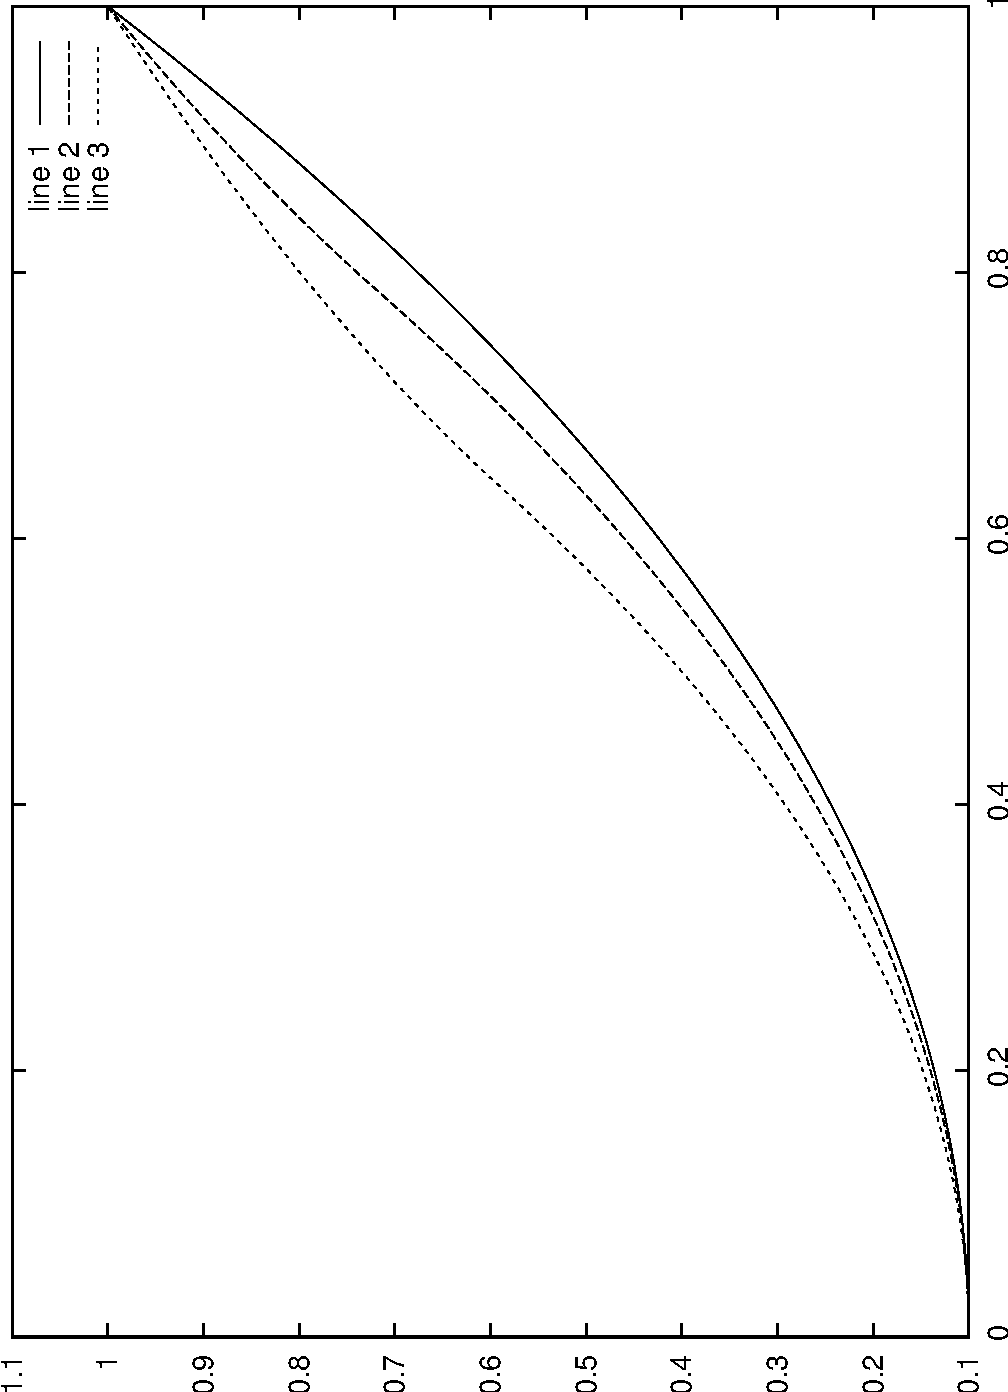
\includegraphics[%
  width=8cm,
  keepaspectratio,
  angle=-90]{figuras/figuraejercicio2}


\caption{\label{cap:Resultado-del-script-53}Resultado del script}
\end{figure}



\section{Ejercicio\label{sec:Ejercicio ode}.  El atractor de Lorentz}

Se quiere integrar la ecuación diferencial del \emph{Atractor de
  Lorentz}\index{Lorentz}, de ecuaciones:
$$
\begin{array}{l}
  \dot{x}=a(y-x)\\
  \dot{y}=x(b-z)-y\\
  \dot{z}=xy-cz\end{array}\qquad con\qquad a=10,\,\, b=28,\,\, c=\frac{8}{3}$$
y representarla en el espacio.


 \subsection{Guía para la resolución del Ejercicio}

 \begin{itemize}
 \item Primero escribimos la función correspondiente a la ecuación
   diferencial.  En las subrutinas de resolución de EDOs siempre
   tenemos que introducir la función de la forma
   $\frac{dx}{dt}=f(x,t)$ pudiendo ser cualquiera de las variables un
   vector.
 \item La rutina de Octave que nos integra la ecuación diferencial es
   \texttt{lsode}; en Matlab utilizaremos \texttt{ode45} porque el
   problema no es stiff.  Utilizar la ayuda para saber de qué manera
   tenemos que escribir la función de la ecuación diferencial.
 \item El comando para representar curvas paramétricas en 3
   dimensiones es \texttt{plot3}.
 \item Escribiremos todo en un script y lo ejecutaremos
 \end{itemize}

\subsection{Solución del ejercicio}


\subsubsection{Octave}

\begin{verbatim}
x=0;
function xdot=func(x,t)
a=10;b=28;c=8/3;
xdot(1,1)=a*(x(2)-x(1));
xdot(2,1)=x(1)*(b-x(3))-x(2);
xdot(3,1)=x(1)*x(2)-c*x(3);
end

x0=[1;1;1];
t=linspace(0,50,5000);
tic;x=lsode( "func ",x0,t);toc
plot3(x(:,1),x(:,2),x(:,3))
\end{verbatim}
dando como resultado la figura \ref{cap:Resultado-del-script-54}:

%
\begin{figure}[h]
\centering{}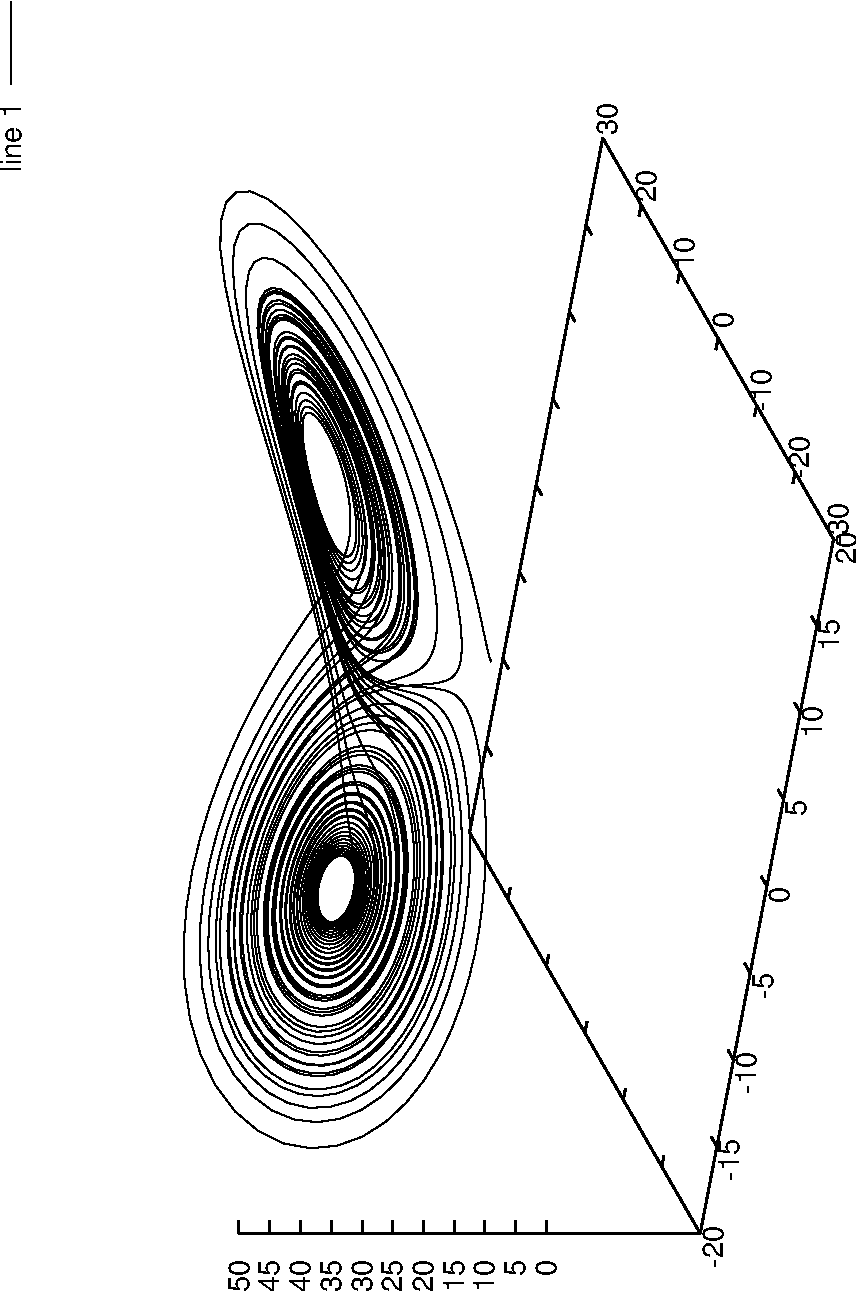
\includegraphics[%
  width=9cm,
  keepaspectratio,
  angle=-90]{figuras/figuraejercicio3}


\caption{\label{cap:Resultado-del-script-54}Resultado del script}
\end{figure}
 y el tiempo necesario para resolver la EDO que es de $3.1488$ segundos

La función \texttt{lsode} es mucho más versátil que las funciones
para la integración de ecuaciones diferenciales de Matlab. También
lo es en el sentido que es menos rigurosa en la manera de escribir
la función, en este caso hemos escrito la variable \texttt{xdot} en
forma de vector columna como nos obliga Matlab pero aceptaría igualmente
el uso de un vector columna.

Octave permite definir la función en el script de modo que podemos
resolver el problema con un único archivo.


\subsubsection{Octave no stiff}

El método de integración por defecto es explícito de modo que podemos
acelerar el proceso si utilizamos un esquema Adams-Bashforth incluyendo
este comando en el script:

\begin{verbatim}
lsode_options('integration method','non-stiff')
\end{verbatim}
Podemos hacerlo sin miedo porque el problema del atractor de Lorentz,
aunque es caótico, no es stiff. El tiempo de ejecución desciende a
$2.0016$ segundos.


\subsubsection{Octave y C++}

Ya hemos visto que podemos utilizar funciones escritas en otros
lenguajes para aumentar la velocidad de nuestros scripts. En el caso
de este ejercicio la velocidad conseguida por la función
\texttt{lsode} es aceptable pero podemos rebajarla bastante más
escribiendo la función de la ecuación diferencial en C++ y utilizando
la aplicación \texttt{mkoctfile}.  Ya hemos aprendido a hacerlo en la
sección \ref{sec:Extender-Octave-con}.  Supongamos que ya disponemos
del archivo \texttt{eqlorentz.oct} que usaremos del mismo modo que
cualquier función. El script que resuelve el problema es:

\begin{verbatim}
t=linspace(0,50,5000);
tic;x=lsode( "eqlorentz ",[1;1;1],t);toc
plot3(x(:,1),x(:,2),x(:,3))
\end{verbatim}

La nueva versión del script es capaz de resolver el problema en tan
sólo $0.28444$ segundos que es el 10\% del tiempo anterior.


\subsubsection{Octave y C++ no stiff}

La máxima optimización se consigue de este modo. El tiempo se rebaja
hasta $0.17314$ segundos. Aunque todas estas consideraciones sobre
velocidad pueden parecer inútiles debemos tener en cuenta que la
integración de EDOs y EDPs son los problemas numéricos más exigentes
en lo que respecta a uso de CPU. Entrar en este tipo de discusiones a
menudo comporta grandes beneficios aunque en este caso sean
irrisorios. Este último tiempo es comparable al obtenido con código
enteramente escrito en C++ y sólo un poco más lento que el escrito en
C o Fortran y el esfuerzo necesario para escribir el programa ha sido
mucho menor.%
\footnote{El uso de lenguajes {}``pegamento'' es una práctica cada día
  más habitual. Escribir un código enteramente en C o Fortran es
  bastante costoso tanto por el tiempo de desarrollo como por el
  esfuerzo necesario.  Muchas veces se empieza con un prototipo
  escrito con un lenguaje de RAD (Rapid Application Development) y
  posteriormente se reescriben sus partes.

  El mayor obstáculo en los proyectos grandes es que deben participar
  varios desarrolladores. Cada uno puede tener sus preferencias y las
  guías de estilo no siempre son una solución efectiva porque sólo
  arreglan el formato del código escrito. Todas estas dificultades
  unidas al aumento de velocidad de lenguajes como Python o Matlab ha
  llevado a la creación del concepto de {}``lenguaje pegamento''.

  Se trata de dejar a medias el código entre el prototipo y el
  programa definitivo. Partiendo del prototipo se van analizando las
  partes que consumen más recursos y, sin cambiar las cabeceras ni el
  esquema de variables, se reescriben en algún lenguaje rápido. Se
  para cuando se consigue un equilibrio entre nivel de interactividad,
  velocidad y coste de mantenimiento de código.

  Probablemente el mejor {}``lenguaje pegamento'' sea Python gracias a
  Pyrex, SWIG y F2Py. El primero es capaz de convertir el código
  Python en C++ automáticamente (rendimiento máximo y coste cero) y el
  segudo y el tercero son generadores automáticos de interfaces, SWIG
  para C y C++ y F2Py para Fortran 77 y Fortran 95.%
}


\subsubsection{Octave, C++ y Fortran}

Fortran es el lenguaje del cálculo matricial por excelencia. Hemos
visto ya la manera de producir wrappers para funciones en Fortran.
Su utilidad, más que para escribir pequeñas funciones donde el wrapper
puede ser más largo que el código útil, es la de acoplar subrutinas
que hagan uso de grandes cantidades de memoria con distintas precisiones
en coma flotante. La velocidad de Fortran es aproximadamente la misma
que la de C++ pero aporta ventajas distintas a la velocidad por lo
dicho anteriormente.


\subsubsection{Matlab}

En Matlab necesitaremos dos archivos. El archivo de función devuelve
el resultado en forma de vector columna (\texttt{lorentz.m}):

  \begin{verbatim}
function xdot=lorentz(t,x)
  a=10;b=28;c=8/3;
  xdot(1,1)=a*(x(2)-x(1));
  xdot(2,1)=x(1)*(b-x(3))-x(2);
  xdot(3,1)=x(1)*x(2)-c*x(3);
end
 \end{verbatim}
Fijémonos que el orden de las variables de la cabecera \texttt{x}
y \texttt{t} cambian según la rutina que usemos. El script será:

  \begin{verbatim}
x=0;t=0;
tic;[t,x]=ode45(@lorentz,[0,50],[1,1,1]);toc
plot3(x(:,1),x(:,2),x(:,3))
 \end{verbatim}

\section{Ejercicio.  Cálculo de una integral doble}

La integral
$$I=\int_{-\infty}^{\infty}\int_{-\infty}^{\infty}e^{-(x^{2}+y^{2})}dx\  dy$$
tiene como resultado $\pi$. Calcular la solución \textbf{con un único
comando}.


\subsection{Guía para la resolución del ejercicio}

La función que implementa la integral doble en matlab es \texttt{dblquad}
mientras que en Octave es \texttt{quad2dg}. Ambas funciones tienen
una cabecera idéntica, las únicas diferencias son el nombre y el algoritmo
de cálculo. Para pasarles la función a integrar como argumento usaremos
una sentencia \texttt{inline} o con una función anónima. Las rutinas
de integración tienen muchos problemas con las singularidades porque
trabajan con una precisión limitada, esto nos impide usar límites
de integración demasiado grandes y ni mucho menos podremos usar \texttt{Inf}
. Con $[-10,10]\times[-10,10]$ vamos a conseguir 5 cifras significativas.

Por si alguien aún no está trabajando con Octave esta es la ayuda
de la función \texttt{quad2dg}.

  \begin{verbatim}


>> help quad2dg
quad2dg is the user-defined function from the file
/usr/share/octave/2.1.64/site/m/octave-forge/integration/quad2dg.m   
usage:  int = quad2dg('Fun',xlow,xhigh,ylow,yhigh)
or
       int = quad2dg('Fun',xlow,xhigh,ylow,yhigh,tol)   
This function is similar to QUAD or QUAD8 for 2-dimensional integration,
but it uses a Gaussian quadrature integration scheme.
      int     -{}- value of the integral
      Fun     -{}- Fun(x,y) (function to be integrated)
      xlow    -{}- lower x limit of integration
      xhigh   -{}- upper x limit of integration
      ylow    -{}- lower y limit of integration
      yhigh   -{}- upper y limit of integration
      tol     -{}- tolerance parameter (optional)   
  
Note that if there are discontinuities the region of integration
should be broken up into separate pieces.  And if there are singularities,
a more appropriate integration quadrature should be used
(such as the Gauss-Chebyshev for a specific type of singularity).
 \end{verbatim}

\subsection{Solución del ejercicio}

Tenemos múltiples opciones:

\begin{itemize}
\item Con \texttt{inline}


  \begin{itemize}
  \item Matlab:\\
    \\
    \begin{minipage}[c]{1\textwidth}%

\begin{verbatim}
>> dblquad(inline('exp(-(x.*x+y.*y))'),-10,10,-10,10)

ans = 3.1416

\end{verbatim}
    \end{minipage}%

  \item Octave:\\
    \\
    \begin{minipage}[c]{1\textwidth}%

\begin{verbatim}
>> quad2dg(inline('exp(-(x.*x+y.*y))'),-10,10,-10,10)

ans = 3.1416

\end{verbatim}
    \end{minipage}%

  \end{itemize}
\item Con una función anónima:

  \begin{itemize}
  \item Matlab:\\
    \\
    \begin{minipage}[c]{1\linewidth}%

  \begin{verbatim}
>> dblquad(@(x,y) exp(-(x. ^2+y. ^2)),-10,10,-10,10)

ans = 3.1416

\end{verbatim}
\end{minipage}%

\item Octave:\\
\\
\begin{minipage}[c]{1\linewidth}% 

\begin{verbatim}
>> quad2dg(@(x,y) exp(-(x. ^2+y. ^2)),-10,10,-10,10)

ans = 3.1416

\end{verbatim}
\end{minipage}

\end{itemize}
\end{itemize}



\section{Ejercicio\label{sec:Ejercicio-Laplace}.  Resolución de la
  ecuación de Laplace en un dominio bidimensional}

Resolver la ecuación de Laplace en un dominio rectangular por
diferencias finitas con condiciones de contorno Dirichlet. La ecuación
de Laplace es la ecuación elíptica más sencilla: $\nabla^{2}\phi=0$,
que formulada en dos dimensiones se convierte en:\[
\frac{\partial^{2}\phi}{\partial
  x^{2}}+\frac{\partial^{2}\phi}{\partial y^{2}}=0\] Si se toman
diferencias finitas centradas de segundo orden para puntos dependiendo
de $i$ y $j$ llegamos a la ecuación en diferencias siguiente:

$$\frac{\phi(i+1,j)-2\phi(i,j)+\phi(i-1,)}{\Delta
  x^{2}}+\frac{\phi(i,j+1)-2\phi(i,j)+\phi(i,j-1)}{\Delta y^{2}}=0$$

Esta ecuación puede ser expresada en forma de sistema de ecuaciones
lineales $\mathbf{A}\varphi=b$, donde $b$ es un término independiente
que aparece al aplicar las condiciones de contorno y $\varphi$ es la
matriz de incógnitas $\phi$ expresada en forma de vector columna.  La
traslación del problema bidimensional a un vector de incógnitas es un
paso que nos puede costar de entender pero si tenemos una matriz de
incógnitas el tensor del sistema tendrá tres dimensiones con lo que ya
no tendremos rutinas escritas para resolver el sistema.

Usaremos como parámetros \texttt{dx=2}, \texttt{dy=3}, \texttt{n=50},
\texttt{m=50}. No podemos utilizar muchos más elementos porque se nos
quedaríamos sin memoria. Esta matriz de incógnitas se va a convertir
en un vector $n\times m$, lo que significa que la matriz del sistema
va a tener $(n\times m)^{2}$ elementos. Para un dominio de 100 por 100
puntos llegamos a $10^{8}$ puntos. Sería un buen caso de aplicación de
matrices sparse


\subsection{Guía para la resolución del ejercicio}

\begin{enumerate}
\item Escribir una función \texttt{place} que implemente la transformación
de la matriz al vector. La entrada serán los índices \texttt{i} y
\texttt{j} y el número de elementos por columna \texttt{n}. La salida
de la función será la posición en el vector posterior: \texttt{place=i+n(j-1)}.
\item Crear la matriz del sistema con la ecuación en diferencias y la función
creada en el apartado anterior
\item Poner las condiciones de contorno al gusto en el vector del término
independiente y resolver el sistema lineal

\begin{enumerate}
\item Para resolver el sistema lineal del modo usual basta con hacer
  \texttt{A\b}.
\item Para resolver el sistema con matrices sparse primero creamos la
  matriz
  sparse con:\\
  \texttt{spA=sparse(A)}~\\
  y luego resolveremos el sistema del modo usual. Es una buena idea
  eliminar la matriz del sistema de la memoria.
\end{enumerate}
\end{enumerate}

\subsection{Solución del ejercicio}

Primero definimos las constantes del problema

  \begin{verbatim}
dx=2;dy=3;n=50;m=25;
\end{verbatim}
A continuación creamos una función que reordena cualquier elemento de
una matriz bidimensional en un vector en el que se concatenan las
columnas.

  \begin{verbatim}
function place=place(i,j,n)

  place=i+n*(j-1);

end
\end{verbatim}
Ahora definimos la matriz del sistema teniendo en cuenta que la
incógnita no va a ser una matriz de dos dimensiones sino un vector.
Esto hace que la matriz del sistema tenga en realidad $nm\times nm$
elementos.

  \begin{verbatim}
A=zeros(n*m,n*m);
for i=1:n*m
  A(i,i)=1;
end
for i=2:n-1
  for j=2:m-1
    A(place(i,j,n),place(i,j,n))=-2*(1/(dx*dx)+1/(dy*dy));
    A(place(i,j,n),place(i-1,j,n))=1/(dx*dx);
    A(place(i,j,n),place(i+1,j,n))=1/(dx*dx);
    A(place(i,j,n),place(i,j-1,n))=1/(dy*dy);
    A(place(i,j,n),place(i,j+1,n))=1/(dy*dy);
  end
end
\end{verbatim}
Una vez definida la matriz del sistema creamos el vector del término
independiente que contiene las condiciones de contorno.

\begin{verbatim}
i=1;
for j=1:m
  b(place(i,j,n))=sin(pi*(j-1)/(m-1));
end
i=n;
for j=1:m
  b(place(i,j,n))=-sin(pi*(j-1)/(m-1));
end
j=1;
for i=1:n
  b(place(i,j,n))=sin(pi*(i-1)/(n-1));
end
j=n;
for i=1:n
  b(place(i,j,n))=0;
end
\end{verbatim}
Y finalmente resolvemos el sistema lineal.

\begin{verbatim}
T=A \b';
T=reshape(T,n,m);
contour(T);
\end{verbatim}
El resultado del script son las figuras
\ref{cap:Superficie-soluci=F3n} y \ref{cap:Contorno-solucion}.

%
\begin{figure}[H]
  \centering{}

  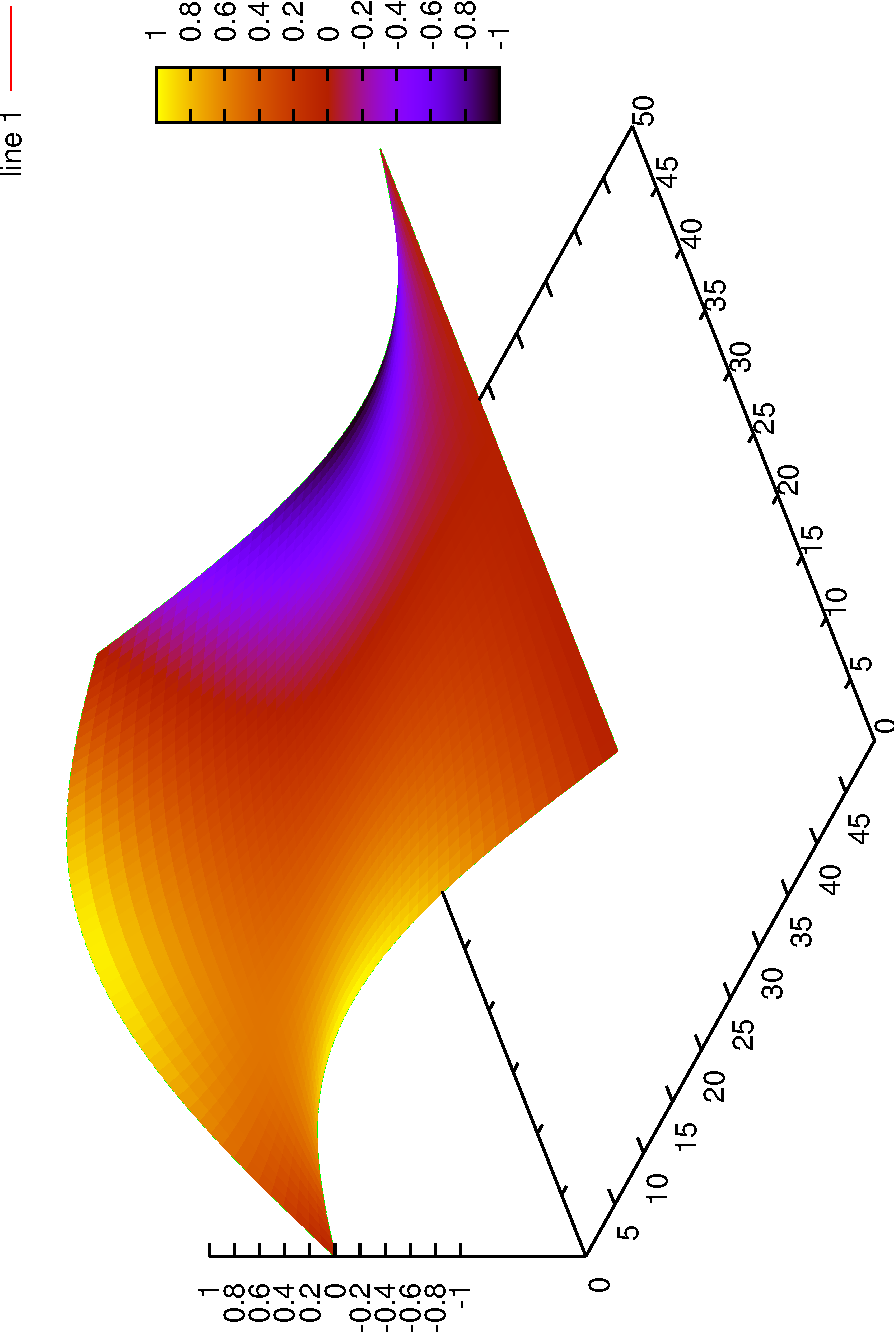
\includegraphics[%
  width=9cm,
  keepaspectratio,
  angle=-90]{figuras/mesh}


\caption{\label{cap:Superficie-soluci=F3n}Superficie solución}
\end{figure}


En el capítulo dedicado a la representación gráfica de soluciones
hemos hablado sobre lo poco útiles que suelen ser las superfícies
coloreadas para dar un resultado. Aunque una de estas representaciones
pueda parecer muy explicativa e intuitiva nunca debemos perder de
vista que lo que nos importa es mostrar un resultado y una superfície
no lo consigue. Por muy bien que coloquemos los colores o las barras
no conocemos el valor de cada punto con precisión y si encima colocamos
líneas de nivel dotamos al gráfico de un exceso de información.

Aunque sea mucho más espartano y pueda parecer inapropiado la solución
al problema son las curvas de nivel, en inglés \emph{contours} . Aunque
en un principio cueste un poco más entender la solución estamos ofreciendo
muchísima más información de un modo netamente más simple. Se podría
decir que no hay motivos para no utilizar las curvas de nivel a parte
de intentar demostrar nuestra pericia en el uso de Matlab.

%
\begin{figure}[H]
\centering{}

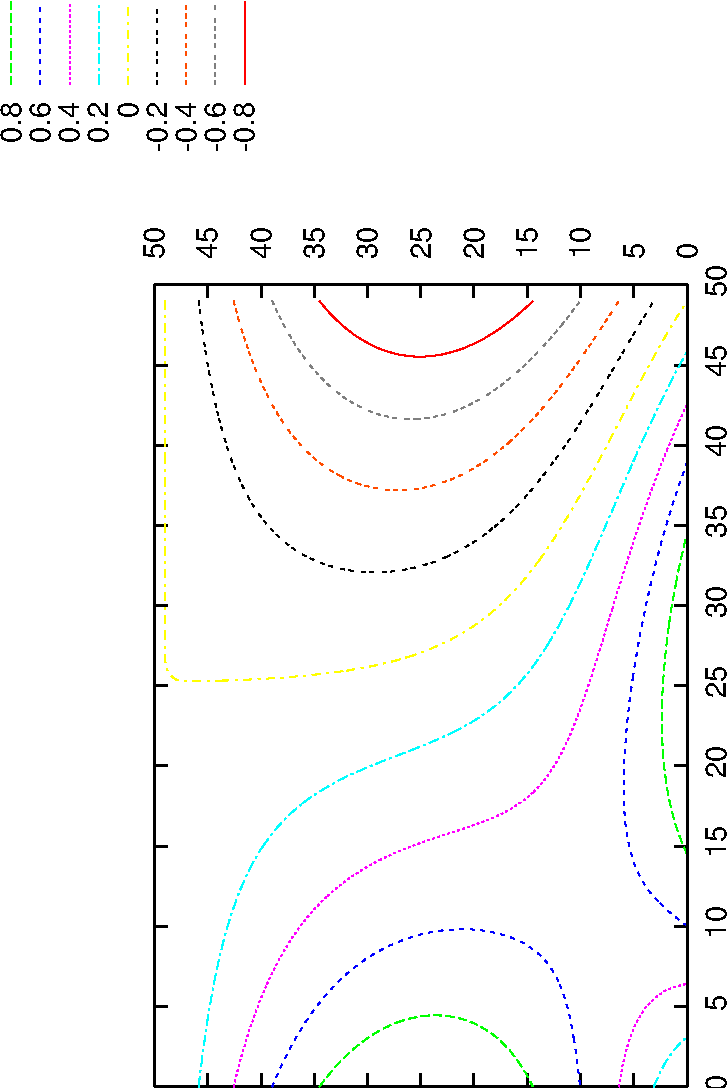
\includegraphics[%
  width=9cm,
  keepaspectratio,
  angle=-90]{figuras/contour}


\caption{\label{cap:Contorno-solucion}Superficie solución}
\end{figure}


Los gráficos de curvas de nivel pueden ajustarse perfectamente a nuestras
necesidades. Una práctica muy común y beneficiosa es la de embeber
el valor de cada curva dentro de la misma para no obligar al lector
a mirar la leyenda.


\subsubsection{Mejorar la solución. Cálculo de tiempos.}

Si analizamos el código de la solución es evidente que estamos
utilizando pocas funciones de la biblioteca. Además estamos haciendo
una de las pocas cosas casi prohibidas en Matlab que es crear una
matriz por fuerza bruta.

Un primer paso para mejorar la ejecución de un código es comprobar qué
partes consumen más recursos e intentar mejorarlas aisladamente.  Si
no somos capaces de conseguirlo nos replantearemos la solución de un
modo global. Para calcular los tiempos llenaremos el código con las
funciones \texttt{tic} y \texttt{toc}.

\begin{verbatim}
dx=2;
dy=3;
n=50;
m=50;
function place=place(i,j,n)
  place=i+n*(j-1);
end
A=zeros(n*m,n*m);
tic
for i=1:n*m
...
end
toc;disp('Creacion de la matriz del sistema'),disp(toc);tic;
i=1;
for j=1:m
  b(place(i,j,n))=sin(pi*(j-1)/(m-1));
...

  b(place(i,j,n))=0;
end
toc;disp('Creacion del vector b'),disp(toc);tic;
T=A \b';
toc;disp('Resolucion del sistema'),disp(toc);
T=reshape(T,n,m);
\end{verbatim}
Los tiempos en cada paso son:

\begin{verbatim}
>> ejercicio4
Creacion de la matriz del sistema
1.0611
Creacion del vector b
0.017038
Resolucion del sistema
2.1457
\end{verbatim}
Parece que debemos mejorar la construcción de la matriz del sistema y
la resolución del mismo. ¿Cómo? El primer paso suele ser analizar la
forma de la matriz con la función \texttt{spy}.

\begin{verbatim}
>> spy(A)
\end{verbatim}
Que tiene como resultado el siguiente patrón (figura
\ref{cap:Patr=F3n-de-elementos}):

%
\begin{figure}[h]
  \centering{}

  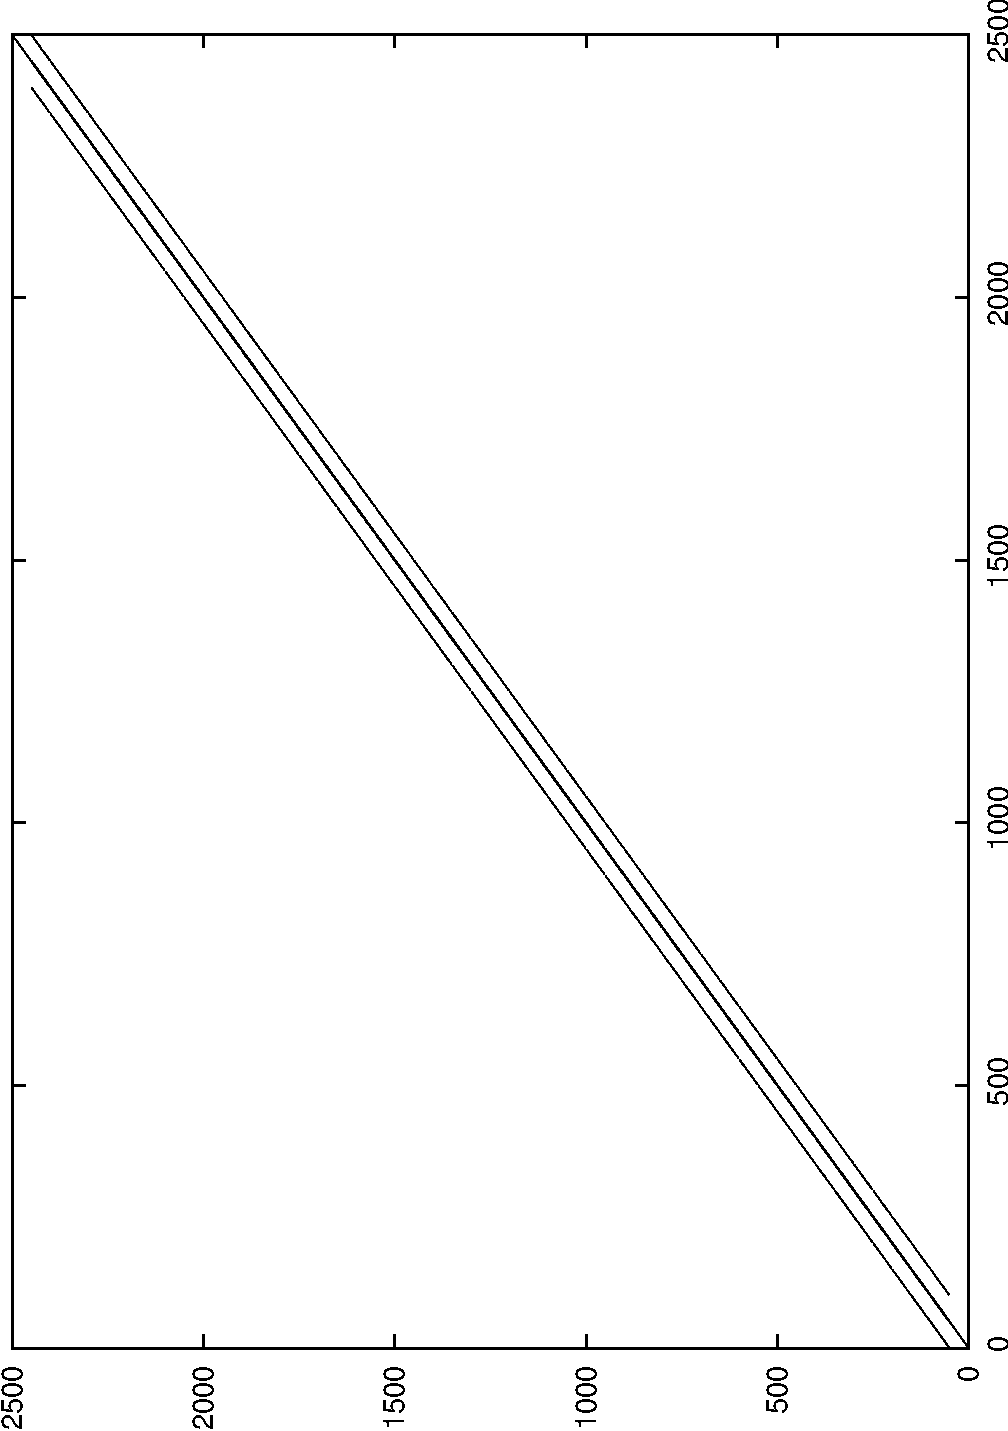
\includegraphics[%
  width=7cm,
  keepaspectratio,
  angle=-90]{figuras/spydiagonal}

  \caption{\label{cap:Patr=F3n-de-elementos}Patrón de elementos no
    nulos de la matriz del sistema}
\end{figure}


Esto nos demuestra que es una matriz n-diagonal por bandas lo que
entra en la definición de matriz sparse. Parece que la solución a
nuestros ligeros problemas de velocidad pueden solucionarse con el uso
de este tipo de matrices.


\subsubsection{Resolución del problema mediante matrices sparse(+)}

Uno de los errores cometidos en la primera solución propuesta es que
no utiliza las rutinas de creación de matrices disponibles. La
alternativa es utilizar bucles \texttt{for} para crearla por fuerza
bruta, solución de ningún modo recomendable. La mejor opción suele ser
utilizar la función \texttt{diag} pero como estamos tratando con
matrices sparse utilizaremos \texttt{spdiags}.


\subsubsection{Resolución del problema con un método iterativo.}

Para resolver el problema por un método directo es estrictamente
necesario romper la matriz para convertirla en un vector. Esto hace
que no podamos utilizar los operadores diferenciales en forma de
matriz tal como veremos en el ejercicio \ref{sec:Ejercicio-(Octave)}.
Un truco para mantener la integridad de la matriz y poder utilizar
estos operadores es resolver el problema con un método iterativo.
Aunque estemos multiplicando una matriz llena por matrices casi vacías
el resultado se acelera considerablemente.

La teoría de este método es bastante sencilla. Si aplicamos el
operador laplaciano a la matriz bidimensional el problema numérico se
reescribe del siguiente modo.$$
\mathbf{D_{x}}\phi+\phi\mathbf{D_{y}}^{\top}=0$$


Este planteamiento carece de solución analítica pero sirve para
plantear un problema iterativo en el que sólo hay que evaluar la
expresión.  Empezaremos la subrutina del mismo modo que la anterior,
definiendo la función que recoloca los elementos de la matriz
bidimensional.

\begin{verbatim}
dx=2;dy=3;global n=50;global m=50;
% resolucion del problema con un solver iterativo construccion de los
% operadores en diferencias
function place=place(i,j,n)
  place=i+n*(j-1);
end
\end{verbatim}
Ahora definiremos las matrices de los operadores diferenciales. Las
definimos como variables globales al igual que las dimensiones de la
matriz porque son necesarios dentro de la función que calcula el paso
de iteración y ésta puede tener sólo un argumento de entrada.

\begin{verbatim}
global DX=diag([1,-2/(dx*dx).*ones(1,n-2),1],0).+...
          diag([0,1/(dx*dx).*ones(1,n-2)],1).+...
          diag([1/(dx*dx).*ones(1,n-2),0],-1);
global DY=diag([1,-2/(dy*dy).*ones(1,n-2),1],0).+...
          diag([0,1/(dy*dy).*ones(1,n-2)],1).+...
          diag([1/(dy*dy).*ones(1,n-2),0],-1);
\end{verbatim}
A continuación la función que calcula el término en cada iteración.
Notemos el hecho de que el argumento que recibe la función debe ser un
vector por requerimientos de la rutina de resolución. Para calcular
sobre las matrices utilizamos la función \texttt{reshape}.

\begin{verbatim}
function [AT]=calcstuff(T)
  global n
  global m
  global DX
  global DY
  rT=reshape(T,n,m);
  AT=reshape((DX*rT)+(rT*DY'),n*m,1);
end
\end{verbatim}
Ahora es el turno del término independiente que se define gracias a la
función \texttt{place} definida anteriormente.

\begin{verbatim}
i=1;j=1;b=1;
for j=1:m
  b(place(i,j,n))=sin(pi*(j-1)/(m-1));
end
i=n;
for j=1:m
  b(place(i,j,n))=-sin(pi*(j-1)/(m-1));
end
j=1;
for i=1:n
  b(place(i,j,n))=sin(pi*(i-1)/(n-1));
end
j=n;
for i=1:n
  b(place(i,j,n))=0;
end
\end{verbatim}
Y finalmente resolvemos el sistema.

\begin{verbatim}
tic;T=pcg('calcstuff',b',tol=1e-6,maxit=100);
disp('Tiempo de calculo'),disp(toc)
\end{verbatim}
El método utilizado para resolver el problema es el del {}``Gradiente
Conjugado Precondicionado''. Para utilizarlo debemos tener en cuenta
que el número de iteraciones por defecto no es sufciente; lo
corregimos y lo situamos en 100. El tiempo de proceso ha pasado de más
de tres segundos a 0.24929%
\footnote{Este ejercicio se ha resuelto en un AMD Athlon 3000+.%
}. Este programa no sería posible sin el uso inteligente de las
variables globales tal como las hemos utilizado en otros ejemplos.


\section{\label{sec:Ejercicio-(Octave)}Ejercicio.  Un problema de
calor unidimensional}

\emph{Este ejercicio requiere la función} \texttt{\emph{trisolve}}
\emph{que está disponible en Octave. Matlab no tiene ninguna rutina
  para resolver directamente sistemas tridiagonales porque trata este
  tipo de matrices como sparse. Para resolver el mismo problema en
  Matlab utilizaremos la función} \texttt{\emph{spdiags}} \emph{para
  montar la matriz sparse y luego resolveremos el sistema de
  ecuaciones del modo usual.}

Este ejercicio es una pequeña demostración de hasta dónde puede llegar
el ahorro de código con Matlab. Se trata de resolver la ecuación del
calor unidimensional con condiciones de contorno Dirichlet. La
discretización espacial serán diferencias finitas de sevundo órden y
la temporal será un esquema Crank Nicholson. Tomaremos este esquema
porque permite usar saltos de tiempo más grandes, de hecho nos
permitirá llegar al resultado sin tener que calcular ninguna iteración
temporal. La solución propuesta tiene sólo unas pocas líneas.

Una solución tan breve requiere algo de preparación matemática de modo
que hay que estar muy atento al planteamiento analítico del problema.


\subsubsection*{Discretización de la ecuación completa}

La ecuación del calor unidimensional es la EDP parabólica más
sencilla:
$$\partial_{t}\phi=\partial_{xx}\phi$$
 Como cualquier EDP parabólica se
puede formular de la siguientes manera:
$$ \frac{d\phi}{dt}=F(x,t)$$ 
Si
utilizamos un esquema Crank Nicholson la discretización temporal será
de la forma:
$$ \frac{\phi^{n+1}-\phi^{n}}{\Delta
  t}=\frac{1}{2}\left(F^{n+1}+F^{n}\right)$$
 Discretizando también el
lado derecho de la ecuación con diferencias finitas de segundo orden
llegamos a la ecuación discretizada:$$ \phi_{i}^{n+1}-\frac{\Delta
  t}{2}\left(\frac{\phi_{i+1}^{n+1}-2\phi_{i}^{n+1}+\phi_{i-1}^{n+1}}{\Delta
    x^{2}}\right)=\phi_{i}^{n}+\frac{\Delta
  t}{2}\left(\frac{\phi_{n+1}^{n}-2\phi_{i}^{n}+\phi_{i-1}^{n}}{\Delta
    x^{2}}\right)$$



\subsubsection*{Formulación matricial del problema.}

La ecuación anterior puede escribirse del modo siguiente:\[
\phi^{n+1}-\frac{\Delta
  t}{2}\mathbf{A}\phi^{n+1}=\phi^{n}+\frac{\Delta
  t}{2}\mathbf{A}\phi^{n}\] Agrupando términos, diciendo que
$\mathbf{B}^{\pm}=\mathbf{I}\pm\frac{\Delta t}{2}\mathbf{A}$ y
utilizando un $\Delta x=1$ (en el fondo es sólo adimensionalizar):\[
\mathbf{B}^{-}\phi^{n+1}=\mathbf{B}^{+}\phi^{n}\] donde la matriz
$\mathbf{A}$ tiene la forma:\[ \mathbf{A}=\left(\begin{array}{cccccc}
    -2 & 1 & 0 & 0 & \cdots & 0\\
    1 & -2 & 1 & 0 &  & 0\\
    0 & 1 & -2 & 1 &  & 0\\
    \vdots &  &  & \ddots &  & \vdots\\
    0 &  & 0 & 1 & -2 & 1\\
    0 & \cdots & 0 & 0 & 1 & -2\end{array}\right)\]



\subsubsection*{Condiciones de contorno e iniciales.}

\begin{itemize}
\item Condiciones de contorno: $\phi=0$ en $x=0$ y $\phi=1$ en $x=10$ 
\item Condiciones iniciales: $\phi(x)=0$ en los puntos interiores.
\item Dar una solución al problema para cualquier tiempo inferior a $t=10$.
\end{itemize}

\subsection{Guía para la resolución del ejercicio}

La dificultad de la resolución de este problema radica en la correcta
situación de las condiciones de contorno en la matriz, el uso correcto
de las submatrices y entender el funcionamiento de \texttt{trisolve}.


\subsection{Solución del ejercicio (Octave)}

Parte del ejercicio es entender qué estamos haciendo para llegar a la
solución. Lo bueno de abreviar en la escritura es que además el código
resultante suele ser mucho más rápido.

\begin{verbatim}
phi=zeros(10,1); phi(10,1)=1;
dt=0.1;
for i=1:50 #Activate loop in case of precision leak
  phi(2:9)=(1-dt)*phi(2:9)+0.5*dt*phi(1:8)+0.5*dt*phi(3:10);
  phi=trisolve(-[0.5*dt*ones(8,1);0],[1;(1+dt)*ones(8,1);1],...
  -[0;0.5*dt*ones(8,1)],phi);
end
\end{verbatim}
De este modo llegamos al resultado del problema con una precisión
aceptable. La figura del perfil de temperaturas es:

%
\begin{figure}[H]
  \centering{} \includegraphics[width=14cm,
  keepaspectratio]{figuras/calor}

  \caption{\label{cap:figcalor}Figura solución}
\end{figure}



\subsection{Solución del ejercicio (Matlab)}

Aunque la resolución de sistemas tridiagonales es un clásico del
cálculo numérico Matlab no cuenta con ninguna función para ello. El
motivo es que decidieron incluir las matrices tridiagonales dentro de
las matrices sparse. Las matrices tridiagonales o con pocas bandas se
resuelven eficientemente mediante un método directo con lo que en este
caso Matlab tiene un error de diseño.

No tendría ningún sentido programarse una función que resolviera
sistemas tridiagonales en Matlab porque todas estas rutinas son en el
fondo interfaces a bibliotecas en Fortran y en C por motivos de
velocidad.

En este caso la dimensión de la matriz no justifica el uso del
almacenamiento sparse de modo que utilizaremos la función
\texttt{diag} para crear una matriz según sus diagonales:

\begin{verbatim}
phi=zeros(10,1); phi(10,1)=1; dt=0.1;
B=diag([1,(1+dt)*ones(1,8),1],0)+...
    diag(-[0.5*dt*ones(1,8),0],-1)+...
    diag(-[0,0.5*dt*ones(1,8)],1);
for i=1:50
  phi(2:9)=(1-dt)*phi(2:9)+0.5*dt*phi(1:8)+0.5*dt*phi(3:10);
  phi=B \phi;
end
\end{verbatim}

\subsection{Comprobación de la evolución temporal}

La siguiente modificación del programa permite comprobar la evolución
de los pasos temporales sacando por pantalla varios estados temporales
de la solución. Aunque el problema es estable para saltos temporales
muy grandes preferiremos acortarlo por motivos de precisión.
Representaremos la solución en los tiempos
$t=[0.1,1,2,5,10,20,50,100]$. Muy atentos al modo de definir la
condición lógica que indica cuándo pintar la curva:

\begin{verbatim}
phi=zeros(10,1); phi(10,1)=1;dt=0.1;
# times to output
tout=[0.1,1,2,5,10,20,50,100];
hold on
for i=1:500 
  phi(2:9)=(1-dt)*phi(2:9)+0.5*dt*phi(1:8)+0.5*dt*phi(3:10);
  phi=trisolve(-[0.5*dt*ones(8,1);0],[1;(1+dt)*ones(8,1);1],...
  -[0;0.5*dt*ones(8,1)],phi);
  if sum((dt*i)*ones(1,length(tout))==tout)==1
    plot(phi)
  end
end
hold off
title('Solucion de la ecuacion del calor unidimensional')
xlabel('Longitud (adimensional)')
ylabel('Temperatura (adimensional)')
legend({'0.1','1','2','5','10','20','50','100'},2)
\end{verbatim}
Llegamos finalmente a la siguiente gráfica:

%
\begin{figure}[H]
  \centering{} \includegraphics[width=14cm,
  keepaspectratio]{figuras/calorevol}


  \caption{Evolución del perfil de temperaturas}
\end{figure}



\section{Ejercicio.  Nociones de turbulencia}


%Ejercicios propuestos
%%%%%%%%%%%%%%%%%%%%%%%%%%%%%%%%%%%%%%%%%%%%%%%%%%

\chapter{Ejercicios propuestos}

%%%%%%%%%%%%%%%%%%%%%%%%%%%%%%%%%%%%%%%%%%%%%%%%%%

\section{Matrices}

\begin{enumerate}
\item Dado el vector $x=[3,1,5,7,9,2,6]$, intentar prever a mano el
  resultado de las siguientes operaciones elementales\@.

  \begin{enumerate}
  \item \texttt{x(3)}
  \item \texttt{x(1:7)}
  \item \texttt{x(1:end)}
  \item \texttt{x(1:end-1)}
  \item \texttt{x(6:-2:1)}
  \item \texttt{x({[}1,6,2,1,1{]})}
  \item \texttt{sum(x)}
  \end{enumerate}
\item Dada la matriz $A=[2,4,1;6,2,7;3,5,9],$ calcular:

  \begin{enumerate}
  \item El vector \texttt{x1} que es la primera fila de $A$.
  \item Asignar las 2 primeras filas de $A$ a un vector llamado
    \texttt{y}.
  \item Calcular la suma de los elementos de las columnas de $A$.
  \item Calcular la suma de los elementos de las filas de $A$.
  \item Calcular la desviación estándar de cada columna de $A$.
  \end{enumerate}
\item Dada la matriz:
$$A=\left(\begin{array}{cccc}
      2 & 7 & 9 & 7\\
      3 & 1 & 5 & 6\\
      8 & 1 & 2 & 5\\
      4 & 2 & 8 & 7\end{array}\right)$$


  \begin{enumerate}
  \item Asignar los elementos impares de la matriz $A$ a otra matriz
  \item Asignar los elementos pares de la matriz $A$ a otra matriz
  \item Calular la raíz cuadrada de cada elemento de la matriz $A$
  \end{enumerate}
\end{enumerate}

\section{Programación}

\begin{enumerate}
\item Dado el vector \texttt{x={[}3 15 9 2 -1 0 -12 9 6 1{]}} escribir
  los comandos que darán los siguientes resultados generalizadoz para
  cualquier vector posible, preferiblemente en un único comando:

  \begin{enumerate}
  \item Convertir los elementos múltiples de 3 del vector en 3.
  \item Multiplicar los valores impares de x por cinco.
  \item Asignar los valores de módulo mayor a 10 a otro vector.
  \item Convertir los elementos que son menores a la media en cero
  \item Convertir los elementos que son mayores a la media en la
    media.
  \end{enumerate}
\item Escribir una función cuyo resultado sea:
$$ y(x)\left\{
    \begin{array}{ccc}
      2 & \qquad & x<6\\
      x-4 & \qquad & 6\leq x\leq20\\
      36-x & \qquad & 20\leq x\leq36\end{array}\right.$$
 representarla
  gráficamente para ver que tiene forma triangular con \texttt{fplot}.
\item Calcular el número $\pi$ mediante la seguiente serie:
$$\frac{\pi^{2}-8}{16}=\sum_{n=1}^{\infty}\frac{1}{(2n-1)^{2}(2n+1)^{2}}$$
  ¿Cuántos términos son necesarios para llegar a una precisión de
  $1\times10^{12}$?  ¿Cuánta es la precisión de la suma de 100
  términos?
\item Podemos calcular una serie de Fibonacci mediante la siguiente
  relación recursiva:
$$ F_{n}=F_{n-1}+F_{n-2}$$
con $F_{0}=F_{1}=1$.
  Calcular los 10 primeros números de la serie de Fibonacci. La
  relación $\frac{F_{n}}{F_{n-1}}$ se va aproximando al número áureo
  $\varphi=\frac{1+\sqrt{5}}{2}$ a medida que $n$ aumenta. ¿En qué
  término de la serie de Fibonacci nos acercamos al número áureo con
  una precisión de $1\times10^{12}$?
\item Los polinomios de Legendre $P_{n}(x)$ se definen con la
  siguiente relación recurrente:
$$  (n+1)P_{n+1}(x)-(2n+1)P_{n}(x)+nP_{n-1}(x)=0$$ con $P_{0}(x)=1$,
  $P_{1}(x)=x$ y $P_{2}(x)=\frac{3x^{2}-1}{2}$.  Cacular los tres
  siguientes polinomios y representarlos gráficamente en el intervalo
  {[}-1,1{]}
\item Se plantea el siguiente algoritmo para calcular el número $\pi$.
  Primero iniciar las constantes: $a=1$, $b=\frac{1}{\sqrt{2}}$,
  $t=\frac{1}{4}$ y $x=1$. Repetir la siguiente secuencia de comandos
  hasta que llegamos
  a la precisión deseada:\\
  \texttt{y = a}~\\
  \texttt{a = (a+b)/2}~\\
  \texttt{b = sqrt(b{*}y)}~\\
  \texttt{t = t-x{*}(y-a)\textasciicircum{}2}~\\
  \texttt{x = 2{*}x}\\
  Por último se toman los valores de $a$, $b$, y $t$ para estimar
  $\pi$ con:\\
  \texttt{pi\_est = ((a+b)\textasciicircum{}2)/(4{*}t)}~\\
  ¿Cuántas iteraciones son necesarias para llegar a una precisión de
  $1\times10^{12}$?
\item Escribir un programa que pida por línea de comandos un entero
  ($n$)
  y luego calcule lo siguiente.\\
  1. Mientras el valor de $n$ sea mayor que 1, cambiar el entero por
  la mitad de su valor si el entero es par; si es impar cambiarlo por
  tres veces su valor mas 1.\\
  2. Repetir estas operaciones cíclicamente y obtener el número de
  iteraciones hasta que el algoritmo se para en 1. Por ejemplo, para
  $n=10$ la secuencia es 5, 16, 8, 4, 2 y 1; entonces el número de
  iteraciones
  han sido 6.\\
  3. Representar la longitud de las secuencias en función del entero
  de entrada de 2 a 30 e intentar descubrir un patrón. Si no se deduce
  intentarlo con más números.\\
  4. ¿Hay algún número para el que la secuencia sea interminable?
\item Escribir un programa que convierta números romanos en decimales.
  La
  tabla de conversion es: \\
  \begin{minipage}[c]{1\linewidth}%
\centering{}\begin{tabular}{|c|c|}
\hline 
Romanos&
Decimales\tabularnewline
\hline
\hline 
I&
1\tabularnewline
\hline 
V&
5\tabularnewline
\hline 
X&
10\tabularnewline
\hline 
L&
50\tabularnewline
\hline 
C&
100\tabularnewline
\hline 
D&
500\tabularnewline
\hline 
M&
1000\tabularnewline
\hline
\end{tabular}\end{minipage}%

\item Escribir un programa que haga la función inversa, que pase de números
decimales a romanos. En ambos casos el número se pedirá por pantalla.
\end{enumerate}

\section{Álgebra lineal}

\begin{enumerate}
\item Resolver el siguiente sistema de ecuaciones lineales:$$
  \begin{array}{ccccccc}
    x & - & 2y & + & 3z & = & 9\\
    -x & + & 3y &  &  & = & 4\\
    2x & - & 5y & + & 5z & = & 17\end{array}$$

\item Sean $B=\{(1,0,0),(0,1,0),(0,0,1)\}$ y
  $B^{\prime}=\{(1,1,0),(1,-1,0),(0,0,1)\}$ bases en $\mathbb{R}^{3}$,
  y sea $$ A=\left[\begin{array}{ccc}
      1 & 3 & 0\\
      3 & 1 & 0\\
      0 & 0 & -2\end{array}\right]$$ la matriz de la aplicación lineal
  $T:\mathbb{R}^{3}\rightarrow\mathbb{R}^{3}$ en la base $B$, base
  cartesiana ortogonal se pide:

  \begin{enumerate}
  \item La matriz de cambio de base $P$ de $B^{\prime}$ a $B$
  \item La matriz de camnio de base $P^{-1}$de $B$ a $B^{\prime}$
  \item La matriz $A^{\prime}$ que es la matriz $A$ expresada en la
    base $B^{\prime}$.
  \item Sea$$ [v]_{B^{\prime}}=\left[\begin{array}{c}
        1\\
        2\\
        3\end{array}\right]$$
 encontrar $[v]_{B}$ y $[T(v)]_{B}$
  \item Encontrar $[T(v)]_{B^{\prime}}$ de dos maneras, primero como
    $P^{-1}[T(v)]_{B}$ y luego como $A^{\prime}[v]_{B^{\prime}}$.
  \end{enumerate}
\item Crear la matriz de $5\times5$ $T$ tal que:
$$ T_{kl}=k-l$$ y
  calcular sus autovalores y autovectores
\item Un proceso para encriptar un mensaje secreto es usar cierta
  matriz cuadrada con elementos enteros y cuya inversa es también
  entera. Se asigna un número a cada letra (A=1, B=2... espacio=28) y
  se procede como sigue a continuación. Supongamos que la matriz es:
  $$A=\left(\begin{array}{ccccc}
      1 & 2 & -3 & 4 & 5\\
      -2 & -5 & 8 & -8 & 9\\
      1 & 2 & -2 & 7 & 9\\
      1 & 1 & 0 & 6 & 12\\
      2 & 4 & -6 & 8 & 11\end{array}\right)$$ y el mensaje que
  queremos enviar es {}``ALGEBRA LINEAL''. Para codificar el mensaje
  romperemos la cadena de números en vectores de cinco elementos y los
  codificaremos.

  \begin{enumerate}
  \item ¿Cuál será la cadena de datos encriptada que enviaremos?
  \item Descifrar el mensaje: 48 64 -40 300 472 61 96 -90 346 538 16
    -5 71 182 332 68 131 -176 322 411 66 125 -170 301 417.
  \end{enumerate}
\end{enumerate}

\section{Cálculo y Ecuaciones Diferenciales Ordinarias.}

\begin{enumerate}
\item Hallar el área $A$ de la región del plano comprendida entre la
  curva
$$ y=\frac{x^{2}-1}{x^{2}+1}$$
 y su asíntota. ($2\pi$)
\item Hallar la longitud $s$ del arco de cicloide
$$ \left\{
    \begin{array}{ccc}
      x & = & a(t-\sin t)\\
      y & = & a(t-\cos t)\end{array}\right.\quad0\leq t\leq2\pi$$
  ($8a$)
\item Hallar el centro de masas de la cardioide
$$
  \rho=a(1+\cos\theta)$$ (Sobre el eje de simetría y en
  $x=\frac{4a}{5}$)
\item El péndulo esférico tiene de ecuaciones:$$
  \ddot{\theta}=\frac{l\dot{\varphi}\sin\theta\cos\theta-g\sin\theta}{l}$$
  $$
  \ddot{\varphi}=\frac{-2\dot{\varphi}\dot{\theta}\cos\theta}{\sin\theta}$$
  Integrarlas con una condición inicial cualquiera y representar
  gráficamente las trayectorias.
\item Resolver el sistema de ecuaciones diferenciales siguiente:$$
  \begin{array}{ccc}
    \frac{dx}{dt} & = & ax+bxy-cx^{2}\\
    \frac{dy}{dt} & = & dxy-ey\end{array}$$
  donde $a=0.05$, $b=0.0002$, $c=0.00001$, $d=0.0003$ y $e=0.06$.
  Crear el mapa de fases linealizando la ecuación y utilizando el comando
  \texttt{quiver}. Resolverlo para $t\in[0,300]$ con distintos valores
  iniciales y ver que las soluciones siguen el camino marcado por el
  gradiente numérico.
\item Resolver el siguiente sistema que representa un modelo
  depredador-presa:$$
  \begin{array}{ccc}
    x_{1}^{\prime} & = & x_{1}(15-x_{2})\\
    x_{2}^{\prime} & = & x_{2}(-15+x_{1}-x_{2})\end{array}$$
  con condición inicial $x_{1}(0)=10$ y $x_{2}(0)=15$. Si los depredadores
  vienen dados por $x_{1}$, las presas por $x_{2}$ y el tiempo está
  medido en meses, ¿cuántos predadores y presas hay al cabo de un año?
  ¿Se extingue alguna de las especies en algún momento? Representar
  $x_{1}-x_{2}$ y $x_{1}$ en función de $x_{2}$.
\end{enumerate}

\section{Estadística y análisis de datos}

\begin{enumerate}
\item Generar una muestra de 1000 elementos que sigan una distribución
  normal de media $10$ y desviación típica $9$.
\item Generar una muestra de 1000 elementos que sigan una distribución
  uniforme de media cero y desviación típica $10$.
\item Calcular y representar los caminos de un grupo de partículas con
  movimiento aleatorio confinadas por un par de barreras $B^{+}$ y
  $B^{-}$ unidades del orígen que es desde donde salen las partículas.
  Un movimiento aleatorio se calcula mediante la fórmula;
$$ x_{j+1}=x_{j}+s$$ donde $s$ es el número obtenido de una
  distribución normal estandarizada de números aleatorios según la
  función \texttt{randn}. Por ejemplo, N movimientos de la partícula
  se calcularían con el fragmento de código
  siguiente:\\
  \texttt{x(1)=0;}~\\
  \texttt{for j = 1:N}~\\
  \texttt{x(j+1) = x(j) + randn(1,1);}~\\
  \texttt{end}~\\
  Se cambiarán las condiciones de contorno de la siguiente manera:\\
  1. Reflexión. Cuando una partícula se encuentre fuera de la frontera
  se devolverá al interior del dominio como si hubiera rebotado en una
  pared\\
  2. Absorción. La partícula muere cuando entra en contacto con la pared.\\
  3. Absorción parcial. Es la combinación de los dos casos previos.
  La partícula rebota en la pared y la perfección de la colisión
  depende
  de una determinada distribución de probabilidad.\\
  Calcular una serie relevante de trayectorias y calcular:

  \begin{enumerate}
  \item La posición media de las partículas en función del tiempo.
  \item La desviación típica de las posiciones de las partículas en
    función del tiempo.
  \item ¿Influyen las condiciones de contorno en las distribuciones?
  \item Para los casos de absorción y absorción parcial representar
    gráficamente el número de partículas supervivientes en función del
    número de saltos temporales.
  \end{enumerate}
\item Desarrollar en serie de Fourier la función
  $f(x)=x^{2}\qquad-\pi<x<\pi$.
\end{enumerate}

\section{Control automático}

\begin{enumerate}
\item Determinar la respuesta a un impulso y a un escalón del sistema expresado
mediante la función discreta siguiente:$$
y(n)=x(n)-2\cos(\pi/8)y(n-1)+y(n-2)$$

\end{enumerate}


\appendix

\part{Apéndices}
%Los diez mandamientos de la programación en Matlab



%%%%%%%%%%%%%%%%%%%%%%%%%%%%%%%%%%%%%%%%%%%%%%%%%%
\chapter{Guía de estilo. Los 10 mandamientos}

%%%%%%%%%%%%%%%%%%%%%%%%%%%%%%%%%%%%%%%%%%%%%%%%%%

En muy bueno para un lenguaje de programación que tenga una guía de
estilo asociada. Cómo formatear el código debe ser algo más que una
marca de estilo personal, un estándar que todo el mundo siga a
rajatabla.

En algunos lenguajes la sintaxis viene acoplada a unas ciertas reglas
de escritura, por ejemplo Python nos obliga a tabular las estructuras;
si no ordenamos bien el inicio de las líneas el código no funcionará.
C, C++ y Java usan corchetes para agrupar niveles de ejecución y se
recomienda dejar sólo el corchete en la línea y tabular todo lo que
contenga.

En muchos casos estas reglas son en realidad recomendaciones. En
Fortran recomiendan marcar los niveles de ejecución con tabulados de
dos espacios, algo parecido se recomienda en Matlab. Pero tanto en
Fortran como en Matlab estas normas son sistemáticamente ignoradas. El
programador \emph{científico} no ha recibido ninguna educación sobre
las reglas de escritura y tiene muy poca experiencia con lenguajes más
fuertemente estructurados como C o Java. El resultado es un código
plano, desestructurado, desorganizado y mal comentado.

Una de las herramientas esenciales para evitar este desastre es el
editor de texto. Sería muy largo describir el funcionamiento de un
editor de texto, simplemente diremos que es un programa que edita
código fuente y que tiene todas las herramientas disponibles para que
sea mucho más fácil. Colorea las palabras clave, tabula el código
automáticamente, corrije algunos fallos comunes... Matlab posee un
buen editor de textos, pero no le llega ni a la suela del zapato a
Emacs o VIM. El funcionamiento de Emacs puede resultar hasta
sorprendente.  Imaginemos que abrimos un archivo de código escrito en
Fortran 95.  Está lleno de \texttt{if} y \texttt{do} sin ordenar y mal
tabulado.  Además el compilador nos dice que hay una estructura que
está sin cerrar; que nos falta un \texttt{end}. Si estamos editando el
archivo con Emacs sólo tenemos que pulsar \texttt{<Alt><Control><Q>} y
todo el texto se tabula automáticamente.

Sin embargo el estilo de un buen programador es insustituible. Matlab
no tiene ninguna guía de estilo, sin embargo puede decirse que existen
una serie de normas no escritas para que el código sea más leíble y,
no menos importante, ejecute rápido.

Estas normas parecen inservibles para pequeños scripts que escribimos
para consumo propio. He aprendido que cuando se recupera un script que
se ha escrito seis meses antes es como si lo hubiera escrito otro.
Siempre que escribamos un programa tomaremos esta actitud; lo estamos
escribiendo para que un desconocido lo entienda.

Todas las buenas prácticas se resumen en diez técnicas, los 10
mandamientos del Matlab.

\begin{description}
\item [1.]Utilizar funciones \texttt{inline} y \texttt{@} siempre que
  se pueda.
\end{description}
Ya hemos visto que en Matlab (que no en Octave) definir una nueva
función significa crear un archivo. Esto hace que el código de el
programa principal sea más difícil de entender y de comentar. Aunque
Matlab escala bien no es muy recomendable escribir programas demasiado
largos y si tenemos demasiadas funciones y archivos es que no estamos
haciendo las cosas bien.

Las sentencias \texttt{inline} y los \emph{function handles} nos
ayudan a mantener el código compacto y leíble.

\begin{description}
\item [2.]Usar bucles \texttt{for} sólo donde sea indispensable
\end{description}
Esta es la gran diferencia entre Matlab y Fortran. Una de las grandes
decepciones de los programadores en Fortran cuando utilizan Matlab es
la gran diferencia de velocidad. Esta diferencia existe y es de entre
uno y dos órdenes de magnitud. El problema es que es gravemente
acentuada por usar el estilo de Fortran en el código Matlab. En
Fortran los bucles \texttt{do} son endiabladamente rápidos. Cuando se
compila el código los contadores se optimizan como estructura entera,
incluso algunos compiladores advierten cuando los bucles encapsulados
no son dependientes y paralelizan la tarea automáticamente. El
programador en Fortran encapsula porque sabe que el compilador le va a
ayudar.

Matlab no es capaz de optimizar el código de esta manera porque su
arquitectura no lo permite. La solución para obtener una velocidad
aceptable es usar siempre submatrices.

\begin{description}
\item [3.]Usar estructuras \texttt{if} planas.
\end{description}
Cuando hablamos de condicionales dijimos que el encapsulado tipo
\emph{matroska} no era recomendable porque complica mucho la lectura
del código. Además disminuye la velocidad de ejecución por la creación
de más variables adicionales. Si utilizamos condiciones lógicas
compuestas (siempre dentro de un límite) el resultado será más leíble
y posiblemente más rápido.

\begin{description}
\item [4.]Utilizar las funciones de creación de matrices.
\end{description}
Las funciones como \texttt{zeros}, \texttt{ones}, \texttt{eye},
\texttt{linspace} o \texttt{meshgrid} son tremendamente útiles. El
código de un buen programador estará siempre lleno de composición de
estas funciones para generar matrices. La alternativa es utilizar
bucles, prohibido por el segundo mandamiento.

\begin{description}
\item [5.]Definir las variables de las cabeceras \emph{in situ}.
\end{description}
Cuando se pasan los argumentos a una función lo habitual es crear
primero las variables que los contienen y luego poner las variables en
la cabecera. Si lo hacemos es casi obligado hacerlo justo antes de
llamar a la función. De otro modo tendremos que navegar por el código
hasta encontrar dónde se define la variable que pasa el argumento.

Es recomendable también que las constantes o los argumentos simples se
definan directamente en la cabecera. Puede parecer que el resultado es
difícil de leer, pero cuando uno se acostumbra resulta ser todo lo
contrario. Es mucho mejor una línea con varios comandos que no
repartir sentencias asociadas por todo el código.

\begin{description}
\item [6.]Utilizar submatrices siempre que se pueda.
\end{description}
Este es el \emph{No matarás} de los mandamientos de Matlab. La
alternativa es utilizar bucles con un puntero que vaya rastreando la
matriz; demasiado lento. El equivalente de esta recomendación en
Fortran sería utilizar el \texttt{forall} en vez de los bucles
simples.

Esta práctica sólo tiene ventajas. El código es más leíble, es plano,
mejor encapsulado, se entiende perfectamente y es más rápido. Cuando
se dice que Matlab es un programa de cálculo matricial no se dice
gratuitamente. No hay que pensar contando índices con la notación del
sumatorio como en Fortran, hay que pensar matricialmente.

\begin{description}
\item [7.]Tabular bien los bloques de ejecución
\end{description}
Aunque ya hemos aprendido que lo más importante es evitar el
encapsulado de estructuras de ejecución en algunos casos no tendremos
más salida.  En ese caso el tabulado de cada uno de los bloques es muy
recomendable.  Además de obteber un resultado más leíble evitaremos
los errores tontos como los bucles o los condicionales sin cerrar.

\begin{description}
\item [8.]Comentar cualquier operación que lo precise.
\end{description}
Lo repito, cuando recuperemos código escrito unos meses antes será
como si lo hubiera escrito otro. puede ser que una sentencia
especialmente brillante sea además críptica; comentaremos
sistemáticamente todo lo que sea necesario.

\begin{description}
\item [9.]Escribir una cabecera de ayuda en cada función.
\end{description}
Este mandamiento es directamente derivado del octavo. A medida que
escribamos funciones terminaremos con una pequeña biblioteca personal.
El resultado será que tendremos que usar funciones sin recordar ni la
forma de su cabecera. El comando \texttt{help} es imprescindible no
sólo para las funciones de la biblioteca; también nos servirá en las
que escribamos nosotros mismos.

\begin{description}
\item [10.]Usar Octave en vez de Matlab y colaborar en el proyecto.
\end{description}
Las soluciones más justas no siempre son las más fáciles. Octave es
más espartano y difícil pero ha sido posible gracias al esfuerzo de
muchos desarrolladores que han colaborado desinteresadamente en el
proyecto. El resultado es un programa de gran calidad que no para de
mejorar día a día.

El hecho de que se trate de software libre es un valor añadido.
Podremos escudriñar en sus entrañas para descubrir su funcionamiento,
extenderlo con otros lenguajes de programación, ayudar en proyectos
secundarios.  Una vez se entra en este juego no se para de aprender.


\subsubsection*{El último mandamiento que los recoje a todos:}

\begin{center}

Escribirás lo menos posible usando todas las funciones que puedas.\end{center}

%Pequeña introducción a LaTeX
\chapter{Pequeña introducción a \TeX{}\index{TeX} y
  \LaTeX{}\index{LaTeX}}

\TeX{} es un lenguaje de programación de textos y \LaTeX{} una
colección de macros que simplifican enormemente su uso. \LaTeX{} es un
lenguaje dedicado a tipografía matemática con cierto parecido a HTML.
Durante muchos años ha sido muy utilizado y sigue siendo el estándar
para la edición de artículos científicos. Es sido tan popular dentro
de su ámbito que sus códigos para definir caracteres se han extendido
a otros lenguajes y a los editores de fórmulas.

\LaTeX{} es capaz de preparar documentos con un acabado profesional
con cualquer PC como única herramienta. El aprendizaje no es sencillo
debido a la gran influencia que actualmente tienen los procesadores de
texto y el WYSIWYG%
\footnote{What You See Is What You Get%
}. Cuando nos dicen que para obtener un documento \LaTeX{} hay que
compilar un archivo de documento y que la salida es en formato DVI
probablemente tengamos un escalofrío. Lo que pasa es que hemos ganado
potencia a base de bajar el nivel de la aplicación. Si nos miramos un
procesador de texto detenidamente veremos que en realidad no estamos
escribiendo lo que sale en pantalla; en realidad el procesador escribe
un documento en formato XML que tiene muy poco que ver con el
resultado en pantalla. Escribir en \LaTeX{} sería como si nos
pusieramos a teclear directamente XML y pasáramos del procesador de
textos.

Cuanto más potente es una herramienta más esfuerzo requiere dominarla,
aún así para hacer los primeros pasos con el \LaTeX{} no se requieren
más de unas horas. Para empezar es importante tener un libro o una
guía. Es un lenguaje que se basa en comandos con lo que tener un
listado convenientemente explicado es esencial. Para encontrar algún
tutorial se puede acceder a la página del grupo de usuarios de
\LaTeX{} de España, \url{http://filemon.mecanica.upm.es/CervanTeX/}.

Otra opción es optar por algún procesador de textos \LaTeX{}, una
especie de híbrido entre procesador de textos y escritura \LaTeX{}
directa. No hay mucha variedad, suelen llamarse procesadores WYSIWYM%
\footnote{Whay You See Is What You Mean%
} porque en pantalla no se ve el output definitivo, sigue siendo
necesario compilar el documento. Los dos más conocido son LyX y
Scientific Word.

Este documento ha sido preparado con LyX. Es un gran procesador de
textos libre y gratuito y completamente multiplataforma; esto es,
tiene versiones para todos los sistemas operativos mayoritarios. Es um
programa de gran calidad, con mucha documentación adjunta y una
comunidad muy activa. Merece la pena probarlo.

Scientific Word, al igual que su hermano mayor Scientific Workplace,
es un entorno parecido a LyX pero más orientado hacia Windows.  Tiene
cierta compatibilidad con Microsoft Office y soporta mejor los
formatos de este sistema operativo. La diferencia entre Scientific
Word y Scientific Workplace es que el segundo cuenta además con un
sistema de cálculo simbólico embebido. Sólo existe versión para
Windows.

Es muy importante tener nociones de la sintaxis de \LaTeX{} porque
Matlab soporta sus símbolos en los gráficos y porque la mayoría de los
editores de ecuaciones basan el lenguaje de su intérprete en las
mismas palabras clave.


\section{Tabla con algunos caracteres \TeX{}.}

\begin{center}

\begin{tabular}{|c|c|c|c|c|c|}
\hline 
código&
símbolo&
código&
símbolo&
código&
símbolo\tabularnewline
\hline
\hline 
\textbackslash{}alpha&
$\alpha$&
\textbackslash{}simeq&
$\simeq$&
\textbackslash{}sim&
$\sim$\tabularnewline
\hline 
\textbackslash{}beta&
$\beta$&
\textbackslash{}upsilon&
$\upsilon$&
\textbackslash{}leq&
$\leq$\tabularnewline
\hline 
\textbackslash{}gamma&
$\gamma$&
\textbackslash{}varphi&
$\varphi$&
\textbackslash{}infty&
$\infty$\tabularnewline
\hline 
\textbackslash{}delta&
$\delta$&
\textbackslash{}chi&
$\chi$&
\textbackslash{}clubsuit&
$\clubsuit$\tabularnewline
\hline 
\textbackslash{}epsilon&
$\epsilon$&
\textbackslash{}psi&
$\psi$&
\textbackslash{}diamondsuit&
$\diamondsuit$\tabularnewline
\hline 
\textbackslash{}zeta&
$\zeta$&
\textbackslash{}omega&
$\omega$&
\textbackslash{}heartsuit&
$\heartsuit$\tabularnewline
\hline 
\textbackslash{}eta&
$\eta$&
\textbackslash{}Gamma&
$\Gamma$&
\textbackslash{}spadesuit&
$\spadesuit$\tabularnewline
\hline 
\textbackslash{}theta&
$\theta$&
\textbackslash{}Delta&
$\Delta$&
\textbackslash{}leftrightarrow&
$\leftrightarrow$\tabularnewline
\hline 
\textbackslash{}vartheta&
$\vartheta$&
\textbackslash{}Theta&
$\Theta$&
\textbackslash{}leftarrow&
$\leftarrow$\tabularnewline
\hline 
\textbackslash{}iota&
$\iota$&
\textbackslash{}Lambda&
$\Lambda$&
\textbackslash{}uparrow&
$\uparrow$\tabularnewline
\hline 
\textbackslash{}kappa&
$\kappa$&
\textbackslash{}Xi&
$\Xi$&
\textbackslash{}rightarrow&
$\rightarrow$\tabularnewline
\hline 
\textbackslash{}lambda&
$\lambda$&
\textbackslash{}Pi&
$\Pi$&
\textbackslash{}downarrow&
$\downarrow$\tabularnewline
\hline 
\textbackslash{}mu&
$\mu$&
\textbackslash{}Sigma&
$\Sigma$&
\textbackslash{}circ&
$\circ$\tabularnewline
\hline 
\textbackslash{}nu&
$\nu$&
\textbackslash{}Upsilon&
$\Upsilon$&
\textbackslash{}pm&
$\pm$\tabularnewline
\hline 
\textbackslash{}xi&
$\xi$&
\textbackslash{}Phi&
$\Phi$&
\textbackslash{}geq&
$\geq$\tabularnewline
\hline 
\textbackslash{}phi&
$\phi$&
\textbackslash{}Psi&
$\Psi$&
\textbackslash{}propto&
$\propto$\tabularnewline
\hline 
\textbackslash{}rho&
$\rho$&
\textbackslash{}Omega&
$\Omega$&
\textbackslash{}partial&
$\partial$\tabularnewline
\hline 
\textbackslash{}sigma&
$\sigma$&
\textbackslash{}forall&
$\forall$&
\textbackslash{}bullet&
$\bullet$\tabularnewline
\hline 
\textbackslash{}varsigma&
$\varsigma$&
\textbackslash{}exists&
$\exists$&
\textbackslash{}div&
$\div$\tabularnewline
\hline 
\textbackslash{}tau&
$\tau$&
\textbackslash{}ni&
$\ni$&
\textbackslash{}neq&
$\neq$\tabularnewline
\hline 
\textbackslash{}equiv&
$\equiv$&
\textbackslash{}rightleftharpoons&
$\rightleftharpoons$&
\textbackslash{}mp&
$\mp$\tabularnewline
\hline 
\textbackslash{}Im&
$\Im$&
\textbackslash{}approx&
$\approx$&
\textbackslash{}hbar&
$\hbar$\tabularnewline
\hline 
\textbackslash{}otimes&
$\otimes$&
\textbackslash{}Re&
$\Re$&
\textbackslash{}oint&
$\oint$\tabularnewline
\hline 
\textbackslash{}cap&
$\cap$&
\textbackslash{}oplus&
$\oplus$&
\textbackslash{}supseteq&
$\supseteq$\tabularnewline
\hline 
\textbackslash{}supset&
$\supset$&
\textbackslash{}cup&
$\cup$&
\textbackslash{}subset&
$\subset$\tabularnewline
\hline 
\textbackslash{}int&
$\int$&
\textbackslash{}subseteq&
$\subseteq$&
\textbackslash{}nabla&
$\nabla$\tabularnewline
\hline 
\textbackslash{}rfloor&
$\rfloor$&
\textbackslash{}in&
$\in$&
\textbackslash{}cdots&
$\cdots$\tabularnewline
\hline 
\textbackslash{}lfloor&
$\lfloor$&
\textbackslash{}lceil&
$\lceil$&
\textbackslash{}ldots&
$\ldots$\tabularnewline
\hline 
\textbackslash{}perp&
$\perp$&
\textbackslash{}cdot&
$\cdot$&
\textbackslash{}prime&
$\prime$\tabularnewline
\hline 
\textbackslash{}wedge&
$\wedge$&
\textbackslash{}neg&
$\neg$&
\textbackslash{}top&
$\top$\tabularnewline
\hline 
\textbackslash{}rceil&
$\rceil$&
\textbackslash{}times&
$\times$&
\textbackslash{}mid&
$\mid$\tabularnewline
\hline 
\textbackslash{}vee&
$\vee$&
\textbackslash{}varpi&
$\varpi$&
\textbackslash{}sum&
$\sum$\tabularnewline
\hline 
\textbackslash{}langle&
$\langle$&
\textbackslash{}rangle&
$\rangle$&
\textbackslash{}iint&
$\iint$\tabularnewline
\hline
\end{tabular}

\end{center}

Además de estos caracteres es importante conocer algunas convenciones
de la escritura de fórmulas. Antes de cada clave se puede aplicar
un atributo para modificar el tipo de letra, por ejemplo el subíndice
se denota con \texttt{\_} y el superíndice con \texttt{\textasciicircum{}},
la cursiva con \texttt{\textbackslash{}it} y la negrita con 
\texttt{\textbackslash{}bf}.
Para escribir la fórmula siguiente:
$$\nabla_{j}\cdot\mathbf{A}=\sum_{i}\partial_{i}\mathbf{A}_{ij}$$
haremos
\begin{verbatim}
\nabla_j \cdot \bf A = \sum_j \partial_j \bf A_{ij}
\end{verbatim}


%Software y formatos libres
\chapter{Software y formatos libres.}

Para escribir este curso he usado una de las herramientas de
publicación más potentes que hay en la actualidad, \TeX{}. Es un poco
más conocida una colección de macros llamada \LaTeX{}. No he escrito
directamente código \LaTeX{} sino que he usado un editor de textos
llamado LyX.  La calidad del documento final es apreciable; las
fuentes son claras y la tipografía es perfecta. Probablemente a alguno
le sorprenda saber que estas herramientas son gratuitas. No me refiero
a que las haya pirateado ni que me las hayan regalado; podemos
descargarnos todos estos programas e instalarlos en nuestro ordenador
de forma gratuita (siempre que respetemos la licencia adjunta). Además
no solo podemos descargar el programa, sino que el código fuente
también está disponible
con una licencia que permite su modificación y su redistribución.\\


\TeX{} es quizás el ejemplo más llamativo por ser el primero. Lo
programó Donald E. Knuth porque estaba muy descontento con la calidad
de la tipografía de algunas editoriales con las que tenía tratos. A
partir de entonces la cantidad de proyectos cuya máxima es la
posibilidad de compartir y redistribuir el código libremente no ha
hecho más que aumentar.  Otros ejemplos conocidos (algunos más otros
menos) son Linux, implementación libre y gratuita de un núcleo de
sistema operativo tipo UNIX; Emacs, posiblemente el editor más
completo y extensible que existe; Apache, el servidor web más usado;
PostgreSQL, una base de datos muy popular; KDE, un entorno de
escritorio completo que rivaliza en calidad con WindowsXP
y Mac OSX...\\


El software libre tiene dos grandes ventajas respecto al comercial, el
coste cero sin garantía y (ventaja poco valorada) ser proyectos
llevados en comunidad. Una vez un programa comercial sale al mercado
se independiza completamente de sus desarrolladores; el mantenimiento
pasa a ser labor del servicio técnico. Si el programa funciona mal o
de un modo distinto al supuesto habrá que llamar por teléfono y
solicitar ayuda. Una comunidad es una estructura completamente
distinta.  Supongamos que encontramos un bug en Octave, uno grave que
no nos permita seguir con nuestro trabajo. ¿A quién llamamos? No hay
ninguna empresa que ofrezca garantía, además en la licencia pone bien
claro que Octave no es un producto mercantil y por tanto no está
sujeto a ninguna normativa concreta. La frase usada es \emph{use this
  software at your own risk}. Lo que haremos será ir a google e
investigar si alguien ha tenido antes el mismo problema; si la
respuesta es negativa pasaremos a las listas de correo. Las listas de
correo son la base de una comunidad de desarrolladores junto con los
canales IRC. Para quien no lo sepa una lista de correo es una
dirección de correo electrónico que manda lo que recibe a todos los
miembros de la lista. Si vemos que somos los primeros en detectar el
fallo debemos suscribirnos a la lista de usuarios de Octave (bastante
activa, por cierto), describir el fallo y pedir amablemente que
alguien nos ayude. Si tenemos suerte es probable que John W. Eaton,
creador de Octave, nos responda. Si además le damos nosotros la
solución y esto sucede unas cuantas veces puede ser que nos de permiso
de escritura en el repositorio de código y que nos de una cuenta de
desarrollador. En Octave todo se hace a pequeña escala; en proyectos
grandes como KDE el proceso de desarrollo
involucra a unas mil personas y varias empresas.\\


Este fenómeno ha crecido gracias a dos pequeños detalles, el uso de
licencias \emph{copyleft} y el uso de estándares abiertos. He
publicado este texto bajo una licencia Creative Commons, creada por
una fundación cuyo fin es la publicación de licencias de distribución
\emph{copyleft}.  Lo he hecho por la creencia personal de que el
conocimiento debe ser público y gratuito. Este afán altruista puede
provocar consecuencias bastante desagradables en el caso que no sea
perfectamente planeado.  Es aquí donde entran las licencias
\emph{libres} o de \emph{copyleft}.  Una licencia \emph{libre} asegura
la máxima libertad de uso; es un blindaje comercial absoluto que puede
ser tan bebeficioso en algunos casos como perjudicial en otros. Luego
nos encontramos varias licencias que limitan las libertades de uso,
siempre intentando preservar primero los derechos del autor. En este
caso he utilizado una licencia no comercial pero sin posibilidad de un
trabajo derivado. Esto significa que cedo la libertad de copiar
literalmente el texto sin ningún coste económico pero que me reservo
el derecho de cobrar por ello cuando quiera. También impide que
cualquier otro autor que copie partes del
libro pueda hacerlo sin citarme.\\


Cuando alguien con este afán altruista, normalmente acompañado de un
desprecio total por el lucro, pretende programar una aplicación o
publicar un libro en comunidad nunca inventará su propio formato de
distribución. Lo que hará será buscar el formato más extendido para
que su trabajo llegue a la mayor cantidad de gente posible. Esto
está asegurado con el uso de estándares abiertos.\\


Los estándares abiertos son tipos de archivos o protocolos de
comunicación cuyas especificaciones técnicas se han publicado enteras.
Ejemplos de estándares abiertos son los protocolos TCP/IP, HTTP, FTP,
SSH; los lenguajes C, C++, Python; los tipos de documentos HTML, SGML,
RTF, PS, PDF, OD{*}... Permiten que dos programas que no tienen
ninguna línea de código en común puedan entenderse a la perfección. El
software libre o de código abierto (hay una diferencia muy sutil entre
los dos) utiliza casi siempre estándares abiertos porque es absurdo no
hacerlo. Cuando alguien publica un programa con su propio estándar
debe hacerlo desde una posición de fuerza para conseguir imponerlo.\\


He aquí el gran enemigo del software libre, los estándares cerrados.
Los ejemplos de estándares cerrados más manifiestos son los impuestos
por Microsoft. Cada producto que sacan al mercado tiene su propio
formato de archivo incompatible con los ya existentes. Es una práctica
monopolística muy habitual y las consecuencias han sido nefastas para
el mundo de la informática. Sólo hace poco han decidido publicar parte
de las especificaciones porque así lo han requerido varios gobiernos
por motivos de seguridad nacional.\\


\textbf{Todos los formatos cerrados son nocivos; cuanto más extendidos
  más perjudiciales. El archivo .doc ha hecho un daño irreparable.
  Microsoft Word es el único procesador de textos existente que no
  exporta a PDF.  ¿Por qué? Porque Microsoft intenta imponer el
  archivo DOC para distribución de archivos de texto. Si uno usa
  Windows en su ordenador es su problema, si usa Explorer allá él pero
  si usa Microsoft Office el problema es de todos.} Utilizar un
programa de software libre es una garantía de uso de estándares
abiertos. Si uno prefiere seguir utilizando productos de Microsoft que
consiga un plugin de salida a PDF o que use el formato RTF (Rich Text
Format). Todos los que no seamos esclavos de Microsoft
se lo vamos a agradecer eternamente.\\


No estoy sugiriendo que todo el mundo instale Linux en su ordenador
(aunque así viviríamos en un mundo mejor). Lo que sí recomiendo
encarecidamente es que se usen formatos abiertos para compartir
documentos. Hace muy poco se publicaron las espeficicaciones técnicas
de la alternativa a los formatos de Microsoft Office llamados Open
Document. Los programas que lo soportan son, de momento, OpenOffice y
Koffice. OpenOffice es una suite de ofimática muy completa de un invel
equivalente a Microsoft Office. Tiene versiones nativas para Linux,
Windows, Solaris y Mac OSX. Koffice es la suite particular de KDE y es
un proyecto a una
escala menor.\\


Otro ejemplo flagrante es el del estándar html. Es el lenguaje de
marcas en el que están escritas las páginas web. Todos los navegadores
están diseñados para soportar todas las especificaciones del estándar
excepto uno. Esta oveja negra es el Microsoft Internet Explorer.
Además los desarrolladores de este navegador han asegurado que no
pretenden soportar enteramente el formato html más actual en un futuro
cercano.  Esto obliga a los desarrolladores de páginas web a utilizar
las especificaciones del html soportado para el Internet Explorer y no
las que marca el estándar de la w3c, organización sin ánimo de lucro
que vela por los estándares de publicación en Internet. Esta situación
vergonzosa es provocada por la manifiesta falta de calidad del
navegador de Microsoft y por la aplicación de técnicas monopolísticas
en el mercado de el diseño de páginas web. ¿Cuántas páginas en el
mundo están optimizadas
para el Internet Explorer? ¿Cuántas llevan el sello de w3c?\\


Espero que este apéndice ayude a concienciar a alguien de lo
importante que es no ceder al chantaje de ciertas empresas cuyo único
objetivo es enriquecerse a costa manipular al consumidor.

%Lo que no me gusta de Matlab
%\chapter{Lo que no me gusta de Matlab.}

Matlab no es ni mucho menos mi lenguaje de programación favorito.
Empecé con Matlab tras unos años de Fortran; poco tiempo después me
lancé con Python. Cuando estaba completamente emocionado con Python
me vi obligado a programar más en Matlab lo que me permitió compararlos
profundamente. Matlab salió perdiendo por goleada.\\

Además, cuando hago algún pequeño script uso el intérprete GNU/Octave.
Llevo muchos y felices años programando en entorno Linux donde la
instalación de Octave es trivial. Éste interprete no te deja hacer
muchas maravillas, simplemente soporta la parte matemática; nada de
gráficos renderizados y sombreados o interfaces de usuario. Para mí
es más que suficiente, en programas más complicados no lo uso.\\

Matlab es una gran ayuda para un ingeniero y es perfecto para cálculos
de complejidad media. Esto no impide que seamos críticos, Matlab tiene
defectos, algunos de ellos muy grandes; aunque donde yo digo defectos
alguien puede decir virtudes.


\section{Un lenguaje pobre y obsoleto.}

Matlab va sobre {}``trucos''. Fue muy frustrante ver como me era
imposible plasmar lo aprendido durante años con otros lenguajes. En
vez de crear estructuras cada vez más sofisticadas iba aprendiendo
cómo hackear el código descaradamente. El lenguaje no daba para más.
No es un lenguaje de programación general y no pretende serlo pero
tiene carencias que a mi parecer justificarían una revisión exhaustiva.
Lo peor de todo es que Mathworks va extendiendo el lenguaje a base
de añadidos que no tienen ninguna lógica. Por ejemplo la orientación
a objetos. ¿De qué sirve crear una clase si no hay absolutamente ninguna
en ningún toolkit? ¿Están diciendo desde Mathworks que quieren que
hagamos su trabajo?\\

Otro aspecto que me sorprendió muy negativamente fue la manera en
la que se manejaba la precisión numérica, sobretodo cuando se trabaja
con \texttt{Inf} o \texttt{0}. Matlab es incapaz de manejar integrales
impropias del modo correcto como lo consigue por ejemplo Python o
Java. La precisión de los cálculos internos es algo preocupante, además
de la velocidad. Cuando Matlab era el único lenguaje de scripting
científico decente aguantar su lentitud era algo asumido. Hoy en día
otros lenguajes de scripting son del orden de tres veces más rápidos.\\

El funcionamiento de Matlab es fuertemente imperativo y no soporta
ningún otro paradigma de programación; ni siquiera la programación
modular.  Todo es una función, incluso los métodos para pasar
variables entre unidades de programa. Este paradigma resulta
especialmente molesto cuando los programas se complican. Mantener la
sintaxis del lenguaje minima e ir añadiendo una función tras otra no
es siempre la solución porque tiende a empobrecer el lenguaje y obliga
a aprender centenares
de funciones que uno utiliza una vez en su vida.\\

El hecho de que por cada función definida del modo usual se tenga
que crear un archivo me saca de quicio. Si eso desembocara en una
ganancia espectacular de velocidad estaría hasta cierto punto justificado,
pero no es así. Es una tarea cansina partir un algoritmo en decenas
de archivos porque ir juntando las piezas en function handles convierten
el código en un jeroglífico. También lo es tener que jugar con las
variables para pasar argumentos a funciones de una manera eficiente
o crear estructuras de variables artificiales porque a Matlab le faltan
tipos como listas o diccionarios. No se pueden usar estructuras complejas
de datos porque no se pueden hacer asignaciones por grupo, no se pueden
crear iteradores ni iterar sobre listas y muchas cosas más. En una
comparación con otros lenguajes de scripting como Python o Ruby, Matlab
sale netamente perdedor.


\section{DWIMBNWIW.}

Estas son las iniciales de Do What I Mean But Not What I Write. Es
un paradigma de los lenguajes de programación en el que el resultado
de nuestro código no depende del modo en el que se ha escrito. Significa
que el compilador o el intérprete es tan listo que entiende lo que
queremos decir aunque no hayamos sido capaces de plasmarlo en un código
óptimo. Podemos preocuparnos más de escribir un código elegante y
leíble sin pensar demasiado en una optimización máxima. Fortran es
quizás el lenguaje de programación que se acerca más a este objetivo.\\

Matlab hace literalmente lo que escribimos sin ningún tipo de optimización
automática. La consecuencia inmediata es que, tal como hemos visto
durante los ejemplos en el libro, la velocidad de ejecución depende
directamente de nuestro estilo de programación. Un bucle mal puesto
o una función sin optimizar puede aumentar el tiempo de ejecución
en varios ordenes de magnitud. La optimización {}``en directo''
no es algo ni imposible ni nuevo en lenguajes interpretados. Optimizar
los bucles no es tan difícil y en Matlab sólo se hace si compilamos
las funciones.\\

La consecuencia indirecta es que la escritura del programa queda condicionada
por el resultado. \textbf{Este defecto es un motivo suficiente como
para calificar a Matlab de mal lenguaje de programación}. Algunos
lenguajes imponen un estilo pero nunca por motivos relacionados con
el resultado y siempre por elegancia o coherencia. Para que un código
en Matlab funcione bien debemos evitar los bucles... ¿Cómo pueden
pedirnos que evitemos una de las dos estructuras esenciales de la
programación? Para conseguir el máximo rendimiento debemos encapsular
los comandos lo máximo posible... Al final el código es difícilmente
leíble. Para evitar las pérdidas de memoria debemos utilizar la menor
cantidad de variables posibles... ¿No sería mejor dotar a Matlab de
automatic garbage collection%
\footnote{En un lenguaje donde se van creando y destruyendo variables y donde
las funciones reciben los argumentos por valor en vez de por referencia
es muy útil tener un mecanismo que libere la memoria que no se vuelve
a utilizar. Automatic Garbage Collection es el nombre que recibe el
mecanismo de búsqueda y eliminación de variables intermedias inútiles.
Matlab sólo dispone del comando \texttt{clear}.%
}?


\section{Matlab para todo, absolutamente todo.}

Cuando aprendí programar de verdad fue cuando dominé más de un lenguaje
de programación. Fortran me maravilla porque en ningún momento ha
querido salir del ámbito científico; si quieres herramientas gráficas
programalas en C++ o en Java. En cambio Matlab te permite hacer absolutamente
de todo, pero mal. Un ejemplo es el módulo para la creación de interfaces
gráficas. Un programador experimentado sabe que cuando programa un
interfaz lo más importante es saber en qué toolkit lo está haciendo
porque puede que no funcione bien en algunos ordenadores. Un ejemplo
claro son las máquinas Linux o BSD donde no hay una máquina virtual
de Java por defecto. ¿Cuál es el toolkit de Matlab? Para programar
interfaces gráficas es muy conveniente irse a otro lenguaje. De acuerdo,
se puede hacer en Matlab; pero no convencerán a nadie si dicen que
es la solución más adecuada. Hoy en día no se concibe una API para
interfaces gráficas que no soporte orientación a objetos. Otro ejemplo
es el toolkit de proceso de imágenes, muy inferior a Imlib que tiene
bindings a casi todos los lenguajes de programación (excepto Matlab),
es gratuita, rápida y con una API deliciosamente bien escrita.\\

El ingeniero {}``Matlab-monkey'' es un patrón que se está extendiendo
peligrosamente. Matlab puede hacer de todo, bien o mal; esto acaba
muchas veces con el sentido crítico de que siempre hay que escoger
la herramienta adecuada para una tarea. Para procesar datos o para
pequeños scripts matemáticos Matlab es simplemente perfecto. Para
trabajar con tipos complejos, crear grandes estructuras lógicas o
hacer cálculos agresivos con la precisión del ordenador debemos buscar
otra solución.\\

El fenómeno {}``Matlab-monkey'' nace de la facilidad con la que
se programa en Matlab y es agravado por la creencia que aprender un
lenguaje de programación nuevo es costoso e inútil. Todos los programadores
que dominen, y con dominar me refiero a ser capaces de escribir programas
de miles de lineas que funcionen, admiten que usar regularmente tres
o cuatro lenguajes de programación dota de unos recursos impagables;
en el fondo todos son iguales.


\section{El poder del dinero}

En el tema de licencias Microsoft es una hermanita de la caridad al
lado de Mathworks. Matlab es un programa caro, muy caro. Si compramos
alguna versión de estudiante a un precio económico nos podemos encontrar
con la desagradable sorpresa de que no está la función \texttt{fsolve}.
El motivo es que Matlab está dividido en multitud de toolkits por
motivos económicos y algunos de los esenciales están ausentes en el
paquete básico. Ahora pensamos que no hay ningún problema, que siempre
se puede conseguir pirateado... Pero si tenemos una empresa no hay
pirateo que valga, hay que comprar el software. Un Matlab completamente
operativo puede costarnos:

\begin{description}
\item [\texttt{2400\EUR}]Matlab. Sólo el intérprete, las funciones
  básicas y la interfaz gráfica.
\item [\texttt{1150\EUR}]Optimization toolkit. Sin esto no tenemos
  \texttt{fsolve} .
\item [\texttt{1000\EUR}]Statistics toolkit. Sin esto no tenemos
  funciones estadísticas
\item [\texttt{1000\EUR}]Signal processing toolkit. Sin esto nada de
  convoluciones y FFT.
\end{description}
Y si encima queremos el Matlab Compiler para que el código vaya rápido
de verdad (\texttt{6250}\EUR), Simulink (\texttt{3500}\EUR) y
Stateflow (\texttt{3500}\EUR) la suma puede salirnos por la friolera
de \texttt{18800}\EUR.  Y más nos vale ponerlo en un buen servidor de
aplicaciones porque esto es el coste por puesto de trabajo.\\

Si lo comparamos con el coste cero de muchas de los programas que
podemos encontrar por Internet, algunas de ellos de tanta calidad
o más que Matlab, es probable que cambiemos de herramienta de uso
cotidiano.


\section{Python}

Programo en Matlab a menudo pero esto no significa que sea mi lenguaje
favorito. Aprecio su carácter directo y su sencillez pero cuando tengo
que programar aplicaciones más serias me voy a otro lenguaje interpretado,
Python. Tiene absolutamente todo lo que se le puede pedir a un lenguaje
de programación, además está creciendo en adeptos. Es muy recomendable
echarle un vistazo, probablemente alguien vea la luz con Python; incluso
puede ser que descubra que programar es divertido.\\

El módulo orientado a matemáticas más versátil y completo es SciPy.
Aunque está aún incompleto se ha convertido en una referencia entre
los programadores en Python. A los recién llegados a este lenguaje
les resulta raro encontrar rutinas para funciones de interpolación
implementadas con orientación a objetos. Una vez se supera la sorpresa
inicial el código resultante se vuelve cada vez mejor, incluso puede
volverse más directo que Matlab.

%GNU FDL

%---------------------------------------------------------------------
\chapter{GNU Free Documentation License}
\phantomsection  % so hyperref creates bookmarks
\addcontentsline{toc}{chapter}{GNU Free Documentation License}
%\label{label_fdl}

 \begin{center}

       Version 1.2, November 2002


 Copyright \copyright{} 2000,2001,2002  Free Software Foundation, Inc.
 
 \bigskip
 
     51 Franklin St, Fifth Floor, Boston, MA  02110-1301  USA
  
 \bigskip
 
 Everyone is permitted to copy and distribute verbatim copies
 of this license document, but changing it is not allowed.
\end{center}


\begin{center}
{\bf\large Preamble}
\end{center}

The purpose of this License is to make a manual, textbook, or other
functional and useful document ``free'' in the sense of freedom: to
assure everyone the effective freedom to copy and redistribute it,
with or without modifying it, either commercially or noncommercially.
Secondarily, this License preserves for the author and publisher a way
to get credit for their work, while not being considered responsible
for modifications made by others.

This License is a kind of ``copyleft'', which means that derivative
works of the document must themselves be free in the same sense.  It
complements the GNU General Public License, which is a copyleft
license designed for free software.

We have designed this License in order to use it for manuals for free
software, because free software needs free documentation: a free
program should come with manuals providing the same freedoms that the
software does.  But this License is not limited to software manuals;
it can be used for any textual work, regardless of subject matter or
whether it is published as a printed book.  We recommend this License
principally for works whose purpose is instruction or reference.


\begin{center}
{\Large\bf 1. APPLICABILITY AND DEFINITIONS\par}
\phantomsection
\addcontentsline{toc}{section}{1. APPLICABILITY AND DEFINITIONS}
\end{center}

This License applies to any manual or other work, in any medium, that
contains a notice placed by the copyright holder saying it can be
distributed under the terms of this License.  Such a notice grants a
world-wide, royalty-free license, unlimited in duration, to use that
work under the conditions stated herein.  The ``\textbf{Document}'', below,
refers to any such manual or work.  Any member of the public is a
licensee, and is addressed as ``\textbf{you}''.  You accept the license if you
copy, modify or distribute the work in a way requiring permission
under copyright law.

A ``\textbf{Modified Version}'' of the Document means any work containing the
Document or a portion of it, either copied verbatim, or with
modifications and/or translated into another language.

A ``\textbf{Secondary Section}'' is a named appendix or a front-matter section of
the Document that deals exclusively with the relationship of the
publishers or authors of the Document to the Document's overall subject
(or to related matters) and contains nothing that could fall directly
within that overall subject.  (Thus, if the Document is in part a
textbook of mathematics, a Secondary Section may not explain any
mathematics.)  The relationship could be a matter of historical
connection with the subject or with related matters, or of legal,
commercial, philosophical, ethical or political position regarding
them.

The ``\textbf{Invariant Sections}'' are certain Secondary Sections whose titles
are designated, as being those of Invariant Sections, in the notice
that says that the Document is released under this License.  If a
section does not fit the above definition of Secondary then it is not
allowed to be designated as Invariant.  The Document may contain zero
Invariant Sections.  If the Document does not identify any Invariant
Sections then there are none.

The ``\textbf{Cover Texts}'' are certain short passages of text that are listed,
as Front-Cover Texts or Back-Cover Texts, in the notice that says that
the Document is released under this License.  A Front-Cover Text may
be at most 5 words, and a Back-Cover Text may be at most 25 words.

A ``\textbf{Transparent}'' copy of the Document means a machine-readable copy,
represented in a format whose specification is available to the
general public, that is suitable for revising the document
straightforwardly with generic text editors or (for images composed of
pixels) generic paint programs or (for drawings) some widely available
drawing editor, and that is suitable for input to text formatters or
for automatic translation to a variety of formats suitable for input
to text formatters.  A copy made in an otherwise Transparent file
format whose markup, or absence of markup, has been arranged to thwart
or discourage subsequent modification by readers is not Transparent.
An image format is not Transparent if used for any substantial amount
of text.  A copy that is not ``Transparent'' is called ``\textbf{Opaque}''.

Examples of suitable formats for Transparent copies include plain
ASCII without markup, Texinfo input format, LaTeX input format, SGML
or XML using a publicly available DTD, and standard-conforming simple
HTML, PostScript or PDF designed for human modification.  Examples of
transparent image formats include PNG, XCF and JPG.  Opaque formats
include proprietary formats that can be read and edited only by
proprietary word processors, SGML or XML for which the DTD and/or
processing tools are not generally available, and the
machine-generated HTML, PostScript or PDF produced by some word
processors for output purposes only.

The ``\textbf{Title Page}'' means, for a printed book, the title page itself,
plus such following pages as are needed to hold, legibly, the material
this License requires to appear in the title page.  For works in
formats which do not have any title page as such, ``Title Page'' means
the text near the most prominent appearance of the work's title,
preceding the beginning of the body of the text.

A section ``\textbf{Entitled XYZ}'' means a named subunit of the Document whose
title either is precisely XYZ or contains XYZ in parentheses following
text that translates XYZ in another language.  (Here XYZ stands for a
specific section name mentioned below, such as ``\textbf{Acknowledgements}'',
``\textbf{Dedications}'', ``\textbf{Endorsements}'', or ``\textbf{History}''.)  
To ``\textbf{Preserve the Title}''
of such a section when you modify the Document means that it remains a
section ``Entitled XYZ'' according to this definition.

The Document may include Warranty Disclaimers next to the notice which
states that this License applies to the Document.  These Warranty
Disclaimers are considered to be included by reference in this
License, but only as regards disclaiming warranties: any other
implication that these Warranty Disclaimers may have is void and has
no effect on the meaning of this License.


\begin{center}
{\Large\bf 2. VERBATIM COPYING\par}
\phantomsection
\addcontentsline{toc}{section}{2. VERBATIM COPYING}
\end{center}

You may copy and distribute the Document in any medium, either
commercially or noncommercially, provided that this License, the
copyright notices, and the license notice saying this License applies
to the Document are reproduced in all copies, and that you add no other
conditions whatsoever to those of this License.  You may not use
technical measures to obstruct or control the reading or further
copying of the copies you make or distribute.  However, you may accept
compensation in exchange for copies.  If you distribute a large enough
number of copies you must also follow the conditions in section~3.

You may also lend copies, under the same conditions stated above, and
you may publicly display copies.


\begin{center}
{\Large\bf 3. COPYING IN QUANTITY\par}
\phantomsection
\addcontentsline{toc}{section}{3. COPYING IN QUANTITY}
\end{center}


If you publish printed copies (or copies in media that commonly have
printed covers) of the Document, numbering more than 100, and the
Document's license notice requires Cover Texts, you must enclose the
copies in covers that carry, clearly and legibly, all these Cover
Texts: Front-Cover Texts on the front cover, and Back-Cover Texts on
the back cover.  Both covers must also clearly and legibly identify
you as the publisher of these copies.  The front cover must present
the full title with all words of the title equally prominent and
visible.  You may add other material on the covers in addition.
Copying with changes limited to the covers, as long as they preserve
the title of the Document and satisfy these conditions, can be treated
as verbatim copying in other respects.

If the required texts for either cover are too voluminous to fit
legibly, you should put the first ones listed (as many as fit
reasonably) on the actual cover, and continue the rest onto adjacent
pages.

If you publish or distribute Opaque copies of the Document numbering
more than 100, you must either include a machine-readable Transparent
copy along with each Opaque copy, or state in or with each Opaque copy
a computer-network location from which the general network-using
public has access to download using public-standard network protocols
a complete Transparent copy of the Document, free of added material.
If you use the latter option, you must take reasonably prudent steps,
when you begin distribution of Opaque copies in quantity, to ensure
that this Transparent copy will remain thus accessible at the stated
location until at least one year after the last time you distribute an
Opaque copy (directly or through your agents or retailers) of that
edition to the public.

It is requested, but not required, that you contact the authors of the
Document well before redistributing any large number of copies, to give
them a chance to provide you with an updated version of the Document.


\begin{center}
{\Large\bf 4. MODIFICATIONS\par}
\phantomsection
\addcontentsline{toc}{section}{4. MODIFICATIONS}
\end{center}

You may copy and distribute a Modified Version of the Document under
the conditions of sections 2 and 3 above, provided that you release
the Modified Version under precisely this License, with the Modified
Version filling the role of the Document, thus licensing distribution
and modification of the Modified Version to whoever possesses a copy
of it.  In addition, you must do these things in the Modified Version:

\begin{itemize}
\item[A.] 
   Use in the Title Page (and on the covers, if any) a title distinct
   from that of the Document, and from those of previous versions
   (which should, if there were any, be listed in the History section
   of the Document).  You may use the same title as a previous version
   if the original publisher of that version gives permission.
   
\item[B.]
   List on the Title Page, as authors, one or more persons or entities
   responsible for authorship of the modifications in the Modified
   Version, together with at least five of the principal authors of the
   Document (all of its principal authors, if it has fewer than five),
   unless they release you from this requirement.
   
\item[C.]
   State on the Title page the name of the publisher of the
   Modified Version, as the publisher.
   
\item[D.]
   Preserve all the copyright notices of the Document.
   
\item[E.]
   Add an appropriate copyright notice for your modifications
   adjacent to the other copyright notices.
   
\item[F.]
   Include, immediately after the copyright notices, a license notice
   giving the public permission to use the Modified Version under the
   terms of this License, in the form shown in the Addendum below.
   
\item[G.]
   Preserve in that license notice the full lists of Invariant Sections
   and required Cover Texts given in the Document's license notice.
   
\item[H.]
   Include an unaltered copy of this License.
   
\item[I.]
   Preserve the section Entitled ``History'', Preserve its Title, and add
   to it an item stating at least the title, year, new authors, and
   publisher of the Modified Version as given on the Title Page.  If
   there is no section Entitled ``History'' in the Document, create one
   stating the title, year, authors, and publisher of the Document as
   given on its Title Page, then add an item describing the Modified
   Version as stated in the previous sentence.
   
\item[J.]
   Preserve the network location, if any, given in the Document for
   public access to a Transparent copy of the Document, and likewise
   the network locations given in the Document for previous versions
   it was based on.  These may be placed in the ``History'' section.
   You may omit a network location for a work that was published at
   least four years before the Document itself, or if the original
   publisher of the version it refers to gives permission.
   
\item[K.]
   For any section Entitled ``Acknowledgements'' or ``Dedications'',
   Preserve the Title of the section, and preserve in the section all
   the substance and tone of each of the contributor acknowledgements
   and/or dedications given therein.
   
\item[L.]
   Preserve all the Invariant Sections of the Document,
   unaltered in their text and in their titles.  Section numbers
   or the equivalent are not considered part of the section titles.
   
\item[M.]
   Delete any section Entitled ``Endorsements''.  Such a section
   may not be included in the Modified Version.
   
\item[N.]
   Do not retitle any existing section to be Entitled ``Endorsements''
   or to conflict in title with any Invariant Section.
   
\item[O.]
   Preserve any Warranty Disclaimers.
\end{itemize}

If the Modified Version includes new front-matter sections or
appendices that qualify as Secondary Sections and contain no material
copied from the Document, you may at your option designate some or all
of these sections as invariant.  To do this, add their titles to the
list of Invariant Sections in the Modified Version's license notice.
These titles must be distinct from any other section titles.

You may add a section Entitled ``Endorsements'', provided it contains
nothing but endorsements of your Modified Version by various
parties--for example, statements of peer review or that the text has
been approved by an organization as the authoritative definition of a
standard.

You may add a passage of up to five words as a Front-Cover Text, and a
passage of up to 25 words as a Back-Cover Text, to the end of the list
of Cover Texts in the Modified Version.  Only one passage of
Front-Cover Text and one of Back-Cover Text may be added by (or
through arrangements made by) any one entity.  If the Document already
includes a cover text for the same cover, previously added by you or
by arrangement made by the same entity you are acting on behalf of,
you may not add another; but you may replace the old one, on explicit
permission from the previous publisher that added the old one.

The author(s) and publisher(s) of the Document do not by this License
give permission to use their names for publicity for or to assert or
imply endorsement of any Modified Version.


\begin{center}
{\Large\bf 5. COMBINING DOCUMENTS\par}
\phantomsection
\addcontentsline{toc}{section}{5. COMBINING DOCUMENTS}
\end{center}


You may combine the Document with other documents released under this
License, under the terms defined in section~4 above for modified
versions, provided that you include in the combination all of the
Invariant Sections of all of the original documents, unmodified, and
list them all as Invariant Sections of your combined work in its
license notice, and that you preserve all their Warranty Disclaimers.

The combined work need only contain one copy of this License, and
multiple identical Invariant Sections may be replaced with a single
copy.  If there are multiple Invariant Sections with the same name but
different contents, make the title of each such section unique by
adding at the end of it, in parentheses, the name of the original
author or publisher of that section if known, or else a unique number.
Make the same adjustment to the section titles in the list of
Invariant Sections in the license notice of the combined work.

In the combination, you must combine any sections Entitled ``History''
in the various original documents, forming one section Entitled
``History''; likewise combine any sections Entitled ``Acknowledgements'',
and any sections Entitled ``Dedications''.  You must delete all sections
Entitled ``Endorsements''.

\begin{center}
{\Large\bf 6. COLLECTIONS OF DOCUMENTS\par}
\phantomsection
\addcontentsline{toc}{section}{6. COLLECTIONS OF DOCUMENTS}
\end{center}

You may make a collection consisting of the Document and other documents
released under this License, and replace the individual copies of this
License in the various documents with a single copy that is included in
the collection, provided that you follow the rules of this License for
verbatim copying of each of the documents in all other respects.

You may extract a single document from such a collection, and distribute
it individually under this License, provided you insert a copy of this
License into the extracted document, and follow this License in all
other respects regarding verbatim copying of that document.


\begin{center}
{\Large\bf 7. AGGREGATION WITH INDEPENDENT WORKS\par}
\phantomsection
\addcontentsline{toc}{section}{7. AGGREGATION WITH INDEPENDENT WORKS}
\end{center}


A compilation of the Document or its derivatives with other separate
and independent documents or works, in or on a volume of a storage or
distribution medium, is called an ``aggregate'' if the copyright
resulting from the compilation is not used to limit the legal rights
of the compilation's users beyond what the individual works permit.
When the Document is included in an aggregate, this License does not
apply to the other works in the aggregate which are not themselves
derivative works of the Document.

If the Cover Text requirement of section~3 is applicable to these
copies of the Document, then if the Document is less than one half of
the entire aggregate, the Document's Cover Texts may be placed on
covers that bracket the Document within the aggregate, or the
electronic equivalent of covers if the Document is in electronic form.
Otherwise they must appear on printed covers that bracket the whole
aggregate.


\begin{center}
{\Large\bf 8. TRANSLATION\par}
\phantomsection
\addcontentsline{toc}{section}{8. TRANSLATION}
\end{center}


Translation is considered a kind of modification, so you may
distribute translations of the Document under the terms of section~4.
Replacing Invariant Sections with translations requires special
permission from their copyright holders, but you may include
translations of some or all Invariant Sections in addition to the
original versions of these Invariant Sections.  You may include a
translation of this License, and all the license notices in the
Document, and any Warranty Disclaimers, provided that you also include
the original English version of this License and the original versions
of those notices and disclaimers.  In case of a disagreement between
the translation and the original version of this License or a notice
or disclaimer, the original version will prevail.

If a section in the Document is Entitled ``Acknowledgements'',
``Dedications'', or ``History'', the requirement (section~4) to Preserve
its Title (section~1) will typically require changing the actual
title.


\begin{center}
{\Large\bf 9. TERMINATION\par}
\phantomsection
\addcontentsline{toc}{section}{9. TERMINATION}
\end{center}


You may not copy, modify, sublicense, or distribute the Document except
as expressly provided for under this License.  Any other attempt to
copy, modify, sublicense or distribute the Document is void, and will
automatically terminate your rights under this License.  However,
parties who have received copies, or rights, from you under this
License will not have their licenses terminated so long as such
parties remain in full compliance.


\begin{center}
{\Large\bf 10. FUTURE REVISIONS OF THIS LICENSE\par}
\phantomsection
\addcontentsline{toc}{section}{10. FUTURE REVISIONS OF THIS LICENSE}
\end{center}


The Free Software Foundation may publish new, revised versions
of the GNU Free Documentation License from time to time.  Such new
versions will be similar in spirit to the present version, but may
differ in detail to address new problems or concerns.  See
http://www.gnu.org/copyleft/.

Each version of the License is given a distinguishing version number.
If the Document specifies that a particular numbered version of this
License ``or any later version'' applies to it, you have the option of
following the terms and conditions either of that specified version or
of any later version that has been published (not as a draft) by the
Free Software Foundation.  If the Document does not specify a version
number of this License, you may choose any version ever published (not
as a draft) by the Free Software Foundation.


\begin{center}
{\Large\bf ADDENDUM: How to use this License for your documents\par}
\phantomsection
\addcontentsline{toc}{section}{ADDENDUM: How to use this License for your documents}
\end{center}

To use this License in a document you have written, include a copy of
the License in the document and put the following copyright and
license notices just after the title page:

\bigskip
\begin{quote}
    Copyright \copyright{}  YEAR  YOUR NAME.
    Permission is granted to copy, distribute and/or modify this document
    under the terms of the GNU Free Documentation License, Version 1.2
    or any later version published by the Free Software Foundation;
    with no Invariant Sections, no Front-Cover Texts, and no Back-Cover Texts.
    A copy of the license is included in the section entitled ``GNU
    Free Documentation License''.
\end{quote}
\bigskip
    
If you have Invariant Sections, Front-Cover Texts and Back-Cover Texts,
replace the ``with \dots\ Texts.'' line with this:

\bigskip
\begin{quote}
    with the Invariant Sections being LIST THEIR TITLES, with the
    Front-Cover Texts being LIST, and with the Back-Cover Texts being LIST.
\end{quote}
\bigskip
    
If you have Invariant Sections without Cover Texts, or some other
combination of the three, merge those two alternatives to suit the
situation.

If your document contains nontrivial examples of program code, we
recommend releasing these examples in parallel under your choice of
free software license, such as the GNU General Public License,
to permit their use in free software.





\begin{thebibliography}{99}

\bibitem{Turbulence}

  Turbulence and Vortex Dynamics; Javier Jiménez; July 26, 2004;
  \url{http://torroja.dmt.upm.es/}

\bibitem{Fortran}

  Fortran 95/2003 Explained; Michael Metcalf, John Reid, Malcolm
  Cohen; Oxford University Press; 2004.

\bibitem{Numerical}

  Numerical Recipes in Fortran 77, The Art of Scientific Computing;
  Second Edition; William H. Press, Saul A. Teukolsky, William T.
  Vetterling, Brian P. Flannery; Cambridge University Press, 1997

\bibitem{Orlandi}

  Fluid Flow Phenomena, A Numerical Toolkit; Paolo Orlandi; Kluwer
  Academic Publishers, 2000.

\bibitem{Chung}

  Computational Fluid Dynamics; T.S. Chung; Cambridge University
  Press, 2002

\bibitem{Schildt}

  C++: The Complete Reference; Herbert Schildt; Tata Mc Graw-Hill
  ,1999

\bibitem{OctaveWiki}

  Scary Octave; \url{http://wiki.octave.org/}

\bibitem{OctaveManual}

  The Octave Language for Numerical Computations; John W. Eaton;
  \url{http://www.octave.org/}

\bibitem{Python}

  Python Tutorial; Guido van Rossum;
  \url{http://www.python.org/tut/tut.html}

\bibitem{Wolfram}

  MathWorld; Eric W. Weisstein; \url{http://mathworld.wolfram.com/}

\bibitem{Fluidos}

  Mecánica de Fluidos; Amable Liñán; Publicaciones ETSIA, Universidad
  Politécnica de Madrid.

\bibitem{Numerico1}

  Cálculo Numérico I; Varios; Publicaciones ETSIA, Universidad
  Politécnica de Madrid.

\bibitem{EDO}

  Análisis y Cálculo Numérico en Ecuaciones en Derivadas Parciales;
  Juan A. Hernández, Eusebio Valero; Publicaciones ETSIA, Universidad
  Politécnica de Madrid.

\bibitem{Trefethen}

  Spectral methods in MATLAB; Lloyd N. Trefethen; SIAM, 2000

\bibitem{Algebra}

  Algebra Lineal y Geometría Cartesiana; Juan de Burgos; McGraw Hill,
  2000

\bibitem{Multicapa}

  Fortran 95; Programación Multicapa para la simulación de sistemas
  físicos; Juan A. Hernández, Mario A. Zamecnik; ADI, 2001.

\bibitem{Wikipedia}

  Wikipedia, the free
  encyclopedia:\url{http://en.wikipedia.org/wiki/Wikipedia}

\bibitem{Dijkstra}

  The Humble Programmer; Edsger W. Dijkstra;
  \url{http://www.cs.utexas.edu/~EWD/transcriptions/EWD03xx/EWD340.html}

\bibitem{Boyd}
  Chebyshev and Fourier Spectral Methods; J. P. Boyd
  \url{http://laplace.physics.ubc.ca/People/jason/references/Boyd_2ed.pdf}

\bibitem{Numpy}
  Guide to NumPy; Travis E. Oliphant; \url{http://scipy.org/}

  



\end{thebibliography}





\printindex{}

\end{document}
